\documentclass[11pt,utf8x]{thloria}
%
\usepackage [frenchb]{babel}
\usepackage{bm,amsfonts,amssymb,amsmath}
%\usepackage{natbib }% fallait l'ajouter pour le bibtex style
\usepackage{graphicx}
\usepackage{xcolor}
\usepackage{framed}
\usepackage{pdfpages}
\usepackage{url}
%\usepackage{ecrc,subfigure,color}
\usepackage{hyperref}
\usepackage{bm,amsfonts,amssymb,amsmath}
\usepackage{url}
%\usepackage[authoryear]{tlnatbib}
\usepackage{packages/named}
\usepackage{cuted}
\usepackage{ucs}
\usepackage{tabularx}
%\usepackage{breakcites}
\usepackage[utf8x]{inputenc}
%----------------------------------------------------------------------
%                     Chargement de quelques packages
%----------------------------------------------------------------------

% Si l'on veut produire une version PDF avec distiller ou pdflatex :
%\usepackage[pageanchor=false]{tlhypref}
% Si l'on produit le PDF avec pdflatex, ceci remplace la plupart
% des polices EC par des polices CM, plus adaptees a la generation de PDF,
% car ayant des equivalents PS :
\usepackage{amsmath}
\usepackage{amssymb}
\usepackage{moreverb}
\usepackage{supertabular}
\usepackage{tabularx}
\usepackage{array}
\usepackage{cite}
%\usepackage{floatfig}
\usepackage{wrapfig}
% Si on veut le style de bibliographie named :
%\usepackage{named}

%\usepackage[acronym]{glossaries}
%\usepackage{glossaries}
\usepackage[
nonumberlist, %do not show page numbers
acronym,      %generate acronym listing         %show listings as entries in table of contents
section]      %use section level for toc entries
{glossaries}
% Pour tout savoir sur les polices
% (cette ligne n'est pas necessaire au traitement du fichier)
%\usepackage[infoshow]{tracefnt}

% Pour les figures PS :
\usepackage{graphicx}

% Si on veut des mini-tables des matieres (utiliser minitoc-hyper 
% en conjonction avec tlhypref) :


\usepackage[french]{minitoc}
%\usepackage[T1]{fontenc}


%-------------------------------------------------------------------
%           Corrections pour les imprimantes recto-verso
%                          (A AJUSTER)
%-------------------------------------------------------------------

\ShiftOddPagesRight{-1mm}
\ShiftOddPagesDown{2.5mm}
%\ShiftEvenPagesRight{0mm}
%\ShiftEvenPagesDown{0mm}


%-------------------------------------------------------------------
%                             Marges
%-------------------------------------------------------------------

% pour positionner les vraies marges:
%\SetRealMargins{1mm}{1mm}

%-------------------------------------------------------------------
%                             En-tetes
%-------------------------------------------------------------------

% Les en-tetes: quelques exemples
%\UppercaseHeadings 
%\UnderlineHeadings
%\newcommand\bfheadings[1]{{\bf #1}}
%\FormatHeadingsWith{\bfheadings}
%\FormatHeadingsWith{\uppercase}
%\FormatHeadingsWith{\underline}
\newcommand{\ChapterNoNumberCitation}[4]{  % \ChapterCitation{chapter title}{citation}{author}
  \chapter*{#1}
  \begin{flushright}
    \begin{minipage}{#4}
      <<~#2~>>\\
      \hspace*{\fill} {\em #3}
      \vspace{2cm}
    \end{minipage}

  \end{flushright}}
\newcommand{\ChapterNumberCitation}[4]{  % \ChapterCitation{chapter title}{citation}{author}
  \chapter{#1}
  \begin{flushright}
    \begin{minipage}{#4}
      <<~#2~>>\\
      \hspace*{\fill} {\em #3}
      \vspace{2cm}
    \end{minipage}

  \end{flushright}}

\newcommand{\Citation}[3]{ 
  \begin{flushright}
    \begin{minipage}{#3}
      <<~#1~>>\\
      \hspace*{\fill} {\em #2}
      \vspace{2cm}
    \end{minipage}

  \end{flushright}}

\newcommand\upun[1]{\uppercase{\underline{\underline{#1}}}}
\FormatHeadingsWith\upun

\newcommand\itheadings[1]{\textit{#1}}
\FormatHeadingsWith{\itheadings}



% pour avoir un trait sous l'en-tete:
\setlength{\HeadRuleWidth}{0.4pt}

%-------------------------------------------------------------------
%                         Les references
%-------------------------------------------------------------------

\NoChapterNumberInRef
\NoChapterPrefix

%-------------------------------------------------------------------
%                           Brouillons
%-------------------------------------------------------------------

% ceci ajoute une marque `brouillon' et la date
%\ThesisDraft

%-------------------------------------------------------------------
%                   Pour collecter un glossaire et un index
%-------------------------------------------------------------------
%\newglossary[slg]{symbols}{sym}{sbl}{List of Symbols}
%\makeglossary
%Generate a list of symboles
\newglossary[slg]{symbolslist}{syi}{syg}{List of symbols}

%Remove the dot at the end of glossary descriptions
\renewcommand*{\glspostdescription}{}

%Activate glossary commands
\makeglossaries
\newacronym{gpe}{GP\textsc{e}}{{\em External globus pallidus}}
\newacronym{gpi}{GP\textsc{i}}{{\em Internal globus pallidus}}
\newacronym{stn}{STN\textsc{}}{{\em Subthalamic nucleus}}
\newacronym{str}{S\textsc{TR}}{{\em Striatum}}
\newacronym{vta}{VTA\textsc{}}{{\em Ventral tegmental area}}
\newacronym{snr}{SN\textsc{r}}{{\em Substantia nigra pars reticulata}}
\newacronym{snc}{SN\textsc{c}}{{\em Substantia nigra pars compacta}}
\newacronym{mpg}{MPG\textsc{}}{{\em Motor patterns generator}}
\newacronym{bg}{BG\textsc{}}{{Basal ganglia}}
\newacronym{nacc}{NA\textsc{cc}}{{\em Accumbens septi nucleus}}
\newacronym{v1}{V1\textsc{}}{{\em Primary visual area}}
\newacronym{v2}{V2\textsc{}}{{\em Secondary visual area}}
\newacronym{a1}{A1\textsc{}}{{\em Primary auditory area}}
\newacronym{th}{T\textsc{h}}{{\em Thalamus}}
\newacronym{msn}{MSN\textsc{}}{{\em Medium spiny neurons}}
\newacronym{msr}{MSR\textsc{}}{{\em Mean spiking rate, spikes/s}}
\newacronym{fef}{FEF\textsc{}}{{\em Frontal eye field}}
\newacronym{da}{D\textsc{a}}{{\em Dopamine}}
\newacronym{as}{AS\textsc{}}{{\em Action selection}}
\newacronym{cbg}{CBG\textsc{}}{{\em Contracting basal ganglia model}}
\newacronym{gpr}{GPR\textsc{}}{{\em Gurney Prescott Redgrave model}}
\newacronym{ppc}{PPC\textsc{}}{{\em Posterior parietal cortex}}
\newacronym{pfc}{PFC\textsc{}}{{\em Prefrontal cortex}}
\newacronym{vlt}{VLT\textsc{}}{{\em Ventrolateral nucleus of the thalamus}}
\newacronym{lgn}{LGN\textsc{}}{{\em Lateral geniculate nucleus}}
\newacronym{mt}{MT\textsc{}}{{\em Middle temporal visual area}}
\newacronym{sef}{SEF\textsc{}}{{\em Supplementary eye field}}
\newacronym{pef}{PEF\textsc{}}{{\em Parietal eye field}}
\newacronym{dlpfc}{DLPFC\textsc{}}{{\em Dorsolateral prefrontal cortex}}
\newacronym{apc}{APC\textsc{}}{{\em Anterior parietal cortex}}
\newacronym{ips}{IPS\textsc{}}{{\em Intraparietal sulcus}}
\newacronym{vip}{VIP\textsc{}}{{\em Ventral intraparietal area}}
\newacronym{aip}{AIP\textsc{}}{{\em Anterior intraparietal area}}
\newacronym{lip}{LIP\textsc{}}{{\em Lateral intraparietal area}}
\newacronym{mip}{MIP\textsc{}}{{\em Medial intraparietal area}}
\newacronym{rf}{RF\textsc{}}{{\em Reticular formation}}
\newacronym{ebn}{EBN\textsc{}}{{\em Excitatory Burst Neurons}}
\newacronym{llbn}{LLBN\textsc{}}{{\em Long-lead Burst Neurons}}
\newacronym{mlbn}{MLBN\textsc{}}{{\em Medium-lead Burst Neurons}}
\newacronym{opn}{OPN\textsc{}}{{\em Omnipause Neurons}}
\newacronym{mn}{MN\textsc{}}{{\em Motor Neurons}}
\newacronym{tn}{TN\textsc{}}{{\em Tonic Neurons}}
\newacronym{ibn}{EBN\textsc{}}{{\em Inhibitory Burst Neurons}}
\newacronym{sc}{SC\textsc{}}{{\em Superior colliculus}}
\newacronym{iml}{IML\textsc{}}{{\em Internal medullary lamina}}
\newacronym{pt}{PT\textsc{}}{{\em Pulvinar thalamus}}
\newacronym{pprf}{PPRF\textsc{}}{{\em Paramedian pontine reticular formation}}
\newacronym{mrf}{MRF\textsc{}}{{\em Mesencephalic reticular formation}}
\newacronym{dnf}{DNF\textsc{}}{{\em Dynamic neural fields}}
\newacronym{psp}{PSP\textsc{}}{{\em Post synaptic potential}}

\makeindex

\begin{document}

      \OddHead={{\leftmark\rightmark}{\hfil\slshape\rightmark}}
      \EvenHead={{\leftmark}{{\slshape\leftmark}\hfil}}
      \OddFoot={\hfil\thepage}
      \EvenFoot={\thepage\hfil}
      \pagestyle{ThesisHeadingsII}

%-------------------------------------------------------------------
%                          Encadrements
%-------------------------------------------------------------------

% encadre les chapitres dans la table des matieres:
% (ces commandes doivent figurer apres \begin{document}

\FrameChaptersInToc  
%\FramePartsInToc
\setcounter{secnumdepth}{3}

%-------------------------------------------------------------------
%            Reinitialisation de la numerotation des chapitres
%-------------------------------------------------------------------

% Si la commande suivante est presente,
% elle doit figurer APRES \begin{document}
% et avant la premiere commande \part
\ResetChaptersAtParts 

%-------------------------------------------------------------------
%               mini-tables des matieres par chapitre
%-------------------------------------------------------------------

% preparer les mini-tables des matieres par chapitre.
% (commande de minitoc.sty)
\dominitoc

%-------------------------------------------------------------------
%                         Page de titre:
%-------------------------------------------------------------------

\ThesisTitle{Modélisation de Populations Neuronales pour l'Int\'egration Visuo-motrice :\\ Dynamiques et D\'ecisions}
\ThesisDate{26 septembre 2012}
\ThesisAuthor{Wahiba TAOUALI}


% Type de la these (autres solution: \ThesisINPL, \ThesisNancyII)
\ThesisNancyI

% Jury:

% (ne pas mettre de \\ apres la derniere entree)

% Exemple de creation d'une nouvelle categorie dans le jury:

\NewJuryCategory{Directeur}{\it Directeurs:}
{\it Directeurs:}

%\family={Mon fr\`ere\\Ma s\oe ur}

\def\blanc{\hspace*{1cm}}

%\President    = {}
\Rapporteurs  = {Benoit GIRARD, Charg\'e de Recherche HDR CNRS, UMPC–Paris 6\\
                 Thomas BORAUD, Directeur de Recherche CNRS, Université Bordeaux 2\\
                 \blanc \\
                }
\Examinateurs = {Mathias QUOY, Professeur des universités, ENSEA - IUT de Cergy-pontoise \\
                Sylvain CONTASSOT-VIVIER, Professeur des universités LORIA, Universit\'e Lorraine }
%\Invites=       {}
\Directeur = {Fr{\'e}d{\'e}ric Alexandre, Directeur de Recherche Inria, Universit\'e Lorraine
     \\ Nicolas Rougier, Charg\'e de Recherche HDR Inria, Universit\'e Lorraine}
% Creation de la page de titre:
\MakeThesisTitlePage

% on peut en faire plusieurs:
%\MakeThesisTitlePage

%\ThesisINPL
%\MakeThesisTitlePage


%-------------------------------------------------------------------
%                          Les resumes
%-------------------------------------------------------------------
% (si le resume' apparait sur une colonne etroite, avec la
% bibliographie a gauche, c'est sans doute parce que vous avez
% oublie' de generer les fichiers d'index et de glossaire...)

%-------------------------------------------------------------------



%-------------------------------------------------------------------
%                            dedicace
%-------------------------------------------------------------------
%\DontFrameThisInToc
\begin{ThesisDedication}
\`A la force de nos convictions.\\
\`A l'intelligence, aux passions qui jamais ne s'éteindront!\\
\`A la vie, sous toutes ses expressions.
\end{ThesisDedication}

%-------------------------------------------------------------------
%                          remerciements
%-------------------------------------------------------------------

%\DontFrameThisInToc
\begin{ThesisAcknowledgments}

Je tiens tout d'abord à remercier mes directeurs de cette thèse, M. Frédéric Alexandre et M. Nicolas Rougier pour l'encadrement, l'encouragement, les conseils, le partage de connaissances et surtout la superbe entente et l'agréable ambiance de travail.\\

Je remercie tous ceux sans qui cette thèse ne serait pas ce qu'elle est. Je pense ici en particulier à M. Thierry Vieville, qui a cru en moi et qui m'a largement encouragée, M. Laurent Goffart, M. Axel Hutt, M. Jean-Yves Marion et M. Bart Lamiroy.\\

Je remercie M. Vincent Chevrier pour l'expérience d'enseignement, ainsi que tous mes collègues et mes étudiants à l'ESSTIN pendant mes 3 ans de monitorat.\\

Je remercie les rapporteurs de ma thèse M. Benoit Girard et M. Thomas Boraud, ainsi que les examinateurs M. Mathias Quoy et M. Sylvain Contassot-Vivier, pour avoir accepté d'évaluer mon travail et pour leurs remarques qui m'ont permis d'améliorer la qualité de ce manuscrit.\\

Je passe ensuite une dédicace amicale à tous les jeunes gens que j'ai eu le plaisir de côtoyer durant ces quelques années à Nancy, principalement Inès (soeurette), Ameni (spontanée), Najet (stricte), Inès (courageuse), Hana (calme), Sarah (iskandaranya), Bilel (mad3ouk), Walid (charchabil), Karim (samir), Mohammed (mafrout), Mohammed (clubiste), Mehdi (ha33), Aymen (nein), Aymen (chicha), Oussema (kifech), Gaith (Floyd), Charif (tunisyrien), Fabrice (vosgien), Hichem (Iris), Mehdi (m3ankech), Adnène (violet), Moutie (trankouch), Ammar (father), Caroline (CNN)...et qui ont supporté ma folie, ma présence d'esprit et ma joie de vivre.\\

Je tiens aussi à mentionner le plaisir que j'ai eu à travailler au sein de l'équipe CORTEX, et j'en remercie ici tous les membres, particulièrement mes collègues de bureau: Maxime, Mathieu, Carolina, Thomas, Georgeous, Carlos ...\\

Une pensée spéciale à tous mes anciens profs et camarades de lycée, de prépa et d'école d'ingénieurs qui m'ont soutenue de loin.\\

Enfin, je remercie chaleureusement ma chère famille, en particulier, mon père Houcine, ma mère Nejia, la bande des W (Wassila, Wafa, Wassim, Walid, Wajih), mon oncle Ahmed, ma grand-mère Meriam, pour TOUT.\\


\end{ThesisAcknowledgments}



%-------------------------------------------------------------------
%                  ecriture de `Chapitre' et `Partie' 
%                      dans la table des matieres
%-------------------------------------------------------------------

\WritePartLabelInToc
\WriteChapterLabelInToc

%-------------------------------------------------------------------
%                        table des matieres
%-------------------------------------------------------------------

\tableofcontents

%-------------------------------------------------------------------
%              Exemple d'utilisation de \SpecialSection
%-------------------------------------------------------------------




%\FrameThisInToc
%\DontNumberThisInToc
%\part{Une partie}

% Pour ne pas avoir le mot `Chapitre' au debut de chaque chapitre.
%\NoChapterHead
\DontWriteThisInToc   
\listoffigures
\WriteThisInToc


\mainmatter
\FrameThisInToc
\NumberThisInToc


% La commande \mainmatter (nouvelle commande LaTeX2e) permet de passer
% a la numerotation arabe (ce que fait \pagenumbering{arabic}) 
% et de faire commencer la nouvelle page 1 sur une page impaire.
% On evitera donc d'utiliser directement \pagenumbering{arabic}.

\DontNumberThisInToc
\DontFrameThisInToc
\ChapterNoNumberCitation{Introduction g{\'e}n{\'e}rale}{Poets say science takes away from the beauty of the stars - mere globs of gas atoms. I too can see the stars on a desert night, and feel them. But do I see less or more? The vastness of the heavens stretches my imagination… It does not do harm to the mystery to know a little about it. For far more marvelous is the truth than any artists of the past imagined it.}{Richard Feynman}{10cm}

La compréhension du fonctionnement du corps humain et singulièrement du cerveau a depuis toujours passionné le monde de la recherche. Le cerveau chez les vertébrés reçoit des afférences internes de tout l'organisme et externes par l'interaction du corps avec son environnement. La principale fonction du cerveau est de contrôler les actions de l'organisme en interprétant des entrées sensorielles qui lui parviennent. Ces entrées sensorielles peuvent moduler un processus en cours, déclencher une réponse (action) immédiate ou rester mémorisées pour un besoin futur. Ce traitement des informations est assuré par des mécanismes de réception, d'intégration et de renvoi de signaux électriques à l'échelle microscopique, se traduisant par des flux entre différentes régions et structures corticales et sous-corticales à l'échelle macroscopique. En effet, le cerveau est organisé en sous-systèmes fonctionnels spécialisés dans le traitement de certains aspects particuliers de l'information. Cette organisation dote le cerveau d'un ensemble de capacités (fonctions) cognitives (la mémoire, l'attention, le langage ...) assurant le déroulement de  processus mentaux entre une stimulation et une réponse, autrement dit entre une perception et une action.\\

La théorie dominante (la métaphore de l'ordinateur) de l'intelligence artificielle postule que notre cerveau agit de manière séquentielle et peut donc être comparé à une machine automatique (entrées, traitement d'informations, représentation, sortie). Selon cette théorie, le cerveau produirait des représentations internes du monde et donnerait lieu à l'expérience de voir quand certaines représentations mentales sont activées, sans dépendre dans ses décisions ni du contexte extérieur ni de l'expérience du corps qui le contient. Dans le système visuel par exemple, le rôle de l'œil est assimilé à celui d'une caméra. Il s'agit alors de transmettre au cerveau  une image mentale de l'environnement en deux dimensions. Le cerveau effectuerait ensuite des traitements sur cette image et élaborerait une représentation, en la comparant avec des représentations mémorisées par exemple, pour renvoyer une réponse. Un exemple qui échappe à cette hypothèse, la perception de la profondeur, a été étudié par le psychologue  James J. Gibson qui propose que la perception n'est pas un acte figé dans le temps ou dans l'espace. Il s'agit plutôt d'un flux d'informations modifiable par les actions. Il parle donc de perception active (\textit{``perceiving is an act of attention, not a triggered impression.''}) \cite{Gibson:1986}.\\

Cette position se rapproche de la théorie de l' ``énaction'' introduite par \textit{Francisco Varela} dans \cite{Maturana:1987} et défendue ensuite par \textit{Alva Noë} dans son livre \textit{Action in Perception}, paru en 2004  (\textit{`` nous énactivons notre perception ''}) \cite{Noe:2004}. Selon lui, l'expérience perceptive ne se réalise qu'à partir du moment o\`u notre corps agit sur le monde physique par ses mouvements et son savoir-faire en fonction du contexte. La perception (consciente) est donc qualifiée de ``tactile'': comme un aveugle reconnaît un objet en le manipulant par les mains (le toucher), on peut imaginer qu'une personne voyante reconnaît un objet en le manipulant d'une manière similaire, mais par les yeux via les saccades oculaires. C'est alors la succession et la nature des actions effectuées et les résultats de l'expérience motrice qui donneront la conception de l'objet. Il s'agit donc d'une conception de la ``cognition incarnée'' qui implique le cerveau, le corps et le contexte environnemental \cite{Noe:2004,Regan:2001}.\\

Pour étudier cette approche, le formalisme de modélisation à base de réseaux de neurones présente plusieurs intérêts puisqu'il permet de prendre en compte des flux d'entrées asynchrones et hétérogènes (traitement non séquentiel), un codage par populations (calcul distribué) et des boucles en interaction permettant de créer des représentations dynamiques (images non figées). En effet, il y a beaucoup plus de connexions neuronales internes entre les différentes structures du cerveau que de connexions avec les organes sensoriels (avec l'environnement extérieur). L'activité du cerveau n'aurait donc pas pour but de reconstituer un monde extérieur avec des propriétés prédéfinies mais plutôt de l'interpréter au sein d'un réseau neuronal \cite{Varela:1993} qui aurait pour fonction de construire des représentations dynamiques en fonction des différents flux sensoriels et moteurs et de leurs interactions.\\ 

En s'inscrivant dans cette conception de la cognition et pour bien maîtriser le calcul neuronal permettant de comprendre les relations entre les structures dans le cerveau et leurs fonctions, plusieurs problèmes restent à résoudre au niveau calculatoire et au niveau fonctionnel. Au niveau calculatoire, ces flux d'information doivent pouvoir se déployer de manière indépendante, sans suivre le cadencement imposé par le cadre stimulus-réponse. Au niveau fonctionnel le plus élémentaire, des populations de neurones doivent pouvoir faire émerger des représentations suffisamment riches pour permettre la transformation de représentations sensorielles spatiales en actes moteurs temporels mais suffisamment simples pour rester exploitables par d'autres processus mentaux de niveaux supérieurs. Au niveau fonctionnel le plus global, des flux sensoriels, moteurs et motivationnels doivent pouvoir interagir en vue d'une décision globale reposant sur des évaluations locales. Dans le cadre de cette thèse, nous avons voulu nous intéresser à ces trois problématiques principales et essentielles à l'approche que nous défendons, en nous restreignant toutefois au cadre visuo-moteur:\\

\begin{itemize}

\item[$\bullet$] D'abord, nous nous sommes concentrés sur les problèmes liés aux paradigmes de calcul et formalismes de modélisation à utiliser pour le développement de systèmes énactifs. En effet, les réseaux de neurones artificiels et les modèles de champs neuronaux  reposent sur des bases mathématiques solides issues du domaine des systèmes dynamiques et sur un ensemble d'hypothèses bien établies pour ce qui concerne la plausibilité biologique de leurs mécanismes. Dans ces deux domaines scientifiques, des progrès importants ont été permis par l'apport de l'informatique, aussi bien à travers les simulations à large échelle que par l'étude du paradigme de calcul distribué sous$-$tendu par ces modèles. Nous avons en particulier examiné des hypothèses sur l'organisation spatiale et temporelle de ces réseaux, dans un contexte où l'utilisation d'une horloge globale est proscrite mais sera mise en question.\\

\item[$\bullet$] Ensuite, une question primordiale s'est imposée: comment obtenir à partir de règles locales simples des propriétés et des comportements complexes (en particulier des décisions)?  En effet, le neurone est la cellule nerveuse qui représente la brique élémentaire du traitement de l'information et du développement des comportements intelligents. Cette hypothèse était à la base de l'essor des réseaux de neurones artificiels dans le cadre de l'intelligence artificielle étudiant \textit{les moyens susceptibles de doter les systèmes informatiques de capacités intellectuelles comparables à celles des êtres humains} \cite{IA}. C'est ainsi que les chercheurs ont proposé de modéliser les activités neuronales à large échelle en se basant sur des modèles simplifiés de neurones individuels en interaction puisque l'analyse de la connectivité et la dynamique fonctionnelle dans les structures neuronales montre souvent des liens directs entre l'organisation neuronale et les réponses comportementales. Le but est d'étudier des processus de compétition et de coopération résultant des règles locales pour permettre d'expliquer des macro-dynamiques corticales et sous-corticales. Ce qui nous amène à la notion de \textit{l'\'emergence} qui affirme que l'on peut produire des comportements complexes (à un niveau macroscopique) et obtenir des propriétés imprévisibles par l'interaction entre des processus élémentaires simples (à un niveau microscopique). Nous avons choisi d'illustrer ce problème par un cas simple d'une tâche sensori-motrice, à savoir, l'initiation d'une saccade oculaire guidée par une cible visuelle. \\

Nous avons choisi le système visuo-moteur intensivement étudié par la communauté scientifique car il est à la fois complexe et particulier. Il est particulier car, d'une part, sa partie motrice est simple (6 muscles), d'autre part, il fait intervenir des structures (le colliculus supérieur) et des boucles particulières (circuit cortico-basal oculomoteur) qui le distinguent des autres systèmes sensori-moteurs. Il est complexe dans la mesure o\`u il fait intervenir cinq fonctions cognitives importantes: \\
\begin{itemize}  
\item La perception centrée sur l'objet (reconnaître et identifier des objets en traitant leurs propriétés visuelles intrinsèques).  
\item L'attention spatiale  (localiser rapidement les informations visuelles les plus pertinentes dans l'environnement). 
\item La prise de décision (sélectionner des cibles selon le contexte et la motivation).
\item La réalisation motrice (bouger les yeux pour exécuter les ordres moteurs).
\item L'organisation temporelle des comportements (coordonner les séquences de mouvements).\\
\end{itemize}

L'exemple que nous avons choisi illustre la fonction de l'attention spatiale. Nous avons abordé l'initiation des mouvements oculaires et la sélection intrinsèque des cibles visuelles en modélisant le flux visuel de la rétine vers une structure sous-corticale appelée le colliculus supérieur sans intégrer la réalisation motrice. Le modèle montre comment à partir d'une population homogène topologique avec un traitement séquentiel peuvent émerger des propriétés computationnelles intéressantes, en particulier un effet de ``winner-takes-all'' (le plus fort gagne).\\

\item[$\bullet$]Enfin, si on revient à la théorie de l'énaction, le traitement de l'information sensori-motrice est loin d'être un traitement purement séquentiel et les représentations mentales évoluent dans le temps. En effet, plusieurs boucles externes (résultant de l'interaction avec l'environnement) et internes (liées à la motivation, la mémoire, ...) interagissent par des flux asynchrones et hétérogènes. La question sur la manière de passer d'une représentation spatiale (perception passive) à une organisation temporelle des comportements qui prend en compte la variation du contexte interne et externe (perception active) reste ouverte. Plus particulièrement, comment une prise de décision est-elle assurée, à large échelle, lorsque des boucles différentes et des flux hétérogènes viennent biaiser le traitement séquentiel (i.e., entrée-représentation interne-sortie)? Si on retourne vers l'hypothèse de la reconnaissance visuelle active des objets, une droite est reconnue non pas en la comparant à une image de droite enregistrée dans la mémoire, mais plutôt par la séquence de saccades (mouvements) effectuées le long de la droite permettant de repérer par exemple l'invariance par translation. Il est donc intéressant de comprendre comment le choix des points à parcourir est réalisé, en particulier comment il est possible de diriger l'attention vers des points non-saillants pour permettre l'exploration de l'image.
Nous avons essayé de répondre à ces questions en étudiant et en modélisant une autre structure sous-corticale, les ganglions de la base. D'une part, cette structure  est impliquée dans une boucle oculomotrice, d'o\`u la pertinence d'un rapprochement avec le modèle précédent. D'autre part, cette structure qui implique plusieurs flux d'informations et différentes boucles d'interaction semble avoir un rôle actif dans la sélection de l'action. Nous proposons donc un modèle de sélection active et motivée qui montre comment le traitement séquentiel (par défaut) peut être biaisé et comment de nouvelles représentations peuvent êtres créées.\\

\end{itemize}

Des compétences en neurosciences et des données expérimentales ont été obtenues dans le cadre de la collaboration que nous entretenons avec nos collègues biologistes de l'INCM à Marseille. En effet, une partie de ces travaux de thèse s'intègre dans le cadre d'un projet ANR MAPS (Mapping, Adaptation, Plasticity and Spatial Computation) en collaboration entre l'INRIA Nancy Grand-Est/Loria, l'UMR Mouvement et Perception Marseille, l'INCM-CNRS Marseille et le LIRIS Lyon. Dans ce projet, par le biais de l'étude des propriétés de certaines structures spécifiques du cerveau envisagée sous plusieurs angles (les neurosciences, la modélisation, la psychologie expérimentale), nous avons cherché à mieux comprendre et modéliser les processus de traitement de l'information mis en oeuvre dans le cerveau, notamment au niveau des mécanismes temporels et spatiaux.\\


Nous commencerons, dans un premier chapitre, par étudier les problèmes liés aux formalismes de calcul utilisés. Nous allons définir, dans un premier temps, le cadre de modélisation en passant du neurone biologique au neurone artificiel. Ensuite, nous allons introduire l'approche connexionniste utilisée et aborder trois principaux aspects du cadre de modélisation, à savoir, l'intégration numérique, le calcul adaptatif et le calcul distribué. Nos contributions portent sur les problèmes de discrétisation dans le cadre de l'intégration numérique et sur les questions liées à l'évaluation synchrone dans le cadre du calcul distribué. Nous donnerons en particulier des résultats et des outils intéressant à appliquer dans le domaine des champs de neurones dynamiques.\\

Dans le second chapitre, nous donnerons une description du cadre biologique de nos travaux, à savoir le système oculomoteur. Nous examinerons les différents types de mouvements des yeux pour bien situer les saccades, qui sont des mouvements rapides et précis du globe oculaire permettant de focaliser la vision sur un point d'intérêt dans la scène visuelle et qui seront l'exemple de l'action (réponse motrice) traitée dans le chapitre suivant. Enfin, nous donnerons une vue globale du cerveau en décrivant les différentes structures corticales et sous-corticales impliquées dans le contrôle oculomoteur pour montrer la complexité des flux et des boucles qui peuvent être impliquées dans la gestion des saccades.\\

Dans le troisième chapitre, nous décrirons le modèle du colliculus supérieur que nous proposons comme exemple d'intégration sensori-motrice séquentielle. Nous montrerons qu'un traitement séquentiel basé sur des règles locales simples permet d'expliquer plusieurs propriétés et différents comportements sans avoir besoin d'imposer des entrées exogènes ou des feed-back. Deux hypothèses clés ont permis d'obtenir ces caractéristiques émergentes : la topographie colliculaire et le profil d'interactions latérales au sein de la population homogène. Il en résulte un système de sélection passive basé sur l'architecture intrinsèque. Un rapprochement intéressant avec les résultats biologiques a été mis en avant.\\

Dans le dernier chapitre, nous examinerons le cas de l'action basée sur l'interaction entre plusieurs boucles et flux d'informations à large échelle (entre plusieurs structures). Nous avons examiné le mécanisme de prise de décision en nous intéressant à la sélection motivée de l'action telle qu'elle semble se dérouler dans des structures neuronales sous-corticales appelées les ganglions de la base, en modélisant le circuit moteur les reliant au cortex. Nous avons proposé en particulier un mécanisme de création dynamique d'une représentation du contexte. Le rapprochement avec le circuit oculomoteur n'a pas encore été fait puisque nous avons favorisé l'étude de la fonction générale dans le cadre du circuit moteur qui est plutôt un circuit baso-cortical alors que le circuit oculomoteur est un cas particulier qui fait intervenir le colliculus supérieur. \\

Les chapitres seront suivis de discussions. Enfin, une synthèse des contributions et des perspectives est donnée dans une conclusion générale. \\

 


\NumberThisInToc


\DontNumberThisInToc
\DontFrameThisInToc
\glsresetall
\ChapterNumberCitation{Cadre de mod\'elisation: Les r\'eseaux de neurones dynamiques}{Whatever exists at all exists in some amount.}{E.L. Thorndike.}{10cm}
\Citation{L'identité entre états mentaux et états physiologiques ou physico-chimiques du cerveau s'impose en toute légitimité... Toute
activité mentale quelle qu'elle soit, réflexion ou décision, émotion ou sentiment, conscience
de soi... est déterminée par l'ensemble des influx nerveux circulant sur des ensembles définis
de cellules nerveuses... J'irais même plus loin en disant qu'elle n'est que cela".}{Changeux Jean-Pierre.L'Homme neuronal (1983). }{10cm}


\section{Introduction}

En biologie, comme dans plusieurs autres domaines, les systèmes dynamiques sont décrits par des équations différentielles qui représentent la variation dans le temps et$/$ou dans l'espace des échanges de matière, d'énergie, d'information ou d'autres quantités. La théorie nous enseigne qu'une solution existe au problème de Cauchy\footnote{\'Etant donnés un intervalle ouvert $U$ de $\mathbf{R} X \mathbf{R}^m$ et une fonction continue f: $U\rightarrow\mathbf{R}^m$, on considère l'équation différentielle (E) : $y' = f (t, y); (t, y) \in U; t \in R; y \in \mathbf{R}^m$. Étant donné un point $(t_0,y_0) \in U$, les entrées sont pondérées par des coefficients (\textit{poids}) approchant les caractéristiques des synapses (fig\ref{Albin}).\\  Le problème de Cauchy consiste à trouver une solution y : $I\rightarrow\mathbf{R}^m$ de (E)  sur un intervalle $I$ contenant $t_0$ dans son intérieur, telle que $y(t_0) = y_0$.} correspondant, mais la pratique nous apprend qu'il n'est parfois pas possible d'expliciter cette solution analytiquement d'o\`u le recours aux solutions approchées numériquement.\\

C'est le cas pour le \textit{neurone biologique} (ou cellule nerveuse) \footnote{Voir \cite{Kandel:1985} pour une introduction à la neuroscience} qui est un système dynamique composé principalement de trois parties (fig \ref{neurone}): le corps cellulaire (le soma), l'axone et les dendrites. Les zones de contact entre un neurone et un autre, ou entre un neurone et une autre cellule s'appellent les synapses. Selon les types de modèles, les niveaux de détail de ces parties ainsi que les mécanismes qui les régissent diffèrent. Dans notre approche, nous avons choisi des modèles simples de la cellule neuronale tout en gardant quelques propriétés importantes, afin de pouvoir simuler des populations de plusieurs unités et ne pas rester à l'échelle du neurone lui-même. De nombreux modèles de neurones sont régis par des équations différentielles qui sont en général très complexes surtout lorsqu'on cherche à faire des modèles biophysiques bien précis.\\

Il est donc nécessaire de s'intéresser à l'étude de simplifications qui permettent tout de même de capturer les propriétés essentielles du calcul neuronal, dans le cadre des fonctions que l'on cherche à réaliser. Mais ceci n'est pas facile vu la nature du système étudié. En effet, le système est bouclé et les neurones communiquent entre eux. En outre, le système est distribué donc chaque neurone doit être considéré comme un processeur élémentaire, son calcul devant être rapide. De plus, de nombreux paramètres et constantes de temps peuvent agir sur la stabilité du système (les attracteurs, les points fixes, les cycles, etc.).\\

En résumé, même si l'équation qui gouverne le neurone élémentaire est simplifiée, une étude purement analytique ne permet généralement pas de conna\^itre les propriétés d'un système neuronal et le recours à des simulations est indispensable pour étudier empiriquement les caractéristiques obtenues par le choix d'un certain schéma de calcul. Il est aussi important d'établir des schémas de calculs numériques permettant de transformer ces équations différentielles continues en calculs discrets en temps et en espace pour pouvoir calculer itérativement les évolutions des états des neurones.\\%

En outre, les réseaux de neurones artificiels sont souvent considérés comme des architectures distribuées, où de nombreux éléments de traitement simples fonctionnent en parallèle. Cela a été clairement introduit dans le travail de \cite {Rumelhart:1987}, qui a souligné la nature parallèle du traitement neuronal. Cependant, aucun des huit principes de calcul proposés ne souligne la notion de \textit{synchronisation} dans le traitement neuronal. En effet, il est implicitement supposé que le calcul est \textit{synchrone}, et c'est le cas dans la plupart des réseaux de neurones artificiels d'aujourd'hui. Cette position est contestable d'un point de vue neurobiologique puisque le cerveau est considéré comme un système oscillant dynamique régulièrement perturbé par les variations externes (l'environnement, les stimuli, etc) et/ou les événements internes (décharges, hormones, rythme cardiaque, etc.). Il ne repose pas sur une horloge centrale qui donnerait un signal général à toutes les unités du système pour se mettre à jour simultanément. Cependant, l'absence de cette horloge centrale ne devrait pas empêcher, ni la synchronisation de se produire entre les neurones, ni la rythmicité (comme les oscillations thêta rythmiques provenant de la région septale).\\ 

Nous proposons dans ce chapitre d'étudier les caractéristiques du calcul neuronal. Plus précisément, nous allons décrire la structure et le fonctionnement de l'unité de base : le neurone ({\em calcul local}). Ensuite, nous allons introduire la théorie des champs de neurones dynamiques [\gls{dnf}] qui offre un cadre de calcul intéressant pour la modélisation des phénomènes corticaux. Puis, nous aborderons brièvement la notion de plasticité synaptique ({\em calcul adaptatif}). Enfin, dans le cadre de cette thèse, nous nous sommes intéressés, en particulier, à deux aspects importants de la modélisation des DNF, à savoir l'intégration numérique et les problèmes de discrétisation d'une part ({\em calcul discret}), et l'évaluation et les problèmes de synchronisation temporelle d'autre part ({\em calcul distribué}). Nous ne cherchons pas à donner un état de l'art complet sur ces questions, mais plutôt à montrer comment un concept général, appelé ici {\em paradigme totalement asynchrone}, peut fournir une réponse satisfaisante en se basant sur des résultats connus des systèmes discrets asynchrones et en les reliant au domaine des neurosciences computationnelles.\\

%%%%%%%%%%%%%%%%%%%%%%%%%%%%%%%%%%%%%%%%%%%%%%%%%%%%%%%%%%%%%%%%%%%%%%%%%%%%%%%%%%%%%%%%%%%%%%
\section{Qu'est ce qu'un neurone: une règle locale}

 Nous allons présenter dans cette partie les caractéristiques de cette unité de base du système nerveux en partant de la biologie pour arriver à la modélisation (le neurone artificiel).

\subsection{Le neurone biologique}

Le neurone est décrit classiquement comme l'enchaînement de quatre fonctions. Les dendrites assurent la réception de l'influx nerveux envoyé par les autres neurones (fig \ref{neurone}). Le corps cellulaire analyse et intègre l'information reçue. Cette information est traitée et le signal de sortie est renvoyé à travers l'axone. Les synapses assurent la connexion entre les neurones via des mécanismes chimiques d'échange de \textit{neurotransmetteurs} entre les ramifications des dendrites et les terminaisons des axones des autres neurones. Le fonctionnement du neurone est assuré principalement par la variation de son \textit{potentiel de membrane}.\\ %L'axone transmet l'information traitée sous forme de \textit{spikes}

\begin{figure}[htbp]
\begin{center}
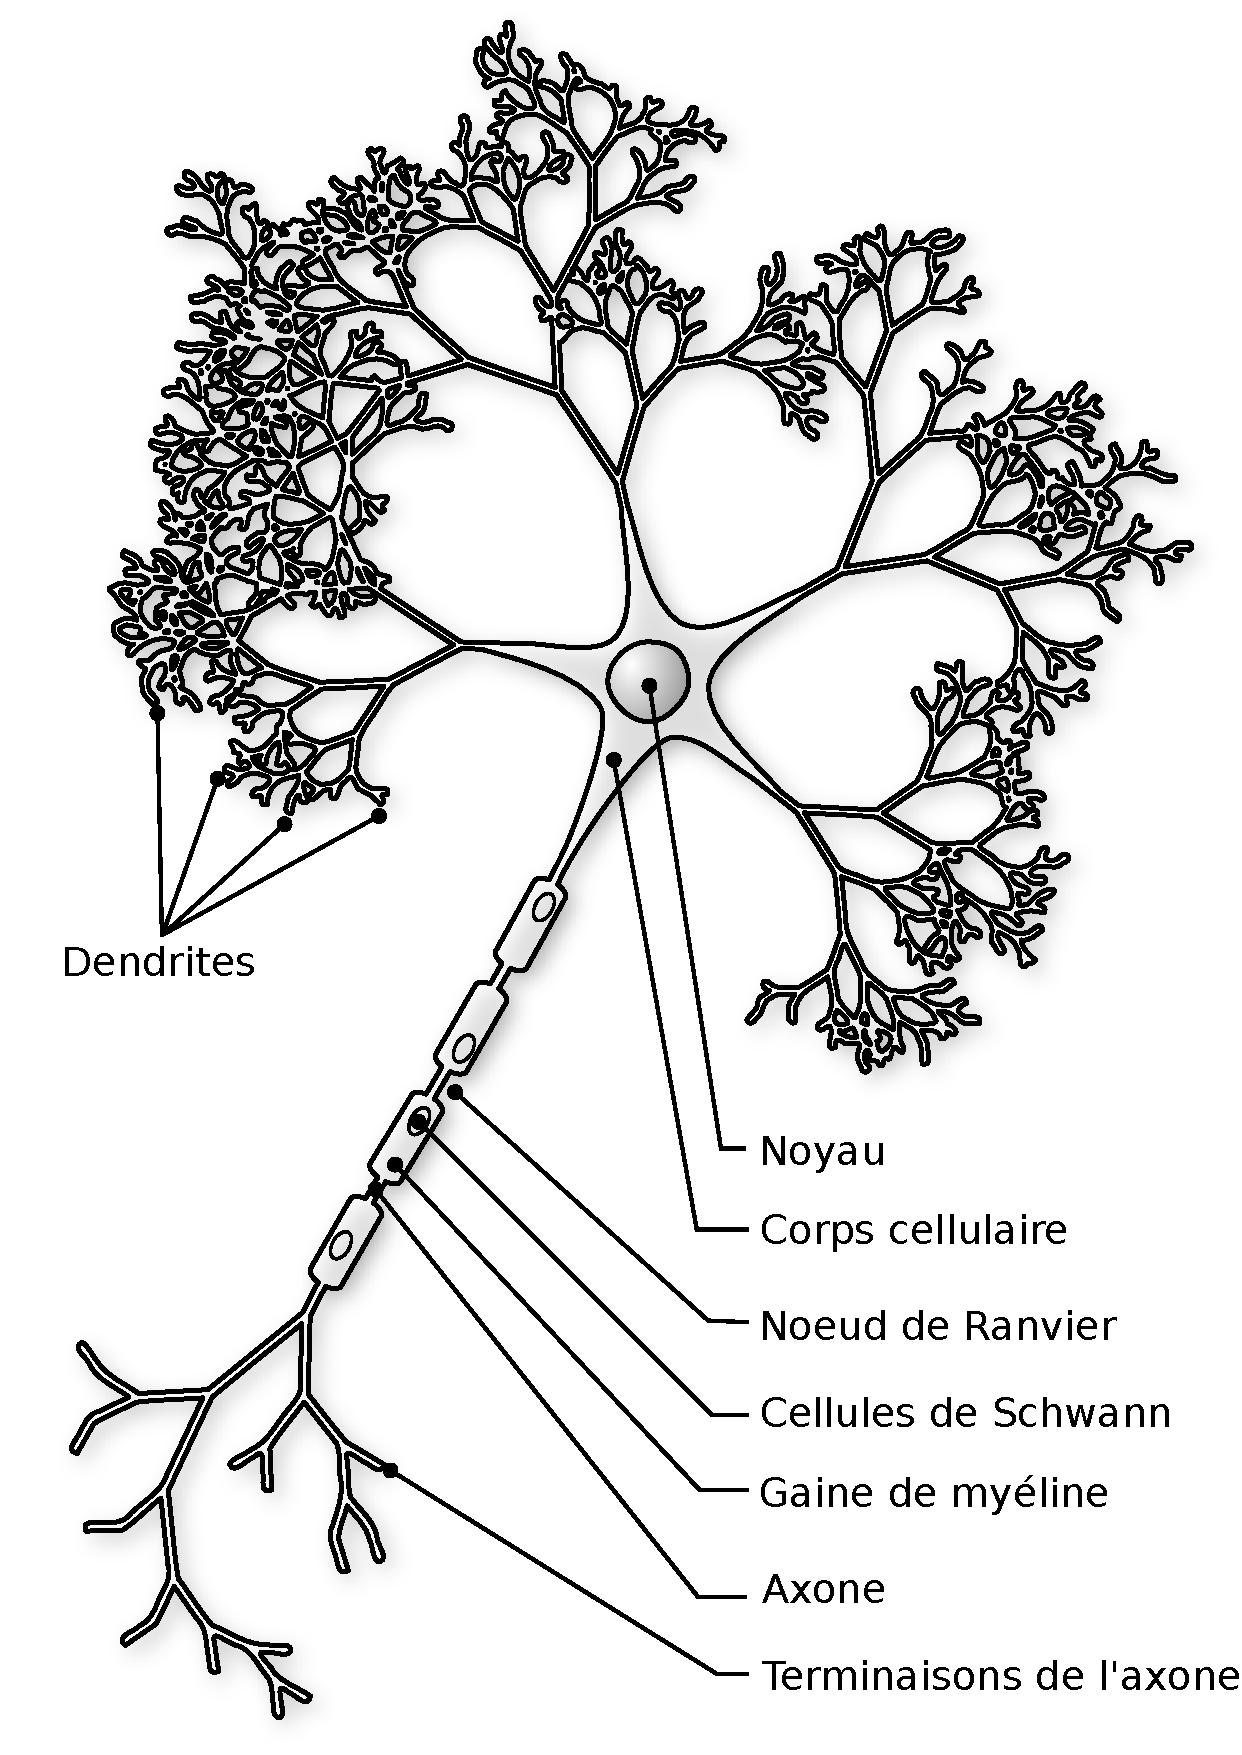
\includegraphics[height=0.5\textwidth]{figures/ch1_1_neurone}
\end{center}
\caption{Schéma d'un neurone biologique [wikipedia]}
\label{neurone}
\end{figure}

En effet, les membranes cellulaires en général, et les membranes des cellules nerveuses, en particulier, maintiennent une faible tension ou «potentiel» dans leur état normal de repos. Ce potentiel membranaire provient d'une différence de concentrations (entre l'extérieur et l'intérieur de la membrane) en électrolytes de calcium ($Ca^{2+}$), potassium ($K^{+}$) et sodium ($Na^{+}$). Un neurone est donc caractérisé par un potentiel de repos qui vaut généralement $-65mV$ mais qui peut varier selon le type de neurone considéré \cite{Kandel:2000}. Cette polarisation est assurée par l'action de canaux-ioniques voltage-dépendants qui régulent la concentration des ions. Quand le potentiel de membrane dépasse la valeur de repos, on parle de \textit{dépolarisation} et dans le cas contraire, on parle d'\textit{hyperpolarisation}. \\

Les variations du potentiel membranaire induisent de courtes impulsions électriques dont l'amplitude est d'environ $100mV$ et dont la durée moyenne est d'une milliseconde (fig \ref{potentiel}). Ces impulsions, appelées \textit{spikes} (pointes) ou \textit{potentiels d'action}, sont capables de se propager le long des axones permettant ainsi la transmission des informations. Nous aborderons dans la suite la question du codage neuronal. \\

\begin{figure}[htbp]
\begin{center}
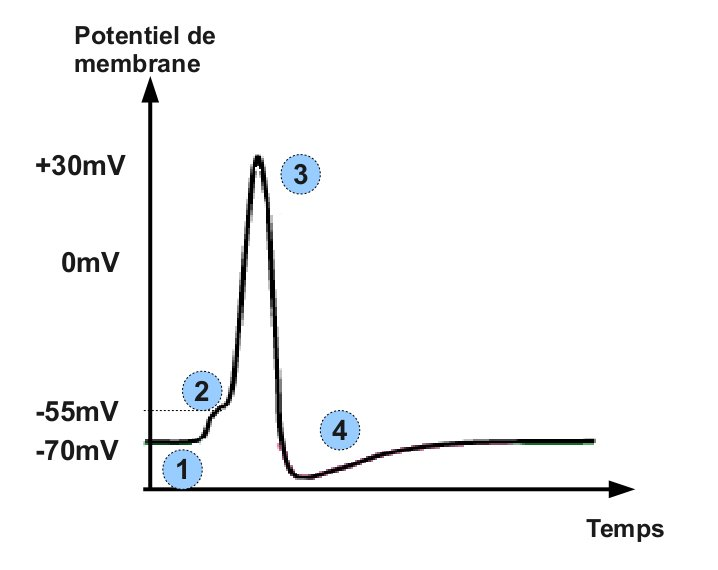
\includegraphics[width=0.4\textwidth]{figures/ch1_2_potentiel}
\end{center}
\caption{Les différentes phases du potentiel d'action. 1: prépotentiel, phase de repos. 2: dépolarisation de la membrane. 3: repolarisation rapide. 4: période réfractaire, hyperpolarisation.}
\label{potentiel}
\end{figure}

Les spikes sont des évènements discrets stéréotypés qui peuvent se produire à des intervalles réguliers ou pas. Ils se propagent le long de l'axone sans modifications. Une suite de potentiels est appelée \textit{train de spikes}. Ils sont généralement bien séparés, puisque un neurone passe par une \textit{période réfractaire} après l'émission d'un spike pendant laquelle il est silencieux (pas de spikes émis). \\

En effet, quand un spike arrive à une synapse à partir d'un neurone activé (neurone pré-synaptique), une substance chimique appelée neurotransmetteur est libérée provoquant l'ouverture des canaux ioniques dans la membrane du neurone au repos (neurone post-synaptique). Les ions circulent donc à travers les canaux créant un changement dans la polarisation membranaire de repos. Une variation temporaire dans la polarisation électrique de la membrane d'un neurone est appelée \textit{potentiel post-synaptique} [\gls{psp}]. Il s'agit d'un signal de réponse rapide très faible qui se déplace à travers la membrane et qui s'affaiblit en s'éloignant de son site de production. L'accumulation de \glspl{psp} reçus peut agir sur la probabilité d'émission de spikes, en particulier, quand la dépolarisation résultante est assez forte, le neurone se décharge: il émet un spike. Les \glspl{psp} sont appelés excitateurs (EPSP) s'ils augmentent la probabilité qu'un potentiel d'action post-synaptique se produise et inhibiteur (IPSP) s'ils diminuent cette probabilité.\\

La communication entre les neurones est assurée donc par ces transmissions de potentiels d'action. Leur génération fonctionne sur le mode ``tout ou rien'' puisqu'un spike ne peut être émis que si le seuil d'excitation du neurone est atteint. \\



En résumé, l'activité électrique des neurones est complexe. La communication entre eux est assurée par la transmission de potentiels d'action. Enfin, puisque les spikes sont d'amplitude et d'intensité invariables, un potentiel d'action isolé ne comporte qu'une petite partie de l'information. C'est plutôt le nombre et le timing de l'ensemble des spikes émis qui portent la majorité de l'information à traiter. Donc c'est la séquence de spikes émis qui contient le message transmis d'un neurone à un autre mais la question est de savoir quel est le code utilisé par les neurones pour traiter ce flux d'informations binaires?  \\  

%%%%%%%%%%%%%%%%%%%%%%%%%%%%%%%%%%%%%%%%%%%%%%%%%%%%%%%%%%%%%%%%%%%%%%%%%%%%%%%%%%%%%%%%%%%%%%%%%%%%%%%%%%%%%%%%%%%%%%%%%%%%%%%%%%%%%%%%%%%%%%%%%%%%%%%%%%%%%%%%%%%%%%%%%%%%%%%%%%%%%%%%%%%%%%%%%%%%
\subsection{Qu'est ce qui code l'information?}

Plusieurs expérimentalistes et théoriciens se sont intéressés à la question de savoir comment lire les trains de spikes (\ref{train}) pour comprendre la communication neuronale. Plusieurs propositions existent \cite{Shadlen:1994, Rieke:1996, Borst:1999,  Gerstner:2002, Pouget:2003, Averbeck:2004, Cariani:2004}.\\


\begin{figure}[htbp]
\begin{center}
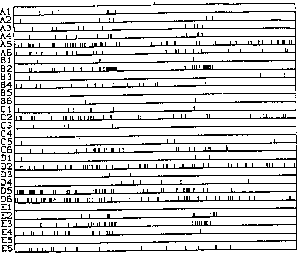
\includegraphics[width=0.4\textwidth]{figures/ch1_3_train}
\end{center}
\caption{Exemple d'enregistrement de trains de spikes de 30 neurones. Chaque ligne correspond à un neurone. L'axe horizontal représente le temps (en total 4000ms). Chaque impulsion est représentée par un petit trait vertical (Kruger et Aiple, 1988)}
\label{train}
\end{figure}

La question que l'on se pose porte sur l'information contenue dans une telle représentation spatio-temporelle des spikes: quel est le code utilisé pour transmettre ces signaux et quel est le mécanisme utilisé par les autres neurones pour les décoder ?\\

Deux stratégies de codage sont généralement décrites. La première stratégie est le codage \textit{fréquentiel} qui consiste à compter les spikes et les moyenner par rapport au temps, par rapport aux essais expérimentaux ou par rapport aux populations de neurones pour déterminer un niveau d'activité. Plusieurs études supposent que la plupart de l'information est contenue dans \textit{la fréquence moyenne de décharge} qui est devenue un outil standard pour décrire les propriétés des neurones sensoriels ou corticaux \cite{Mountcastle:1957, Hubel:1959}. Cependant, une telle hypothèse néglige l'information contenue dans les dates d'occurences individuelles des spikes \cite{Oram:1999, Abeles:1994, Hopfield:1995, Bialek:1991, Shadlen:1994, Rieke:1996}. La seconde stratégie de codage, dite \textit{impulsionnelle}, repose sur le profil temporel de la séquence de spikes. Elle permet de conserver l'information temporelle concernant les impulsions individuelles, sur une échelle de temps d'une milliseconde \cite{Rieke:1997}. Nous passerons d'abord en revue certaines méthodes de codage impulsionnel. Ensuite nous nous concentrerons sur le codage fréquentiel. 


\subsubsection{Codage impulsionnel}
Nous allons présenter ici trois stratégies possibles du codage impulsionnel (codage à spikes): 
\paragraph{Les premiers spikes décident:}

\cite{Thorpe:1996} propose que la rapidité de la réponse dans des tâches de discrimination visuelle implique que la décision se fait dès les tous premiers spikes. Il fait valoir que le cerveau n'a pas le temps d'évaluer plus d'un spike de chaque neurone par étape de traitement. Il suppose donc que le premier spike contient la majorité de l'information pertinente. Cette stratégie reste un modèle très simplifié de codage.


\paragraph{Phases:}

Le codage par phase a été étudié expérimentalement \cite{Okeefe:1993} et théoriquement dans plusieurs modèles \cite{Hopfield:1995, Maass:1996, Jensen:1996}. Il s'agit d'un codage basé sur le retard relatif d'un neurone par rapport à d'autres. Cette méthode a permis d'expliquer, par exemple, le codage de la localisation spatiale dans l'hippocampe du rat  \cite{Okeefe:1993} (le temps de décharge code l'emplacement du rat dans le lieu auquel la cellule correspondante est sensible). 


\paragraph{Synchronie et corr\'elations:}

Ce codage postule que l'information peut aussi être contenue dans la synchronisation entre des neurones ou entre un neurone et un autre signal physiologique. Par exemple, l'analyse de l'activité des neurones visuels dans le corps genouillé latéral a montré que beaucoup plus d'information sur le stimulus peut être extraite à partir de leurs trains de spikes si les pics qui coïncident sont pris en compte séparément \cite{Alonso:1996}. Le rôle exact des corrélations et des synchronisations dans la réponse à un stimulus n'est pas encore clair. Une hypothèse est de considérer que la synchronisation entre les paires de neurones dans le cortex visuel signale si ces neurones répondent à un même objet ou à deux objets distincts \cite{VonderMalsburg:1992, Eckhorn:1988, Gray:1989}.\\

En résumé, plusieurs études se sont intéressées au codage de l'information dans l'organisation temporelle des spikes. En particulier, les travaux de \cite{Thorpe:1996} insistent sur l'importance de la latence du premier potentiel d'action. Les modèles à spikes représentent de manière simplifiée l'activité électrique des neurones en se basant sur la temporalité des potentiels d'actions et non pas sur la variation de leur activité électrique. 

\subsubsection{Codage fréquentiel}

Le codage fréquentiel se base sur l'hypothèse que la majorité de l'information codée par un neurone réside dans la fréquence moyenne d'émission de potentiels d'actions, appelée aussi \textit{fréquence moyenne de décharge} [\gls{msr}]. En effet, le codage fréquentiel propose de compter les spikes pour déterminer le niveau d'activation. Comme décrit dans \cite{Gerstner:2002}, il existe trois façons d'estimer cette moyenne, à savoir, temporelle, stochastique et par population.\\

\paragraph{Moyenne temporelle}

La \gls{msr} est interprétée comme le nombre de spikes qui sont émis dans un intervalle de temps donné $T$ divisé par $T$. Cet intervalle est défini par l'expérimentateur et le type de neurone utilisé pour les enregistrements \cite{Adrian:1926, Kandel:1991}. Supposons que nous représentons une séquence de spikes à des moments ${t_0,t_1,. . . , t_n}$. On peut donc approximer la valeur empirique de la \gls{msr} par une variable continue $\nu$:\\

\begin{center}
\begin{equation} 
\nu(t) = \frac {\sum_{i=0}^{n}{\delta (t-t_i)}}{T} =\frac{N_ {spikes} (T) }{T}
 \end{equation}
\end{center}

Il est nécessaire d'attendre une durée assez longue avant d'avoir une estimation fiable d'autant plus que les vrais trains de spikes sont très irréguliers, une estimation fiable de la \gls{msr} par moyenne temporelle nécessite un grand nombre de décharges. Ceci n'est pas en accord avec certaines constatations biologiques. Par exemple, une mouche peut réagir à des stimuli visuels et changer sa direction du vol dans les 30 à 40 ms \cite{Rieke:1997}. En outre, l'homme peut reconnaître certains aspects de scènes visuelles rapidement \cite{Thorpe:1996, Keysers:2001}.\\

\paragraph{Moyenne Stochastique}

Une autre définition de la \gls{msr} correspond à la moyenne sur plusieurs essais expérimentaux. La même séquence de stimuli est présentée k fois. Pour chaque essai le temps est divisé en fenêtres $\Delta t$ de largeur de l'ordre de quelques millisecondes. Le nombre de spikes émis entre $t$ et $t+\Delta t$ est compté pour chaque essai permettant d'estimer l'activation typique du neurone. D'où l'équation suivante:\\

\begin{center}
\begin{equation} 
\nu(t)= \frac {1}{\Delta t}\frac{N_ {k} (t,t+\Delta t) }{k} 
 \end{equation}
\end{center}

Un problème évident de cette approche est qu'elle ne peut pas être utilisée par les neurones dans le cerveau. L'exemple donné par \cite{Gerstner:2002} est qu'une grenouille ne peut pas attraper une mouche en attendant que l'insecte vole à plusieurs reprises le long de la même trajectoire, elle doit agir sur un seul essai!\\

\paragraph{Moyenne spatiale : codage par population }

Shadlen et Newsome \cite{Shadlen:1994}, proposent qu'une estimation fiable de la \gls{msr} peut être obtenue en calculant la moyenne instantanée de spikes émis par environ 100 neurones équivalents sans recourir à des calculs classiques de la moyenne temporelle. Il s'agit d'un codage par population \cite{Wu:2002}, donc plutôt spatial.\\

La \gls{msr} est interprétée comme l'\textit{activité} moyenne d'une population de neurones équivalents. Le mot \textit{équivalent} signifie que tous les neurones ont une connectivité identique et reçoivent le même type d'entrée. Souvent de nombreux neurones ont des propriétés similaires et répondent aux mêmes stimuli. Par exemple, les neurones du cortex visuel primaire des chats et des singes sont disposés en colonnes de cellules ayant des propriétés similaires \cite{Hubel:1988, Hubel:1962, Hubel:1977}. Le bruit, cependant, est différent pour chaque neurone permettant d'avoir des réponses différentes à une même entrée. L'activité de la population est définie comme la fraction des neurones qui sont actifs dans un court intervalle [t, t + $ \Delta t$] divisé par $\Delta t$. La fréquence moyenne de décharge correspond donc à diviser cette activité totale par le nombre $N$ de neurone dans la population. 

\begin{center}
\begin{equation} 
\nu(t) =\frac{1}{N} \frac{N_ {spikes,population} (t,\Delta t) }{\Delta t} 
 \end{equation}
\end{center}

Quand $N$ tend vers l'infini, l'activité A peut être approchée par une variable analogique qui varie de manière continue dans le temps et elle garde la dimension d'une fréquence, égale au nombre de spikes émis instantanément.\\

Une des propriétés utiles de l'activité moyenne de la population est qu'elle peut réagir très rapidement aux changements dans les entrées \cite{Brunel:2001,Gerstner:2000}. En outre, même si une population réelle présente toujours un certain degré d'hétérogénéité, le principe reste intéressant et la définition peut être modulée en utilisant une moyenne pondérée sur la population. \\

Enfin, théoriquement, un neurone qui reçoit une entrée constante, émet un train de spikes régulier (intervalle de temps constant entre les impulsions). $\nu$ est donc simplement l'inverse de l'intervalle temporel inter-spikes. Si l'entrée du neurone augmente, sa \gls{msr} augmente jusqu'à ce qu'elle sature à un taux maximal $\nu_{max}$. Un neurone ne peut pas émettre des spikes au-delà d'une certaine fréquence.\\

Plus généralement, on peut dire que le potentiel de membrane est transformé en activation (\gls{msr}) d'o\`u $\nu = f(V)$ avec $V$ le potentiel post-synaptique (PSP, \textit{post synaptic potential}) et $f$ la \textit{fonction de gain} du neurone ou encore appelée fonction \textit{d'activation}, fonction \textit{de transfert}, fonction de \textit{décharge}.

\subsubsection{Fonction d'activation }

La fonction d'activation représente une approximation de la relation entre l'état interne du neurone (potentiel de membrane) et la \gls{msr} qui permettrait dans le cadre d'un codage fréquentiel de se passer d'expliciter les trains de spikes. La figure (fig.\ref{gain}) montre quelques exemples de fonctions d'activation. La plus simple est celle de Heaviside et une fonction couramment utilisée est la fonction sigmoïde \cite{Wilson:1972, Amari:1977}.\\


\begin{figure}[htbp]
\begin{center}
\begin{tabular}{|c|c|c|}
\hline
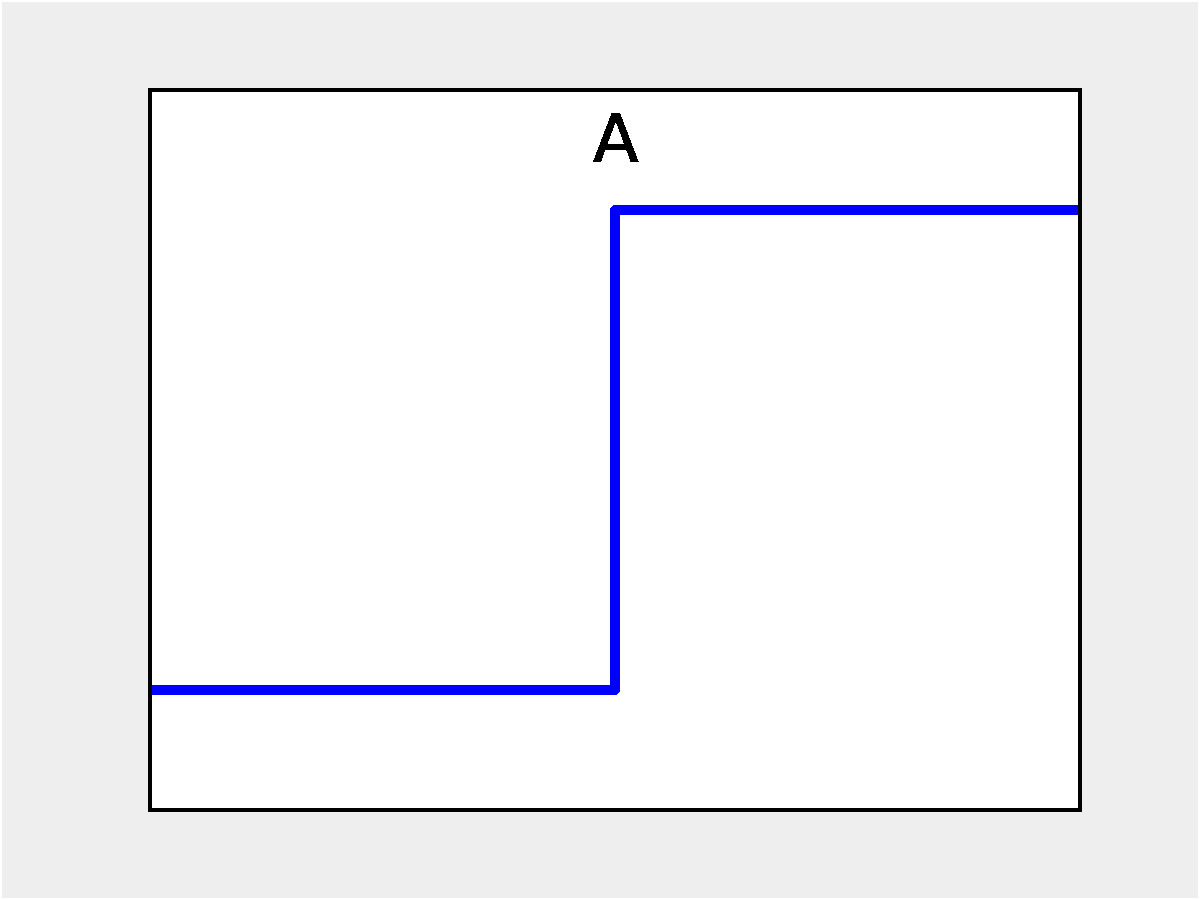
\includegraphics[width=0.3\textwidth]{figures/ch1_4_profile-heaviside}
&
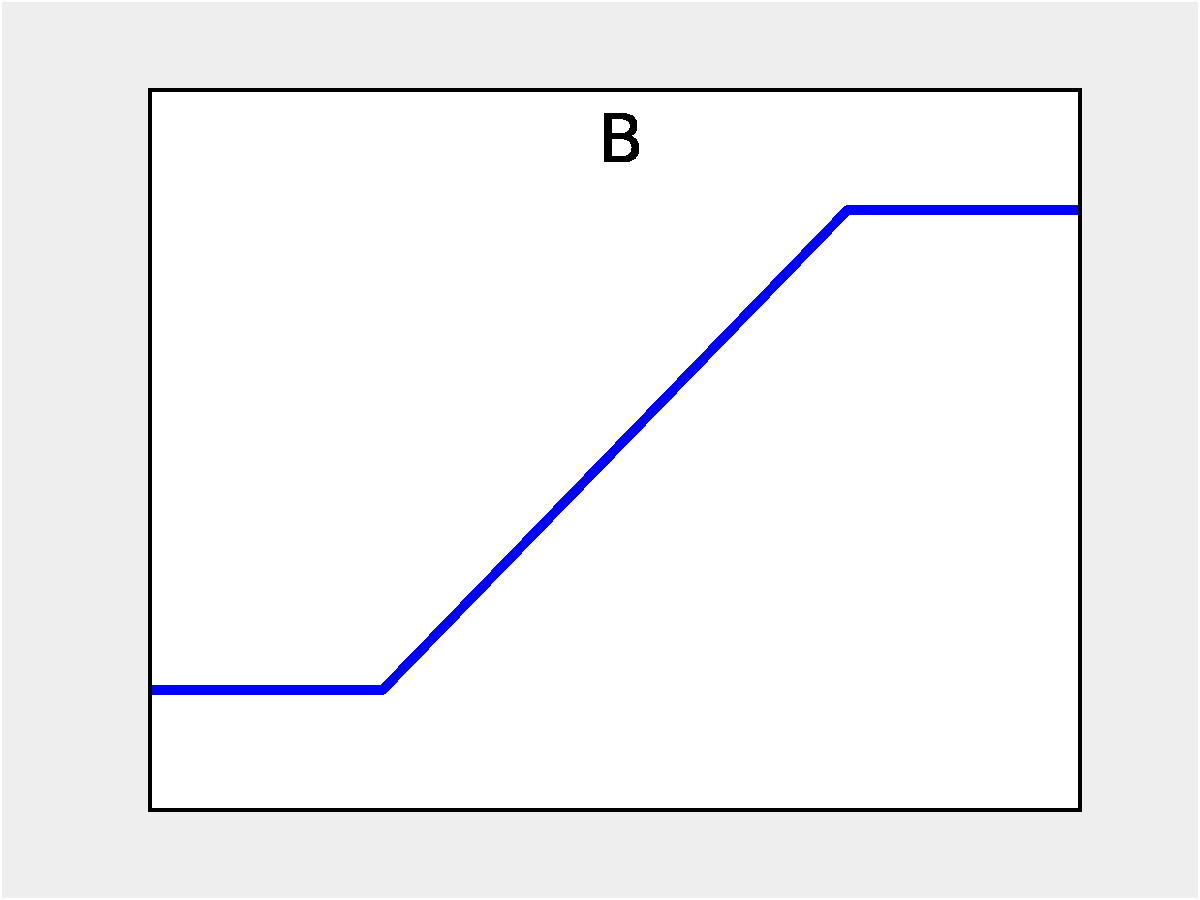
\includegraphics[width=0.3\textwidth]{figures/ch1_4_profile-linear}
&
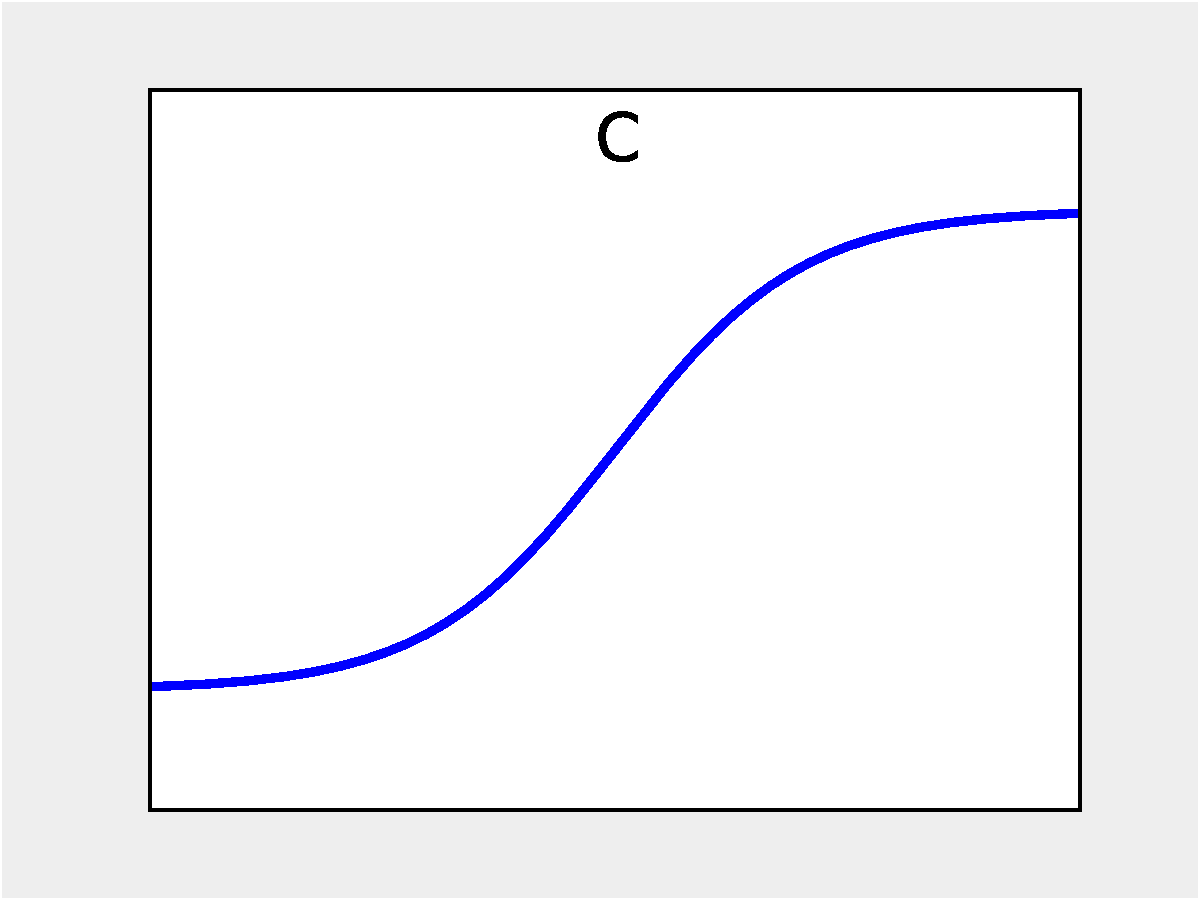
\includegraphics[width=0.3\textwidth]{figures/ch1_4_profile-sigmoid}\\
\hline
\end{tabular}
\end{center}
\caption{Exemples de fonctions de gain fréquemment utilisées pour les modèles fréquentiels. La fréquence moyenne de tir $\nu$ est représentée en fonction de la valeur de l'entrée $I$ qui peut être interprétée comme un potentiel d'action provenant d'un autre neurone. A: une fonction de Heaviside. B: une fonction linéaire par morceaux. C: une fonction sigmoïde }
\label{gain}
\end{figure}

Prenons maintenant le schéma d'interaction entre un neurone post-synaptique $i$ et plusieurs neurones pré-synaptiques $j$ tel qu'il est décrit par Ermentrout \cite{Ermentrout:1980}. $V_i(t)$ est le potentiel de membrane du neurone $i$ à l'instant t qui sera transformé en activation $\nu_i(t)=f(V_i(t))$ qui sera transmise vers d'autres neurones via l'axone.\\

Un neurone est caractérisé donc d'une part par sa fonction de gain. D'autre part, l'évolution de son état dans le temps peut être décrite par l'une des équations suivantes qui reposent sur deux approximations différentes d'une même équation globale plus complexe : 

\begin{center}
\begin{equation} 
\tau_i \frac{dV_i}{dt}+V_i= \sum_{j} {w_{ij} f_j(V_j)} 
 \end{equation}
\label{vol}
\end{center}

\begin{center}
\begin{equation} 
\tau_i \frac{dU_i}{dt}+U_i= f(\sum_{j} {w_{ij} U_j} )
 \end{equation}
\label{act}
\end{center}

La première équation est une version simplifiée du modèle intégrateur-à-fuite détaillé dans la suite. On retient que dans cette version la variable principale est le potentiel de membrane et que la fonction d'activation est à l'intérieur de la somme. La deuxième équation correspond aux modèles basés plutôt sur l'activation synaptique moyenne <U> \cite{Gutkin:2003, Wilson:1972, Pinto:1996}. Pour plus de détails voir \cite{Ermentrout:1998}.\\

Enfin, l'étude de la régularité de l'activité corticale constitue un point central dans le débat sur le codage impulsionnel ou fréquentiel. La décharge corticale a souvent été considérée comme irrégulière, proche d'un processus de Poisson, donc en faveur d'un codage impulsionnel. Mais des études récentes ont montré que la décharge d'un neurone du cortex auditif en réponse à un ton pur est plutôt binaire que Poisson \cite{DeWeese:2003}. En outre, une activité régulière de certains neurones dans les aires pariétales, en particulier le cortex moteur, a été rapportée \cite{Lee:1998, Maimon:2009}, donc en faveur d'un codage fréquentiel.\\

En résumé, l'information neuronale peut être codée de diverses manières \cite{Perkel:1968}. Les stratégies de codage fréquentiel et impulsionnel sont toujours sujettes à controverses. Les deux paradigmes semblent co-exister et selon la fonction (et la structure) étudiée, la pertinence de l'un ou l'autre l'emporte. Il en résulte donc plusieurs modèles de neurones artificiels. Nous présenterons dans la suite quelques familles de ces modèles.

\subsection{Le neurone artificiel}

\textit{Le neurone formel} est historiquement le premier modèle inspiré du neurone biologique. Le neurone formel est une fonction mathématique bornée qui prend plusieurs entrées (valeurs des variables) et donne une sortie (valeur de la fonction) qui correspondent respectivement aux dendrites du neurone biologique et son axone.\\

Le premier modèle de neurone formel a été proposé par un neurologue français appelé Louis Lapique en 1907. Des modèles plus réalistes, qui décrivent finement le fonctionnement électrique des neurones, ont été ensuite développés. Il s'agit des modèles de neurones \textit{implusionnels}. Ces modèles permettent de reproduire des mesures électrophysiologiques avec beaucoup de précision permettant donc de mettre en oeuvre un codage à spikes. D'autres modèles, comme le neurone \textit{intégrateur-à-fuite}, se basent plutôt sur le codage fréquentiel. 

\subsubsection{Neurone impulsionnel}

Les modèles impulsionnels se focalisent sur les phénomènes électriques en considérant les neurones comme des systèmes dynamiques dont la variable d'état principale est souvent \textit{le potentiel de membrane}.\\

\begin{figure}[htbp]
\begin{center}
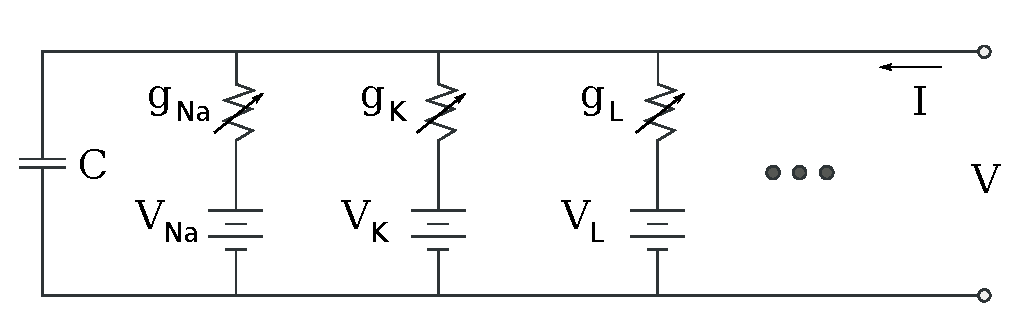
\includegraphics[width=0.5\textwidth]{figures/ch1_5_Hodgkin-huxley-circuit.pdf}
\end{center}
\caption{Schéma électrique du modèle Hodgkin-Huxley. Le courant ionique à travers la membrane peut être divisé en trois composants: courant de sodium ($I_K$), courant de potassium ($I_{Na}$) et une petite fuite de courant ($I_L$) causée par d'autres ions. Chaque composant peut être exprimé en termes de potentiel de repos de la cellule ($V$), des potentiels d'équilibre respectifs pour chaque composant ($V_K$, $V_{Na}$ et $V_L$), des constantes reflétant la conductance de chaque composant ($g_K$, $g_{Na}$ et $g_{L}$) et des variables supplémentaires ($n$, $m$ et $h$).}
\label{Hodgkin}
\end{figure}

Le modèle impulsionnel central est celui de A. Hodgkin et A. Huxley \cite{Hodgkin:1952} qui leur a valu le prix Nobel en 1963. Il décrit quantitativement comment les \textit{potentiels d'action}~(fig \ref{potentiel}) sont générés et propagés dans l'axone à travers un modèle mathématique basé sur un système d'équations différentielles couplées. Ce modèle fait intervenir des variables représentant les conductances des canaux ioniques. La membrane peut donc être représentée comme un circuit éléctrique~(voir fig.\ref{Hodgkin}).\\



\subsubsection {Neurone intégrateur-à-fuite}

Le modèle de neurone \textit{intégrateur-à-fuite} est l'un des modèles les plus populaires qui permet d'utiliser un codage fréquentiel (voir \cite{Blynel:2002} pour un aperçu sur le comportement des neurones intégrateur-à-fuite). Nous détaillerons ce modèle qui nous servira de modèle de neurone dans le chapitre 4. Il est basé sur l'hypothèse que les unités de base de calcul dans les systèmes nerveux sont les neurones individuels. L'état d'un neurone $i$ est décrit à l'instant $t$ par le potentiel de membrane $u_i$, régi par l'équation différentielle suivante :

\begin{center}
\begin{equation} 
\tau\frac{du_i(t)}{dt}= -u_i(t)+\sum_j {f(u_j(t))w_{ij}} + \sum_k {s_{ik}} +\theta
 \end{equation}
\end{center}

o\`u $\tau$ est la constante de temps. Le neurone compte une somme linéaire des entrées qu'il reçoit. La première somme s'étend sur tous les neurones $j$ qui renvoient des signaux au neurone $i$, la seconde somme s'étend sur l'ensemble des entrées externes $s_{ik}$. $w_{ij}$ décrit la force de la connexion synaptique entre les neurones $i$ et $j$. $f$ est la fonction d'activation. En l'absence d'entrées, le potentiel de membrane se relaxe vers le niveau de repos $\theta$.\\

Le terme \textit{intégrateur} décrit la capacité des neurones à intégrer l'activation entrant au fil du temps. Le terme \textit{fuite} signifie qu'une certaine quantité d'activation du neurone est perdue sur le neurone à chaque pas de temps, de sorte que son niveau d'activité décroît progressivement vers le niveau de repos en l'absence d'apport des entrées. La vitesse d'intégration des activations d'entrée et de décroissance de l'activation interne est commandée par la constante de temps $\tau$. Ainsi l'activation des neurones change de manière continue (lisse) sur plusieurs pas de temps au lieu de varier brusquement permettant ainsi de contrôler des actions plus naturelles.\\

En plus de ces modèles qui permettent de garder certaines propriétés du neurone biologique, une autre approche qui s'inspire du fonctionnement du cerveau sans chercher à le reproduire finement a été explorée. Dans ce type d'approche, la dynamique est complètement laissé de côté, seul le résultat du traitement de l'information importe. \cite{McCulloch:1943} ont proposé un modèle de neurone formel qui réalise une fonction d'intégration simple d'informations reçues des autres neurones formels. Les entrées sont pondérées par des coefficients (\textit{poids}) approchant les caractéristiques des synapses (fig\ref{Albin}). Le modèle réalise une somme pondérée des entrées suivie d'une non-linéarité (fonction de Heaviside). L'état de sortie du modèle est soit $0$, soit $1$ (activé ou non-activé). Les auteurs distinguent les entrées excitatrices des entrées inhibitrices. Une variante du modèle consiste à utiliser des poids négatifs pour les entrées inhibitrices et des poids positifs pour les entrées excitatrices. Ensuite si la somme dépasse une valeur seuil prédéfinie, la sortie sera $1$, sinon $0$.\\

\begin{figure}[htbp]
\begin{center}
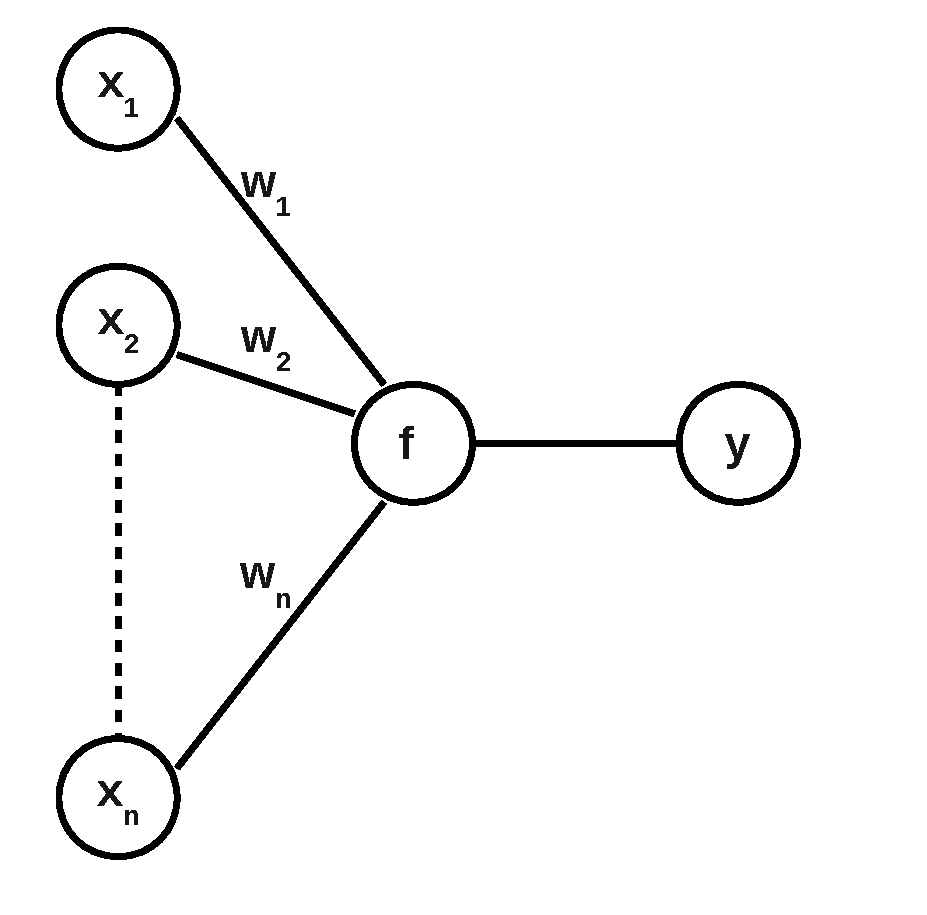
\includegraphics[height=0.3\textwidth]{figures/ch1_6_formel}
\end{center}
\caption{Le neurone formel réalise une fonction non linéaire bornée qui prend plusieurs entrées $x_i$ (entrées pré-synaptiques) pondérées par des poids de connexion $w_i$ et retourne une sortie (sortie post-synaptique) $ y = f (x_1, x_2, ..., x_n; w_1, w_2, ..., w_n)$. }
\label{formel}
\end{figure}

Enfin, le neurone comme unité isolée reste une fonction simple qui n'a pas d'énormes capacités de calcul. C'est l'association de tels éléments simples sous la forme de réseaux qui permet de réaliser des fonctions utiles permettant de résoudre des problèmes complexes. On passe donc à un codage permettant de faire des calculs distribués, o\`u chaque unité détient une partie de l'information.\\

En particulier, McCulloch et Pitts ont montré comment des systèmes neuronaux pourraient mettre en œuvre une logique du premier ordre. Influencés par les travaux de Nicolas Rashevsky dans les années 1930 qui suggère que le cerveau pourrait être vu comme une organisation de 0 et de 1 (la première édition de son livre \textit{Mathematecal biophysics} en 1938), ils ont introduit des réseaux de neurones discrets dans le temps et avec des variables booléennes comme un modèle du fonctionnement du cerveau. Cela nous amène à la théorie connexionniste résultant des deux constatations suivantes: D'une part, la mise en commun d'unités simples permet d'acquérir de vastes capacités de traitement de l'information \cite{Rashevsky:1960}, d'autre part, \cite{Hebb:1949} a introduit une règle d'apprentissage décrivant comment les interactions entre plusieurs neurones permet de modifier le comportement de l'ensemble.


\section{Approche connexionniste: Les réseaux de neurones}

La théorie du \textit{connexionnisme} issue des travaux de \cite{Hebb:1949, Hayek:1952} est une approche qui modélise les fonctions cognitives complexes comme des processus émergents d'un ensemble d'unités simples interconnectées utilisant des calculs locaux simples. Cet ensemble d'unités forme ce qu'on appelle un \textit{réseau de neurones}. La forme des connexions et les caractéristiques des unités peuvent varier selon les modèles. Par abus de langage on confond souvent les termes neurone (biologie), unité (unité de calcul), cellule (automate cellulaire) et neurone artificiel (connexionisme).\\

Le \textit{perceptron} est l'un des premiers réseaux de neurones artificiels, il résulte des travaux de Rosenblatt \cite{Rosenblatt:1958}. C'est un modèle inspiré du système visuel. Il est constitué de seulement deux couches de neurones, une couche d'entrée (dite \textit{perceptive}) qui correspond aux neurones sensoriels qui reçoivent les stimuli du monde externe et une couche de sortie (dite \textit{décisionnelle}) qui correspond aux neurones moteurs qui restituent les résultats au monde externe. Les neurones de la couche d'entrée projettent sur les neurones de la couche de sortie selon des jonctions (des connexions). On associe un poids synaptique à chaque jonction, de sorte que les entrées sont multipliés par ce poids, puis additionnées par les neurones de sortie, ce qui est équivalent à multiplier le vecteur d'entrée par une matrice de transformation.\\

Dans ce type de réseaux les connexions se font dans un seul sens (\textit{feedforward}) par opposition aux réseaux dit \textit{récurrents} \cite{McCulloch:1943} dans lesquels les sorties de certaines unités sont retournées vers des unités de la couche d'entrée. En plus, il est supposé implicitement qu'il n'y a pas d'organisation spatiale des connexions. Cependant, il existe dans le cortex et dans d'autres régions cérébrales des répartitions spatiales claires des connexions entre les différentes unités neuronales. Nous examinerons dans la suite des modèles de réseaux de neurones dynamiques qui prennent en compte ces constatations.\\

En effet, le nombre de neurones et de synapses dans une petite partie du cortex étant immense, l'hypothèse de considérer une couche de neurones comme un continuum dans l'espace a été adoptée par plusieurs chercheurs dans le cadre de la théorie des champs neuronaux continus (CNFT, \textit{continuum neural field theory}) \cite{Wilson:1973, Amari:1977}. Cette théorie s'inspire de la théorie \textit{des champs continus} en physique défendue par Albert Einstein. L'évolution de l'état interne du champ neuronal est décrite par une équation différentielle dépendant de l'espace et du temps. Le profil des connexions dépend lui aussi du positionnement dans l'espace.\\

Considérons la version généralisée d'un champ neuronal dynamique (DNF, \textit{dynamic neural field}) avec des délais de transmission, qui décrit l'évolution spatio-temporelle du potentiel de membrane dans une population de neurones. Nous allons considérer un seul réseau (\textit{champ}) $M$ composé de plusieurs unités avec des connexions spatiales entre elles. Chaque unité, au niveau mésoscopique biologique, peut correspondre à une colonne corticale \cite{Chemla:2007}. Le réseau représente donc une carte corticale (voir par exemple \cite{Vieville:2007} pour une discussion sur le concept), et peut être modélisé par un DNF continu dans l'espace \cite{Wilson:1973, Taylor:1999, Amari:1977}. L'évolution du potentiel de membrane $ V $ d'une unité dans un tel réseau est décrite par l'équation différentielle suivante:\\
%%
\begin{align}
  \label{eq: DNF-continuous}
  & \frac{\partial V(\mathbf{x},t)}{\partial t} =
  -\frac{1}{\tau(\mathbf{x})} \, V(\mathbf{x},t) + h(\mathbf{x}, t) + s(\mathbf{x}, t) 
  &+ \int_{\cal M} d \mathbf{y} \, \int_0^{+\infty} \, \hspace{-1em} d \eta \; W(\mathbf{x}, \mathbf{y}, \eta) \, \sigma_{\mathbf{y}}\left(V(\mathbf{y}, t - \eta)\right) 
\end{align}
%%

où $\mathbf {x}$ désigne une position dans le champ continu $M$, $t$ est le temps, $V(\mathbf{x},t)$ désigne le potentiel de membrane au point $\mathbf {x}$ à l'instant $t$, $ {\tau} $ est la constante temporelle caractéristique des synapses, $\eta$ est le délai de transmission, $ W $ est la fonction de connexions synaptiques, $ s(\mathbf {x},t) $ est l'entrée reçue à la position $ \mathbf {x} $ et $ h $ est le seuil moyen du neurone. Dans ce cadre, $ \sigma_ {\mathbf{y}} ()$ est une fonction sigmoïde qui représente la fonction d'activation du neurone à la position $y$. \\

Certains modèles de DNF supposent que la vitesse de transmission des signaux dans le réseau n'est pas bornée, donc négligent les délais de transmission (i.e., $W({\bf x}, {\bf y}, \eta) = w({\bf x}, {\bf y}) \, \delta(\eta - 0)$, avec seulement des transmissions \textit{instantanées}). D'autres considèrent une transmission constante, avec un retard (e.g., $W({\bf x}, {\bf y}, \eta) = W({\bf x}, {\bf y}) \, \delta(\eta - \frac{|{\bf x} - {\bf y}|}{v})$ pour une vitesse de propagation $v$). La formulation précédente englobe ces différents cas, en tenant compte de la nature spatio-temporelle de la connexion. \\

Enfin, l'un des principaux intérêts des réseaux connexionnistes est leur capacité d'\textit{apprentissage}. Biologiquement, il s'agit de modifier la transmission synaptique, ce qui nous ramène à la notion de \textit{plasticité synaptique}.  Il s'agit d'une sous-partie d'une propriété plus large du réseau neuronal et du cerveau en général: la plasticité neuronale (ou cérébrale). Le cerveau est qualifié donc de ``plastique'' (en perpétuelle reconfiguration), il se modifie et s'adapte par l'expérience. Nous examinerons cette notion dans la section suivante.\\


\section {Calcul adaptatif : Plasticité et apprentissage}
 

La plasticité synaptique repose sur le fait que l'efficacité d'une synapse peut varier au cours du temps. Elle englobe tous les mécanismes intervenant dans la modification de la transmission synaptique au cours du temps. En effet, la connexion entre deux neurones n'est pas figée mais dépend de l'activité précédente des neurones et de l'utilité de cette connexion dans la génération du résultat final. \\

La première règle proposée pour la plasticité, dans le cadre de l'apprentissage, est celle de Hebb \cite{Hebb:1949, Gerstner:2002} qui postule qu'une synapse devient plus efficace quand elle participe à l'activation du neurone post-synaptique. Ce postulat implique que l'augmentation de l'efficacité synaptique nécessite une corrélation temporelle entre l'activation des deux neurones (décharger de manière rapprochée) qui peut traduire un lien de causalité. La règle d'apprentissage de Hebb se formule de la manière suivante \textit{``quand une cellule A excite de manière répétée une cellule B, l'efficacité de A à exciter B est améliorée par des changements métaboliques''}. Considérons une synapse avec une efficacité $w_{ij}$ permettant de transmettre des signaux d'un neurone pré-synaptique $i$ vers un neurone post-synaptique $j$. On se contente ici de la formulation en termes de fréquence moyenne de décharge. Dans la suite, l'activité du neurone pré-synaptique est notée $\nu_i$ et celle du neurone post-synaptique est notée $\nu_j$. La variation de l'efficacité synaptique, selon la règle de Hebb, est donnée par l'équation générale suivante:\\

\begin{align}
\frac{\delta w_{ij}}{\delta t}=G(w_{ij};\nu_i,\nu_j)
\end{align}

Cette formulation souligne le caractère local de la règle, mais un autre aspect important du postulat de Hebb est l'effet cooperatif. Ils faut que les neurones pré- et post-synaptiques s'activent simultanément pour que le poids synaptique change. D'o\`u l'exemple particulier de la fonction $G$ dans l'équation suivante:

\begin{align}
\frac{\delta w_{ij}}{\delta t}=\alpha \nu_i \nu_j
\end{align}

 où la variable $\alpha$ est appelée le coefficient d'apprentissage.\\

Dans la version initiale, seul le renforcement est envisagé ($\alpha >0$) et en absence de mécanisme complémentaire, les synapses seraient saturées à leur poids maximal. C'est ainsi qu'un postulat complémentaire a été proposé par \cite{Stent:1973}:\textit{"Quand un neurone pré-synaptique A échoue de manière répétée et persistante à exciter un neurone B post-synaptique tandis que cette cellule décharge sous l'influence d'autres neurones pré-synaptiques, un changement métabolique se produit dans la voie entre les deux cellules de manière à ce que l'efficacité de A est diminuée"}. On parle donc de \textit{dépression synaptique}.\\

Plus généralement, il s'agit d'une règle d'apprentissage \textit{non-supervisé} (apprendre sans professeur) qui sera décrite brièvement dans la suite ainsi que les deux autres types d'apprentissage : \textit{supervisé} (apprendre à trouver la bonne réponse à une demande spécifique) et \textit{par renforcement} (apprendre par interaction avec l'environnement via la récompense).\\

\subsection{Apprentissage supervisé}

L'apprentissage supervisé consiste à apprendre une tâche en se basant sur l'erreur entre la réponse fournie par le modèle et la réponse attendue connue par l'expérimentateur (le professeur). Ce dernier doit fournir au système un échantillon d'entrées possibles ainsi que les réponses désirées correspondant à ces entrées. Pour chaque entrée, le réseau fournit une réponse qui sera comparée à la réponse désirée, ensuite les poids sont ajustés de manière à ce que la sortie soit le plus proche possible de la réponse désirée si cette entrée est présentée prochainement. %Ce mode d'apprentissage est le moins plausible biologiquement.

\subsection{Apprentissage non-supervisé}\label{AS}



L'apprentissage non supervisé est une méthode d'apprentissage automatique qualifiée aussi d'associative. Dans l'échantillon d'apprentissage les sorties désirées ne sont pas connues. Les seuils d'activations et les poids sont modifiés en fonction du rapport de causalité entre les activités des unités comme dans le mécanisme proposée par Hebb \cite{Hebb:1949}. Il s'agit donc d'un apprentissage de corrélations.\\

Quand l'apprentissage (supervisé ou non) est terminé, le réseau est testé sur de nouvelles entrées. Si les performances du réseau sont jugées bonnes sur ces nouvelles entrées, on dit que le réseau a pu généraliser à partir des exemples qui ont servi à l'apprentissage.\\

\subsection{Apprentissage par renforcement}

L'apprentissage par renforcement (RL, \textit{Reinforcement learning}) est l'apprentissage par interaction avec un environnement. Le modèle (l'agent) est enseigné de manière implicite en se basant sur les expériences passées (l'exploitation) et sur les nouveaux essais (l'exploration). Il apprend donc les conséquences de ses actions qu'il reçoit sous forme de récompense numérique\footnote{L'utilisation du terme de la récompense est utilisé ici de façon neutre et n'implique pas de plaisir ni aucune autre interprétation psychologique.} codant sa réussite \cite{Sutton:1998, Barto:1995}. Le but est de maximiser la récompense cumulée au fil de temps. \\

Ces trois modes d'apprentissage sont plus ou moins biologiquement plausible et semblent co-exister dans le cerveau. Doya propose que le cervelet peut assurer un apprentissage supervisé, contrairement aux noyaux gris centraux (appelés encore les ganglions de la base), qui peuvent effectuer un apprentissage par renforcement, et le cortex cérébral un apprentissage non supervisé \cite{Doya:2000}. \\

Mais la complexité des systèmes étudiés rend l'étude théorique de leur évolution ainsi que la mise en oeuvre de ces schémas d'apprentissage difficiles. En effet, la résolution analytique des équations différentielles qui les régissent est souvent compliquée voire impossible. Donc la solution est de simuler numériquement l'évolution en passant obligatoirement par une approximation discrète du système étudié. À ce stade, il est important de noter qu'un tel modèle possède trois niveaux distincts de continuité, à savoir: l'espace, le temps et la valeur de la variable de base. C'est pourquoi nous nous sommes intéressés aux problèmes de discrétisation dans le cadre des DNF comme détaillé dans la section suivante.\\

%%%%%%%%%%%%%%%%%%%%%%%%%%%%%%%%%%%%%%%%%%%%%%%%%%%%%%%%%%%%%%%%%%%%%%%%%%%%%%%%%%%%%%%%%%%%%%%%%%%%%%%%%%%%%%%%%%%%%%%%%%%%%%%%%%%%%%%%%%
\section{Intégration numérique: Champs neuronaux discrets }

Ici, nous considérons le niveau de discrétisation spatial comme un a priori. Nous examinerons brièvement le problème de discrétisation de la variable principale puis nous nous concentrerons sur la discrétisation temporelle. Nous pouvons maintenant réécrire l'équation de l'évolution de l'état des unités discrètes, indexées par un ensemble fini $M$ (ce qui correspond à l'échantillonnage spatial du champ continu $M$ dans l'équation précédante):\\

\begin{align}
\label{eq: DNF-discret}
  \frac{\Delta V_i(t) }{\Delta t}  = &- L_i \, V_i(t)  + I_i(t)+\sum_{\substack{j \in M\\k \in \{k_{\min}, k_{\max}\}}} \hspace{-1em} W_{ijk} \, \sigma_j\left(V_j(t - k\, \Delta T)\right)
\end{align}

Ici $V_i(t) \equiv V(\mathbf{x}_i, t)$ désigne l'état mésoscopique à l'endroit échantillonné $\mathbf{x}_i$  (à savoir la moyenne spatiale du potentiel de membrane, pour la sous-population de neurones dans cette position à l'instant t). $L_i \equiv \frac{1}{\tau(\mathbf{x}_i)}$ est le terme de fuite (lié à la constante de temps caractéristique de la dynamique des synapses ), tandis que $\sigma_j()$ est la même fonction définie dans~(\ref{eq: DNF-continuous}), et $W$ représente le poids de connexions. Les poids sont indexés par les index spatiaux et par l'indice du retard $k$ compris entre $k_{min}$ et $k_{max}$. Enfin $I_i(t) \equiv h(\mathbf{x}_i, t) + s(\mathbf{x}_i, t)$ englobe à la fois $s(\mathbf{x}_i, t)$ et le seuil moyen d'activation $h(\mathbf{x}_i, t)$.\\

En outre, un point important est la distinction entre l'échantillonnage de temps de simulation $ \Delta t $ et l'échantillonnage de temps de modélisation $ \Delta T $. Le choix de l'échantillonnage de l'intégrale $ \int_0 ^ {+ \infty} \, d \eta $ (équation \ref{eq: DNF-continuous}) par une somme  $ \sum_ {k = k_ {\min}} ^ {k_ {\max}} $ à $ t = k \Delta T $  est un choix de modélisation, alors que le calcul de la fraction $ \ {\partial V (\mathbf {x}, t)} {\partial t} $ (équation \ref{eq: DNF-continuous}) à un taux de $ \Delta t $ est une question de simulation.\\

L'équation précédente~(\ref{eq: DNF-continuous}) correspond au champ de neurones dynamique (voir, par exemple, \cite{Grimbert:2008} pour une revue récente) et l'équation~\ref{eq: DNF-discret} correspond à une population discrète de neurones équivalente et nous allons seulement considérer ce dernier système dans ce qui suit. Puisque la résolution analytique des équations différentielles telles que l'équation~\ref{eq: DNF-discret} n'est pas toujours possible, l'évolution du système peut être approchée en utilisant l'intégration numérique. \\


\subsection{Discrétisation des valeurs}

Même si une variable numérique prend un nombre fini de valeurs, il est important de souligner que cette contrainte ne sera pas prise en compte dans notre étude. Examinons donc brièvement ce niveau de discrétisation.\\

Un système dynamique discret (DDS, \textit{discrete dynamic system}) est un ensemble fini d'éléments, ayant un nombre fini d'états, évoluant dans un temps discret grâce à des interactions mutuelles. Dans \cite{Robert:1994}, la dynamique temporelle de ces systèmes est analysée. Prenons comme exemple de DDS  un automate cellulaire avec $N $ cellules booléennes (un nombre fini d'états $\{0,1\}$), qui peut correspondre dans un réseau neuronal à un état actif du neurone (spiking) ou à un état ​​silencieux (repos). Plus précisément, à partir d'un état ​​initial à $ t = 0 $, à chaque pas de temps, chaque unité met à jour son état ​​d'activation en se basant sur les états du sous-ensemble d'unités qui lui sont connectées.\\

Un tel système n'est pas suffisant pour modéliser les DNF, qui représentent des quantités physiques dont l'évolution est décrite par des équations différentielles avec des variables continues. Mais il reste utile dans la mesure o\`u il permet de donner des estimations qualitatives des comportements simulés par les DNF (voir \ref{convergence}).\\


%
\subsection{Discrétisation du temps}

Considérons d'abord le cas très simple d'une approximation linéaire constante du système~(\ref{eq: DNF-discret}) avec la condition initiale $ V_j (0) $, dans le cas particulier où le terme de fuite $ L_j $, la fonction de poids $W_{jk0} $ et l'entrée courante $I_j$  sont constants, les retards de transmission sont négligés, tandis que  $\sigma_j\left(u\right) = u$ (voir \cite{Alexandre:2009} pour une discussion sur les profils de sigmoïde habituellement utilisés). Ce qui donne en forme vectorielle l'équation suivante:\\
\begin{align}
\frac{\Delta V(t)}{\Delta t} = -{ W} \, { V}(t) + { I},
\end{align}
avec
%%
\begin{align}
\label{eq: def-W}
{ W} \equiv \left(\begin{array}{ccc} L_1 & -W_{120} & \cdots \\ -W_{210} & L_2 & \cdots \\  \cdots & \cdots & \cdots \\ \end{array} \right), \;
{ I} \equiv \left(\begin{array}{c} I_1 \\ I_2 \\ \cdots \\ \end{array} \right),
\end{align}
%%
et après un échantillonnage régulier selon l'approximation d'Euler\footnote{Cette méthode, sur une équation d'ordre 1 de type $y' = f(x,y)$, consiste à prendre localement pour approximation de $y(t_0+h$), en $t_0+h$, la valeur $y(t_0) + h*y'(t_0)$. Autrement dit, localement on approxime la courbe par sa tangente. Il s'agit d'un cas particulier de la méthode Runge-Kutta qui est définie par: $
y_{i+1}=y_{i}+h\varphi(x_{i},y_{i},h), y_{0}=y(x_{0}) $. Pour la méthode d'Euler on a  $\varphi=f $ . L'objectif de Runge-Kutta est d'obtenir une meilleure précision grâce au degré de liberté supplémentaire que constitue le choix de la fonction $\varphi $. Nous nous restreindrons à l'approximation du $1^{er}$ ordre, d'Euler.} \cite{Press:1988} l'équation s'écrit:\\

\begin{center}$ V[i+1] = { V}[i] + \Delta t \, \frac{\Delta V(t)}{\Delta t},$ à l'instant $t = i \Delta t,$ \\\end{center}

Ici, nous ne considérons que le cas où le système converge vers une solution stable, c'est à dire le cas du système \textit{contractant} où les parties réelles des valeurs propres de ${W}$ sont strictement positives impliquant que la matrice ${W}$ est diagonalisable. Dans ce cas, si cette approximation d'Euler converge, cela sera forcément vers la solution continue (\cite{Press:1988}). Autrement dit, cela signifie que le terme de fuite est assez fort (par rapport aux poids) pour induire la convergence du système, (voir \cite {Alexandre:2009} pour une étude détaillée dans le cas de champs neuronaux discrets). Plus précisément, sur une direction propre (c'est à dire dans la direction d'un vecteur propre de la matrice), l'équation linéaire est découplée des autres et le terme de fuite (soit un réel ou une valeur complexe) correspond à l'opposé de la valeur propre. \\
 
\begin{figure}[htbp]
\begin{center}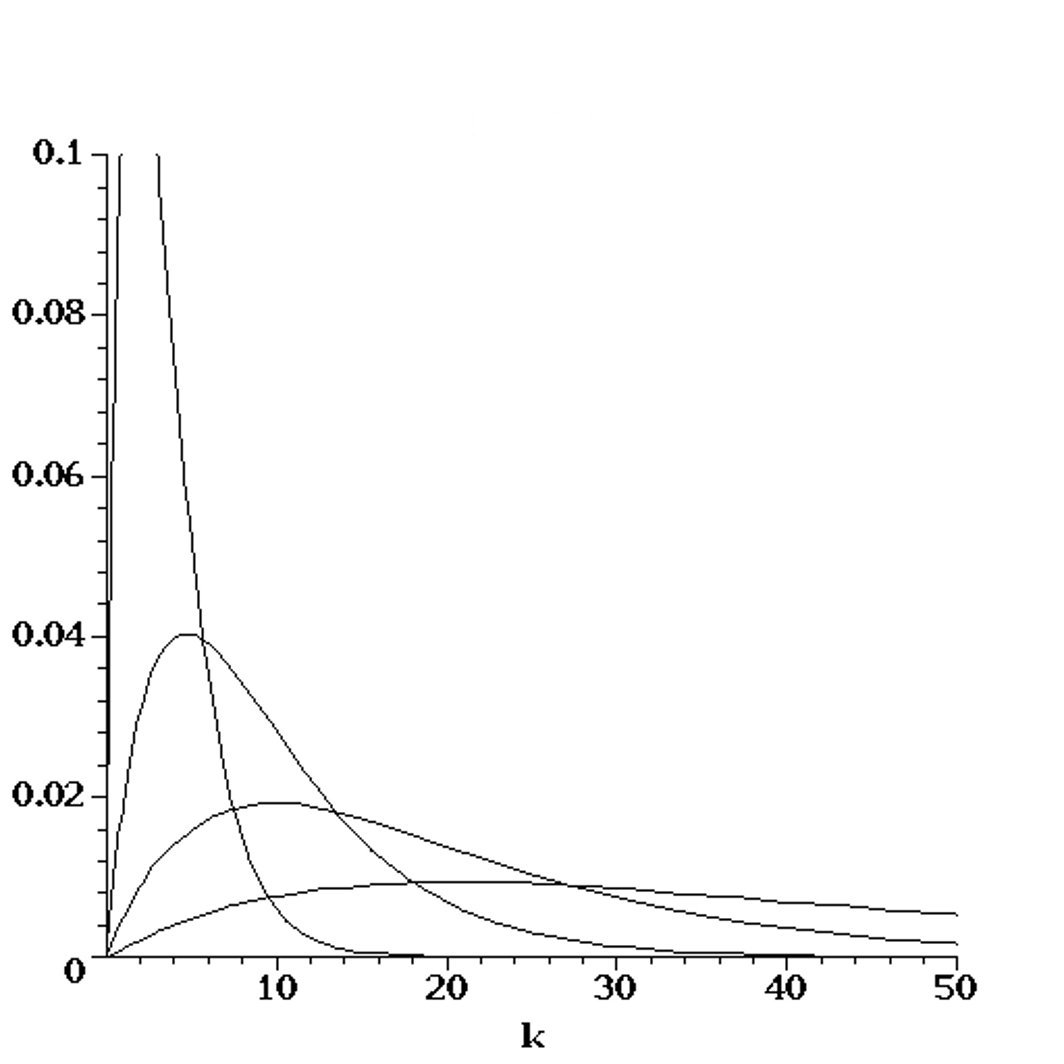
\includegraphics[width=0.35\textwidth]{figures/ch1_7_biais.jpeg}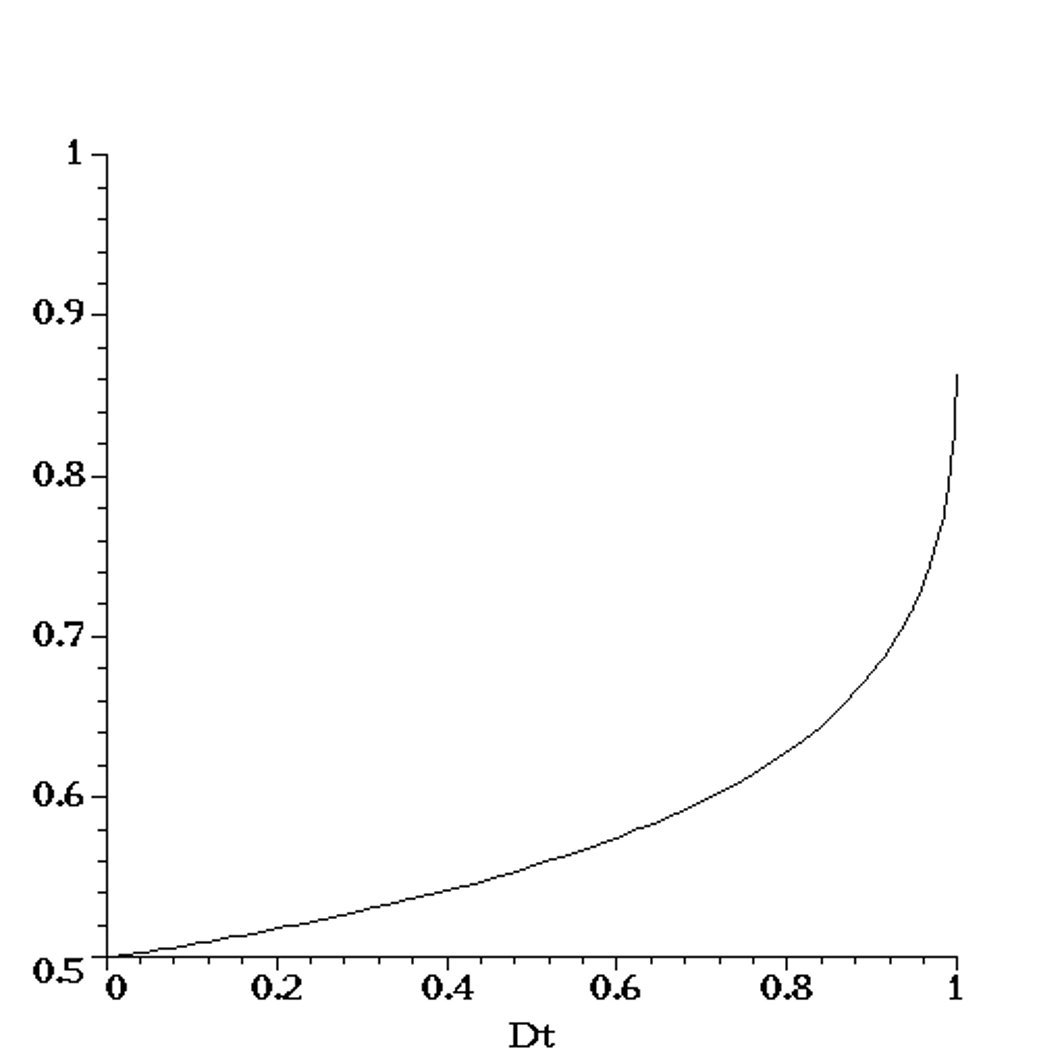
\includegraphics[width=0.35\textwidth]{figures/ch1_7_integralbiais.jpeg}\end{center}
\caption{{\em \`A gauche}: Le profil temporel normalisé du biais de calcul entre le schéma continu et son approximation discrète pour $\Delta t / \tau_j = [0.05, 0.1, 0.2, 0.5]$ en partant de la courbe la plus plate à la plus pointue .
{\em \`A droite}: L'intégral du biais le long de la trajectoire en fonction de $Dt=\Delta t / \tau_j$, en explicitant que l'écart systématique cumulatif n'est jamais négligeable, même pour des valeurs très faibles du terme de fuite, alors qu'il diverge pour les valeurs importantes. Voir le texte pour plus de détails.}
\label{fig: euler-error} 
\end{figure} 


Dans un tel cas, le schéma continu et son approximation discrète convergent vers le même point fixe en partant de la même valeur initiale, mais pas selon la même trajectoire. Plus précisément, le biais dans une direction propre de la matrice $ {W} $ est proportionnel à $ V_j (0) - I_j \, \tau_j$, où $ 1 / \tau_j $ est la valeur propre (qui correspond au terme de fuite) dans cette direction, et suit le profil d'une exponentielle double (fonction de $\Delta t / \tau_j$), comme illustré dans la figure~\ref{fig: euler-error}. Autrement dit, plus $\Delta t / \tau_j  \in [0, 1 [$ (les bornes correspondant à l'intervalle de convergence) est élevé, plus l'écart entre les deux schémas (continu et discontinu) est important, mais moins la durée du biais (la durée pendant laquelle le biais est non nul) est importante.\\

Il s'agit d'un résultat contre-intuitif et très important de noter que les grandes valeurs du terme de fuite (constantes de temps faibles) accélèrent la convergence. Mais il reste l'inconvénient de générer des erreurs importantes au cours des premières itérations. Même dans un tel cas très simple, au début de la trajectoire, l'approximation discrète du système dynamique continu peut très bien ne pas converger vers l'attracteur attendu du système continu (voir la courbe discontinue correspondant à $\Delta t / \tau_j = 0.05$ fig.~\ref{fig: euler-error}), mais vers un autre comme on l'observe dans \cite {Rougier:2009}.\\

Dans le cas plus général o\`u le terme de fuite, les poids ou les entrées varient avec le temps, les résultats précédents se généralisent compte tenu du fait que le terme de fuite est borné. Dans le cas non-linéaire, les résultats précédents se généralisent aussi en délimitant la fonction non-linéaire $\sigma_ {j}$ par la fonction linéaire correspondante de pente maximale (voir, \cite {Cessac:2007}) pour un examen de ces outils). \\%Plus précisément, si le système est hyperbolique, la même condition s'applique sur la Jacobienne du système à tout moment et pour toute valeur.\\

En conséquence, nous apprenons de cette courte analyse que, généralement, même si le schéma continu et le schéma discontinu peuvent converger vers le même point fixe, ils ne convergent pas selon la même trajectoire. Dans tous les cas, l'écart systématique cumulatif n'est jamais négligeable.\\
%%%%%%%%%%%%%%%%%%%%%%%%%%%%%%%%%%%%%%%%%%%%%%%%%%%%%%%%
%%%%%%%%%%%%%%%%%%%%%%%%%%%%%%%%%%%%%%%%%%%%%%%%%%%%%%%%%%%%%%%%%%%%%%%%%%%%%%%%%%%%%%%%%%%%%%%%%%%%%%%%%%%%%%%%%%%%%%%%%%%%%%%%%%%%%%%%%%%%%%%%%%%%%%

Il en résulte donc que lors de la simulation d'un système à temps continu régie par une équation différentielle, le choix du schéma de discrétisation détermine la précision des trajectoires de son évolution (la précision de la dynamique) même si l'état final est souvent conservé. Le problème est que plus on essaye d'approcher le schéma de discrétisation du schéma continu, plus la mise en oeuvre est compliquée et couteuse en termes de ressources de calcul. Donc c'est l'objectif des travaux de simulation qui impose le niveau de détail et de précision à choisir pour maximiser le rapport qualité/prix.

%%%%%%%%%%%%%%%%%%%%%%%%%%%%%%%%%%%%%%%%%%%%%%%%%%%%%%%%%%%%%%%%%%%%%%%%%%%%%%%%%%%%%%%%%%%%%%%%%%%%%%%%%%%%%%%%%%%%%%%%%%%%%%%%%%%%%%%%%%%%%%%%%%%%
\section{Calcul distribué: A-t-on vraiment besoin d'une horloge centrale?}

Quelle que soit la méthode numérique utilisée pour résoudre les équations différentielles qui décrivent l'évolution du système, il est supposé implicitement qu'il y a une horloge centrale pour synchroniser les calculs. Par exemple, pour calculer les variables du modèle à l'instant $t$, les méthodes explicites utilisent l'information disponible sur toutes les variables du modèle à l'instant $t-\Delta t$. La connaissance de quelle unité a été mise à jour à tel instant $V(i)$ doit donc être centralisée pour pouvoir donner le signal permettant de passer à la prochaine étape $V(i+1)$.\\

Quelles sont les conséquences? Au niveau informatique, cela signifie que si nous utilisons une architecture multi-processeurs, les processeurs qui terminent leur tâche en premier doivent attendre à ne rien faire, jusqu'à ce que les autres finissent. Au niveau du système dynamique, ces mises à jour régulières peuvent induire des mécanismes de synchronisation parasites. En effet, des simulations ont montré que des états synchronisés peuvent appraître rapidement dans des réseaux de neurones impulsionnels réciproquement couplés \cite{Hopfield:1995}. Au niveau de la modélisation biologique, si l'on suppose l'existence d'une horloge globale universelle, qui est une approximation raisonnable pour les petits systèmes dynamiques, il est moins évident lorsque l'on considère plusieurs cartes corticales en interaction avec des délais de transmission complexes.\\

Mais puisque la caractéristique de base des réseaux de neurones est de pouvoir assurer un calcul distribué (chaque neurone détient une partie de l'information), il est assez contre-intuitif de s'appuyer implicitement sur une telle horloge centrale. Dans ce contexte, nous tenons à étudier dans quelle mesure nous pouvons éliminer cette horloge centrale et mettre en oeuvre un calcul plutôt \textit{asynchrone} dans le cadre des DNF, ce qui a déjà été étudié dans le cas des automates cellulaires \cite{Fates:2005, Fates:2008, Garcia:2006, Barret:1999, Robert:1994} et les calculs parallèles\cite{Bertsekas:1991, Bertsekas:1997} où les différents niveaux de synchronie numérique ont été pris en compte.\\ 


\subsection{De l'\'evaluation synchrone vers l'\'evaluation asynchrone }

Le calcul synchrone se réfère à la méthode numérique standard utilisée pour résoudre un ensemble d'équations différentielles \textit{ordinaires}. Après avoir choisi une résolution temporelle $ \Delta t $, une valeur $ V_i (t + \Delta t)$ est évaluée en fonction de $ V_i (t) $ et $ \Delta V_i (t) / \Delta t $ en utilisant une des nombreuses méthodes implicites ou explicites disponibles (Euler, Runge-Kutta, etc.).\\ 

Puisque n'importe quelle valeur $ V_i (t + \Delta t) $ dépend de la valeur de $V_j$ à des moments antérieurs et peut notamment dépendre de $ V_j (t + \Delta t)$, il est important de mettre à jour $ V_i (t)$ une fois que toutes les valeurs $ V_j (t + \Delta t) $ sont connues. En d'autres termes, chaque unité calcule son état suivant sans l'afficher, puis toutes les unités changent leur état actuel ($ V_i (t) $) en ($ V_i (t + \Delta t $) simultanément. Cela nécessite donc un contrôle centralisé signalant les unités qui sont autorisées à mettre à jour ``publiquement'' leur état. Même si tous les états ne sont pas modifiés à chaque étape, comme par exemple avec la méthode de Gauss-Seidel \cite {Bertsekas:1991}, l'horloge centrale est toujours nécessaire (parce que nous devons nous assurer que chaque unité a été mise à jour exactement une fois), donc le calcul reste macroscopiquement synchrone dans ce sens. \\

Un système \textit{totalement asynchrone} implique donc de contourner une telle horloge globale et de laisser le système fonctionner sous un contrôle entièrement distribué. D'un point de vue informatique, cela signifierait que chaque processeur est une unité indépendante avec une notion locale de temps et est donc mis à jour séparément. D'un point de vue biologique, cela refléterait plusieurs aspects:\\

\begin {itemize}
\item Une asynchronie entre les éléments à mettre à jour générée par les délais de communication liés aux durées de traitement et de transmission.\\

\item Une asynchronie adaptative, c'est à dire le fait qu'une unité adapte l'évaluation de son état: plus sa valeur est stable, moins de mises à jour seront faites. Ici l'asynchronisme est utilisé comme un outil computationnel.\\

\item Des événements mésoscopiques comme le changement soudain d'activité et l'influence des événements extérieurs. Ici l'asynchronisme devient liée à certaines fonctionnalités du système.\\
\end {itemize}

A ce niveau de modélisation, où le traitement de l'information est un aspect clé du calcul neuronal, nous pouvons avoir des temps d'exécution différents et des unités qui ne sont pas sensées attendre que les autres finissent leur traitement. En outre, les délais de transmission contribuent à désynchroniser les informations échangées. Les deux phénomènes sont à prendre en compte dans un paradigme \textit{totalement asynchrone}. En d'autres termes, l'asynchronisme n'est pas seulement un problème d'implémentation, il est également un problème de modélisation.\\

\subsection{Le paradigme de calcul asynchrone}\label{paradigme}

\cite {Mitra:1987} présente un travail important sur l'informatique asynchrone qui aborde le sujet un niveau très général. Son approche originale s'inspire de l'ouvrage de \cite{Chazan:1969} qui propose et analyse des algorithmes asynchrones à utiliser dans des processeurs parallèles, entre autres pour la résolution de systèmes d'équations linéaires, non linéaires ou d'équations différentielles. Ces deux références proposent un certain nombre de résultats de convergence. En suivant les travaux de Mitra \cite{Mitra:1987}, nous proposons le paradigme de calcul asynchrone suivant: le calcul est divisé en unités locales qui envoient leur résultat vers les autres unités dès que leur calcul est achevé. A chaque unité d'indice $i$ correspond une approximation de l'équation~(\ref{eq: DNF-discret}).\\

Plus précisément, à un moment donné d'échantillonnage d'indice $k$, seul un sous-ensemble d'unités choisies arbitrairement $S(k)$ est évalué. $S(k)$ définit un sous-ensemble de $\{1,2, ..., n \}$ désignant les indices d'unités à être mis à jour à $ t = k \Delta t$ (la $ k ^ {eme} $ mise à jour).\\

Ce schéma très simple peut rendre compte de l'évaluation synchrone ($ S (k) = \{1,2, ..., n \} $, toutes les unités sont mises à jour simultanément), de l'évaluation en série de Gauss-Seidel ($S(k)$ ne contient qu'un seul indice à chaque mise à jour, chaque unité ne peut pas être mise à jour plus d'une fois avant que le système entier soit mis à jour), ainsi que les autres régimes asynchrones (par exemple, $S(k)$ contient des indices de plusieurs unités tirées au hasard, avec ou sans remise en termes de probabilité), etc.\\

En outre, chaque connexion entre deux unités $i$ et $j$ peut induire un retard d'exécution $ \Delta_ {ij}(t) $ constant ou variable: l'information sur l'état $V_j(t)$ est disponible à l'unité $i$ seulement après un tel retard. $\Delta_{ij}(t)$ peut correspondre à plusieurs $\Delta T$.\\

Un point clé est le suivant: chaque unité ne calcule pas $V_i (t)$ étant données certaines valeurs de mises à jour, mais calcule une approximation de la trajectoire entière $ \{V_i (t), 0 \leq t \} $, sachant une certaine connaissance tardive sur les unités qui lui sont connectées $ \{\hat {V} _j (t), 0 \leq t <t_ {ij} (t), j \in M ​​\} $:\\ 

\begin {itemize}
\item Dans un premier temps, chaque unité ne connaît que sa valeur initiale $ V_i (0) $, donnée a priori, et doit spécifier une première valeur des trajectoires des unités connectées (par exemple, en supposant que $ V_j (t) \simeq V_j (0) $, comme la meilleur hypothèse lorsque rien n'est calculé).

\item Puis, chaque unité commence à estimer une approximation d'une partie de sa trajectoire, jusqu'à un certain temps $t_i$: $ \{V_i (t), 0 \leq t <t_i \} $, et communique cette information de manière asynchrone à d'autres unités.

\item Quand une certaine connaissance (information) est reçue par une unité, celle-ci met à jour sa propre approximation et ainsi de suite.\\
\end {itemize}

Donc ce paradigme exige seulement que:

\begin {itemize}
\item[$(i)$]  les valeurs initiales correspondent aux valeurs initiales attendues et ceci pour toutes les unités.
\item[$(ii)$] chaque unité doit pouvoir résoudre le problème spécifié dans~(\ref{eq: DNF-discret}) (calculer une approximation convergente de la trajectoire de la solution étant donnée la valeur initiale). 
\end {itemize}

\subsection{Convergence des algorithmes asynchrones}\label{convergence}

Examinons maintenant la question de la convergence des algorithmes asynchrones. Ici nous allons discuter le cas le plus général puis fournir des résultats plus précis dans un cas particulier de DNF.\\

Le modèle de calcul asynchrone utilisé est décrit dans la section~\ref{paradigme}: à un pas d'échantillonnage d'indice $k$, seul un sous-ensemble d'unités choisies arbitrairement $S(k)$ est évalué, par conséquent, il n'y a {\em aucune restriction} sur le type du modèle asynchrone.\\

Chaque unité d'indice $i$ est mise en oeuvre par une tâche $T_i$, qui calcule la solution unique du problème. Par conséquent, chaque étape de calcul résout le système linéaire local compte tenu des meilleures connaissances disponibles concernant les autres unités. La question clé est de savoir si un tel mécanisme résout itérativement le problème général non-linéaire. Une réponse positive, détaillée ici, fut donnée par \cite{Mitra:1987}.\\

Supposons que nous sommes dans un {\em cadre asynchrone borné}, c'est à dire deux principales hypothèses sont nécessaires:\\

\begin {itemize}
\item [$\bullet$]{\em retards bornés}. Les retards devraient être bornés par un nombre fini constant et uniforme $\Delta_{ij} \le D < +\infty $. 
\item [$\bullet$] {\em condition anti-famine}. Il y a une limite maximale uniforme $B$, entre deux mises à jour pour une unité donnée. Chaque unité doit fournir une mise à jour au moins une fois pendant tout intervalle de temps de longueur $B$. Ce qui garantit qu'il n'y a pas d'unités ``mortes'' qui ne se mettent jamais à jour.\\
\end {itemize}


Différentes versions de ces hypothèses ont été considérées comme nécessaires à la convergence des algorithmes de calcul asynchrone, comme dans \cite{Chazan:1969}. C'est ainsi qu'en ajoutant certaines conditions supplémentaires sur les équations différentielles du système (spécialement le terme de fuite), la convergence uniforme\footnote{La convergence uniforme d'une suite de fonctions $(f_n)_{n \in N}$ définies de I dans R est une forme de convergence plus exigeante que la convergence simple. On dit que cette suite converge uniformément vers une fornction $f$ définie sur $I$ si à tout $\epsilon>0$ on peut faire correspondre un entier $P(\epsilon)$, indépendant de $x\in I$, tel que pour tout $n>P(\epsilon)$ on a : $\vert f_n(x)-f(x)\vert<\epsilon$ \cite{Pisot:1966}} géométrique\footnote{On dit qu'une suite ($U_n$) converge (au moins) géométriquement vers 0 si elle est dominée par une suite géométrique ($k^n$) avec $0 < k < 1$. Le théorème suivant est essentiel pour assurer qu'une convergence est géométrique: Théorème d'Alembert. Soit ($U_n$) une suite de nombres positifs. On suppose que le rapport $\frac{U_{n+1}}{U_n}$ tend vers un nombre $k$ avec $0 < k < 1$. Alors, la suite ($U_n$) converge vers 0 géométriquement et plus précisément, si $\epsilon$ est un nombre $> 0$ qui vérifie $k +\epsilon< 1$, la suite est dominée par $(k + \epsilon)^n$. (On parle, dans ce cas, de convergence géométrique de rapport k.)} est prouvée. Examinons avec précision ce résultat.\\

Prenons ${W}$ la matrice de poids définie dans~(\ref {eq: def-W}) dans le cas sans délais de transmission et quand $\sigma_j(u) = u $. Si la non-linéarité $ \sigma_j (u) $ est présente, en utilisant les inégalités différentielles, le système non-linéaire doit être délimité par un système linéaire de poids $W'$ (voir \cite {Mitra:1987} pour plus de détails). Malgré les difficultés techniques, l'idée sous-jacente est très simple: le poids doit être multiplié en quelque sorte par la plus haute pente de la non-linéarité, c'est à dire $  W'_{ijk} \simeq \sigma_j '(0) \, W_{ijk } $ dans le cas d'une sigmoïde. Donc le résultat suivant peut être généralisé.\\

Sur cette base, si nous nous référons aux travaux de Mitra, notre équation différentielle est un cas particulier du cadre proposé \footnote {Il correspond à l'équation~(6.7i) de \cite{Mitra:1987} ($\frac{d}{dt}x(t)+Dx(t)=Bx(t)+u(t)$ o\`u $D$ et $B$ sont indépendantes de t et $x$ et $u$ sont des éléments de $R^{n}$), avec $ {D} = {I} $ (matrice identité) et $ {B} = {W} $.}. L'application de la proposition 2 de cet article: {\em la convergence uniforme géométrique dans le mode asynchrone se produit lorsque, dans notre cas, $ {I} - |{ W}|$ est une M-matrice} (une matrice dont les entrées hors-diagonales sont inférieures ou égales à zéro, avec des valeurs propres dont les parties réelles sont positives).\\

Dans les DNF, les noyaux sont souvent isotropes, $ {W} $ est une matrice symétrique positive, donc diagonalisable et avec des valeurs propres positives. D'o\`u ${I} - |{W}|$ est une M-matrice tant que ces valeurs propres sont inférieures à $1$, cette condition étant exactement ce qui est nécessaire pour que le système soit numériquement stable \cite{Alexandre:2009}.\\

Dans le cas général des poids anisotropes, la condition ``$I - |W|$ est une M-matrice'' se vérifie numériquement en se basant sur les standards de l'algèbre linéaire (calcul du déterminant, diagonalisation...). En outre, puisque le terme de fuite $L_i $ doit être ``assez élevé'', il est possible de concevoir aisément un mécanisme algorithmique qui ajuste les valeurs de ${W}$ jusqu'à ce que la condition M-matrice soit vérifiée.\\

En conséquence, on obtient un résultat pertinent très précis. La convergence de calcul asynchrone dans un tel réseau de neurones est garantie et le rapport (taux) de convergence moyen (par mise à jour) n'est pas inférieur à:

%%
\begin{align}
\label{eq: convergence}
\frac{1}{\tau_{\min}} \leq \frac{1}{D + B}
\end{align}
%%
où $ 1/ \tau_{\min} $ est le rayon spectral\footnote{Soit A une matrice carrée à coefficients complexes. On appelle rayon spectral le plus grand module des valeurs propres de A.} de $ {W} $, c'est à dire, la plus grande valeur propre (positive ici) correspondant donc à la plus petite valeur du terme de fuite. $D$ est le délai maximal et $B$ est la pseudo-période maximale (période pendant laquelle chaque unité est mise à jour au moins une fois).\\

Donc le problème principal, même si le système est fini et le temps est discret, n'est pas seulement d'assurer la convergence vers un état stable (ce qu'on obtient lorsque le système est contractant), mais de garantir que le calcul va faire converger le système vers le résultat attendu. Dans le cas non-linéaire, Mitra suppose que les fonctions non-linéaires sont lipschitziennes\footnote{Soit $I$ un intervalle de $R$, $f$ une fonction de $I$ dans $R$. On dit que f est lipschitzienne de rapport $k>0$ si pour tout $x,y$ de $I$: $|f(x)-f(y)|\le k|x-y|$} et bornées par une fonction linéaire contractante, pour obtenir le même résultat. Dans notre cas, cela signifie que la fonction de transfert non-linéaire $\sigma$ ne peut pas être une fonction de Heaviside, mais tout profil continu de sigmoïde est commode. \\ %\footnote {Plus précisément, nous avons soigneusement vérifié que les fonctions sigmoïdes usuelles (fonctions strictement croissantes régulières de $ {\cal R} \rightarrow [0, 1] $) vérifient les hypothèses N1, N2 et N3 à partir de \cite {Mitra:1987}. }.\\

Dans le cas non-linéaire, plusieurs points fixes sont en effet possibles. Un régime asynchrone numérique standard ``pas par pas'' peut faire dévier la trajectoire vers un bassin d'attraction différent de celui obtenu en régime synchrone (et donc une autre «réponse» au même stimulus). Ici, puisque l'itération ne se fait pas ``étape par étape'', mais le rapprochement de la trajectoire entière est recalculée à chaque étape, nous sommes dans une situation où la convergence vers la solution ``continue'' est obtenue, au prix de l'hypothèse assez forte sur le terme de fuite (suffisamment important pour permettre d'absorber les oscillations au début de la trajectoire). Ce résultat est à prendre avec précaution au niveau numérique, car les erreurs d'arrondi parasites peuvent encore induire des déviations de trajectoire.\\

\subsubsection{Convergence quand les valeurs sont discrètes}

Dans la communauté d'analyse numérique, le livre de référence dans le contexte à la fois continu et discret est celui de Bertsekas et Tsitsiklis, chapitres 6 et 7 \cite{Bertsekas:1997}. Il présente quelques algorithmes et donne des conditions suffisantes pour la convergence pour des problèmes non-linéaires et des conditions nécessaires pour des problèmes linéaires.\\

Dans le cas particulier des systèmes dynamiques discrets, sans retards de transmission, le résultat principal présenté dans \cite{Robert:1994, Bahi:2002} est que si un système est pseudo-périodique, il converge au plus au bout de $N$ pseudo-périodes, $N$ étant le nombre total des unités dans le système. Donc, avec seulement $N$ points de synchronisation (date à laquelle toutes les unités du systèmes ont été mises à jour au moins une fois), la convergence du système est garantie. Mais lorsque nous introduisons les délais de transmission et les variables continues, une telle hypothèse n'est plus valable et n'assure donc pas la convergence.\\

\subsubsection{Un exemple illustratif}

Prenons par exemple un réseau à deux couches, une couche d'entrée à valeurs constantes et une couche de sortie, chaque couche étant de taille $ N \times N $ unités. Chaque unité d'indice $i$ de la couche de sortie reçoit une entrée $I_{i}$ de la couche d'entrée selon un champ récepteur gaussien.\\

Nous supposons qu'il n'y ait ni connexion latérale, ni rétroaction dans la couche d'entrée. Dans la couche de sortie, les connexions latérales sont excitatrices, diminuant avec la distance et l'entrée est inhibitrice (le profil de connectivité inverse est également approprié). Cela signifie que chaque neurone (unité) dans la couche de sortie est excité par ses voisins et inhibé par les neurones d'entrée qui sont dans son champ récepteur. L'activité résultante dans la carte de sortie est une différence de gaussiennes (un profil très utilisé dans les réseaux de neurones dynamiques).\\

Donc, dans ce cas, pour chaque couche de $M = N \times N $ unités, l'équation~(\ref {eq: DNF-discret}) s'écrit avec des poids $W_{i = (u, v) \, j = (u ', v') \, d}$, indexés en fonction de la géométrie 2D du réseau et $ V_ {i} $ représente le potentiel de membrane, $ W_{ijd} $ est un tenseur symétrique positif dans ce cas, et $ I_ {i} $ est l'entrée constante provenant de la projection de la couche d'entrée. Une instanciation, sans retards dans les poids $(d=0)$, serait de choisir:

\begin{align}
W_{ij0} = a_+ \, e^{-\frac{|i - j|^2}{v_+^2}} -  a_- \, e^{-\frac{|i - j|^2}{v_-^2}} \notag
\end{align}
%%
puis en tant que corollaire des travaux présentés dans \cite{Alexandre:2009}, nous pouvons affirmer que:
%%
\begin{align}
\frac{1}{\tau_{\min}} \simeq \sqrt{\pi} \, (a_+ \, v_+ - a_- \, v_-) \notag
\end{align}

l'approximation étant de négliger l'effet de bord de la carte 2D correspondante. Puis en combinant ce résultat avec~(\ref {eq: convergence}), nous avons une borne limite concrète de la convergence asynchrone.\\

%Bien que ce résultat a été calculé en forme fermée afin de pouvoir utiliser ~ (\ref {eq: la convergence}) dans ce cas précis, il est important de noter que dans un cas plus général, la seule exigence est de calculer le rayon spectral de $ {\bf W} $, ce qui est numériquement facile à mettre en oeuvre.\\
Donc pour tous les schémas généraux d'évaluation asynchrone, si l'attracteur du DNF est un point fixe, les délais de transmission sont bornés et le critère anti-famine est validé, alors la convergence uniforme géométrique est garantie. On peut donc considérer le dilemme de l'évaluation synchrone/asynchrone dans la simulation des DNF comme résolu dans un tel contexte.\\




\subsubsection{L'approche événementielle: Un exemple d'implémentation}

Considérons un dernier aspect du calcul asynchrone, c'est à dire pas le fait que nous voulons simuler un système continu de façon asynchrone, mais le fait que nous voulons simuler un système {\em intrinsèquement asynchrone} avec un dispositif de calcul séquentiel ou distribué. Cela couvre deux aspects fondamentaux. D'une part, chaque unité dispose d'une horloge locale. Cela signifie qu'il y a des retards, de valeurs imprévisibles entre les unités. D'autre part, l'information est définie par deux attributs, une valeur et le moment où cette valeur a été délivrée. En d'autres termes, l'information est définie à travers des événements temporels.\\

Dans un travail récent \cite {Rougier:2006}, un modèle computationnel a été conçu, en utilisant uniquement les connexions locales et une inhibition globale. 
Nous avons ré-implémenté ce mécanisme en utilisant un régime asynchrone mis en oeuvre avec un noyau minimal de simulation événementielle \footnote {code disponible à {\tt http://enas.gforge.inria.fr}, {\tt Enas} étant un simulateur à grande échelle de populations de neurones événementiels.}, la garantie de convergence étant donnée par la discussion précédente.Le schéma de calcul événementiel (\textit{event-driven}) a été principalement développé pour les modèles de neurones à spikes\footnote {Voir \cite {Gerstner:2002} pour une introduction et \cite {Cessac:2008, Cessac:2010} pour une analyse théorique récente et une discussion générale en lien avec ces aspects}.  L'outil de simulation dédié est un simulateur évènementiel tel que proposé par \cite{Rochel:2003} dans le cadre de la spécification des systèmes à événements discrets (DEVS, \textit{discret event system specification}) (\cite {Brette:2007, Cessac:2009}). \\

Très concrètement, chaque unité doit fournir une estimation de la date la plus proche du prochain événement (décharge). En plus, la mise à jour de l'état interne de l'unité doit aussi être définie. Les DEVS permettent de montrer que, compte tenu de cette spécification, un système totalement asynchrone peut être simulé, en utilisant un calendrier avec une file d'attente simple d'événements, sur n'importe quel appareil (voir, par exemple, \cite{Cessac:2009} pour plus de détails).\\% Cela permet non seulement de simuler des calculs asynchrones sur un système centralisé, mais aussi de mélanger les deux types de mises en oeuvre.\\

La figure~\ref{fig: bump} montre le résultat de la simulation numérique, avec l'heuristique supposant que la période d'échantillonnage locale est à peu près proportionnelle à la variation de la valeur d'état (principe de parcimonie \footnote{ Le principe de parcimonie (o\`u ``rasoir d'Occam'') est un principe scientifique fondamental consistant à utiliser le minimum de causes élémentaires pour montrer la vraisemblance d'une hypothèse ou expliquer un phénomène \cite{Fernandez:2010}}), avec une grande robustesse à l'égard des paramètres connexes (la modification des paradigmes asynchrones modifie les valeurs transitoires, influence légèrement la vitesse de convergence, mais ne modifie pas le résultat final). Sur ​​cet exemple de simulation numérique, la vraie solution a été approchée avec précision et plusieurs fonctions qualitatives d'entrée/sortie du DNF (filtrage de la forme de la bulle d'activité de sortie, sélection d'une bulle de sortie parmi plusieurs bulles d'entrée, suivie d'une bulle en mouvement...) ont été reproduites (voir \cite {Alexandre:2009} pour plus de détails). \\

Sachant que l'équation~(\ref{eq: convergence}) est vérifiée, le calcul est garanti dans tous les cas observés. Et la convergence a été obtenue toujours vers la solution obtenue dans le cas synchrone, le biais étant négligeable. Des expériences préliminaires tendent à montrer que l'échec de convergence est observé lorsque la borne est largement dépassée. En outre, nous avons observé que le nombre de mises à jour pour arriver à la convergence est toujours plus élevé dans le cas asynchrone .\\

Afin de fournir une étude préliminaire, nous avons considéré un mécanisme ``parcimonieux'' correspondant au résultat de la figure ~\ref{fig: bump} (tous les paramètres sont fixés en fonction de \cite{Alexandre:2009}).\\
%\\facteur 5, dans notre cas), ceci reste à examiner.\\

\begin{figure}[htbp]
\begin{center}
\begin{tabular}{|c|c|}
\hline
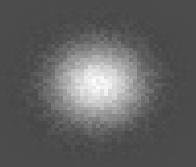
\includegraphics[width=0.25\textwidth,height=0.25\textwidth]{figures/ch1_8_intermediateAsyn.jpeg} & 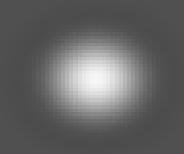
\includegraphics[width=0.25\textwidth,height=0.25\textwidth]{figures/ch1_8_finalAsyn.jpeg}\\
\hline
\end{tabular}
\end{center}

 \caption{Un exemple de traitement asynchrone des cartes neuronales (implémentation évènementielle), en appliquant les critères de convergence dérivés ici. Nous avons vérifié numériquement la conjecture que les résultats actuels s'appliquent lorsque l'évaluation est asynchrone. {\em Vue gauche}: résultat intermédiaire, la randomisation est visible. {\em Vue droite}: résultat final, après la convergence. Cela a été expérimenté sur un DNF $ 128 \times 128 $ avec un profil de connectivité latérale en différence de Gaussiennes, en utilisant les mêmes valeurs dans les cas synchrones et asynchrones. Deux paradigmes asynchrones ont été expérimentées: (1) En utilisant les temps de mise à jour aléatoires uniformément établis dans un intervalle compatible avec les conditions de Mitra. (2) Un mécanisme ``parcimonieux'' , voir le texte pour plus de détails.}

\label{fig: bump} 
\end{figure}

Ici les dates de mises à jour $ \Delta_ {ij} $ ont diminué comme une fonction linéaire de la variabilité de la valeur de l'état ​​$ \Delta V_i$ (mise à jour rapide pour les valeurs qui varient rapidement),
et nous avons simplement choisi $ \Delta_{ij} = \Delta_{max } \, (1 - \Delta V_i / \Delta V_ {max}) $, pour obtenir des retards entre $ 1$ et $ 10 $ périodes d'échantillonnage. Cela a considérablement diminué le nombre d'étapes (mieux que dans le paradigme synchrone), une étude précise sera une perspective de ce travail.\\

\section{Discussion}


Dans ce chapitre nous avons examiné les quatre aspects importants du cadre de modélisation:
\begin{enumerate}
\item Le neurone comme unité de base et règle de calcul locale.
\item L'approche connexionniste et la plasticité synaptique.
\item L'intégration numérique et les problèmes de discrétisation dans le cadre particulier de la CNFT, en particulier l'étude du biais entre une trajectoire continue et son approximation discrétisée au cours du temps.
\item L'utilisation de mécanismes synchrones/asynchrones à la fois au niveau de la modélisation et au niveau de l'implémentation dans une approche de calcul distribué, en particulier les garanties de convergence de l'évaluation asynchrone vers la solution prévue.\\
\end{enumerate}

Nous nous sommes concentrés sur le 3{\ieme} et le 4{\ieme} point en nous plaçant dans le cadre des DNF. Nous avons montré que des méthodes d'évaluation asynchrones peuvent être efficacement utilisées pour la simulation dynamique des champs de neurones. Dès que des hypothèses raisonnables sont vérifiées, la convergence rapide et la faiblesse du biais sont garantis. En retour, comme nous l'avons expliqué dans la section \ref{convergence}, la théorie des champs de neurones dynamiques fournit un bon terrain pour l'étude des systèmes d'évaluation asynchrone. Par exemple, dans \cite {Rougier:2006}, il a été démontré (numériquement) que cette méthode d'évaluation asynchrone conduit à de nouvelles solutions stables qui sont fonctionnellement différentes de celles obtenues par le schéma continu. Lorsqu'on présente deux stimuli identiques à deux endroits différents, le champ est capable de se stabiliser sur l'un ou l'autre des deux stimuli et donc briser la symétrie du système. Toutefois, on peut montrer facilement que ce nouvel état très stable peut ne pas être une solution de l'équation continue du champ. Quel est donc la pertinence d'une telle description continue si l'on veut l'évaluer en utilisant les équations numériques asynchrones? Idéalement, nous aimerions pouvoir disposer d'une description asynchrone continue équivalente mais malheureusement, ce n'est pas encore le cas dans le domaine des mathématiques. Nous devrions alors prendre des précautions supplémentaires lors de la description d'un système décrit par des équations continues et la question suivante se pose : est ce qu'on simule vraiment ce que nous avons annoncé dans la définition du système? En particulier, au niveau de la modélisation mésoscopique, il peut être intéressant d'utiliser un paradigme basé sur les événements au lieu d'une horloge centrale, car il s'agit d'un paradigme qui prend en considération le fait que non seulement le traitement mais aussi le calendrier de mises à jour sont entièrement distribués. \\

D'un point de vue plus cognitif, cette étude révèle la présence implicite d'une horloge centrale dans un certain nombre de modèles et donc la présence implicite d'un grand superviseur pour orchestrer l'activité globale du modèle. Une future étape du travail sera l'utilisation d'un cadre basé sur le codage événementiel où il est possible de contrôler, à la fois, la valeur et le {\em temps} de mise à jour de cette valeur. Il est possible de simuler dans un tel cadre tous les régimes asynchrones possibles (schéma périodique, relaxation chaotique, etc. \cite {Chazan:1969, Amitai:1993}). Une telle plate-forme permet donc de déterminer quel schéma numérique asynchrone est pertinent pour une modélisation temporelle donnée, ouvrant la voie pour étudier concrètement au niveau mésoscopique, le temps de calcul. En fait, si les limites examinées dans le présent document garantissent la convergence, rien ne peut a priori être déclaré sur les performances, ou l'émergence de phénomènes transitoires, etc.\\

Enfin, l'évaluation asynchrone a l'avantage d'être un schéma de calcul qui s'approche plus de la réalité du système nerveux qui s'articule autour d'unités élémentaires indépendantes. En plus, ce paradigme est en faveur de l'implémentation informatique distribuée fortement souhaitée d'un point de vue informatique. Mais comme on peut le constater dans ce chapitre, la mise en oeuvre d'un tel schéma de calcul rend à la fois la modélisation et l'implémentation plus compliquées. C'est pourquoi nous avons choisi le schéma d'évaluation synchrone dans les modèles que nous allons proposer par la suite puisqu'on va se concentrer plus sur les flux d'information et les propriétés émergentes des dynamiques locales. De plus, puisqu'on se place à l'échelle mésoscopique en s'intéressant à la modélisation des structures corticales et sous-corticales nous avons adopté le codage fréquentiel. Le codage impulsionnel étant plus adapté à la modélisation à l'échelle du neurone, l'utiliser pour des modèles d'interactions de plusieurs populations de neurones nécessite plus de puissance de calcul. De plus si les propriétés temporelles des trains de spikes (dates, phases, synchronie...) ne sont pas examinées et seule la fréquence moyenne de décharge est évaluée, il n'est pas nécessaire de passer par une modélisation à spikes. Enfin, tous les mécanismes présentés dans nos modèles ont été simulés en utilisant la méthode d'Euler qui est la moins coûteuse en termes de calcul et la plus simple. En utilisant cette méthode, nous avons conscience des erreurs de simulation par rapport au système à temps continu et nous optons pour des temps d'échantillonnage faibles permettant de conserver les propriétés émergentes des interactions.



%\setcounter{Chapter}{1}
\DontNumberThisInToc
\DontFrameThisInToc
\glsresetall
\ChapterNumberCitation{Le Système Visuo-moteur}{Perception is not something that happens to us, or in us, it is something we do.}{ N. Alva, Action in Perception, 2006}{10cm}
\Citation {During visual search, the brain
performs a sophisticated deployment
of eye movements (\protect\textit{saccadic actions})
to gather information to subserve
perceptual judgments}
{P.E Miguel et al., J. Neuroscience, 2007}{10cm}
\section{Introduction}

Les images visuelles perçues par nos yeux sont une source riche d'informations sur le monde extérieur. Notre système visuo-moteur est capable d'analyser avec précision ces informations, les acheminer correctement vers les régions du cerveau impliquées dans la perception, la planification et le contrôle moteur. Par exemple, lors d'une tâche habituelle comme conduire sa voiture, nous avons besoin de coordonner plusieurs tâches visuelles: la reconnaissance de la route, la lecture des panneaux, les feux, la lecture du tableau de bord, la localisation des véhicules, des piétons et la vigilance par rapport aux dangers. Notre capacité à coordonner de telles tâches rapidement et efficacement dans notre environnement naturel nécessite un système visuel extrêmement sophistiqué.\\

Cependant, il nous est difficile de traiter toutes les informations visuelles que nous sommes susceptibles de recevoir de notre environnement. Il est impératif de choisir des points d'intérêt particuliers à considérer. La question de savoir quelles informations sont récupérées par le système perceptif au cours et grâce à ces mouvements nous intéressera par la suite. Habituellement, les mouvements des yeux déplacent le regard vers des stimuli saillants dans le champ visuel qui attirent notre attention. \\

Ces mouvements oculaires semblent être les mouvements les plus simples à étudier. Au niveau musculaire, l'oeil peut être mobilisé dans différentes directions grâce à seulement six muscles striés (quatre muscles droits et deux muscles obliques), sous l'influence de l'innervation des nerfs oculomoteurs (fig.\ref{oeil}). Ils agissent pour tourner ou pivoter un œil autour de ses axes verticaux, horizontaux, et antéro-postérieur:\\

\begin{itemize}
\item le muscle droit médian déplace le regard vers l'intérieur, vers le nez (adduction).
\item le muscle droit latéral déplace le regard vers l'extérieur, loin du nez (abduction).
\item le muscle droit supérieur déplace principalement le regard vers le haut (élévation). Il permet de tourner la partie supérieure de l'oeil du côté du nez (intorsion) et aide à déplacer l'oeil vers l'intérieur (adduction).
\item le muscle droit inférieur déplace le regard vers le bas (dépression). Il permet aussi de tourner la partie supérieure de l'oeil loin du nez (extorsion) et aide à déplacer l'oeil vers l'intérieur (adduction)
\item le muscle oblique supérieur tourne essentiellement le haut de l'oeil vers le nez (intorsion), déplace l'oeil vers le bas (dépression) et vers l'extérieur (enlèvement).
\item le muscle oblique inférieur tourne essentiellement le haut de l'oeil loin du nez (extorsion), déplace le regard vers le haut (élévation) et vers l'extérieur (abduction)\\
 \end{itemize}

\begin{figure}
\begin{center}
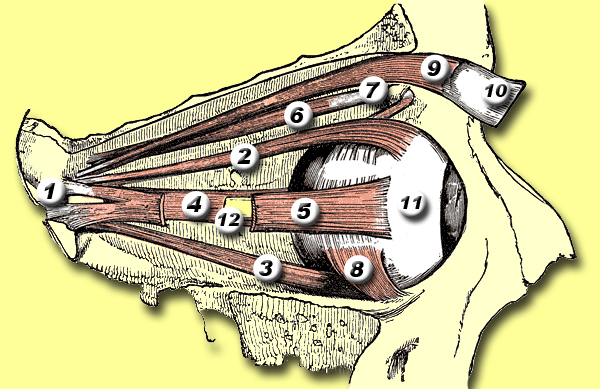
\includegraphics[width=6cm]{figures/ch2_1_oeil}
\end{center}
\caption{ Disposition des muscles oculomoteurs de l'oeil droit: 1=Tendon de Zinn, 2= Muscle droit supérieur, 3=Muscle droit inférieur, 4=Muscle droit médian, 5=Muscle droit latéral, 6=Muscle oclique supérieur, 7=Muscle oblique inférieur, 9=Élévateur de la paupière, 10=Paupière, 11=Globe oculaire, 12=Nerf optique.[Wikipedia]}
\label{oeil}
\end{figure}

Plusieurs résultats sur la régulation des mouvements par le cervelet, les ganglions de la base et le système vestibulaire se sont basés sur les mouvements des yeux \cite{Purves:2005} comme modèle basique d'intégration sensori-motrice. Dans ce chapitre, nous passerons en revue les différents types de mouvements oculaires ainsi que leur intérêt et leur utilisation dans différentes tâches, en s'intéressant en particulier aux mouvements saccadiques (les saccades) visuellement guidés. Il s'agit de mouvements rapides et précis du globe oculaire qui permettent de modifier la direction du regard vers un nouveau point d'intérêt.\\

En plus des études électrophysiologiques sur les singes, l'imagerie fonctionnelle et la stimulation magnétique transcrânienne chez les humains, ont permis d'identifier plusieurs zones corticales et sous corticales qui contribuent à la programmation des saccades \cite{Pierrot:2002}. Nous donnerons une description générale des principales structures, ainsi que les hypothèses sur leurs rôles.\\

Enfin, le système saccadique représente un site d'intégration sensori-motrice. Les stimuli lumineux se projettent sur la rétine produisant des modifications physiques et chimiques dans les récepteurs rétiniens. Ces modifications des changements d'activité des neurones et les signaux représentant cette information visuelle reçue seront transmis au système nerveux central sous forme d'impulsions. Ensuite, une fois cette information traitée, une réponse motrice est ordonnée aux muscles agissant sur les globes oculaires. C'est ainsi qu'on considère que le système moteur est au service du système sensoriel par lequel il est régi. Nous examinerons les aspects d'intégration visuo-motrice dans la troisième section de ce chapitre. \\

Mais avant cela, un rapide survol de l'anatomie de l'oeil est nécessaire.\\

\section{L'anatomie oculaire : la rétine}

L'anatomie du système visuel des primates a été intensivement étudiée chez le singe macaque étant donné sa ressemblance avec celui de l'Homme (pour une revue voir \cite{Leigh:2004}). L'oeil capte les rayons lumineux, l'information est transmise aux aires visuelles via le nerf optique. La partie de l'oeil sensible à la lumière est la rétine. Il s'agit d'une mince surface d'environ $0,5 mm$ d'épaisseur située au fond de chaque oeil, couvrant $3/4$ du globe oculaire. Elle possède une structure complexe composée de couches successives de neurones (figure \ref{Ret}). La couche la plus externe est adhérente à la choroïde, qui est une couche vasculaire de couleur noire qui tapisse les trois cinquièmes postérieurs du globe oculaire. Elle absorbe les rayons lumineux inutiles pour la vision et nourrit les photo-récepteurs de la rétine grâce à sa richesse en vaisseaux sanguins. Les premiers phénomènes de la vision débutent dans la couche de photorécepteurs (cônes et bâtonnets) qui compte environ $130$ $millions$ bâtonnets sensibles à la lumière faible et assurent la vision nocturne et $65$ $millions$ de cônes qui répondent à une luminosité intense, permettent la vision des couleurs et la distinction des détails \cite{Gregory:2000, Sekuler:1990}.\\ 

\begin{figure}[h]
\begin{center}
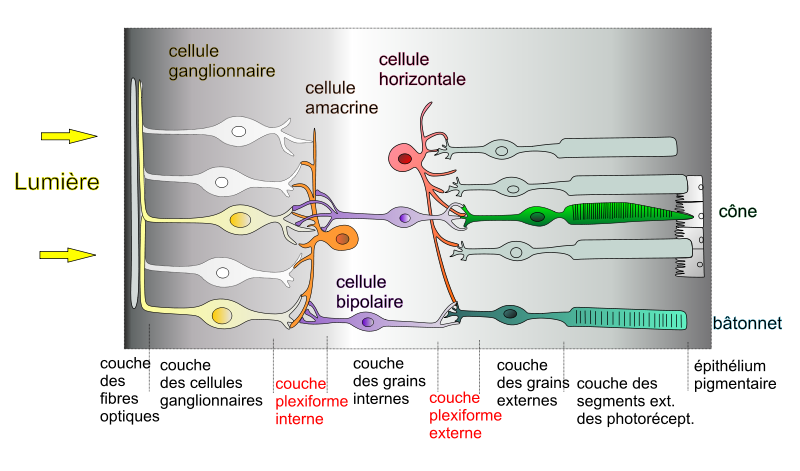
\includegraphics[width=17cm,height=10cm]{figures/ch2_2_Retina}
\end{center}
\caption{ Structure de la rétine : La couche monostratifiée des cellules photoréceptrices glutaminergiques (les cônes au sein de la fovéa, ou les bâtonnets plus en périphérie). La couche plexiforme externe formée des cellules horizontales de type H1 et H2. La couche nucléaire interne (ou couche des grains internes) formée des cellules bipolaires GABAergiques et glycinergiques, de plusieurs types (les cellules bipolaires périphériques, spécifiques des bâtonnets, et les cellules bipolaires centrales, spécifiques des cônes, lesquelles comptent au moins les sous-classes suivantes : géantes, diffuses, midget et S-cône). La couche plexiforme interne formée des cellules amacrines. La couche des cellules ganglionnaires dont les axones se connectent de façon excentrée au niveau de la macula (comprenant moins de couches et dépourvue de cellules photosensibles) pour donner le nerf optique [Wikipedia].}
\label{Ret}
\end{figure}

%%%%%%%%%%%%%%%%%%%%%%
Ensuite, le flux nerveux est transmis jusqu'aux cellules ganglionnaires qui sont les neurones de sortie de la rétine chez les vertébrés. Elles reçoivent les informations sur le monde visuel via des cellules bipolaires et des cellules amacrines (interneurones rétiniens). Mais à la différence des photorécepteurs qui répondent à la lumière par un changement du potentiel de membrane, ces cellules transmettent l'information visuelle sous forme de potentiels d'action. Elles sont activées de manière permanante même en l'absence de lumière mais leur activité tonique est modulée par les signaux d'entrée provenant des neurones rétiniens. Tout comme les neurones des différentes couches de la rétine, chaque cellule ganglionnaire couvre une région de notre champ visuel\footnote{Le champ visuel est défini par la partie de l'espace que l'oeil immobile peut voir autour du point qu'il fixe. On distingue le champ visuel monoculaire (exploré en clinique) du champ visuel binoculaire correspondant à la superposition par la partie nasale des deux champs monoculaires. Les limites périphériques d'un champ visuel normal varient selon le secteur: $90°$ à $110°$ dans le champ temporal, $60°$ à $90°$ dans le champ nasal, $60°$ dans le champ supérieur et $75°$ dans le champ inférieur. Le passage des rayons lumineux émanant d'un objet, à travers les milieux transparents de l'oeil, inverse les images des objets du champ visuel sur la surface de la rétine, dans le sens bas-haut et droite-gauche. Les objets de la partie temporale sont vus par le champ rétinien nasal et ceux de la partie supérieure du champ visuel par le champ rétinien inférieur \cite{Flament:2002}.} appelée le champ récepteur de ce neurone, c'est à dire que la présence d'un stimulus approprié dans cette région modifie l'activité nerveuse de cette cellule. Le champ récepteur des cellules ganglionnaires est très petit au centre de la rétine et devient de plus en plus grand vers la partie périphérique.\\

En effet, dans la rétine, l'acuité visuelle\footnote{Elle est définie comme la capacité à distinguer les plus fins détails spatiaux de haut contraste.} décroît du centre de la rétine (\textit{la fovéa} qui est la partie centrale de la macula\footnote{La macula est la zone de la rétine caractérisée par une concentration maximale de cônes. Située au fond de l'oeil, la macula a un diamètre d'environ $2$ $mm$. La macula contient en son centre une petite dépression appelée la fovéa : entièrement composée de cônes serrés les uns contre les autres, celle-ci est la zone d'acuité maximale de l'oeil [wikipedia]}) vers la périphérie. Cette propriété est attribuée à une variation de la densité des photo-récepteurs qui décroît du centre à la périphérie \cite{Marilly:1999}. 

\begin{figure} [htbp]
\begin{center}
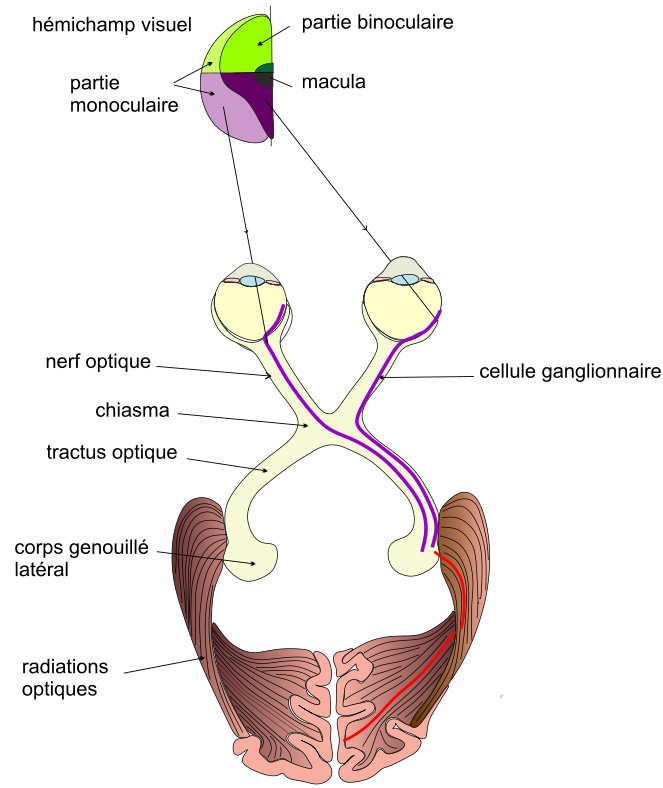
\includegraphics[width=10cm,height=12cm]{figures/ch2_3_Voies}
\end{center}
\caption{Le chiasma optique permet la \textit{décussation} d'un certain nombre d'axones en provenance de la rétine pour assurer le traitement croisé de l'information visuelle. C'est donc le lieu du rassemblement des informations visuelles d'un même hémichamp (demi-champ) visuel captées par les deux rétines. La grande majorité des fibres nerveuses du tractus optique projette sur le corps genouillé latéral dans la partie dorsale du thalamus, le relais principal de la voie qui mène au cortex visuel primaire [Wikipedia]. }
\label{Dec}
\end{figure}

La fovéa est définie donc comme la région o\`u l'acuité visuelle est maximale, ses champs récepteurs se trouvent au centre du champ visuel. On distingue donc la vision centrale (centrée sur la fovéa) qui permet une bonne qualité d'analyse de formes et de couleurs en termes de précision, de la vision périphérique plus efficace dans la détection de mouvements. Les connexions entre les différentes cellules de la rétine centrale sont unitaires (Chaque cône n'y est connecté qu'à une cellule bipolaire, elle même liée qu'à une cellule ganglionnaire). Par contre au niveau de la rétine périphérique, les connexions sont convergentes puisque la densité des cônes diminue considérablement par rapport au nombre de cellules ganglionnaires (plusieurs récepteurs sont connectés à chaque cellule ganglionnaire) et l'acuité est corrélativement fortement réduite. L'organisation des circuits nerveux rétiniens implique donc que la rétine centrale (fovéa) est plus discriminative (reconnaissance de l'information) que la rétine périphérique. Par contre cette dernière est beaucoup plus sensible (détection de l'information).\\



Enfin, les axones des cellules ganglionnaires se rassemblent pour constituer le nerf optique \cite{Purves:2004} qui projette vers les centres visuels du cerveau, principalement le corps genouillé latéral du thalamus et le colliculus supérieur (décrits dans la suite). Les nerfs optiques se réunissent pour former \textit{le chiasma optique} juste en avant de l'hypophyse. Le chiasma optique permet le changement de côté d'un certain nombre d'axones (du coté nasal) en provenance de la rétine  pour assurer le traitement croisé de l'information visuelle (fig \ref{Dec}). Ces axones vont changer de côté au niveau du chiasma optique pour faire en sorte que la moitié gauche du champ visuel soit perçue par l'hémisphère cérébral droit, et vice-versa.\\%Décussation

Les informations visuelles sont ensuite traitées corticalement. Suite aux travaux de \cite{Ungerleider:1982}, on distingue fonctionnellement deux grandes voies de traitement cortical de l'information visuelle : la voie \textit{ventrale}, celle de l'identification des objets et la voie \textit{dorsale}, celle de la localisation des objets et la préparation de l'action. Leurs descriptions seront détaillées plus loin dans le texte. Nous allons nous intéresser plus à la voie dorsale qui traite les informations liées aux mouvements des yeux et le contrôle visuel de l'action pour permettre en particulier les mouvements en direction ou non des objets présents. On commencera donc par passer en revue les différents types de mouvements oculaires puis une description fonctionnelle des différentes strutures corticales et sous-corticales impliquées dans l'encodage de ces mouvements sera donnée. 

\section{Les mouvements oculaires}

Ces mouvements de rotations que les globes oculaires effectuent autour de leurs centres modifient la direction de la ligne de regard. Ils servent à explorer les scènes visuelles, à réagir à l'apparition de nouveaux objets, à suivre des objets mobiles. Ils peuvent être volontaires (recherche d'un élément dans l'environnement) ou réflexes (compensation des mouvements de la tête). On distingue les mouvements effectués par un seul oeil, dits \textit{mouvements de duction}, des mouvements simultanés des deux yeux qui permettent une vision binoculaire. Les deux yeux peuvent bouger, soit de manière identique, on parle donc de \textit{mouvements de version} (ou mouvements conjugués), soit de manière symétrique, on parle alors de \textit{mouvements de vergence}. \\

La plus ancienne classification fonctionnelle des mouvements des yeux date de 1903 \cite{Dodge:1903}. Dodge et Cogan étaient les premiers à distinguer \textit{les saccades oculaires} des autres mouvements des yeux (poursuite lente, vergence, réflexe optocinétique, réflexe vestibulo-oculaire). Les catégories oculomotrices décrites à l'époque sont encore en usage aujourd'hui. Nous nous sommes intéressés dans nos travaux aux saccades et pour bien situer ce type de mouvements nous donnons dans la suite une revue des différents mouvements chez le primate. \\
 

\subsection{Les mouvements de stabilisation}

Il s'agit de mouvements oculaires qui agissent en synergie pour permettre une vision nette et centrale quand le corps est mobile ou quand l'objet visionné est mobile. Les trois classes de mouvements de yeux qui opèrent dans la même gamme de vitesses sont: la poursuite lente, le nystagmus optocinétique qui consiste en une alternance entre des mouvements oculaires rapides et lents provoquée par un grand champ de mouvement visuel et le réflexe vestibulo-oculaire qui stabilise le regard lors des mouvements de la tête. \\

Chez les primates ayant une région fovéale, les mouvements oculaires de poursuite lente (\textit{smooth poursuit}) permettent de suivre de près un objet en mouvement sans que l'image de l'objet ne s'écarte de la fovéa. Lorsque le mouvement de poursuite est bien développé, il s'effectue de façon continue, lente, fluide et régulière, sans changements brusques de points de fixation (voir \cite{Leigh:1999, Ilg:1997} pour un aperçu). Ils sont exécutés volontairement mais la plupart des gens sont incapables d'initier un mouvement de poursuite sans un signal visuel en mouvement. En outre, la poursuite de cibles mobiles avec des vitesses supérieures à $30°/s$ nécessite souvent des mouvements de rattrapage. \\

Ce type de mouvement n'existe que chez les primates \cite{Buttner:1988} et se distingue du réflexe opto-cinétique (\textit{optokinetic nystagmus}) commun à tous les mammifères. Le réflexe opto-cinétique réagit aux mouvements d'ensemble du champ visuel, alors que la poursuite opère sur une petite région. Ce reflexe consiste en deux phases. D'abord, une phase lente avec de lisses mouvements oculaires de compensation dans la direction du mouvement. Ensuite, une phase rapide avec des mouvements dans la direction opposée à la phase lente pour repositionner les yeux dans les plus brefs délais comme dans le cas de suivi des arbres à travers les fenêtres d'un train en mouvement. Il permet donc de réajuster le regard suite à une rotation prolongée et dirige le regard vers la cible à venir.\\

Il se distingue aussi du réflexe vestibulo-oculaire qui est indépendant de la stimulation visuelle et est provoqué par des mouvements de tête, même dans l'obscurité. Il permet de stabiliser la position des yeux par rapport au monde extérieur et compense donc les mouvements de la tête pour maintenir l'image de l'environnement stable sur la rétine pendant les rotations brèves de la tête. Une vision claire lors de la marche, par exemple, n'est possible que parce que le réflexe vestibulo-oculaire est assez rapide pour générer des mouvements oculaires compensatoires\cite{Grossman:1988}. \\

Avec ces mouvements, les primates peuvent suivre activement des objets en mouvements avec leurs yeux et peuvent aussi garder les yeux sur des objets fixes lorsque la tête ou le corps entier bouge. Ces mouvements oculaires lents coexistent et sont souvent utilisés en conjonction pour stabiliser le regard et interagir avec les objets dans un environnement dynamique \cite{Leigh:1987,Paige:1983,Yee:1983}.\\

\subsection{Les mouvements de vergence}

La vergence est le mouvement simultané des deux yeux dans des directions opposées tout en maintenant une vision binoculaire \cite{Cassin:1990}. Les deux yeux convergent pour voir une cible plus proche et divergent pour fixer une cible plus éloignée. Le système de vergence se développe pendant les trois premiers mois du nourrisson et se dégrade à partir de la cinquantaine. \\

Les mouvements de vergence sont principalement provoqués par une disparité entre les images des deux yeux. La disparité vient du fait qu'une image se projette sur des emplacements différents sur les deux rétines. Ceci provoque une diplopie, c'est à dire la perception d'une image double. La fusion des images rétiniennes des deux yeux est possible même si les images ne sont pas exactement confondues. On appelle aire de Panum l'aire dans laquelle deux images rétiniennes fusionnent pour donner une unique perception. La taille de cette aire dépend des personnes et de l'excentricité de la cible. Elle est de l'ordre d'une dizaine de minutes d'arc au niveau de la fovéa et peut aller jusqu'à $40$ $minutes$ $d'arc$ en excentricité.\\


Les mouvements de vergence sont de petite amplitude, de l'ordre de quelques degrés, environ $3°$ par oeil. Les temps de réaction sont de $160$ $ms$ à $200$ $ms$ et la vitesse de l'ordre de $25\degres/s$. Outre les mouvements de convergence ou divergence, il existe aussi une activité de vergence tonique qui maintient les yeux au repos avec un certain angle de vergence. Cette vergence de repos dépend de l'orientation des yeux dans les globes. \\

\subsection{Les mouvements saccadiques}

Les saccades oculaires sont des mouvements rapides et précis du globe oculaire permettant de modifier la direction du regard vers un nouveau point d'intérêt (de fixation). Ces mouvements brusques placent l'image du point de fixation de la scène visuelle sur la \textit{fovéa} ($1.5 mm$ de diamètre), assurant ainsi une intégration et une analyse plus fine de l'information visuelle (processus de fovéation).\\

La durée des saccades varie entre $20$ et $200$ $ms$. Cette durée dépend en particulier de l'\textit{amplitude du mouvement saccadique}: la distance angulaire que l'oeil doit survoler pendant le mouvement. Les relations stéréotypées entre la durée et l'amplitude d'une saccade, d'une part, et entre la vélocité maximale d'une saccade et son amplitude, d'autre part, sont connues sous le terme de séquence principale de la saccade (\textit{saccadic main sequence} \cite{Bahill:1975}). Pour des amplitudes comprises entre 4° et 40°, la durée d'une saccade dépend presque linéairement de son amplitude et la vélocité maximale dépend logarithmiquement ou exponontiellement de l'amplitude \cite{Becker:1991,Garbutt:2001}.\\ %Cette amplitude va des déplacements de petite taille (lors de la lecture par exemple) jusqu'aux 4 coins d'une pièce. vitesse angulaire maximale 1000°/s
 
Les mouvements saccadiques forment une hiérarchie en partant des saccades les plus élémentaires (saccades réflexes) en réponse à des apparitions soudaines d'objets dans le champ visuel pour arriver au niveau supérieur (saccades vers des positions mémorisées après disparition de stimuli) \cite{Leigh:1999}. On peut les classer selon leur objectif comme suit :\\
\begin{itemize}

\item[$\bullet$]{\em les saccades volontaires} sont des saccades sélectionnées dans le cadre d'un comportement intentionnel. Elles sont réalisées suite à une consigne ou une décision prise en interne de déplacement du regard vers un objet (ou une cible) déjà présent dans l'environnement visuel de la personne.\\

\item[$\bullet$]{\em les saccades réflexes} se déclenchent de manière exogène par l'apparition d'un stimulus périphérique, ou par la disparition d'un stimulus de fixation. Dans les conditions naturelles, nous faisons plusieurs saccades spontanées par seconde. Elles peuvent être déclenchées par un stimulus visuel, auditif ou somesthésique.\\

\item[$\bullet$]{\em les saccades prédictives ou anticipées} servent à anticiper la recherche d'une cible, un objet ayant un mouvement régulier. Elles sont réalisées en anticipation de l'apparition d'un objet ou d'une cible.\\


\item[$\bullet$]{\em les saccades guidées par mémorisation} sont des saccades vers une position mémorisée d'un stimulus présenté dans le passé. Il s'est avéré utile d'étudier la précision de ces saccades, en particulier chez les patients présentant des lésions affectant les lobes frontaux et les noyaux gris centraux qui pourraient nuire à la mémoire de travail. Lorsque les sujets normaux tentent de faire des saccades à l'emplacement d'une cible mémorisée qu'ils fixaient quelques secondes avant, ils le font avec un peu moins de précision que si la cible était visible.\\

\item[$\bullet$]{\em les antisaccades} sont des saccades qui éloignent les yeux du stimulus visuel. Une antisaccade réussie nécessite l'inhibition d'une saccade réflexe vers l'endroit du stimulus, et le déplacement volontaire de l'oeil dans la direction opposée. En plus de regarder vers de nouvelles cibles visuelles, une partie importante du comportement saccadique est de supprimer les mouvements oculaires qui seraient apportées vers les nouveaux stimuli qui ne sont pas importants (perturbateurs). Pour étudier un tel contrôle des saccades volontaires par rapport aux réflexes, un paradigme de test spécial est appelé la tâche antisaccade. 
Dans cette tâche, il est nécessaire de supprimer une saccade vers un stimulus qui apparaît dans la périphérie de la vision pour générer une saccade volontaire de taille égale vers le côté opposé \cite{Fischer:1997}. La mesure la plus simple de la réponse à ce test concerne la direction de la saccade initiale \cite{Currie:1991}. Les sujets normaux font d'abord beaucoup d'erreurs sur cette tâche, mais après une brève période de pratique, le taux d'erreur baisse à moins de 15\%.\\

\item[$\bullet$]{\em les saccades spontanées} sont des saccades aléatoires involontaires qui peuvent être réalisées même dans l'obscurité.\\

\item[$\bullet$]{\em les micro-saccades} sont des mouvements minuscules, environ $20$ secondes d'arc et sont complètement imperceptibles en temps normal. En effet, même lors de la fixation d'un objet, l'oeil humain est dans un état constant de vibration, oscillant dans plusieurs sens à un taux d'environ $60$ vibrations par seconde. Ces micro saccades servent à rafraîchir l'image  projetée sur les cellules bâtonnets et les cellules cônes à l'arrière de l'oeil. Sans micro-saccades, regarder fixement quelque chose causerait la cessation de la vision après quelques secondes puisque les bâtonnets et les cônes répondent seulement à un changement de luminosité \cite{Pettigrew:1990}.\\

\end{itemize}
%(figure Metriques d'une saccade oculaire d'après fuchs 1967).

Il est également utile de classer les saccades selon la \textit{latence} (le temps entre l'apparition du stimulus visuel et le déclenchement du mouvement). Dans ce cas, la catégorisation est binaire: une saccade donnée est une saccade ``express'' ou elle ne l'est pas. Le temps de latence de référence est d'environ $~100 ms$. S'il est dépassé, il ne s'agit pas de saccades express. Ces saccades express sont générées par un mécanisme neuronal qui contourne les longs circuits et active les muscles de l'oeil plus directement \cite{Fischer:1983}. Il s'agit du chemin sous-cortical qui part de la rétine vers la formation réticulée en passant par le colliculus supérieur.\\

Il en résulte donc que les saccades sont caractérisées principalement par les grandeurs suivantes : la direction, l'amplitude, la vitesse et la latence. Nous aborderons dans la section suivante la description des structures corticales et sous-corticales qui participent en particulier à la génération des saccades, et plus généralement à l'intégration visuo-motrice.

\section{Les structures corticales et sous corticales impliquées dans la gestion des saccades}


Reprenons l'exemple de la conduite d'une voiture. Après avoir reçu l'information visuelle (un panneau de signalisation lumineux, feux, clignotant...) dans le lobe occipital (le cortex visuel) du cerveau du conducteur, l'intégration visuo-spatiale est assurée dans le lobe pariétal plus particulièrement dans le cortex pariétal postérieur (position relative, vitesse, ...). Une saccade peut être déclenchée soit par réflexe (suite à un signal lumineux brusque), principalement par le biais du champ oculaire pariétal, ou intentionnellement (pour lire un panneau par exemple) impliquant les champs oculaires frontaux, une zone qui semble également être impliquée dans la fixation visuelle active (les micro-saccades).\\

Si une saccade réflexe doit être inhibée (faire une saccade vers le rétroviseur à gauche et non pas vers une signalisation à droite), on passe donc au lobe frontal, le cortex préfrontal dorsolatéral semble y participer. Cette zone est également impliquée dans la mémoire spatiale à court terme et la prédiction, donc elle est fortement stimulée lors d'une tâche de navigation. Elle assure un rôle important dans les processus décisionnels de contrôle du comportement oculomoteur. En outre, les champs oculaires frontaux pourraient être stimulés puisqu'ils sont impliqués dans les contrôles de haut niveau tels que les transformations spatiales, les mouvements appris et l'ajustement des programmes moteurs. Ces régions corticales interagissent ensuite avec d'autres structures sous-corticales pour préparer l'exécution des mouvements.\\

En particulier, le colliculus supérieur code l'amplitude et la direction des saccades volontaires en se basant sur la position du stimulus (visuel: panneau ou auditif: klaxon). L'activation de cette structure est modulée par l'action d'un ensemble de noyaux sous-corticaux appelés les ganglions de la base impliqués dans la sélection de l'action. Cette structure est fortement sollicitée lors de la phase de l'apprentissage (ce qu'il faut regarder en premier avant de s'arrêter ou avant de s'insérer dans une voie rapide...). Les décisions motrices sont ensuite envoyées à la formation réticulée qui contient les centres vertical et horizontal du regard. Cette structure envoie les commandes de déclenchement de saccades vers les neurones moteurs qui innervent les muscles extra-oculaires. Ces ordres moteurs sont régulés par le cervelet qui semble être impliqué dans la correction et la coordination des mouvements (mouvements des yeux et de la tête pour la vision, des mains et des pieds pour le contrôle physique de la voiture ...).\\

Enfin, les connexions entre ces différentes structures corticales et sous-corticales sont en partie assurées par le thalamus qui permet principalement de centraliser l'information sensorielle et motrice. Nous donnerons d'abord dans cette section des descriptions plus ou moins détaillées des différentes structures impliquées dans la gestion des saccades et qui ont été introduites brièvement dans cet exemple (voir fig \ref{struct} pour une illustration). Ensuite, nous nous concentrerons dans la section suivante sur les aspects principaux de la transformation visuo-motrice.
%%%%%%%%%%%%%%%%%%%%%%%%%%%%%%%%%%%%%%%%%%%%%%%%%%%%%%%%%%%%%%%%%%%%%%%%%%%%%%%%%%%%%%%%%%%%%%%%%%%%%%%%%%%%%%%%%%%%%%%%%%%%%%%%%%%%%%%%%%%%%%%%%%%%%%%%%%%%%%%%%%%%%%%%%%%%%%%%%%%%%%%%%%%%%%%%%%%%%
%%%%%%%%%%%%%%%%%%%%%%%%%%%%%%%%%%%%%%%%%%%%%%%%%%%%%%%%%%%%%%%%%%%%%%%%%%%%%%%%%%%%%%%%%%%%%%%%%%%%%%%%%%%%%%%%%%%%%%%%%%%%%%%%%%%%%%%%%%%%%%%%%%%%%%%%%%%%%%%%%%%%%%%%%%%%%%%%%%%%%%%%%%%%%%%%%%%%%

\subsection{Le lobe occipital}

L'image du stimulus visuel capté par l'oeil est transmise au cerveau par le nerf optique. Celui-ci se termine sur les cellules du corps genouillé (géniculé) latéral [\gls{lgn}], premier relais des voies visuelles corticales. Les cellules du \gls{lgn} vont rejoindre principalement le cortex visuel primaire [\gls{v1}], appelé aussi cortex strié (les autres aires visuelles sont dites extrastriées), qui se situe dans la partie la plus postérieure du lobe occipital du cerveau et correspond à l'aire 17 de Brodmann\footnote{L'organisation cellulaire corticale est différente dans plusieurs régions du néocortex. L'anatomiste allemand Korbinian Brodmann s'est servi de ce critère pour délimiter des aires corticales distinctes fonctionnellement au début du vingtième siècle en établissant une carte cérébrale basée sur les différences d'architecture cellulaire des différentes régions du cortex.} (fig \ref{struct}). Comme pour les autres sens, la moitié droite du champ visuel est analysée par l'hémisphère gauche et inversement.\\

Le stimulus visuel est représenté sur \gls{v1} par une distribution d'activités le long d'une carte spatiale. Les différentes positions dans la carte correspondent à différentes positions dans la rétine. Cette cartographie rétinotopique est une transformation de l'image visuelle de la rétine vers \gls{v1}. La correspondance entre un endroit donné dans le champ visuel et sa projection sur \gls{v1} est très précise (même les angles morts sont représentés dans \gls{v1}). Chez l'homme et les animaux avec une fovéa, une grande partie de \gls{v1} est associée à la partie centrale du champ visuel, un phénomène connu sous le nom de ``magnification corticale''\footnote{Variation de la surface corticale dédiée à la représentation d'un stimulus en fonction de la localisation des récepteurs qu'il stimule.} \cite{Daniel:1961}.\\

\gls{v1} est hautement spécialisé dans le traitement des informations sur les objets (statiques et en mouvement), en particulier pour la reconnaissance des formes. Il semble être l'aire corticale la plus simple. Il projette principalement vers le cortex visuel secondaire [\gls{v2}] qui est formé par les aires de Brodmann 18 et 19 (fig \ref{struct}).\\

En plus des fonctions en commun avec \gls{v1}, \gls{v2} est impliqué dans des fonctions plus complexes (l'orientation des contours illusoires, la disparité binoculaires...)\cite{Qiu:2005,Ts:2009}. \gls{v2} projette sur les autres aires visuelles striées (\gls{v1}) et extrastriées (V3,V4,V5).\\

L'aire V3 se réfère à la région du cortex antérieure à \gls{v2}. Elle n'est pas très bien définie et semble posséder une sélectivité à l'orientation et au mouvement. L'aire V4 est située entre \gls{v2} et l'aire inférotemporale postérieure. Cette aire V4 est impliquée dans la perception des couleurs. Comme \gls{v1}, V4 est impliqué dans le codage de l'orientation, la fréquence spatiale et la couleur. V4 présente aussi une forte modulation attentionnelle. La plupart des études indiquent que l'attention sélective peut changer la fréquence de décharge en V4 d'un taux d'environ 20\% \cite{Moran:1985}. Des travaux récents ont montré que V4 est caractérisé par une plasticité à long terme et impliqué dans le codage de la saillance des stimuli \cite{Mazer:2003, Yang:2004}. L'aire V5, connue aussi sous le nom de l'aire temporale médiane [\gls{mt}], est située en avant du lobe occipital. Cette aire est impliquée dans la perception des mouvements et l'orientation des yeux \cite{Born:2005}.\\




L'information visuelle arrivant au niveau du cortex est donc d'abord traitée dans le lobe occipital. Ensuite, le flux nerveux suit deux voies principales, celles évoquées rapidement à la fin de la deuxième section \cite{Ungerleider:1982,Milner:1995}. La voie dorsale projette l'information visuelle dans le lobe pariétal, la voie ventrale projette l'information visuelle dans le lobe temporal (fig \ref{path}).\\

La voie ventrale (appelée aussi la voie du ``quoi ?'', \textit{the ``What'' pathway}) commence par \gls{v1}, passe par \gls{v2}, V4 puis le cortex temporal inférieur. Elle semble être impliquée dans l'identification des objets en les comparants à des représentations mémorisées. Il s'agit donc plutôt d'une voie de perception. Elle est associée à la reconnaissance des formes et la mémorisation à long terme.\\

%%%%%%%%%%
\begin{figure}
\begin{center}
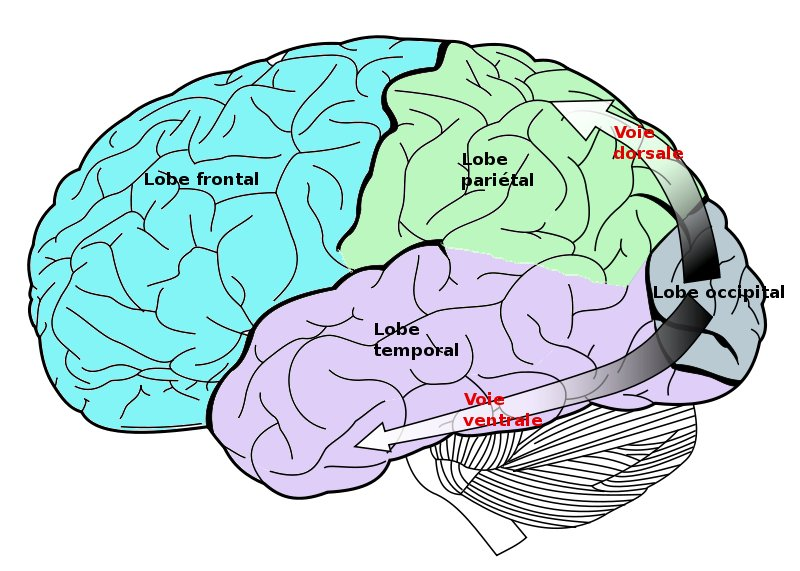
\includegraphics[width=12cm,height=8cm]{figures/ch2_4_Lobes}
\end{center}
\caption{ Les deux voies de traitement visuel. Voie ventrale : reconnaissance, identification des objets. Voie dorsale : traitement des informations, actions [Adapté de wikipedia].}
\label{path}
\end{figure}
%%%%%%%%%

La voie dorsale (appelée aussi la voie du ``comment ?'', \textit{the ``How'' pathway}) commence par \gls{v1}, passe par \gls{v2}, l'aire \gls{mt} puis le cortex pariétal postérieur [\gls{ppc}] \cite{Goodale:1992}. Elle est vouée principalement à guider spatialement les interactions avec les objets du monde visuel. Ce traitement semble être largement inconscient. La voie dorsale est considérée comme une voie d'action car en intégrant les relations spatiales avec notre environnement, ça nous permet d'interagir efficacement avec lui. Cette voie permet le contrôle des mouvements des yeux et des bras surtout quand l'information visuelle est utilisée pour guider des saccades. Nous allons nous intéresser plus à cette voie c'est pourquoi le lobe temporal ne sera pas considéré dans la suite.\\


\subsection{Le lobe pariétal}

Le lobe pariétal participe à l'intégration des informations sensorielles en provenance de différentes parties du corps, la connaissance des membres et de leurs relations, \cite{Blakemore:2005, Fogassi:2005} et  la manipulation d'objets. Certaines parties du lobe pariétal sont impliquées dans le traitement visuo-spatial, plus particulièrement le cortex pariétal postérieur (\gls{ppc}). Bien qu'il soit une zone d'intégration multisensorielle, le cortex pariétal postérieur est désigné comme la voie dorsale de la vision (par opposition à la voie ventrale dans le lobe temporal). \\

Le cortex pariétal du singe est situé en aval du gyrus post-central. Il peut être divisé en deux parties principales: une antérieure et une postérieure. La partie antérieure [\gls{apc}] contient les aires de Brodmann 1, 2, 3 et 43, et le cortex somatosensoriel primaire. La partie postérieure (\gls{ppc}) se compose de aires 5a, 5b, 7a, 7b, et les aires intrapariétales antérieures, latérales, médiales et ventrales (AIP, LIP, MIP et VIP, respectivement).\\

Chez l'homme, le \gls{ppc} peut être subdivisé en lobule pariétal supérieur (aires de Brodmann 5 et 7 correspondant aux aires 5a et 5b chez le singe) et lobule pariétal inférieur (aires de Brodmann 39 et 40 correspondant aux aires 7a et 7b chez le singe), séparés par le sillon intrapariétal [\gls{ips}], lui-même divisé en médial [\gls{mip}], latéral [\gls{lip}], ventral [\gls{vip}] et antérieur [\gls{aip}].\\

Le lobule supérieur semble avoir un rôle essentiellement somatosensoriel \cite{Rizzolatti:1997}. Par contre, le lobule inférieur semble être plus visuel; les neurones de cette région ont la particularité d'être multimodaux, c'est-à-dire qu'ils sont capables de traiter simultanément des stimuli de différentes natures (auditif, visuel, sensorimoteur, etc) \cite{DeRenzi:1982, Rizzolatti:1997}.\\

%%%%%%%%%%%%%%%%%%%%%%%%%Inferior LOBE %%%%%%%%%%%%%%%%%%%%%%%%%%%%%%%%%%%%%%%%%%%%%%%%%

%%%%%%%%%%%%%%%%%%%%%%%%%Intraparietal LOBE %%%%%%%%%%%%%%%%%%%%%%%%%%%%%%%%%%%%%%%%%%%%%%%%%

Enfin, plusieurs études menées dans les années 1990 ont montré que les différentes aires de l'\gls{ips} chez les macaques représentent les différentes parties de l'espace:
\begin{itemize}
\item L'\gls{aip} contient des neurones sensibles à la forme, la taille et l'orientation des objets à saisir \cite{Murata:2000} et à la manipulation des mains \cite{Fogassi:2005}. Il semble être impliqué dans les mouvements de saisie et le codage des objets 3D disposés avant de les saisir.
\item La \gls{mip} contient des neurones qui codent l'emplacement d'une cible en coordonnées  centrées sur le nez \cite{Pesaran:2006}.
\item La \gls{lip} contient une carte rétinotopique \cite{Kusunoki:2003} de neurones  qui représente la saillance des positions spatiales et l'attention à leur accorder. Il permet donc de guider les saccades oculaires \cite{Goldberg:2006}.
\item La \gls{vip} reçoit des projections de plusieurs modalités \cite{Avillac:2005}. Il contient des neurones avec des champs récepteurs tactiles qui codent en coordonnées centrées sur la tête et d'autres avec des champs récepteurs visuels qui codent en coordonnées centrées sur la tête ou les yeux.\\
\end{itemize}

Des études plus récentes ont montré que les humains ont les mêmes régions fonctionnelles dans le sillon intrapariétal \cite{Culham:2006}. En particulier, le champ oculaire pariétal [\gls{pef}], qui correspond à la \gls{lip} chez le singe \cite{Perry:2000}, semble aussi être organisé en coordonnées centrées sur l'oeil de sorte que son activité est mise à jour lorsque les yeux bougent \cite{Medendorp:2003}.\\

De manière plus générale, le \gls{ppc} semble être impliqué dans plusieurs tâches sensori-motrices, et plus particulièrement visuo-motrices:\\
\begin{itemize}
\item[$\bullet$] \textit{L'intégration multi-sensorielle}:
Le \gls{ppc} offre une représentation spatiale multimodale de l'information provenant de différentes modalités sensorielles (vision, audition et somatosensation) avec une copie efférente des mouvements corporels \cite{Andersen:1997}.\\
\item[$\bullet$] \textit{Le contrôle oculomoteur (initiation des saccades)}:
Après des lésions du \gls{pef} chez l'homme (mais pas après une lésion des \glspl{fef} ou des \glspl{sef}), la latence des saccades déclenchées augmente de façon significative \cite{Pierrot:1991}. Le rôle du \gls{pef} dans le processus de déclenchement de saccades (réflexes en particulier) en réponse à des stimuli visuels ou auditifs est discuté dans \cite{Leigh:2004}.\\
\item[$\bullet$] \textit{Le ``remapping'' spatial}:
Des études neurophysiologiques chez des singes montrent que le \gls{ppc} contient plusieurs représentations spatiales\footnote{Ces représentations spatiales peuvent être codées en coordonnées centrées sur le regard, sur les yeux, sur la tête ou centrées sur le corps.} de l'action et soutiennent donc son implication dans la planification des saccades \cite{Colby:1996}. Certains neurones de la \gls{lip} ont en particulier montré des changements dans l'activité neuronale pré-saccadique\footnote{ Un tel comportement n'est pas exclusif à ce champ oculaire, des activités similaires ont été observées dans les \glspl{fef} \cite{Goldberg:1990,Bruce:1985} et dans le colliculus \cite{Mays:1980}.} qui semblent être le signe d'un ``remapping'' spatial qui tient compte des mouvements de l'oeil et du corps \cite{Ross:2001,Duhamel:1992}.\\
\item[$\bullet$] \textit{L'intégration sensori-motrice}:
Il s'agit d'abord de la conversion entre les référentiels associés aux différentes parties du corps qui sont nécessaires pour l'action, car les mouvements des membres peuvent avoir besoin d'être codés dans des coordonnées spatiales différentes de celles utilisées pour la vision. L'emplacement du \gls{ppc} entre les aires visuelles primaires du cortex occipital et le cortex moteur primaire, et ses liens avec les autres aires oculomotrices telles que celles du lobe frontal, le rend idéalement placé pour servir de médiateur des transformations sensori-motrices \cite {Rizzolatti:1997, Machado:2004}. Cette fonction sera traitée avec plus de détails à la fin du chapitre.\\
\item[$\bullet$] \textit{L'attention versus l'intention }:
Plusieurs travaux ont suggéré que le \gls{ppc} est impliqué dans le codage des intentions motrices avec des régions spécialisées selon les types de mouvements \cite{Andersen:2002, Mountcastle:1975}. Contrairement à cela, Colby et Goldberg \cite{Colby:1999} ont proposé que l'activité pariétale reflète plutôt l'attention visuo-spatiale \cite{Bisley:2003}. Le lobe pariétal est supposé contenir des cartes neuronales qui représentent l'emplacement des objets saillants et les actions qui peuvent être effectuées sur eux \cite{Colby:1996}.
L'activité d'une population de neurones dans le \gls{ppc} a été évaluée par \cite{Quiroga:2006} qui ont tenté de prédire l'emplacement de la cible en se basant à la fois sur le lieu de l'attention et le type du mouvement. Comme l'a noté \cite{List:2006}, cette étude est importante pour le débat attention/intention, car si les cellules de la \gls{lip} codent seulement l'attention sur un emplacement alors le type de mouvement à faire ne devrait pas avoir d'effet sur l'activité neuronale. Les résultats suggèrent que l'activité dans le \gls{ppc} peut coder à la fois l'emplacement et l'action, ce qui rejoint la théorie prémotrice (\textit{Premotor theory}) qui porte sur la relation entre l'attention spatiale et la préparation motrice et qui propose que le mécanisme présenté habituellement comme la préparation de l'action motrice (par exemple la préparation d'une saccade oculaire) soit lui-même l'attention \cite{Rizzolatti:1994}.\\


   


\end{itemize}


%%%%%%%%%%%%%%%%%%%%%%%%%%%%%%%%%%%%%%%%%%%%%%%%%%%%%%%%%%%%%%%%%%%%%%%%%%%%%%%%%%%%%%%%%%%%%%%%%%%%%%%%%%%%%%%%%%%%%%%%%%%%%%%%%%%%%%%%%%%%%%%%%%%%%%%%%%%%%%%%%%%%%%%%%%%%%%%%%%%%%%%%%%%%%%%%%%%%%
%%%%%%%%%%%%%%%%%%%%%%%%%%%%%%%%%%%%%%%%%%%%%%%%%%%%%%%%%%%%%%%%%%%%%%%%%%%%%%%%%%%%%%%%%%%%%%%%%%%%%%%%%%%%%%%%%%%%%%%%%%%%%%%%%%%%%%%%%%%%%%%%%%%%%%%%%%%%%%%%%%%%%%%%%%%%%%%%%%%%%%%%%%%%%%%%%%%%%

\subsection{Le lobe frontal}

Le cortex frontal des primates comprend deux principales zones identifiées pour le contrôle des mouvements des yeux \cite{Schall:1997, Tehovnik:2000}: les champs oculaires frontaux [\glspl{fef}] et les champs oculaires supplémentaires [\glspl{sef}] (fig \ref{struct}).\\

\begin{figure}
\begin{center}
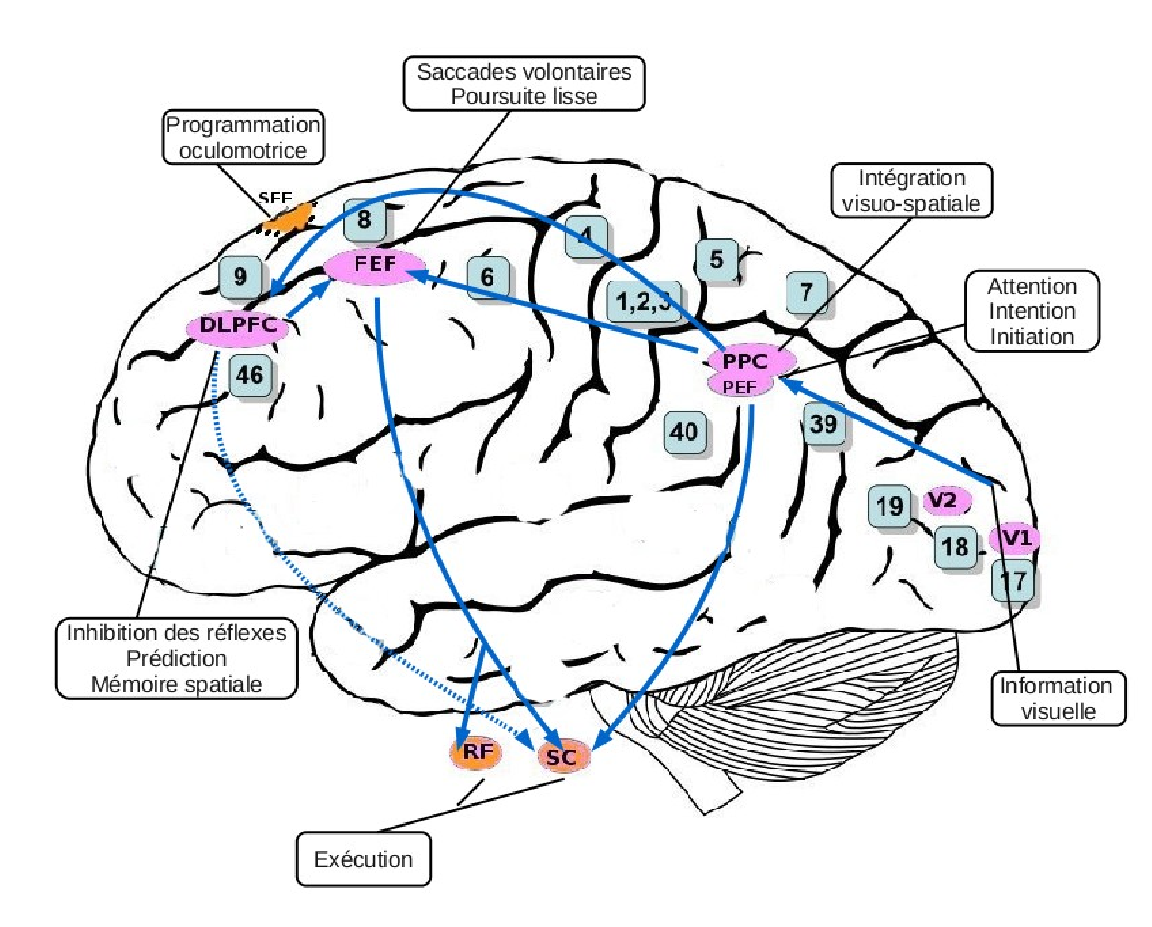
\includegraphics[width=14cm,height=10cm]{figures/ch2_5_Structures}
\end{center}
\caption{Quelques structures impliquées dans la génération des saccades. Après avoir reçu l'information visuelle dans le lobe occipital et après l'intégration visuo-spatiale dans PPC, une saccade peut être déclenchée soit par réflexe, principalement par PEF, ou intentionnellement par FEF, une zone qui semble également être impliquée dans la fixation visuelle active. Si une saccade réflexe doit être inhibée, DLPFC semble y participer. Cette zone est également impliquée dans la mémoire spatiale à court terme et la prédiction. Avec ces trois actions différentes, DLPFC assure un rôle important dans les processus décisionnels de contrôle du comportement moteur oculaire. SEF pourrait être impliqué dans les contrôles de haut niveau tels que les transformations spatiales, les mouvements appris et l'ajustement des programmes moteurs. SC code l'amplitude et la direction des saccades volontaires. FEF et SC projettent sur RF qui contient les centres vertical et horizontal du regard. RF envoie les commandes de déclenchement de saccades vers les neurones moteurs qui innervent les muscles extraoculaires. DLPFC = cortex préfrontal dorsolatéral; FEF = champ oculaire frontal; PEF = champ oculaire pariétal; PPC = cortex pariétal postérieur; RF= formation réticulée ; SC = colliculus supérieur; SEF = champ oculaire supplémentaire; Le trait discontinu correspond à l'inhibition des saccades. Les zones numérotées correspondent aux aires de Brodmann. [adapté de wikipedia]}

\label{struct}
\end{figure}
%http://brain.oxfordjournals.org/content/126/6/1460/F6.expansion
\subsubsection{Les champs oculaires frontaux}
%%%%%%%%%%%%%%%%%%%%%%%%%%%%%%%%%%%%%%%%%%%%%%%%%%%%%%%%%
Les \glspl{fef} sont situés dans le cortex préfrontal le long de la convexité latérale supérieure correspondant globalement à l'aire de Brodmann 8 et des parties des aires 9 et 6 \cite{Bruce:1985} (fig \ref{struct}). L'implication des \glspl{fef} dans le contrôle oculomoteur a été montrée par la stimulation de Ferrier de l'aire corticale 8 prémotrice chez les singes qui a provoqué des mouvements oculaires contralatéraux \cite{Ferrier:1874}. En effet, les \glspl{fef} forment une structure topographique et représentent les cibles des saccades dans des coordonnées rétinotopiques \cite{Bruce:1985}. Leur stimulation chez le singe rhésus suscite des mouvements des yeux vers une direction spécifique ainsi que la dilatation pupillaire. Chez l'homme l'activation des \glspl{fef} pendant les saccades a été démontrée par les travaux de \cite{Melamed:1979, Petit:1993}.\\

Les cellules des \glspl{fef} s'activent en réponse sélective à des stimuli visuels fixes ou mobiles à portée des bras, ainsi qu'à des stimuli tactiles et auditifs \cite{Rizzolatti:1981}. Ces cellules sont fortement impliquées dans la médiation de l'attention visuelle et la coordination des réactions de la tête, des bras et des yeux \cite{Denny:1966, Gottlieb:1994, Macavoy:1991, Pragay:1987, Segraves:1987, Wagman:1961}. Les \glspl{fef} permettent en particulier de guider le regard dans le choix des cibles en transformant l'information visuelle en une réponse d'orientation \cite {Schall:2002, Schall:2004, Wurtz:1980, Segraves:1987} (certaines cellules signalent l'emplacement des stimuli bien visibles et significatifs qui peuvent être des cibles pour les saccades volontaires) et de contrôler si et quand une saccade vers une cible donnée est déclenchée. Des lésions des \glspl{fef} peuvent donc altérer la capacité de réaliser des saccades volontaires ou augmenter leurs latences \cite{Stuphorn:2002, Macavoy:1991, Schall:2002}.\\

Les \glspl{fef} sont aussi impliqués dans des mouvements de poursuite lente \cite{Gottlieb:1994} et le guidage des mouvements lors de la lecture et l'écriture \cite{Ritaccio:1992}. Enfin, l'activité des neurones dans les \glspl{fef} met en évidence un rôle d'anticipation \cite{Gottlieb:1994, Pragay:1987}. En fait, certains neurones s'activent avant qu'une réponse des yeux ne soit déclenchée et continuent à tirer à une cadence élevée jusqu'à ce que le comportement soit lancé. \\




%%http://brainmind.com/FrontalEyeFieldsArea8.html

\subsubsection{Les champs oculaires supplémentaires}

La région des \glspl{sef} a d'abord été décrite chez les primates non humains. Elle occupe la partie la plus rostrale du cortex prémoteur dorsal appelée l'aire F7 \cite{Matelli:1991}. Elle projette vers des structures corticales et sous-corticales incluses dans la génération de saccades \cite{Huerta:1990, Parthasarathy:1992, Schall:1993, Shook:1990}. Ces connexions sont plus diffuses que celles des \glspl{fef}. L'organisation fonctionnelle des \glspl{sef} a été étudiée par l'analyse de l'activité pré-saccadique et la stimulation électrique. Ils ont été d'abord caractérisés par John Schlag et ses collègues comme une zone où la stimulation électrique de faible intensité peut évoquer des saccades \cite{Schlag:1987}. Puis il a été montré que la stimulation des \glspl{sef} produit des mouvements coordonnés des yeux et de la tête \cite{Martinez:2003} d'o\`u l'hypothèse que les \glspl{sef} encodent les mouvements saccadiques centrés sur la tête et non pas sur l'oeil (en coordonnés rétiniennes).\\

En effet, les neurones dans les \glspl{sef} réagissent à des stimuli visuels et acoustiques et sont actifs avant et pendant les mouvements oculaires \cite{Berdyyeva:2009, Bon:1991, Ohmae:2008, Schlag:1992,Nakamura:2005, Uchida:2007} participant en particulier à la planification, l'exécution et le contrôle  des saccades volontaires, réflexes et les mouvements de poursuite lente.\\ 

%, Hanes et al 1995;. Heinen, 1995; Lee et Tehovnik 1995; Moorman et Olson, 2007a, b; Nakamura et al 2005;. Ohmae et al 2008;. Pouget et al 2005, S
Les similitudes anatomiques et physiologiques entre les \glspl{sef} et les \glspl{fef} ont conduit à l'hypothèse qu'ils agissent en parallèle \cite{Amador:2004, Russo:2000, Tehovnik:2000}. Cependant, de nombreuses caractéristiques les distinguent. Les saccades évoquées par la microstimulation des \glspl{fef} sont généralement vectorielles: les yeux se déplacent de la même distance dans le même sens quelle que soit la position initiale. En revanche, celles évoquées par la microstimulation des \glspl{sef} ont tendance à être orientées but (convergentes): en partant de différentes positions initiales, les yeux arrivent à une seule position finale \cite{Martinez:2004, Park:2006}.\\
%, Russo et Bruce 1993; Schall 1991; Schlag et Schlag-Rey, 1987; Tehovnik et Lee, 1993

Les \glspl{sef} présentent en plus des profils d'activité neuronale pré-saccadique nettement différents de ceux enregistrés dans les \glspl{fef} et qui semblent en plus dépendre du contexte \cite{Amador:2004, Chen:1995, Isoda:2002,  Ohmae:2008, Uchida:2007}.
%Coe et al 2002, 2003; Lu et al . 2002;. Mushiake et al 1996; Nakamura et al 2005,Olson et Gettner 1995, 1999; Schlag-Rey et al 1997;. Tremblay et al 2002, 
L'activation neuronale dans les \glspl{sef} est en particulier corrélée avec le temps de déclenchement de la saccade et permet une prédiction partielle de l'erreur et la probabilité d'annulation \cite{Nakamura:2005, Amador:2000, Roesch:2003, Stuphorn:2000}.\\

Il en résulte que le rôle des \glspl{sef} dans le contrôle du comportement oculomoteur ne se réduit pas à l'initiation de saccades. Cette région s'avère être impliquée dans des aspects de haut niveau de contrôle de mouvements oculaires comme les transformations spatiales complexes \cite{Olson:1995}, les mouvements appris\cite{Chen:1995}, les fonctions cognitives exécutives \cite{Stuphorn:2006} et contribue à l'ajustement dynamique de la génération de saccades \cite{Stuphorn:2010}.\\

\subsubsection{Le cortex pr\'efrontal dorsolat\'eral}
%%%http://brain.oxfordjournals.org/content/127/3/460.full
Une autre région située sur la surface dorsolatérale du lobe frontal, participe au contrôle des saccades volontaires: le cortex préfrontal dorsolatéral [\gls{dlpfc}]. Elle correspond aux aires de Brodmann 46 et 9 situées dans le gyrus frontal moyen et le cortex adjacent (fig \ref{struct}). Le \gls{dlpfc} diffère des autres champs oculomoteurs par le fait que sa stimulation ne déclenche pas de saccades.\\

Les patients atteints de lésions du \gls{dlpfc} ont des difficultés à inhiber les saccades réflexes. Dans la tâche anti-saccade, ces lésions provoquent une augmentation du pourcentage d'erreurs due à l'affaiblissement des facultés d'inhibition de mouvements oculaires réflexes \cite{Pierrot:2003}. En revanche, les patients atteints de lésions des \glspl{fef} ont un pourcentage normal d'erreurs sur la même tâche mais leurs anti-saccades correctes s'effectuent avec un temps de latence plus long que chez les sujets normaux. Ainsi, il a été supposé qu'au cours de la tâche anti-saccade, l'inhibition de saccades réflexes mal acheminées est due au \gls{dlpfc}, alors que le déclenchement intentionnel des antisaccades correctes dépend des \glspl{fef} \cite{Rivaud:1994, Pierrot:2003}.\\

Le \gls{dlpfc} est supposé aussi être impliqué dans la mémorisation à court terme (jusqu'à 20 secondes) de l'information visuo-spatiale importante (position d'une cible par exemple). En effet, l'activité des neurones du \gls{dlpfc} chez le singe, lors des tests de saccades guidées par des cibles mémorisées, montre la présence d'une carte mémoire topographique \cite{Sawaguchi:2001}. Chez l'homme, on remarque aussi une activation du \gls{dlpfc} lors de l'exécution de la même tâche \cite{Sweeney:1996}. De plus, lorsque le \gls{dlpfc} chez le singe est inactivé pharmacologiquement, les saccades guidées par la mémoire sont altérées et le pourcentage d'erreurs augmente \cite{Sawaguchi:1994}, de même pour les sujets humains qui sont atteints de lésions du \gls{dlpfc} \cite{Pierrot:2003} .\\

Enfin dans ces derniers cas, les saccades prédictives sont également altérées. Le \gls{dlpfc} semble également être la structure la plus impliquée quand une réponse est prédite à un emplacement spécifique (avant l'apparition du stimulus). Vraisemblablement, la mémoire de travail est nécessaire pour générer des réponses prédictives \cite{Pierrot:2003}.\\

Ces résultats suggèrent que le \gls{dlpfc} joue un rôle crucial dans les processus décisionnels, la préparation de saccades en inhibant les saccades réflexes indésirables (processus d'inhibition intentionnelle), le maintien  de l'information en mémoire pour des saccades volontaires (processus de mémorisation spatiale à court terme) et la facilitation des saccades anticipatrices (processus de prédiction), en fonction des circonstances environnementales.\cite{Pierrot:2003, Leigh:2006}.\\



%%%%%%%%%%%%%%%%%%%%%%%%%%%%%%%%%%%%%%%%%%%%%%%%%%%%%%%%%%%%%%%%%%%%%%%%%%%%%%%%%%%%%%%%%%%%%%%%%%%%%%%%%%%%%%%%%%%%%%%%%%%%%%%%%%%%%%%%%%%%%%%%%%%%%%%%%%%%%%%%%%%%%%%%%%%%%%%%%%%%%%%%%%%%%%%%%%%%%
%%%%%%%%%%%%%%%%%%%%%%%%%%%%%%%%%%%%%%%%%%%%%%%%%%%%%%%%%%%%%%%%%%%%%%%%%%%%%%%%%%%%%%%%%%%%%%%%%%%%%%%%%%%%%%%%%%%%%%%%%%%%%%%%%%%%%%%%%%%%%%%%%%%%%%%%%%%%%%%%%%%%%%%%%%%%%%%%%%%%%%%%%%%%%%%%%%%%%





\subsection{Le colliculus supérieur}




Le colliculus supérieur [\gls{sc}] est une structure sous corticale qui se trouve sur le tectum du mésencéphale. Cette structure est directement impliquée dans le mécanisme de génération et de contrôle des saccades \cite{Nolte:1993,Ziad:1999}. Il existe deux colliculi supérieurs, un dans chaque hémisphère du cerveau (symétrie bilatérale du cerveau).\\


Le \gls{sc} sert de site d'intégration sensori-motrice qui reçoit des entrées somato-sensorielles, auditives et visuelles \cite {Nolte:1993}. Ses entrées visuelles proviennent soit directement de la rétine ou soint indirectement en passant par le cortex (modulé par l'intervention d'autres structures). L'intégration permet de transformer les entrées sensorielles portant sur la position du stimulus pour fournir les ordres ou les prédictions de déplacements à des muscles extra-oculaires par l'intermédiaire des neurones moteurs \cite {Wurtz:1996, Nolte:1993}.\\

Une caractéristique clé du \gls{sc} est son organisation en couches. La couche superficielle est une couche visuelle qui reçoit des informations directement des cellules ganglionnaires de la rétine. Chaque site de cette couche est activé par un stimulus optimal présent dans une position particulière dans le champ visuel. Cependant, la couche profonde constitue une carte motrice organisée topographiquement: les vecteurs saccades résultant d'un stimulus visuel dépendent de la position du stimulus.\\


De nombreux modèles ont étudié le rôle du \gls{sc} (cf. \cite {Girard:2005} pour une revue). \cite{Findlay:1999} soulignent que sa principale fonction est de décider quand et où la saccade doit être effectuée. Plus tard, \cite {Godijn:2002} ont proposé un modèle d'intégration compétitive fondé sur de solides preuves expérimentales au niveau comportemental, qui indique que toutes les informations (exogènes versus endogènes, spatiales versus traitement temporel) peuvent être intégrées dans une seule carte motrice considérée comme un modèle du \gls{sc}. Plus de données sur cette structure et sur son implication dans la génération des saccades seront détaillées dans le chapitre 3 qui portera sur la proposition d'un modèle du \gls{sc}.\\

\subsection{Les ganglions de la base}

Les noyaux gris centraux (appelés encore les ganglions de la base) [\gls{bg}] sont un ensemble de noyaux situés des deux côtés du thalamus, en dehors et au-dessus du système limbique. Plusieurs études suggèrent que les \gls{bg} participent à la régulation de l'activité corticale par un mécanisme de désinhibition (retrait de l'inhibition) de l'activité thalamique considéré comme struture de centralisation des informations sensorielles et motrices. Ces noyaux assurent un ensemble d'intégration dans des circuits distincts fonctionnellement. En particuler, ces noyaux participent à la modulation de l'activité colliculaire via le circuit oculomoteur. \\

De manière schématique, les \gls{bg} agissent de deux manières sur les mouvements oculaires. D'abord, ils facilitent l'initiation des saccades volontaires générées dans un contexte de comportements appris, de prédiction ou de récompense retardée. Cette facilitation est réalisée par la désinhibition des couches intermédiaires du \gls{sc} qui sont sous inhibition tonique (empêchant le déclenchement de saccades). Le colliculus supérieur est alors ``libéré'' et la génération de saccades est rendue possible. Ensuite, ils permettent d'empêcher la génération de saccades réflexes non souhaitées \cite{Leigh:2006}. Une description plus détaillée de cette structure sera donnée dans le chapitre 4 en abordant, en particulier, son rôle dans la sélection de l'action.\\

\subsection{La formation réticulée}


La formation réticulée [\gls{rf}] est une structure nerveuse du tronc cérébral. De manière générale, elle permet la coordination et la synthèse des actions. Le système réticulé intervient dans la régulation de grandes fonctions vitales telle que la respiration et les cycles éveil-sommeil, la motricité en général et dans des fonctions cognitives telles que l'attention. Elle reçoit des entrées de pratiquement tout le cerveau. La \gls{rf} est en particulier chargée de générer les saccades oculaires permettant d'amener le centre d'intérêt sur la fovéa.\\

La direction des mouvements oculaires est pilotée par deux centres de la \gls{rf} (deux générateurs saccadiques):
\begin{itemize}
\item les mouvements horizontaux par la formation réticulée pontique paramédiane [\gls{pprf}] qui se trouve dans la région caudale du tronc cérébral, le long de la ligne médiane (centre horizontal du regard).
\item les mouvements verticaux par la formation réticulée mésencéphalique [\gls{mrf}] (centre vertical du regard). 
\item les mouvements obliques proviennent de leur action conjointe.\\
 \end{itemize}

\begin{figure}
\begin{center}
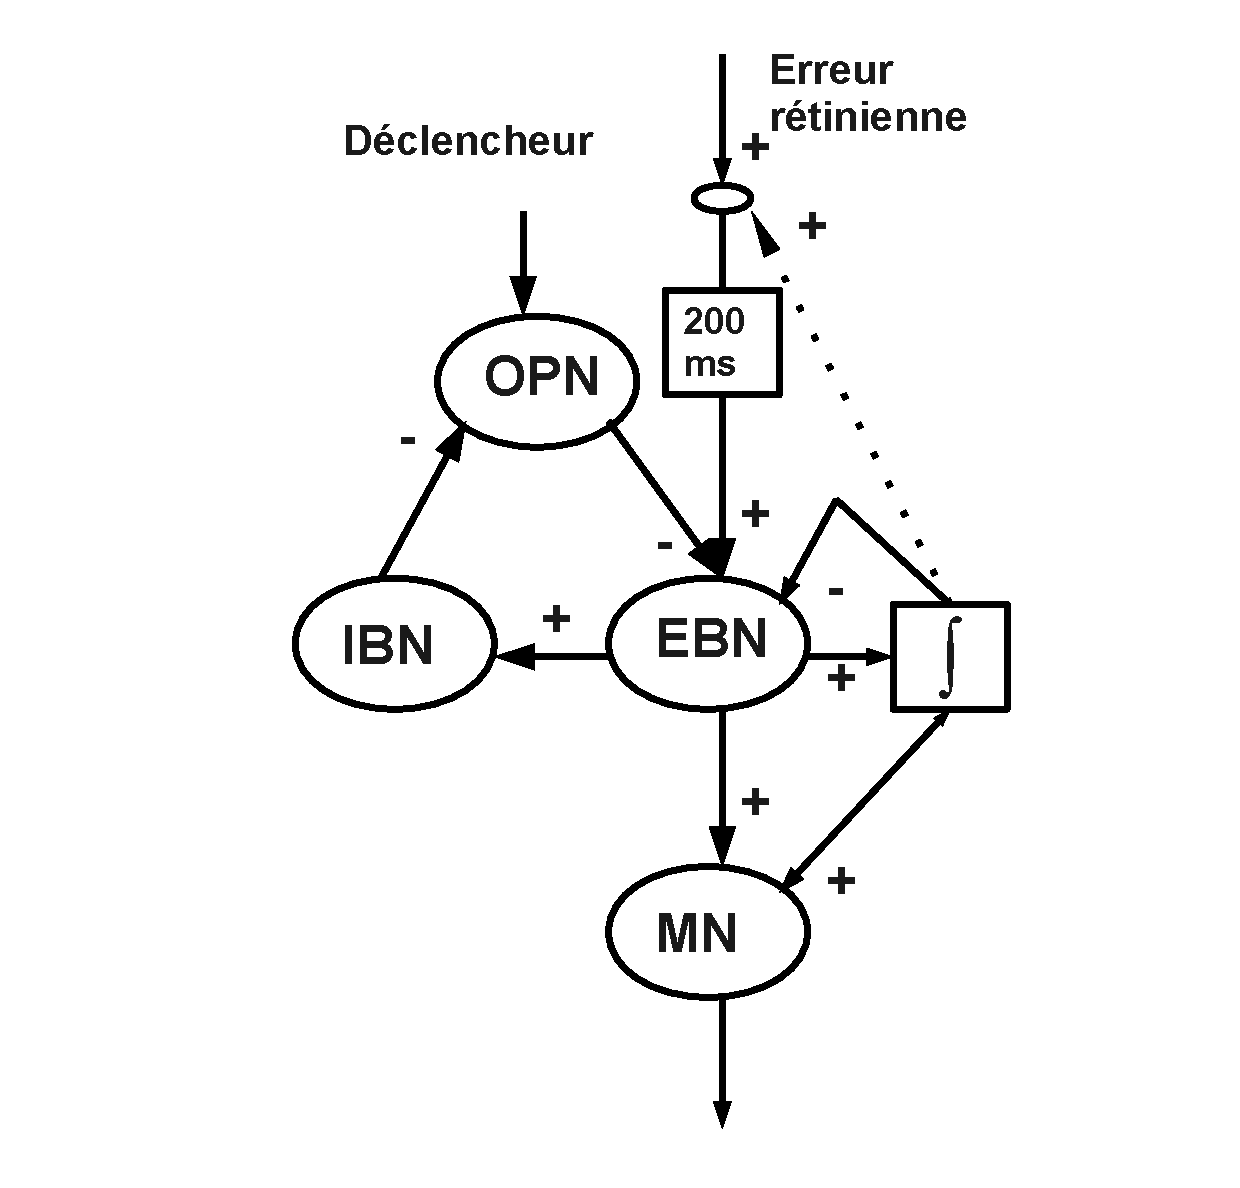
\includegraphics[width=0.5\textwidth]{figures/ch2_6_Robinson}
\end{center}
\caption{Le modèle original du générateur saccadique proposé par \cite{Robinson:1975} avec un seul intégrateur et un feedback local. Les (+) désignent les projections excitatrices et les (-) désignent les projections inhibtrices}
\label{robinson}
\end{figure}

Plusieurs types de neurones de la \gls{rf} assurent une fonction prémotrice de générateurs saccadiques \cite{Scudder:2002} en projettant vers les motoneurones [\gls{mn}] du tronc cérébral commandant les muscles oculaires. L'activité tonique des \gls{mn} est assuré par des neurones toniques [\gls{tn}]. Les \gls{tn} et les \gls{mn} qui innervent directement le muscle droit externe ipsilatéral reçoivent des projections des neurones phasiques excitateurs [\gls{ebn}] pendant les saccades ipsilatérales. Des neurones phasiques inhibiteurs [\gls{ibn}] s'activent, eux aussi, pendant les saccades ipsilatérales et projettent vers les \gls{mn} contralatéraux et les \gls{tn}. Par contre, des neurones omnipauseurs [\gls{opn}] s'activent pendant les phases de fixation et sont inactifs pendant les saccades. Ils inhibent les neurones phasiques à latence moyenne [\gls{mlbn}] qui s'activent avant le déclenchement d'une saccade. Enfin, des neurones phasiques à longue latence [\gls{llbn}] déchargent à leur fréquence maximale au moment de déclenchement de la saccade. Les interactions entre ces différentes classes de neurones ont été étudiées dans plusieurs modèles de générateurs saccadiques \cite{Robinson:1975,Tweed:1985,Scudder:1988,Quaia:1997} (voir par exemple la figure \ref{robinson}).






\subsection{Le cervelet}
%%%%%%%%%%%%%%%%%%%%%%%%%%%%%%%%%%%%%%%%%%
Le cervelet est une structure de l'encéphale des vertébrés située dans la fosse crânienne postérieure. Le cervelet est considéré comme l'organe de régulation motrice qui coordonne et module les mouvements. L'une de ses fonctions principales est d'évaluer et de rectifier l'exécution des mouvements déclenchés par les aires motrices du cortex cérébral. Deux sous-divisions du cervelet jouent des rôles importants dans le contrôle des mouvements oculaires volontaires \cite{Noda:1987,Robinson:2001}.\\ %\cite {hitzig et ferrier (simulation electrique), holmes et cogar (cliniquement)}.\\
 
%Le vermis dorsal cérébelleux (lobules VI et VII) et la partie caudale du noyau fastigial (Noda et Fujikado, 1987; Robinson et Fuchs, 2001).
D'abord, le cervelet vestibulaire est impliqué dans les interactions vestibulo-visuelles et dans la stabilisation du regard. Il peut s'agir de stabiliser les yeux sur une cible fixe ou sur une cible en mouvement pour une poursuite lente. Dans le cas du réflexe vestibulo-oculaire, il peut aussi s'agir de stabiliser le regard malgré des mouvements perturbateurs de la tête.\\

Ensuite le vermis dorsal cérébelleux (lobules VI et VII) et la partie caudale du noyau fastigial contrôlent principalement la précision des saccades.
Certains neurones du vermis dorsal encodent avec précision le moment où une saccade doit s'arrêter pour atteindre une cible prévue. Ce contrôle de la précision est assuré par les ``feed-back'' continus que reçoit le cervelet (informations sur la position et la vitesse de l'oeil, la position et la vitesse de la cible et les commandes motrices \cite{Leigh:2006, Fuchs:1993}. \\

%%%%%%%%%%%%%%%%%%%%%%%%%%%%%%%%%%%%%%%%%%%%%%%%%%%%%%%%%%%%%%%%%%%%%%%%%%%%%%%%%%%%%%%%%%%%%%%%%%%%%%%%%%%%%%%%%%%%%%%%%%%%%%%%%%%%%%%%%%%%%%%%%%%%%%%%%%%

\subsection{Le thalamus}

Le thalamus [\gls{th}] est une structure symétrique située entre le cortex cérébral et le mésencéphale. Il est considéré comme un point relai entre les différentes structures corticales et sous-corticales qui permet de centraliser l'information sensorielle et motrice. Pour le système visuel, par exemple, les entrées de la rétine sont envoyées vers le \gls{lgn} du thalamus (voir \cite{Guillery:2002} pour une revue).\\

John LeDoux \cite{Ledoux:1998} a mis en évidence le rôle du \gls{th} dans l'analyse et le traitement des informations. Il ne s'agit pas donc seulement d'un point relai. LeDoux a mis en évidence deux circuits: le premier analyse rapidement l'image dans une forme générale floue et détecte les situations d'urgence pour activer les réactions émotionnelles avant que l'information n'arrive au cortex. En parallèle, les influx nerveux continuent leur chemin vers le cortex qui analyse beaucoup plus finement, module et nuance la perception et modifie les émotions. Un exemple classique est celui d'un objet ayant une forme allongée vu sur le sol, le thalamus l'interprète comme un serpent et active les réactions corporelles et émotionnelles. Le cortex peut ensuite analyser plus finement et réaliser que ce n'était qu'un tuyau d'arrosage et limiter ou moduler l'action de l'amygdale.\\

Des expériences sur les animaux montrent qu'au moins deux parties du thalamus participent à la programmation des saccades: la lame médullaire interne [\gls{iml}] et le thalamus pulvinaire [\gls{pt}] \cite{Schlag:1984,Robinson:1986}. L'\gls{iml} reçoit des entrées de structures corticales et du tronc cérébral concernées par les mouvements oculaires mais projette seulement vers le cortex et les ganglions de la base. Il pourrait être une source de copies efférentes pour les aires corticales. La présence d'activations des neurones de l'\gls{iml} liées à des mouvements oculaires est compatible avec son implication dans le contrôle des saccades visuellement guidées \cite{Schlag:1989}. Le \gls{pt}, situé dans la partie postérieure du thalamus, participe à la gestion des conséquences visuelles des mouvements oculaires. Il participe aussi à la boucle basalo-colliculaire sous-corticale \cite{McHaffie:2005}. Il envoie des projections vers \gls{mt}. Il projette aussi sur le lobe pariétal et pourrait contribuer au déplacement de l'attention visuelle \cite{Benevento:1995, Olshausen:1993}.\\





Enfin, en examinant les projections et les connexions entre les différentes structures et aires décrites précédemment, nous constatons que le traitement de l'information visuelle peut suivre plusieurs voies rapides ou lentes selon les interactions mises en oeuvre. La complexité du traitement dépend donc des voies empruntées mais une problématique commune à toutes les voies concerne la transformation de l'information visuelle en information motrice.\\

\section{Contr\^ole nerveux des saccades: transformation visuo-motrice}

Les saccades oculaires peuvent survenir dans l'obscurité mais elle sont souvent déclenchées quand quelque chose attire l'attention (visuellement, auditivement...). Comment les informations sensorielles relatives à la position spatiale de la cible sont elles transformées en un pattern adéquat d'activités de neurones de centres de contrôles horizontal et vertical responsables des réactions motrices?\\

Deux structures projettent principalement sur ces centres moteurs: Le \gls{sc} et les \glspl{fef} (fig \ref{struct}). Les deux ont des neurones moteurs qui déchargent juste avant les saccades et contiennent une représentation topographique. Ces deux structures pré-motrices comportent des neurones qui répondent aux stimuli visuels mais les relations entre les réponses sensorielles et motrices ont été plus étudiées dans le \gls{sc} \cite{Lefevre:1998, Quaia:1999}. Les neurones d'une région précise du \gls{sc} s'activent par la présence d'un stimulus visuel dans une région restreinte de l'espace visuel: cette activation provoque une saccade déplaçant l'oeil d'une distance précise \cite{Schiller:1972}. En outre, La stimulation électrique du \gls{sc} profond chez l'animal à tête fixe évoque des déplacements du regard avec des directions fixes dans les coordonnées oculocentrées mais qui varient en fonction de la position initiale \cite{Klier:2001}. La carte motrice du \gls{sc} encode donc spatialement les coordonnées (amplitude et direction) des saccades à venir en coordonnées rétiniennes \cite{Hepp:1993, VanOpstal:1991}.\\



Par contre, la représentation neuronale des commandes motrices est différente, les neurones oculomoteurs encodent les caractéristiques de la saccade en fonction de l'activation des neurones moteurs et non pas de leurs positions. L'information visuelle codée par les neurones sensoriels et pré-moteurs doit être transmise aux neurones moteurs et convertie en commandes motrices. Il s'agit d'une transformation visuo-motrice. Le cerveau transforme donc le stimulus qui est codé sous forme de position de neurones actifs (\textit{codage spatial}) en une commande motrice sous forme de fréquence et durée de décharge (\textit{codage temporel}) \cite{Moschovakis:1994, Robinson:1968, Sparks:1990, Sparks:2002}.\\

En effet, l'image de l'objet est d'abord captée par la rétine. Sa représentation est donc d'abord codée dans un référentiel rétinocentré. La transformation visuo-motrice commence par spécifier la différence vectorielle entre le point de regard courant et le point de regard souhaité doit être spécifiée (erreur rétinienne spatiale) et se termine par une commande motrice servant à bouger les yeux vers l'endroit désiré (erreur motrice temporelle) \cite{Robinson:1968,Tweed:1990, Crawford:1997}. La voie dorsale a pour fonction principale d'extraire, dans le but de guider l'action, des informations spatiales et temporelles (la taille des objets, leur localisation, leur orientation, la direction et la vitesse des mouvements, etc...). Cette voie assurerait donc un rôle essentiel dans les transformations visuo-motrices par l'intermédiaire de circuits pariéto-frontaux.\\



En outre, les saccades évoquées visuellement ont des caractéristiques stéréotypées: leurs trajectoires sont pratiquement droites, il y a une relation constante linéaire entre la durée et l'amplitude du mouvement, le temps d'accélération est presque constant pour toutes les saccades. Les circuits qui codent les commandes motrices pour les saccades doivent également assurer la transformation spatio-temporelle. Les métriques des saccades sont données par une activation spatiale sur une carte topographique, alors qu'il faut fournir une commande sous forme de taux de décharge dans le système de coordonnées adapté aux muscles extraoculaires \cite{Becker:1973, Westheimer:1973}. Un certain nombre de recherches théoriques et physiologiques ont examiné ce problème (par exemple \cite{Hepp:1983, Optican:2002,Tweed:1990}). Cependant, il semble que la transformation physiologique d'un code topographique en une représentation vectorielle pour les deux centres de regard est inséparable de la transformation du référenciel oculomoteur. \\

Enfin, un point de discussion qui est toujours ouvert porte sur comment décoder l'activation de la population de neurones de la couche motrice du \gls{sc}. En particulier, si cette activité porte aussi des informations concernant la trajectoire des mouvements oculaires et sa cinématique (un rôle moteur du \gls{sc}) ou bien si elle encode principalement le vecteur saccade (le \gls{sc} encode le but). C'est cette dernière hypothèse que nous allons adopter dans le chapitre suivant qui portera sur un modèle d'initiation de saccades. \\

En effet, plusieurs schémas de calcul ont été proposés comme mécanismes potentiels pour décoder l'activité colliculaire évoquant une saccade visuelle (voir \cite{Gandhi:2011} pour une revue récente): le vecteur somme \cite{Badler:2002, VanGisbergen:1987}, le vecteur moyenne \cite{Lee:1988, Walton:2005} et le vecteur somme dynamique (ou somme avec saturation) \cite{Goossens:2006,Groh:2001}.\\

Le décodage par vecteur moyenne est calculé en prenant la moyenne pondérée des contributions de chaque neurone de la population active \cite{Lee:1988, Walton:2005}. Ce schéma de calcul permet de rendre compte des résultats de microstimulations simultanées de deux positions dans le colliculus supérieur \cite{Katnani:2010, Robinson:1972}. En effet, l'amplitude et la direction de la saccade résultante sont prédites par la moyenne pondérée des deux saccades générées lorsque chaque position est stimulée séparément. En outre, l'inactivation locale de la carte motrice colliculaire génère des saccades altérées qui correspondent aux prédictions de l'hypothèse de la moyenne \cite{Lee:1988}.\\

Cependant, ce schéma de décodage ne tient pas compte de la relation observée entre le niveau d'activité colliculaire et la vitesse des saccades \cite{Goossens:2000} ou de la diminution de l'amplitude des saccades avec l'intensité de la microstimulation \cite{Groh:2011,Katnani:2010}. Une autre limitation de ce modèle est la difficulté de la mise en oeuvre (physiologiquement) du facteur de normalisation \cite{Groh:2001}.\\

En revanche, le modèle du vecteur somme présente un mécanisme simple et intuitif pour expliquer le décodage des saccades. Dans ce schéma de décodage, il est supposé que chaque neurone colliculaire actif contribue par un vecteur de déplacement qui est pondéré par le taux de décharge moyen de la cellule et que la forme spatiale de l'activation de la carte colliculaire est stéréotypée. La somme résultante de ces vecteurs pondérés produit le déplacement désiré \cite{VanGisbergen:1987}. Ce modèle de somme simple ne permet pas de simuler correctement la stimulation simultanée de deux sites du colliculus ou l'inhibition locale de la carte colliculaire motrice. Ses lacunes peuvent être rattrapées par l'intégration de la connectivité intracolliculaire telles que l'excitation locale et l'inhibition globale \cite{VanOpstal:1989}.\\ 

Les premières versions de ces deux modèles se basent sur l'activité colliculaire statique et ne rendent pas compte des caractéristiques dynamiques de la saccade. Cependant, plusieurs preuves suggèrent que le niveau d'activité colliculaire influence la cinématique des saccades d'o\`u les modèles de décodage dynamique par vecteur somme \cite{Goossens:2006,VanOpstal:2008}. La somme des spikes est limitée par un seuil de saturation \cite{Goossens:2006, Groh:2001}. Une saccade est calculée par la somme vectorielle de toutes les contributions de cellules individuelles à travers le temps. Ainsi, le nombre cumulé de spikes dans la population active est lié au déplacement des yeux en cours. Les simulations du vecteur somme dynamique ont montré plusieurs propriétés des saccades comme la non-linéarité cinématique que les autres modèles ne peuvent pas expliquer sans hypothèses supplémentaires telles que la normalisation de l'activité.\\

Bien que ce mécanisme dynamique révèle des propriétés avantageuses, le calcul donnera toujours une somme vectorielle lorsqu'il est testé avec la contribution simultanée de deux sites actifs. En conséquence, le modèle prédit une addition linéaire à des faibles niveaux d'activité lorsque le seuil n'est pas atteint, mais cette prédiction n'a pas été confirmée par les données de \cite{Katnani:2012} qui proposent donc que les interactions excitatrices et inhibitrices dans la carte colliculaire motrice sont essentielles pour limiter un mécanisme de sommation.\\

Les prédictions de ces différents schémas de décodage ont sollicité de nombreuses expériences qui tentent de valider leurs hypothèses et révéler des propriétés émergentes. Différentes méthodes sont nécessaires pour mieux les différencier à travers les expériences de microstimulation qui exploitent l'influence de la variation des paramètres de stimulation sur les caractéristiques des saccades  \cite{Brecht:2004, Katnani:2010, Katnani:2012}.\\

En résumé, deux modèles courants de décodage de l'activité colliculaire motrice coexistent: vecteur moyenne et vecteur somme. Les premières versions de ces modèles décodent seulement les métriques des saccades. Ensuite, les deux modèles ont été adaptés pour tenir compte de la cinématique. En particulier, un schéma de calcul par sommation dynamique propose que la sortie colliculaire code la trajectoire désirée et la vitesse \cite{Goossens:2006, Groh:2001}. L'évolution de chaque schéma de calcul a montré des avantages et des inconvénients \cite{Gandhi:2011,Katnani:2012} et les travaux récents examinent le dernier schéma de calcul basé sur la sommation dynamique avec saturation. Cependant, ce schéma ne sera pas décrit dans le chapitre suivant car nous nous sommes intéressés au décodage de l'activité colliculaire statique et l'encodage de la position de la cible sans la mise en oeuvre de la saccade et sa dynamique.\\
 








 

%%%%%%%%%%%%%%%%%%%%%%%%%%%%%%%%%%%%%%%%%%%%%%%%%%%%%%%%%%%%%%%%%%%%%%%%%%%%%%%%%%%%%%%%%%%%

\section{Conclusion}


Dans ce chapitre nous avons d'abord passé en revue les mouvements oculaires observés chez les primates pour mieux situer les saccades oculaires par rapport aux autres mouvements, puisque nous allons nous intéresser dans la suite à un modèle d'initiation des saccades en étudiant le flux visuel partant de la rétine vers les couches profondes du colliculus supérieur. En effet, le cadre sous lequel nous voyons le monde est modifié de manière continue par les saccades. En examinant les différents types de saccades listés, la vision n'apparait pas comme simplement le résultat de la perception passive d'un stimulus ou d'une forme mais le résultat de l' ``action de voir'' pour agir sur l'environnement.\\




La mobilité et la coordination des deux yeux (la tête et le reste du corps) sont donc indispensables à l'accomplissement d'une perception visuelle \cite{Proudlock:2007}. En particulier, la fonction des saccades volontaires chez les primates est liée à la présence de la fovéa, là o\`u les projections des images sont mieux perçues. Le rôle principal de ces saccades est donc de focaliser l'attention sur les parties d'une image porteuses des informations les plus marquantes \cite{Yarbus:1967}.% Les animaux sans fovéa, comme le lapin, font aussi des saccades volontaires mais en association avec des mouvements de la tête.
Dans notre étude, on se restreindra aux saccades volontaires à tête fixe.\\

Nous avons ensuite dressé un panorama des structures corticales et sous-corticales impliquées dans le contrôle oculomoteur. Ce qui nous a permis d'extraire des propriétés fonctionnelles à la base des modèles existant du cerveau en général et de la visuo-motricité en particulier. Nous n'avons pas détaillé la description des deux structures du \gls{sc} et BG car elles seront à nouveau examinées lors de l'explication des modèles proposés dans les deux chapitres qui suivent.\\ 

Enfin, nous avons présenté brièvement le mécanisme de transformation visuo-motrice en expliquant le principe général et les aspects importants. Ce mécanisme ne sera pas implémenté dans nos modèles puisque nous allons nous intéresser plus à la prise de décision en fonction du contexte (données endogènes et exogènes) sans traiter la réalisation de l'action choisie. Cependant, plusieurs aspects évoqués dans cette partie seront revisités en abordant la modélisation du \gls{sc} mais sans passer par l'implémentation des transformations post-colliculaires.\\

%%%%%%%%%%%%%%%%%%%%%%%%%%%%%%%%%%%%%%%%%%%%%%%%%%%%%%%%%%%%%%%%%%%%%%%%%%%%%%%%%%%

\DontNumberThisInToc
\DontFrameThisInToc
\glsresetall
\ChapterNumberCitation{La sélection de l'action émerge de la topologie intrinsèque: un modèle du colliculus supérieur}{The brain is one of the most complex systems in nature, with a structured complex connectivity. Recently, large-scale corticocortical connectivities, both structural and functional, have received a great deal of research attention, especially using the approach of complex network analysis. Understanding the relationship between structural and functional connectivity is of crucial importance in neuroscience}{Changsong Zhou et al 2007 New J. Phys. 9 178 }{10cm}

\section{Introduction}

Le colliculus supérieur [\gls{sc}] est une structure multimodale du tronc cérébral impliquée dans plusieurs fonctions cérébrales complexes. Cette structure sous-corticale a été intensivement étudiée, tant au niveau structurel qu'au niveau fonctionnel. Il s'agit d'une structure laminaire. Ses couches superficielles (I, II \& III) sont connues pour recevoir des entrées principalement de la rétine, les cortex visuels primaires [\gls{v1}] et secondaires [\gls{v2}] et les champs oculaires frontaux [\gls{fef}] tandis que les couches intermédiaires (IV \& V) et les couches profondes (VI \& VII) reçoivent la contribution de plusieurs aires sensorielles et motrices ainsi que des noyaux gris centraux [\gls{bg}] \cite{May:2006,McHaffie:2005}. L'activation endogène ou exogène de ces couches profondes peut déclencher le mouvement des yeux. La fonction du colliculus supérieur a été largement étudiée au cours des 40 dernières années grâce à une série d'expériences intéressantes (\cite{Levy-Schoen:1969, Robinson:1972, Sparks:1976, Sparks:1980, Lee:1988, Munoz:1995a, Anderson:1998, Badler:2002}) qui a éclairé le rôle crucial du colliculus supérieur dans le contrôle des mouvements oculaires tels que la fixation, la poursuite lisse, les saccades et les mouvements de vergence.\\

\begin{figure*}[htbp!]
  \centering
    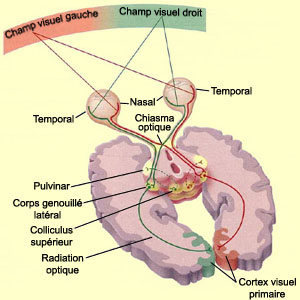
\includegraphics[width=0.4\textwidth]{figures/ch3_1_colliculus}\\

  \caption{ Position des deux colliculus dans le circuit visuo-moteur.}
  \label{fig: coll}
\end{figure*}

Afin d'éclaicir les mécanismes assurant la corrélation entre cette structure du cerveau et sa fonction visuo-motrice, plusieurs modèles du \gls{sc} ont été proposés  \cite{VanGisbergen:1985, Scudder:1988, Droulez:1991, Arai:1994,Nichols:1995, Breznen:1997, Lefevre:1998, Findlay:1999, Gancarz:1999, Short:2001, Trappenberg:2001, Badler:2002, Goossens:2006, Nakahara:2006, Marino:2008, Marino:2012} permettant de simuler numériquement plusieurs caractéristiques du comportement visuo-moteur et de ses circuits neuronaux fondamentaux.\\


La plupart de ces modèles ont été conçus pour aborder des questions spécifiques (comportement ou proprieté) basées sur différents mécanismes et jusqu'à aujourd'hui il reste très difficile d'avoir une vision synthétique qui caractérise clairement la contribution du \gls{sc} à la génération des saccades visuelles aussi bien au niveau électrophysiologique qu'au niveau comportemental. Un modèle complet  comprenant tous ces mécanismes pourrait peut être entièrement expliquer comment cette structure contribue à la génération des saccades mais assembler ces modèles est hors de portée parce qu'ils ne sont, pour la plupart, pas compatibles les uns avec les autres. Ils sont fondés sur différentes hypothèses liées à l'architecture, aux afférences ou aux caractéristiques fonctionnelles pour expliquer les mêmes phénomènes.\\

Nous avons donc décidé d'identifier les caractéristiques communes à ces modèles pour établir une proposition d'un modèle minimaliste. Ce modèle prend en compte les proprietés de base bien reconnues, principalement la représentation log-polaire de la surface rétinienne dans les couches profondes du \gls{sc} \cite{Ottes:1986}, le profil de connectivité latérale dans le \gls{sc} et la dynamique de l'activité de neurones colliculaires. Le modèle résultant est inévitablement beaucoup plus simple que les autres modèles déjà proposés. Cependant, nous rapportons un grand ensemble de résultats que nous avons pu reproduire et qui ont été souvent exploités pour valider des modèles beaucoup plus complexes. Nous proposons ici que des hypothèses plus simples sont suffisantes pour expliquer ces résultats et que beaucoup de propriétés émergent simplement des caractéristiques locales et bien connues.\\
%%%%%%%%%%%%%%%%%%%

Nous allons d'abord passer en revue quelques modèles déjà existants pour détailler ensuite les hypothèses que nous avons retenues. Sur la base de ces hypothèses, nous présentons dans la section des résultats un certain nombre de propriétés émergentes telles que le codage par population, la latence des saccades et la reproduction d'autres observations classiques électrophysiologiques et comportementales. En particulier, ce modèle offre un paradigme de sélection basé uniquement sur l'architecture intrinsèque. Enfin nous discuterons les principaux résultats de cette approche de modélisation.\\
%%%%%%%%%%%%%%%%%%%%%%%%%%%%%%%%%%%%%%%%%%%%%%%%%%%%%%%%%%%%%%%%%%%%%%%%%%%%%%%%%%%%%%%%%%%%%%%%%%%%%%%%%%

\section{Modèles de colliculus}

Chez les mammifères, le \gls{sc} est considéré comme une structure clé impliquée dans l'attention visuelle et le déclenchement de saccades \cite{Isa:2002}. D'une part, le \gls{sc} a été d'abord décrit comme une interface de transformation de signaux sensoriels en commandes motrices. Il reçoit les signaux rétiniens dans ses couches superficielles et renvoie à travers ses couches profondes prémotrices des ordres vers la formation réticulée [\gls{rf}]. D'autre part, cette structure participe également à des comportements plus complexes qui impliquent la sélection des cibles potentielles sur la base de facteurs exogènes et endogènes \cite {Kramer:1999}. Le \gls{sc} est donc considéré comme une importante structure d'intégration visuo-motrice. De nombreux modèles ont étudié ses propriétés physiologiques et comportementales (voir \cite {Girard:2005} pour une revue), ainsi que les différents flux d'information impliquant les couches colliculaires.  \\

\subsection{Intégration sensorimotrice}

Le colliculus supérieur agit comme un site d'intégration sensorimotrice, en recevant, entre autres, des entrées somato-sensorielles, auditives, ainsi que des signaux visuels\cite{Nolte:1993}. Ses entrées visuelles arrivent, soit directement de la rétine, soit par l'intermédiaire du cortex (modulées par l'intervention d'autres structures), pour fournir en sortie des prévisions des déplacements désirés à transmettre aux muscles oculaires via les neurones moteurs\cite{Wurtz:1996,Nolte:1993,Ursino:2009}. \\

En effet, la couche superficielle du colliculus supérieur est une couche visuelle qui reçoit des informations directement des cellules ganglionnaires de la rétine. Chaque site de cette couche s'active de façon optimale pour un stimulus présent en un point particulier du champ visuel. De son côté, la couche profonde forme une carte motrice topographiquement organisée : les vecteurs de la saccade résultante d'un stimulus visuel varient selon la position du stimulus. La correspondance entre les deux cartes fait penser à un mécanisme simple pour guider les yeux: un stimulus visuel projeté sur la rétine entraîne l'activation de la carte visuelle qui excite directement la carte motrice qui à son tour prépare l'ordre moteur permettant le déplacement désiré.\\

Ce modèle simple a été proposé dès 1970 suite à la découverte des cartes colliculaires. A l'époque, il était difficile de prouver l'existence des connexions descendantes directes entres les couches et de plus, il a été montré que les saccades n'exigent pas l'existence d'un stimulus visuel (saccades spontanées dans l'obscurité). Par la suite, ce modèle a été restreint aux saccades réflexes à très courte latence (saccades express) après avoir montré l'existence d'une connexion anatomique directe. Pour les saccades à plus grande latence, les chercheurs se sont dirigés vers des modèles qui intègrent des voies indirectes en passant par le cortex et les structures sous-corticales\cite{Wurtz:1996,Purves:2005}.\\ 

La structure du modèle décrit dans \cite {Findlay:1999} souligne que la principale tâche est de décider quand et où la saccade doit être effectuée. En conséquence, deux axes hiérarchiques sont définis. L'axe ``quand?'' (correspondant à \gls{fef}) décide du moment de quitter le point de fixation courant, alors que l'axe ``o\`u'' (correspondant au \gls{sc}) met en œuvre une compétition spatiale entre les cibles candidates. Un modèle combinant le \gls{fef} et le \gls{sc} a également été proposé dans \cite {Kramer:1999}, pour expliquer l'intégration d'éléments exogènes (stimuli externes en provenance de la rétine et des éléments endogènes (internes ou consignes élaborées dans le cortex préfrontal). \\

Plus tard, \cite {Godijn:2002} ont proposé un modèle computationnel d'intégration fondée sur de solides preuves expérimentales au niveau comportemental, qui suppose que tous ces éléments (traitement spatial, traitement temporel, stimuli exogènes et stimuli endogènes) peuvent être intégrés dans une seule carte, considérée comme un modèle du \gls{sc}. Il décrit donc le \gls{sc} comme une structure multimodale.\\

Cette carte inclut également des propriétés généralement considérées comme physiologiquement plausible: une excitation locale permettant de combiner des stimuli proches et un mécanisme d'inhibition plus large permettant de déclencher une compétition entre les stimuli éloignés \cite {VanOpstal:1989, Tweed:1990, Munoz:1998}. Ce schéma d'interaction explique pourquoi il a été possible d'utiliser un formalisme de champs neuronaux dynamiques [\gls{dnf}] \cite {Amari:1977} utilisé aussi dans \cite {Trappenberg:2001, Schneider:2002, Badler:2002,Marino:2012}. \\


D'autres études plus spécifiques proposent des éléments de la connectivité intrinsèque, afférente et efférente du \gls{sc}. C'est par exemple le cas pour la définition de plusieurs types de comportements neuronaux liés à différentes étapes de sélection de la cible \cite{Wurtz:1994} (\ref{typ}) et l'impact de la rétinotopie de projections visuelles sur la nature du traitement colliculaire \cite{Trappenberg:2001, Schneider:2002,Godijn:2002} (\ref{retin}) pour permettre d'évaluer le rôle de l'activité colliculaire dans l'encodage des saccades (\ref{eval}).




\subsection{Typologie neuronale}{\label{typ}}

La typologie des neurones colliculaires a été largement étudiée \cite {Wurtz:1994, Moschovakis:1996}. Il en résulte de nombreux modèles du colliculus supérieur sur des populations hétérogènes de neurones avec des dynamiques complexes. La plupart des modèles récents donnent un rôle plus important au \gls{sc} au prix d'un fonctionnement interne plus complexe. En effet, ces modèles définissent plusieurs types d'unités, en fonction de leur emplacement sur la carte, ce qui n'est pas très compatible avec le principe d'homogénéité dans les \glspl{dnf}. Wurtz et Optican ont proposé un modèle du \gls{sc} organisé en modules verticaux selon trois classes de neurones \cite{Wurtz:1994} : les neurones de fixation (FN), les neurones \textit{burst} (BN) et les neurones \textit{build-up} (BUN). La classification est faite en se basant sur des critères décrits précédemment dans \cite {Goldberg:1972,Munoz:1993a,Dorris:1997,Munoz:1995a}. \\



Par exemple, pour être classé comme un build-up, un neurone doit être situé entre 1 à 3 mm au-dessous de la surface dorsale du colliculus supérieur, doit commencer à décharger à une faible fréquence après le signal de déclenchement d'une saccade et doit continuer sa décharge jusqu'à la fin de la saccade \cite{Munoz:1995a,Dorris:1997}. \\



Cette classification reste une hypothèse permettant de définir plusieurs modèles de contrôle saccadique \cite{Trappenberg:2001, Schneider:2002}. Dans \cite {Godijn:2002} aussi, le substrat de calcul n'est pas homogène car la sensibilité des unités diminue avec leur excentricité sur la carte. Cette astuce est utilisée pour reproduire l'observation que la latence d'une saccade vers une cible, présentée conjointement avec un élément de distraction, est plus longue lorsque le distracteur est plus proche de la zone rostrale du \gls{sc} (correspondant à la fovéa).\\ 

Mais certains chercheurs optent plutôt pour une seule population homogène de cellules colliculaires qui change de comportement en fonction des paramètres extérieurs et des conditions expérimentales \cite {Trappenberg:2001, Droulez:1991}. Certaines études défendent l'existence d'une continuité entre les neurones de fixations et les autres neurones (appelés ``neurones de saccades'') \cite{Munoz:1995a}.\\


\subsection{Carte colliculaire topographique} {\label{retin}}

Les relations de voisinage spatial que les cellules ganglionnaires entretiennent entre elles au sein de la rétine, sont préservées au niveau de leurs cibles  corticales et sous-corticales. Les structures visuelles centrales présentent donc une représentation ordonnée de l'espace visuel \cite{Purves:2004}.\\

Au sein des aires visuelles primaires, la fovéa est représentée proche du pôle occipital, alors que les régions périphériques sont projetées sur les parties plus antérieures de la surface corticale. Les projections des excentricités sont donc encodées dans la direction postéro-antérieure (rostro-caudale). En outre, la carte rétinotopique est souvent déformée, ceci est lié au fait que l'espace visuel n'est pas uniformément échantillonné au niveau de la rétine.\\

Pour analyser la rétinotopie de manière quantitative, les modélisateurs définissent un système de coordonnées dans le champ visuel. Les coordonnées les plus adaptées au système visuel sont les coordonnées polaires $(\rho,\phi)$. On caractérise alors une position dans le champ visuel par son excentricité $\rho$ par rapport au centre du regard et par son angle polaire $\phi$, mesuré par exemple par rapport au méridien vertical inférieur. \\

Ensuite une carte rétinotopique est souvent approchée par une transformée log-polaire de l'image rétinienne \cite{Robinson:1972}. Le modèle le plus utilisé pour effectuer la transformation des coordonnées polaires du stimulus visuel sur la rétine en coordonnées cartésiennes sur le colliculus supérieur est celui proposé par \cite{Ottes:1986}.\\

Il s'agit d'un modèle quantitatif de la structure des cartes colliculaires basé sur la cartographie (mapping) obtenue expérimentalement par \cite{Robinson:1972} en stimulant électriquement le colliculus chez le singe. Il propose une fonction de projection logarithmique qui assure la projection des coordonnées rétiniennes en coordonnées colliculaires. Les équations de cartographie résultantes ont été ensuite utilisées dans plusieurs modèles \cite {VanGisbergen:1987,Optican:1995, Trappenberg:2001, Lefevre:1998, Marino:2008, Nakahara:2006}.\\
%En utilisant ce modèle, la rétine peut être réduite à la couche de photo-récepteurs.  

\subsection{\'Evaluation de l'activité colliculaire} {\label{eval}}

La plupart des modèles de génération de saccades supposent que les trajectoires des saccades sont stéréotypées. La vitesse et l'amplitude des saccades sont déterminées par l'activation d'une sous-population de neurones du colliculus supérieur profond \cite{Sparks:1990}. Mais des données expérimentales ont montré que les saccades ont des trajectoires assez variables \cite {Erkelens:1995}. Dans ces modèles de générateurs de saccades, différentes hypothèses ont été faites sur la nature des signaux codés au sein de l'activité colliculaire, i.e. la taille de la saccade désirée ou l'erreur motrice \cite{Waitzman:1988}. \\
%%%MOving hill"

Plusieurs modèles basés principalement sur des expériences sur le chat, supposent que les saccades sont initiées par une activité neuronale colliculaire qui se déplace au cours de la saccade de la zone caudale (périphérique) vers la zone rostrale (fovéale). Le but est d'amener l'activité résultant d'une stimulation vers la zone de fixation correspondant à la projection de la zone fovéale \cite {Droulez:1991, Lefevre:1992, Optican:1994 , Massonne:1994, Wurtz:1994, Schierwagen:1996, Grossberg:1997}. Cette hypothèse n'est plus supporté, certaines études sur les singes ont montré l'inexistence de cette translation d'activité \cite{Robijanto:2002}. L'activité neuronale pendant les saccades est plutôt considérée stationnaire et stéréotypée comme spécifié dans \cite {Anderson:1998}.\\
%%%%SStériotypée

Le modèle proposé dans \cite{VanOpstal:2008} suppose que la forme et la taille de la sous-population colliculaire activée par un stimulus visuel sont invariantes pour toutes les saccades et que cette sous-population active peut être décrite par un profil gaussien d'une largeur fixe et un maximum de fréquence moyenne de décharge. Ce modèle récent est basée sur une formulation mathématique et produit des résultats satisfaisants, mais il n'aide pas à comprendre la structure du colliculus supérieur et des connexions possibles incluses dans le contrôle du regard. Il s'agit d'imposer certaines propriétés qui sont censées être des fonctions émergentes, c'est pourquoi des modèles computationnels à base de réseaux neurones nous semblent plus appropriés à la compréhension du lien entre la structure et ses fonctions.\\
%%%décodage

De nombreux schémas de décodage de l'activation colliculaire ont été proposés \cite {McIlwain:1976, Sparks:1976, Massonne:1994, Badler:2002, Lee:1988, Bozis:1998}. Plusieurs schémas d'évaluation de la sortie du \gls{sc} ont été proposés. Le schéma le plus simple est celui du \textit{winner-takes-all} où le site le plus actif impose la direction, en supposant que chaque site code pour une direction. Ensuite, deux schémas de calcul sont souvent proposés dans les modèles de décodage de l'activité colliculaire:\\

\begin{itemize}

\item le vecteur moyenne \cite {Lee:1988} basé sur une normalisation qui dépend du nombre de neurones actifs. Dans ce schéma de décodage, on parle plutôt de la ``contribution'' $\vec{R}_n$ d'une cellule $n$ au vecteur de mouvement (déplacement) \cite{Walton:2005, Lee:1988}. La somme correspond donc à l'addition des contributions de toutes les cellules de la population. Le vecteur déplacement $\vec{S}$ vers la cible de la saccade est calculé en fonction des fréquences de décharges moyennes $r_n$ comme suit:

\begin{align}
  \vec{S} = \frac{\sum_{n=1}^{N} r_n\vec{R}_n }{\sum_{n=1}^{N} r_n}
\label{moy}
\end{align} 

\item le vecteur somme \cite{McIlwain:1976, Sparks:1976} où toutes les activités des neurones colliculaires sont additionnées avec des pondérations fixées selon la position sur la carte. Dans ce schéma de décodage, on désigne une ``direction préférée'' pour chaque cellule. Plus généralement, à chaque cellule correspond un champ de mouvement qui correspond à l'ensemble des directions pour lesquelles cette cellule s'active. Si on utilise le décodage par somme, il faut définir la contribution de chaque cellule dans le mouvement définie comme l'amplitude caractéristique divisée par la taille de la bulle d'activité. Cette bulle d'activité est supposée avoir une amplitude constante indépendamment de sa position. La contribution $\vec{m}_n$ d'un neurone $n$ est une grandeur caractéristique du neurone indépendante de son activation. Le vecteur déplacement est calculé comme suit: 

\begin{align}
  \vec{S} = \sum_{n=1}^{N} r_n\vec{m}_n 
\label{moy}
\end{align} 

\end {itemize}

\begin{figure}[ht]
  \begin{center}
    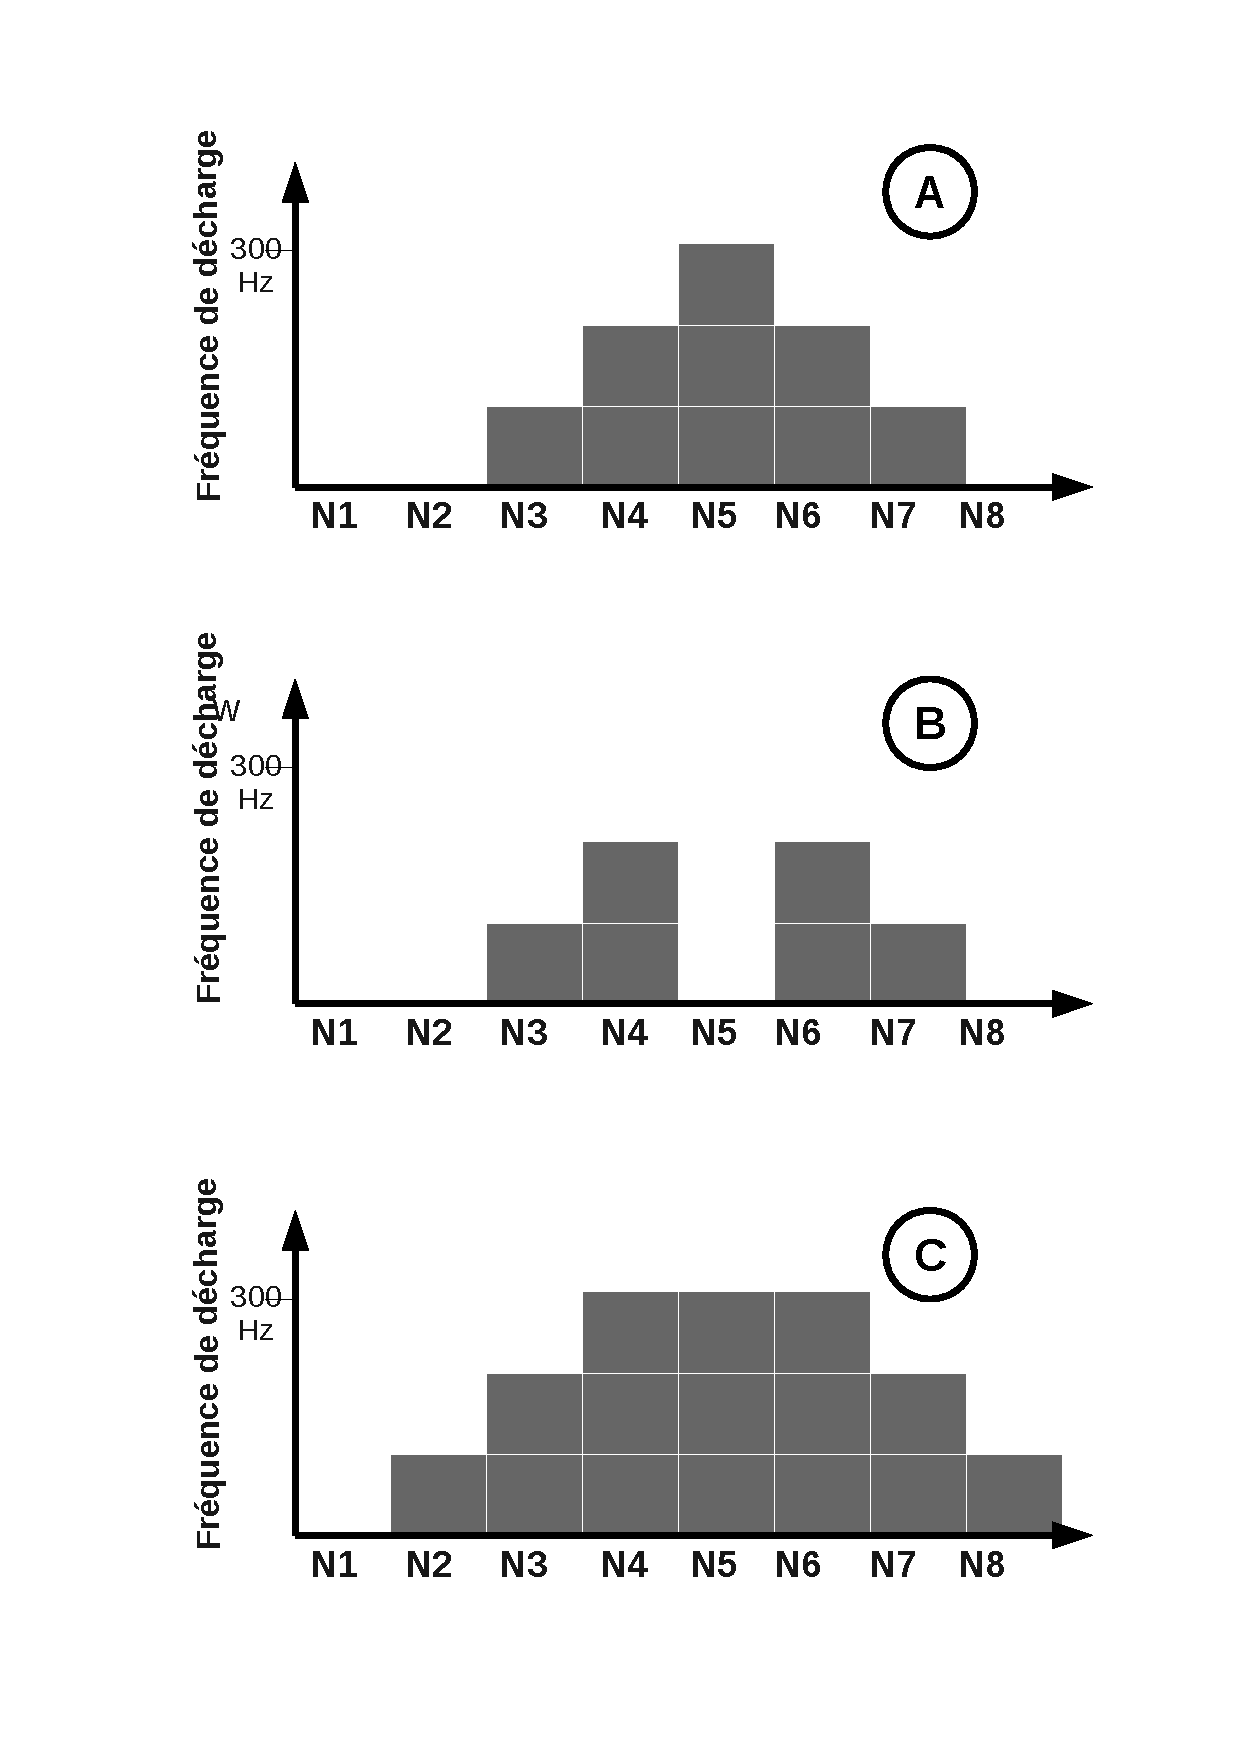
\includegraphics[width=0.6\textwidth,height=10cm]{figures/ch3_2_sum-average}
  \end{center}
  \caption{ Exemple théorique illustrant la différence entre les schémas de décodage de l'activation colliculaire sur une carte supposée linéaire: A- Cas normal, B- Inhibition partielle de la zone active C- Sur-activation. Les diagrammes correspondent aux fréquences de décharge d'une population de neurones $Ni$, $i\protect\in[1..8]$, en prenant en compte leur disposition spatiale. Les neurones N4 et N6 sont par exemple les voisins immédiats du neurone N5.}
  \label{sumav}
\end{figure}

Considérons un exemple simple illustré par la figure (fig.\ref{sumav}-A). On considère que la direction préférentielle d'un neurone $N_i$ se situe à une amplitude $i$. Le neurone N5 étant le plus activé, s'il décide tout seul, la saccade correspondant à ce profil d'activation serait d'une amplitude de 5°. Le décodage par moyenne et le décodage par somme donnent la même valeur (5) dans le cas normal\footnote{
\textit{L'amplitude désirée selon le décodage par moyenne}\\
\textit{= la somme des directions pondérées par les activations/ somme totale des activations }\\
                     $=(0+0+100*3+200*4+300*5+200*6+100*7+0)/(100+200+300+200+100)=5$\\

Si on considère un décodage par somme, on définit les contributions des neurones. La contribution du neurone N2, par exemple, $vaut 2/900=0.00222$. La contribution du neurone N2, par exemple, $vaut 2/900=0.00222$. D'o\`u:\\

\textit{L'amplitude désirée selon le décodage par somme}\\
\textit{= la somme des contributions des cellules de la population active pondérée par leurs activations}\\
                     $=(0+0+100*3/900+200*4/900+300*5/900+200*6/900+100*7/900+0)=5$\\}.\\

Ces deux modes d'évaluation sont équivalents dans le cas d'une population saine activée normalement (pas de lésions) mais peuvent différer en cas d'inactivation (par injection de substances inhibitrices par exemple) ou de sur-activation (par stimulation électrique par exemple). Prenons les cas illustrés par les figures (fig.\ref{sumav}-B, fig.\ref{sumav}-C).\\

La figure B correspond à une lésion, le calcul de la moyenne donne une amplitude de $5$ mais le calcul de la somme donne une amplitude de $3.33$. De même dans le cas d'une sur-activation, la figure C, les résultats ne sont pas convergents, avec le vecteur somme on obtient $8.33$ et avec le vecteur moyenne on obtient $5$.\\

Ces schémas sont considérés d'un point de vue ``statique'' en supposant que le colliculus supérieur n'est pas inclus dans la boucle de feedback moteur contrairement à ce que proposent plusieurs modèles \cite{Robinson:1972}. L'activité du colliculus est supposée coder le déplacement désiré et non-pas l'erreur motrice instantanée (ce qui reste à l'oeil à parcourir pour arriver au but). \cite{Gandhi:2011} introduisent un troisième schéma qui décode l'activité au fur et à mesure que l'activité évolue qu'on ne détaillera pas ici.\\

Certaines expériences ont donné des résultats en faveur de la moyenne \cite{Lee:1988}, d'autres plutôt en faveur de la somme sans donner une synthèse concluante. Le problème est que ces expériences restent compliquées et non maîtrisées (le dosage, la diffusion, la précision de l'injection, les neurones affectés...) et difficilement reproductibles.\\

Nous détaillerons dans la section suivante les hypothèses que nous avons retenues de tous ces modèles pour proposer un modèle minimaliste permettant de reproduire et d'expliquer un certain nombre de résultats d'expériences biologiques décrits et discutés dans la suite.\\
%\subsection{Synthèse}
%{\scriptsize
%\begin{tabular}{|c|c|c|c|c|c|c|c|c|}
%\hline
%	& {\em Connectivité} & {\em Typologie} &{\em Mapping }&{\em Entrées}& {\em Sorties }& {\em Fonctions}\\
%	& {\em latérale}  & {\em neuronale}  &        {\em }&{\em Stimulus}& {\em Décodage }& {\em Dynamique}\\
%\hline
%\cite{Tabareau:2006}&           &	BN/BUN	&    linéaire             &			&           somme pondérée      & seulment BN 		\\
%&           &		&    ou log            &			&                 &	activité stéréotypée	\\
%\hline
%\cite{Stephan:2002}	&   inhib+excit & BUN   &                 &			&                 &	accumulation BUN \\

%	&                 &		BN &                &			&                 &	sélection BN		\\

%	&                 &		FN   &             &			&                 &		\\
%\hline
%\cite{Lee:1988}	&                 &		&                 &			&       vector sum           &		\\
%&                 &		&                 &			&      by ihibition          &		\\
%\hline
%\cite{Badler:2000}	&                 &		&                 &			& vector avg               &		\\
%\hline
%\cite{Anderson:1998}	& &   BUN/BN              &	log-polaire	                &			&                 &		\\
%\hline
%\cite{Wurtz:1994}	&                 & BUN/BN/FN	&                 &			&                 &stationnaire		\\%
%	&                 &		&                 &			&                 &/mouvante		\\
%\hline
%\cite{Opstal:2008}	&                 &		&                 &			&                 &	Math stéréotypée	\\
%\hline
%\cite{Goossens:2008}	&    non             &	non	&                 &	gaussienne		&    vector sum             &		\\
%\hline
%\end{tabular}
%}
%%%%%%%%%%%%%%%%%%%%%%%%%%%%%%%%%%%%%%%%%%%%%%%%%%%%%%%%%%%%%%%%%%%%%%%%%%%%%%%%%%%%%%%%%%%%%%%%%%%%%%%%%%%%%%%%%%%%%%%%%%%%%%%%%%%%%%%%%%%%%%%%%%%%%%%%%%%%%%%%%%%%%%%%%%%%%%%%%%%%
\section{Hypothèses et méthodes}

Nous avons simulé numériquement un modèle de réseau de neurones de trois couches organisées topologiquement en utilisant le formalisme de \textit{champs neuronaux dynamiques} [\gls{dnf}] décrit dans le premier chapitre \cite{Amari:1977}. La première couche correspond à la rétine et la deuxième couche correspond au colliculus supérieur profond. Une troisième couche intermédiaire est aussi utilisée qui peut représenter des structures intermédiaires telles que \gls{v1} et qui servira principalement à expliciter la déformation log-polaire (décrite dans la suite) de la projection de la carte rétinienne sur la carte colliculaire. D'un point de vue numérique, cette couche intermédiaire n'est pas indispensable, la projection peut se faire directement sur la carte colliculaire. Comme expliqué dans l'introduction, le modèle a été établi seulement sur la base des hypothèses communes à d'autres modèles du \gls{sc} que nous résumons dans les cinq points suivants:\\

\begin{itemize}

\item[$\bullet$] Un stimulus physique (une cible) est représenté sur la surface (correspondant à la rétine) par une petite activation gaussienne (à deux dimensions). La rétine est réduite donc à une couche de photorécepteurs et nous considérons que le niveau de l'activation de ces récepteurs est proportionnel à l'intensité de la lumière.\\

\item[$\bullet$] On suppose que le lieu de l'activation sur le \gls{sc} code l'emplacement de la cible dans le champ visuel et que cette activation est à l'origine de la saccade qui apportera l'image de la cible sur la fovéa (fovéation). Deux activations voisines dans la couche \gls{sc} correspondent à des localisations de cibles voisines dans le champ visuel (codage topographique) \cite{Schiller:1972, Wurtz:1972}.\\

\item[$\bullet$] La projection du champ visuel sur la surface colliculaire est basée sur le modèle quantitatif de \cite{Ottes:1986} qui propose qu'une fonction de cartographie logarithmique assure la transformation des coordonnées rétiniennes en coordonnées colliculaires (une projection log-polaire). Nous supposons également que le stimulus est projeté en entier sur le \gls{sc} et non pas seulement son centre de masse.\\

\item[$\bullet$] Nous considérons le colliculus supérieur comme étant une carte homogène et uniforme d'unités neurales \cite{Trappenberg:2001,Droulez:1991}. En plus de ses afférences rétiniennes excitatrices, d'autres entrées excitatrices et inhibitrices latérales intracolliculaires qui dépendent de la distance entre les neurones sont considérées, comme proposé dans beaucoup de modèles \cite{Arai:1994, Droulez:1991, Gancarz:1999, Lefevre:1992, Optican:1995, Short:2001, Trappenberg:2001, Nakahara:2006}.\\

\item[$\bullet$] Les influences des aires corticales, des ganglions de la base et du cervelet sur l'activité colliculaire ne sont pas considérées ici.(sauf que l'inhibition latérale pourrait correspondre à une entrée inhibitrice de \gls{bg} (\gls{gpi}), comme proposé dans plusieurs papiers \cite{Trappenberg:2001})\\

\item[$\bullet$] Un seul colliculus est considéré.\\
\end{itemize}
L'architecture globale du modèle est donnée par la figure \ref{archi}.
\begin{figure}[ht]
  \begin{center}
    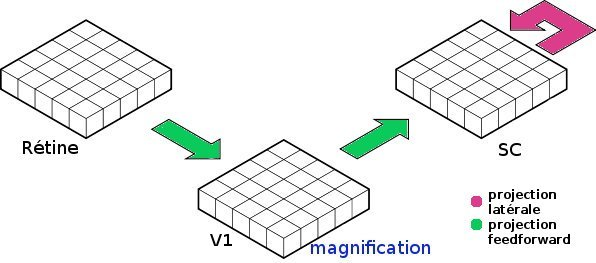
\includegraphics[width=0.7\textwidth]{figures/ch3_3_model0}
  \end{center}
  \caption{ Architecture du modèle. Une carte d'entrée représentant une demi rétine. Une carte intermédiaire (V1) représentant la projection rétinotopique. Une carte de sortie représentant la couche pré-motrice du colliculus supérieur }
  \label{archi}
\end{figure}
\subsection{L'entrée rétinienne}

 L'hémichamp visuel $V$ $[0^\circ,90^\circ]\times[-90^\circ,90^\circ]$ est projeté sur l'espace continu $R$ $[0,1]\times[-1,1]$ correspondant à la moitié d'une rétine. N'importe quel stimulus $S$ présenté dans $V$ aux coordonnées polaires $(\rho_s,\phi_s)$ (en degrés) est projeté sur $R$ aux coordonnées cartésiennes $(u_s, v_s)$. Nous avons considéré des stimuli ronds avec une distribution gaussienne de la luminosité tels que l'activité $U_r (u, v)$ en un point $(u, v)$ de $R$ en présence d'un stimulus S est donnée par l'équation suivante :\\

\begin{align}
  U_r(u,v)= C~exp\left(-\frac{\vert u - u_s\vert^2 + \vert v - v_s \vert^2}{2{\sigma_c}^2}\right)
\end{align}

en supposant que $(u_s, v_s)$ est le centre de la projection du stimulus sur la carte R, $\sigma_c$ est la taille angulaire du stimulus et $C$ est l'activation maximale dans $R$ (correspondant à l'intensité maximale du stimulus). Les stimulus sont supposés avoir approximativement un diamètre angulaire de 1° dans la rétine, qui correspond à $\sigma_c=1/90$.\\

\subsection{La projection visuelle sur le colliculus supérieur profond }

Selon la description de \cite{Robinson:1972}, la projection de $R$ sur le \gls{sc} est approximée en utilisant une transformation log-polaire, qui réduit le modèle de \gls{sc} à une carte bi-dimensionnelle. Une approximation mathématique de cette transformation a été proposée par \cite{Ottes:1986}. Il s'agit de la projection standard utilisée dans la plupart des modèles computationnels du colliculus \cite{Optican:1995, Trappenberg:2001, Lefevre:1998, Marino:2008, Nakahara:2006} :

\begin{align}
  x &=
  B_x~log\left(\frac{\sqrt{\rho^{2}+2A\rho|\cos{(\phi)}|+A^{2}}}{A}\right) \notag \\
  y &=
  B_y~arctan\left(\frac{\rho \sin{(\phi)}}{\rho|\cos{(\phi)}|+A}\right)
  \label{eq: mapping}
\end{align}

où $(x,y)$ représentent les coordonnées cartésiennes dans le \gls{sc} (en millimètres), $(\rho,\phi)$ les coordonnées polaires dans $R$ (en degrés). $Bx$ (en millimètres) est une constante déterminant la taille de la carte colliculaire le long de l'axe horizontal. $By$ (en millimètres) est une constante déterminant la taille de la carte colliculaire le long de l'axe vertical. $A$ (en degrés) est une constante qui (avec le rapport $Bx/By$) détermine la forme de la carte. Un stimulus à $\rho=90°$ et à $\phi=-90°$ active une cellule à $x=4,8mm$ (correspondant à la longueur réelle d'un colliculus chez le singe) et à $y=-2,76mm$ (correspondant à la moitié de sa largeur réelle) \cite{Ottes:1986}. Cette transformation log-polaire amplifie la représentation de la région fovéale comme le montrent les figures \ref{fig: mapping}-A et \ref{fig: mapping}-D dans la suite.\\


\begin{figure}
\begin{tabular}{|c|c|}
\hline
A&B\\

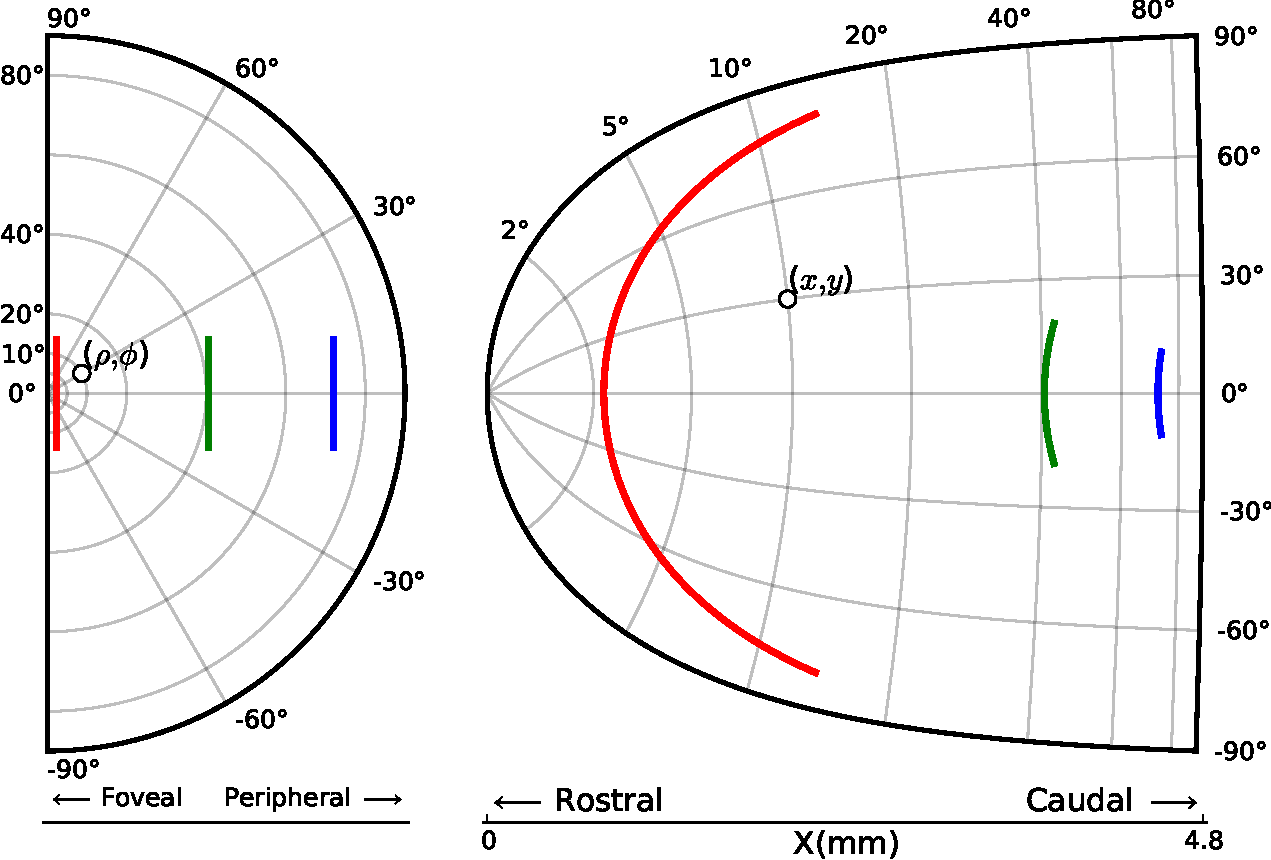
\includegraphics[width=.5\textwidth]{figures/ch3_4_mapping} & 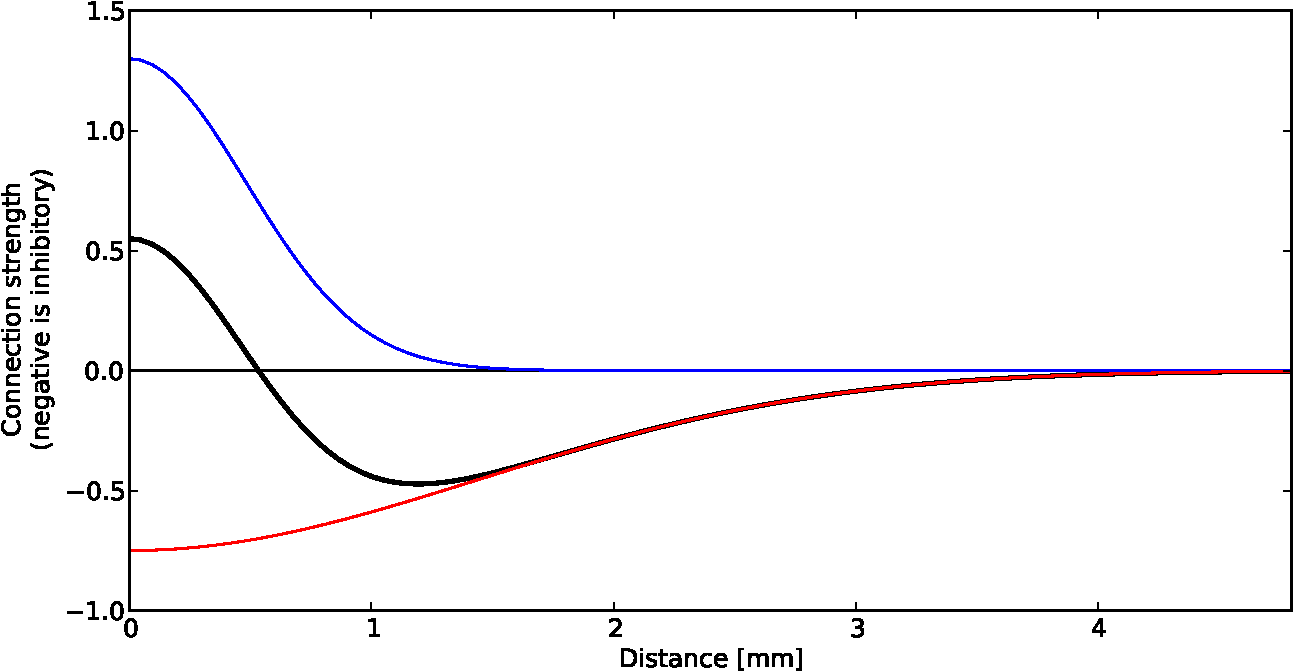
\includegraphics[width=.5\textwidth,height=5cm]{figures/ch3_4_weights-profile}\\
\hline
C&D\\

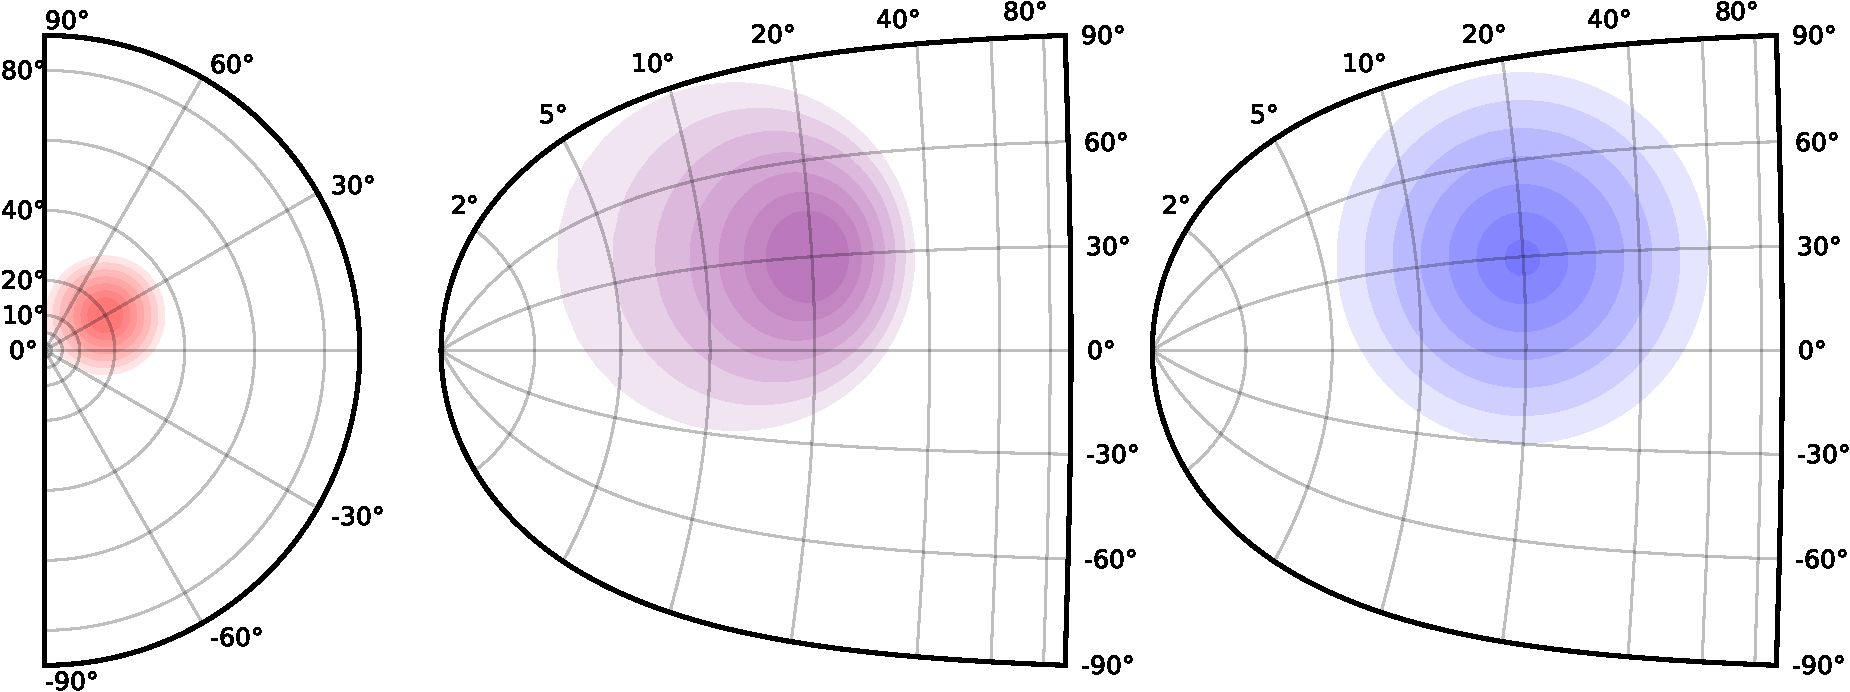
\includegraphics[width=.5\textwidth]{figures/ch3_4_topology}& 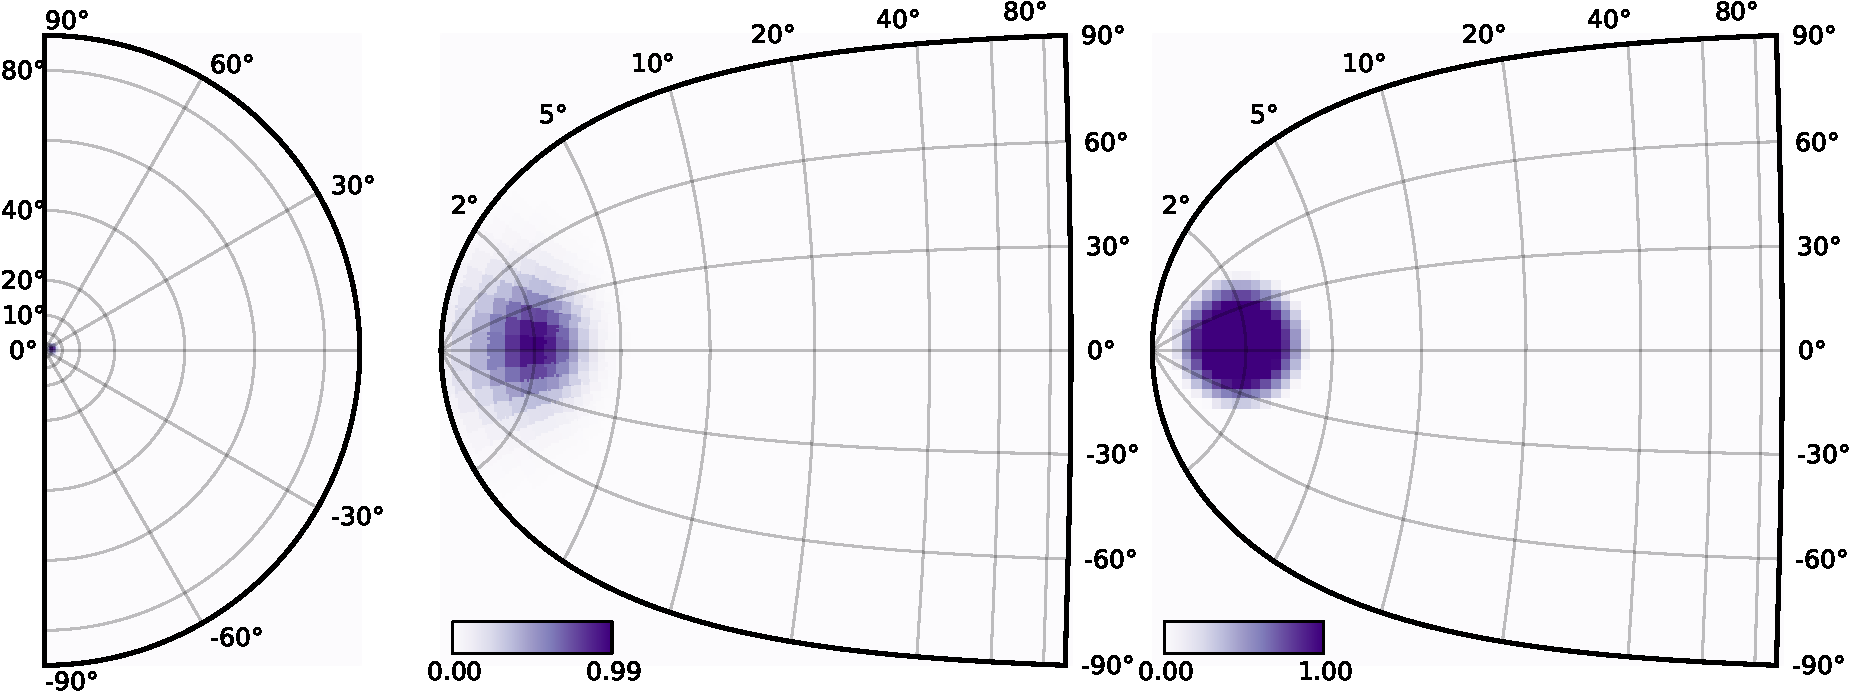
\includegraphics[width=.5\textwidth]{figures/ch3_4_stimulus-1}\\
\hline
\end{tabular}
  \caption{
Description du modèle. A. Projection des coordonnées polaires dans l'espace visuel en coordonnées cartésiennes dans le \protect\gls{sc}. La projection rétinotopique modifie les propriétés géométriques de l'image tout en gardant les relations de voisinage. \protect\`A gauche, l'hémichamp visuel droit (lignes des iso-directions et des demi-cercles d'excentricité constante). \protect\`A droite la carte représentant le colliculus avec des lignes d'iso-amplitudes du \protect\gls{sc} $(2° à 90°)$ et des lignes d'iso-directions $(- 90° à 90°)$ sont indiquées. Les coordonnées polaires visuelles $(\protect\rho, \protect\phi)$ sont transformées en coordonnées colliculaires cartésiennes $(x, y)$ en utilisant les équations \protect\ref{eq: mapping}. Les lignes colorées illustrent la magnification de la représentation des stimuli dans la région fovéale. B. Le pattern des connexions intracolliculaires (noires) résultant de la différence entre une fonction excitatrice locale (bleue) et une fonction inhibitrice globale (rouge). C. Relation topologique entre la surface rétinienne isotropique (rouge), les projections colliculaires anisotropiques correspondant à la présentation d'un stimulus dans le champ visuel (pourpre) et la connectivité latérale isotropique (bleue) dans le colliculus supérieur. D. La projection d'un stimulus visuel gaussien (situé à (2°,0°)). Au milieu, la projection d'entrée à la carte colliculaire. \protect\`A droite l'activité du colliculus supérieur enregistrée après stabilisation de son activité.
}
  \label{fig: mapping}
\end{figure}

En ce qui concerne les détails de la simulation, nous n'avons pas utilisé une fonction explicite du système inverse des équations \ref{eq: mapping} permettant de faire la projection des coordonnées rétiniennes en coordonnées colliculaire. Nous avons plutôt calculé une approximation numérique de la transformation inverse.

\subsection{La carte computationnelle du colliculus}

La couche profonde du \gls{sc} a été modélisée en utilisant la théorie des champs neuronaux dynamiques \cite{Amari:1977, Taylor:1999} décrite dans le premier chapitre selon laquelle un volume cortical donné Ω est considéré comme étant un continuum spatial. Bien que cette théorie ait été proposée pour simuler principalement des activités dans le cortex cérébral, nous avons supposé que la densité neurale dans le \gls{sc} est assez élevée pour nous permettre de transposer cette théorie, comme supposé dans plusieurs autres modèles \cite{Trappenberg:2001, Schneider:2002, Marino:2012}. Le formalisme des \glspl{dnf} propose que la population des unités neurales actives peut être décrite comme un champ continu d'activités. Les unités neurales, comme éléments de la carte, peuvent être considérées comme un ensemble de processeurs homogènes fonctionnant en parallèle sur les signaux entrants. La dynamique du champ est régie par une équation du type :

\begin{align*}
	\frac{1}{\tau} \frac{\partial u({ \vec{z}},t)}{\partial t}
	 = - u({\bf \vec{z}},t)
 	 + \int_{\Omega}^{} w({ \vec{z}},{\vec{z'}})f(u({ \vec{z'}}, t - \frac{|{ \vec{z}-\vec{z'}}|}{v}))d{\vec{z'}}
     + i({\vec{z}},t) 
\end{align*}


o\`u  $u(\vec{z}, t)$ représente l'activité (le potentiel moyen de membrane) à la position $\vec{z}$ à l'instant $t$, $I(\vec{z},t)$ représente l'entrée synaptique reçue à l'instant $t$ et à la position $\vec{z}$, $W$ est une fonction de poids décrivant la force de la connexion entre une unité neurale à la position $\vec{z}$ et une unité à la position $\vec{z'}$, $f$ est la fonction de fréquence de décharge d'une unité neurale simple, $v$ est la vitesse de conduction d'un potentiel d'action et $\tau$ est une constante de temps caractéristique de l'activation des neurones. \'Etant donnée la petite taille du colliculus , la vitesse de conduction a été négligée $(v=+\infty)$ et le champ de l'activité colliculaire a été considéré comme homogène et isotrope, ce qui mène à l'équation simplifiée suivante :\\
%1/τ (∂u (⃑ de z, t))/∂t=-u (⃑ de z, t)+∫_SC▒w (|^ de ⃑-z ⃑ de z ' |) f (u (⃑ de z, t)) DZ ⃑'+i (⃑ de z, t)    (5)
\begin{align}
	\frac{1}{\tau} \frac{\partial u({\vec{z}},t)}{\partial t}
	 = - u({ \vec{z}},t)
 	 + \int_{\Omega}^{} w(|{\vec{z}}-{\vec{z'}}|)f(u({\vec{z'}}, t))d{ \vec{z'}}
     + i({\vec{z}},t)
  \label{eq: neural_field}
\end{align}

Pour la fonction f de fréquence de décharge, nous avons employé une fonction simple $f(u)=min(max(u, 0), 1)$ \footnote{le 1 correspond à la fréquence de décharge maximale (qui sera considérée égale à 500Hz dans la simulation) } puisque c'est la fonction la plus simple qui peut fournir la stabilité pour un tel champ \cite{Salinas:1996}.\\

La densité des unités neurales dans le \gls{sc} est considérée constante le long de la surface colliculaire et nous considérons que la force des connexions latérales excitatrices et inhibitrices est représentée par une fonction qui dépend de la distance entre les cellules mesurées sur la surface du \gls{sc} i.e. [$ w(\vec{z},\vec{z'})=w(\vert \vec{z}-\vec{z'} \vert)$]. La connectivité latérale d'une cellule donnée est ainsi isotrope (fig \ref{fig: mapping}-C), contrairement à \cite{Nakahara:2006} où les connexions sont basées sur la proximité des stimuli. Considérons deux cellules à deux positions respectives $\vec{z}$ et $\vec{z'}$, la force de connexions résultante est définie par:\\

\begin{align}
w(\vec{z},\vec{z'})=E~exp\left(-\frac{\vert \vec{z}-\vec{z'} \vert^2}{{\sigma_e}^2}\right) -
  I~exp\left(-\frac{\vert \vec{z}-\vec{z'} \vert^2}{{\sigma_i}^2}\right)
  \label{eq: weight}
\end{align}

o\`u $E$, $I$ sont les amplitudes, $\sigma_e$, $\sigma_i$, sont respectivement les écarts types des fonctions gaussiennes excitatrices et inhibitrices. Nous avons considéré pour nos simulations $\sigma_i \gg \sigma_e$, ce qui correspond à des connexions inhibitrices à longue portée (globales) et des connexions excitatrices à courte portée (locales).\\

Les effets de l'inactivation locale dans le \gls{sc} ont été simulés numériquement en multipliant la matrice d'activation $U$ résultant de l'équation (eq \ref{eq: neural_field}) par une matrice binaire $L$ (un masque) dans laquelle un état d'activation est attribué à chaque unité ($1$ pour une unité d'active et $0$ pour inactivée). Dans les expériences, le modèle de lésion que nous employons est une matrice avec un disque uniforme de valeurs nulles.\\

\subsection{Le d\'ecodage de l'activité colliculaire}

Comme passé en revue dans \cite{Gandhi:2011}, plusieurs schémas de décodage de l'activité du \gls{sc} ont été proposés.  Sauf indication contraire, le déplacement désiré de l'oeil $\vec{\Delta E}$  est décodé en utilisant un vecteur de moyenne statique:

\begin{align}
  \Delta\vec{E} = \frac{\sum_{\substack{\Omega}}^{} r_z\vec{R}_z }{\sum_{\Omega}^{}r_z}
\label{sommation}
\end{align}

avec $r_z$ est la fréquence moyenne de décharge d'une cellule à une position donnée $\vec{z}$ et $\vec{R}_z$  est le vecteur de déplacement préféré codé par cette cellule. Nous n'avons pas choisi le schéma de décodage par somme car l'activation obtenue n'est pas parfaitement stéréotypée, le nombre d'unités actives en réponse à un stimulus est constant mais l'activation maximale varie selon l'excentricité. \\


\section{Résultats}

\subsection{\' Etendue de la population active}

Nous avons examiné l'étendue de la population active dans la carte du \gls{sc} qui résulte de la présentation de stimuli identiques à différents emplacements du champ visuel. L'entrée de la carte colliculaire est différente pour chaque stimulus en raison de la déformation logarithmique (fig \ref{fig: mapping}-C et \ref{fig: mapping}-D). En effet, à cause de la projection non linéaire de la carte rétinienne sur la carte du \gls{sc}, un stimulus apparaissant dans le champ visuel central\footnote{On distinguera dans les descriptions des positions des stimuli, les stimuli centraux correspondant à des projections fovéales sur la rétine et rostrales sur le colliculus et les stimuli périphériques correspondant à des projections périphériques sur la rétine et caudales sur le colliculus} active initialement une population d'unités neurales colliculaires plus grande que celle activée par des stimuli plus périphériques. Cependant, après plusieurs pas de calcul, la distribution de l'activité colliculaire atteint un état stable ayant toujours la même forme et la même étendue spatiale de la population active, sans se soucier de l'excentricité de la cible dans le champ visuel. On parle donc d'une bulle d'activité ``stéréotypée'' (en étendue et non pas en amplitude à cause la décroissance de l'activation maximale des neurones avec l'excentricité comme montré dans la suite). Cet état final résulte du profil imposé à la connectivité latérale. La distribution de l'activité sur la carte se rapproche d'une gaussienne (2D) quand elle se stabilise. L'étendue de la connectivité excitatrice détermine la taille finale de la population active (puisque l'inhibition est supposée être globale). 

\subsection{Champs récepteurs}

Nous avons de même examiné la réponse des unités neuronales situées à différents emplacements dans la carte du \gls{sc} en réponse à des stimuli présentés à différentes excentricités dans la carte de la rétine. \\

\begin{figure}[ht]
  \begin{center}
    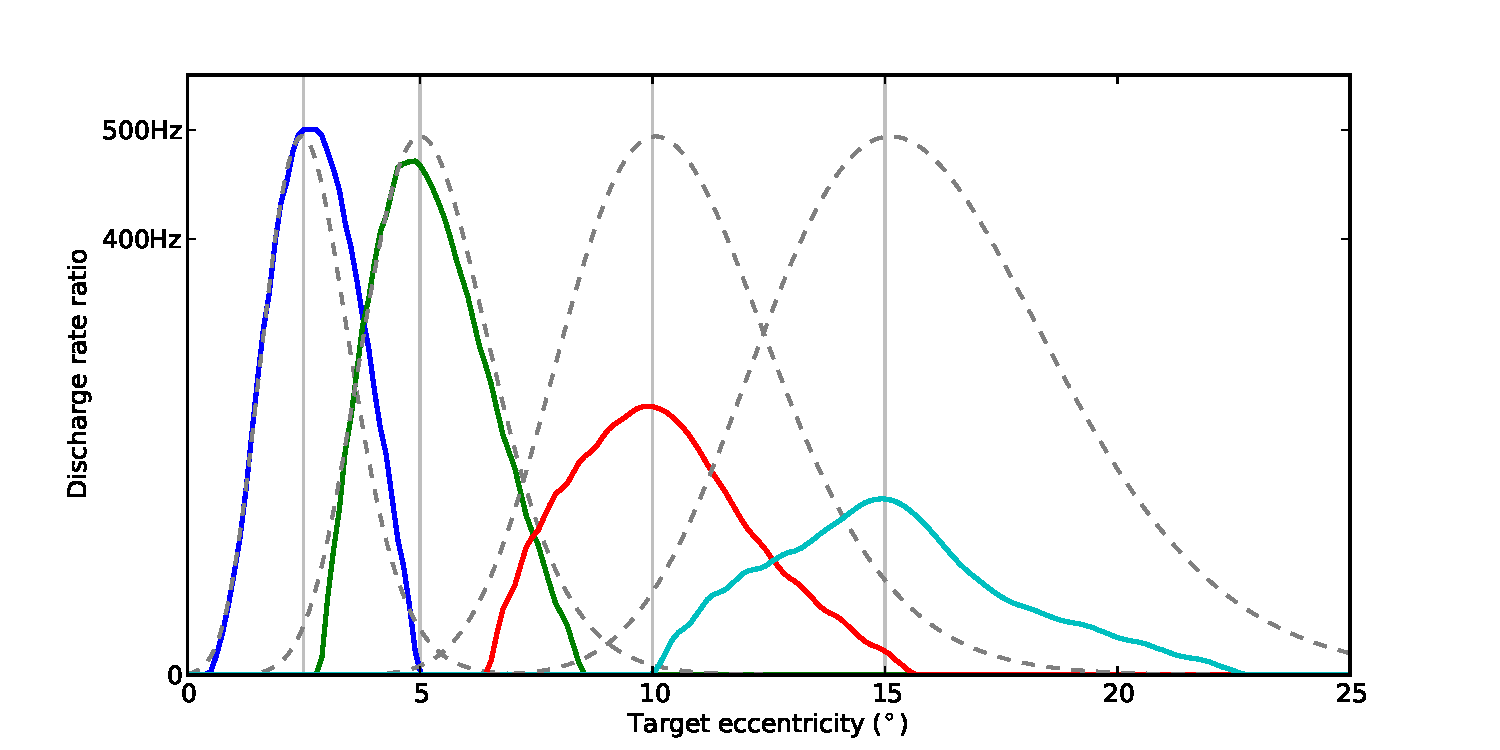
\includegraphics[width=0.8\textwidth]{figures/ch3_5_RF}
  \end{center}
  \caption{ Champs récepteurs. Réponse neuronale (4 neurones) à un stimuli présenté successivement à des excentricités variant de 1° à 25°. Pour chacun des 4 neurones (situés respectivement à une excentricité d'à peu près 2.5°, 5°, 10° et 15° et une amplitude de 0° pour tous sur la carte colliculaire selon la projection logarithmique). L'activation maximale (fréquence de décharge) est mesurée à la convergence du système. La largeur des champs récepteurs décroît avec l'excentricité. Les pointillés représentent les entrées (l'activation initiale).}
  \label{fig: receptive-field}
\end{figure}

La figure (fig \ref{fig: receptive-field}) montre que le champ récepteur\footnote{Le champ récepteur d'une cellule neuronale colliculaire est l'intervalle des excentricités des cibles pour lesquelles cette unité s'active} d'une unité dépend de l'emplacement de cette unité dans la carte colliculaire. La réponse est maximale pour une excentricité préférée, diminue en s'éloignant de part et d'autre de cette excentricité (c'est à dire diminue pour des excentricités plus petites ou plus grandes) et disparaît pour des saccades vers des emplacements qui sont relativement très loin de l'excentricité préférée. La forme des champs est un peu asymétrique et plus l'emplacement préféré est excentré, plus la courbe d'accord est large.

\subsection{Exactitude}

En utilisant le décodage par moyenne (eq \ref{sommation}), nous avons examiné l'exactitude (\textit{accuracy}) du modèle en présentant des cibles à divers emplacements dans le champ visuel. La figure (fig \ref{fig: accuracy}-A) montre, le long de la carte colliculaire, les emplacements théoriques des stimuli par des petits cercles pleins et les emplacements résultant du décodage par des petits cercles vides. Malgré la transformation log-polaire de la carte rétinienne et le codage distribué des localisations des cibles (plusieurs unités s'activent pour une cible donnée), l'exactitude du modèle est assez satisfaisante, la distance angulaire moyenne entre les emplacements théoriques et les emplacements décodés après une seconde de com vaut $3.10^{-3}$. Quand des stimuli ont été présentés dans la zone fovéale, le biais du décodage (le décalage entre les cercles vides et pleins) de la cible sur le \gls{sc} est dans le sens de la partie périphérique du champ visuel et inversement le biais est plus dirigé vers la partie centrale quand les mêmes stimuli sont présentés dans la zone périphérique. Les biais de position sont plus fréquents sur les bords du \gls{sc}, i.e. dans les régions colliculaires codant des cibles sur la fovéa ou sur le méridien vertical.


\begin{figure}
  \begin{center}
    \begin{tabular}[t]{cc}
     {\textsf {\textbf A}} &
      {\textsf {\textbf B}} \\
      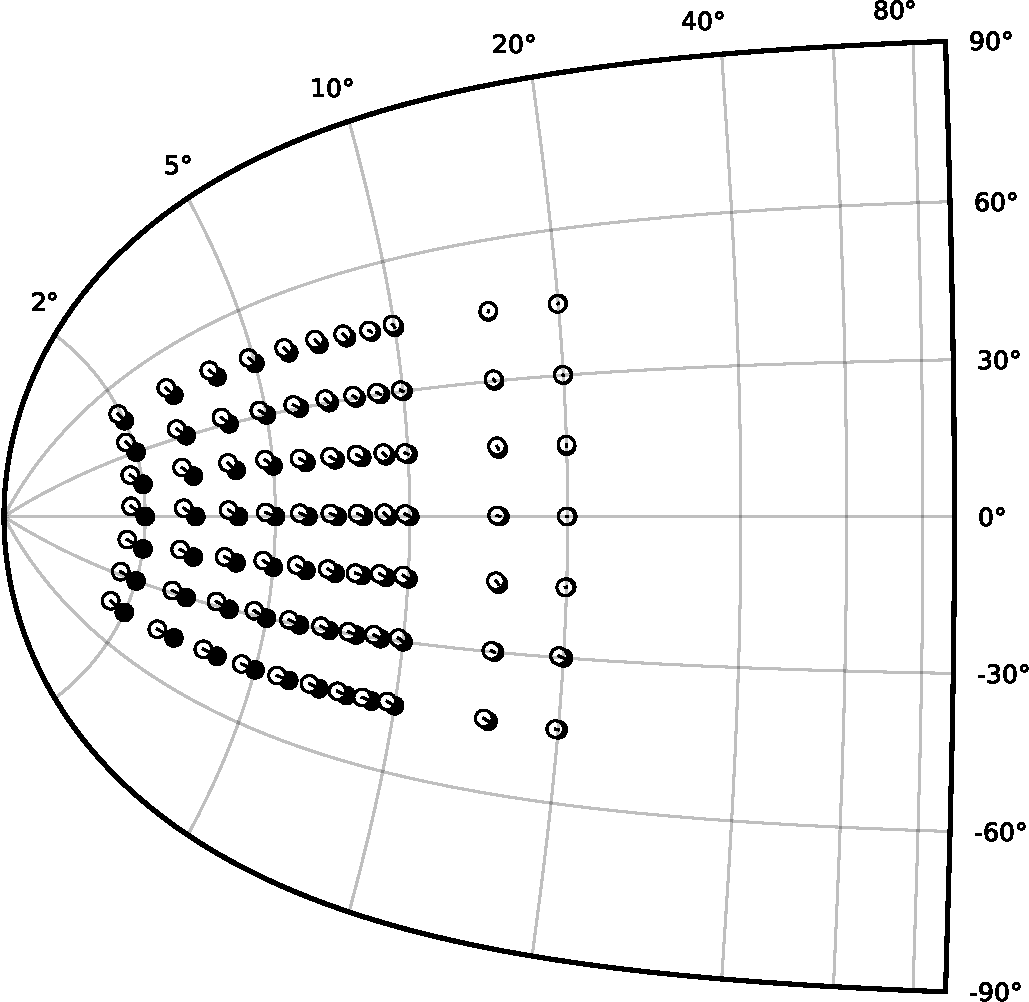
\includegraphics[width=0.4\textwidth]{figures/ch3_6_lesion-1} &
      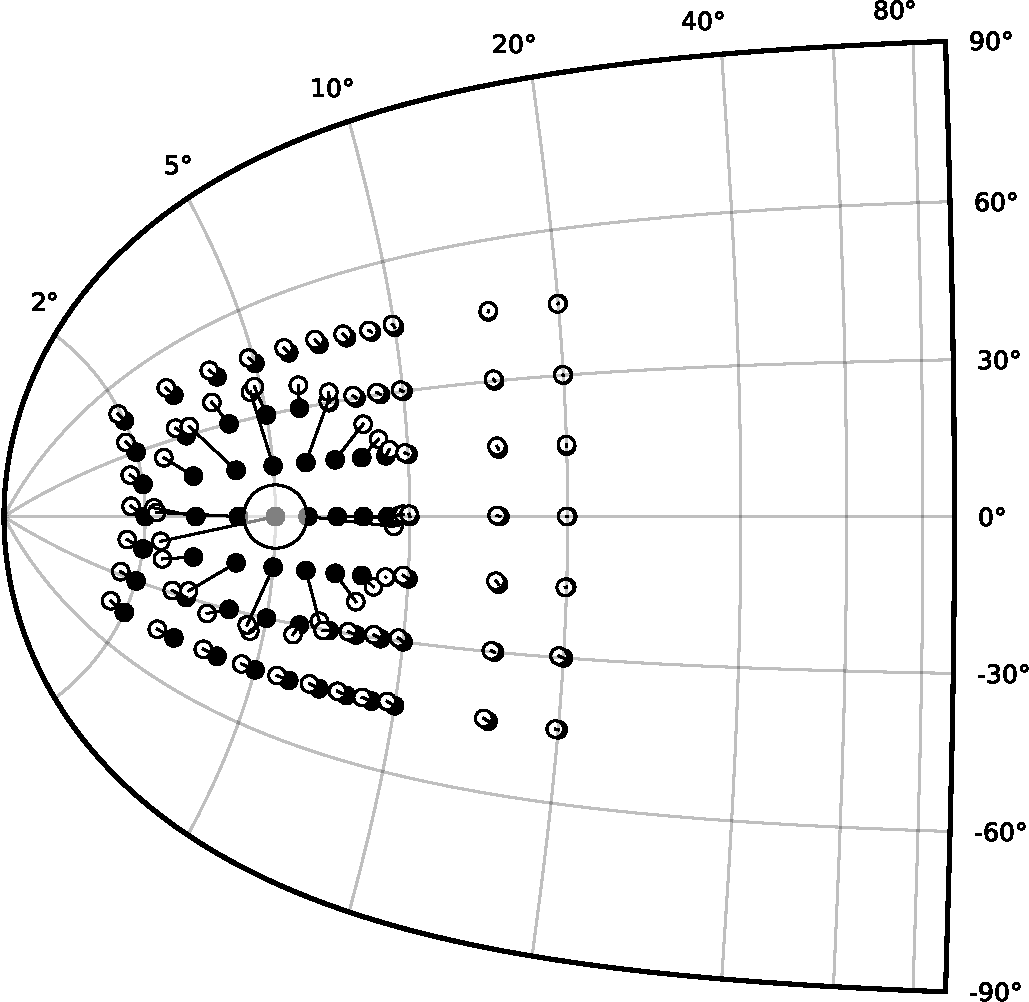
\includegraphics[width=0.4\textwidth]{figures/ch3_6_lesion-2} \\
      {\textsf {\textbf C}} &
      {\textsf {\textbf D}} \\     
      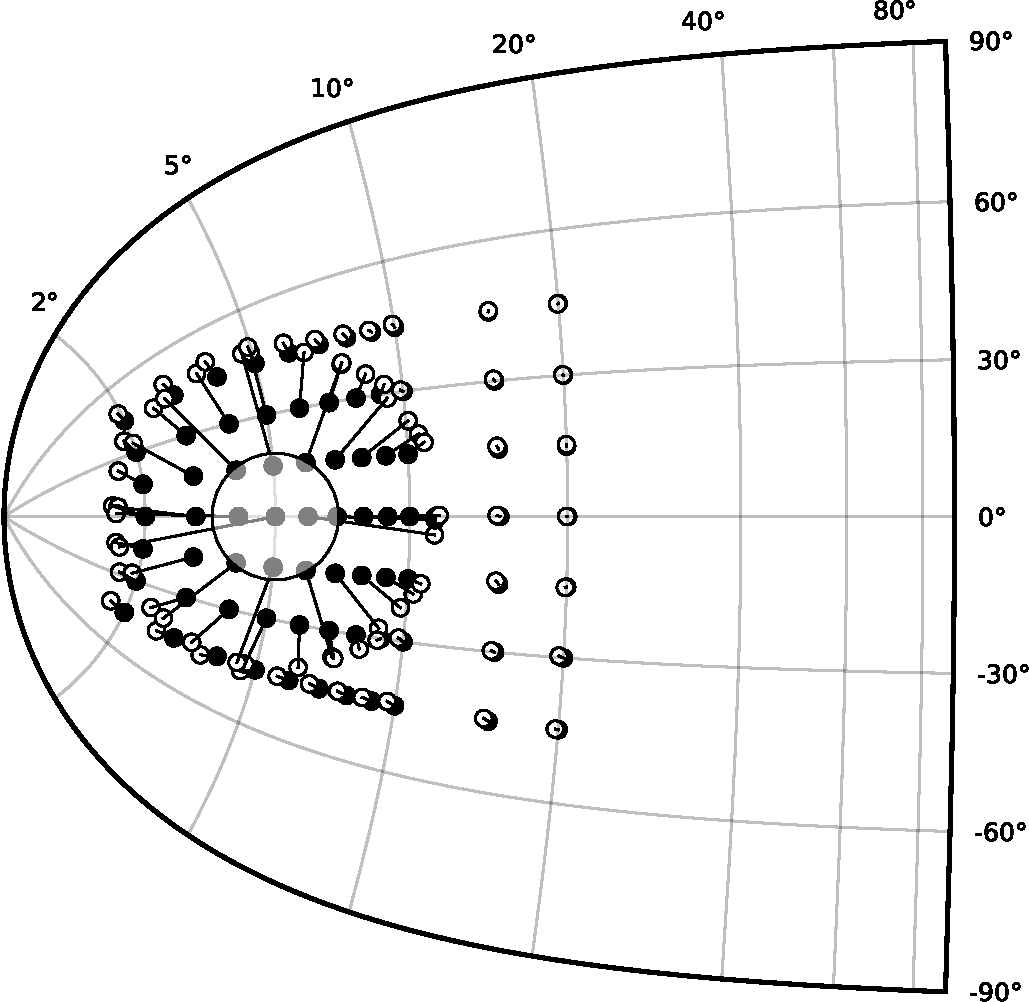
\includegraphics[width=0.4\textwidth]{figures/ch3_6_lesion-3} &
      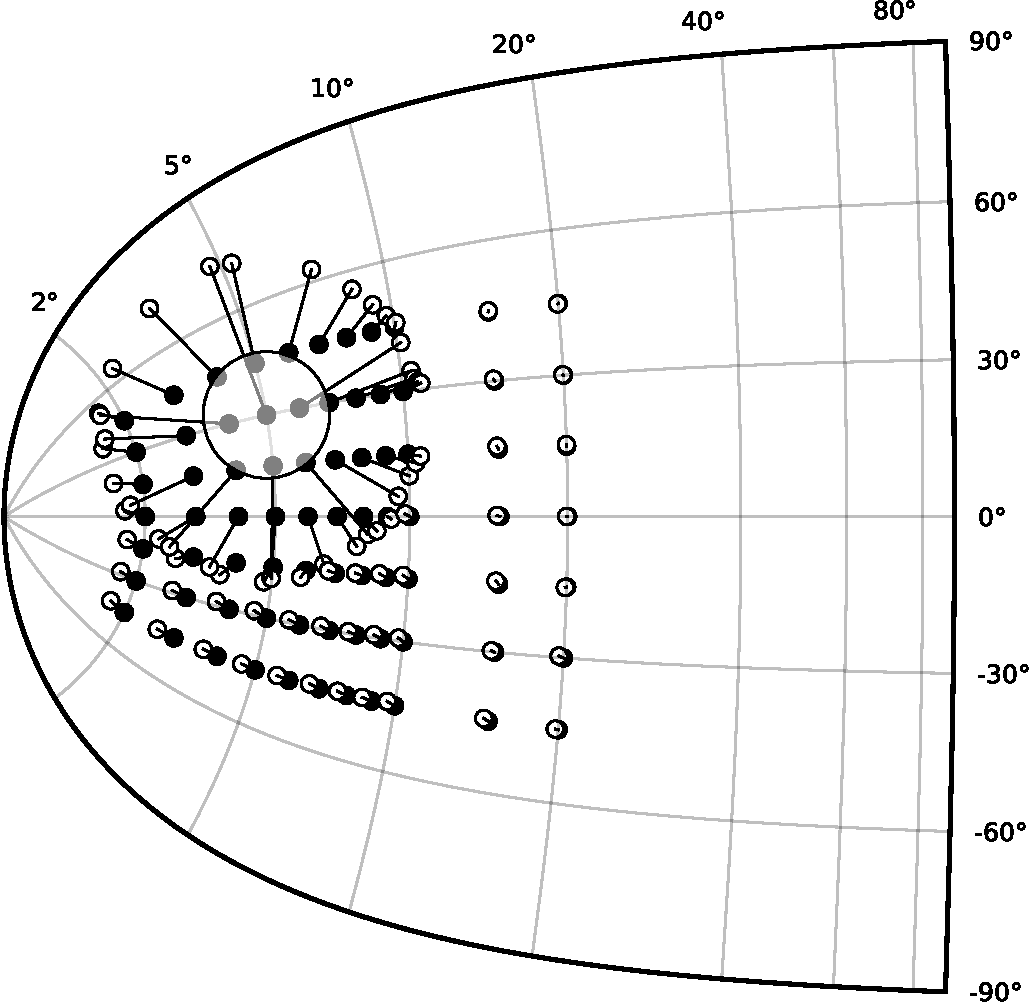
\includegraphics[width=0.4\textwidth]{figures/ch3_6_lesion-4} \\
    \end{tabular}
    \begin{tabular}[t]{cccc}  
      {\textsf {\textbf E}} &
      {\textsf {\textbf F}} &
      {\textsf {\textbf G}} &
      {\textsf {\textbf H}} \\
      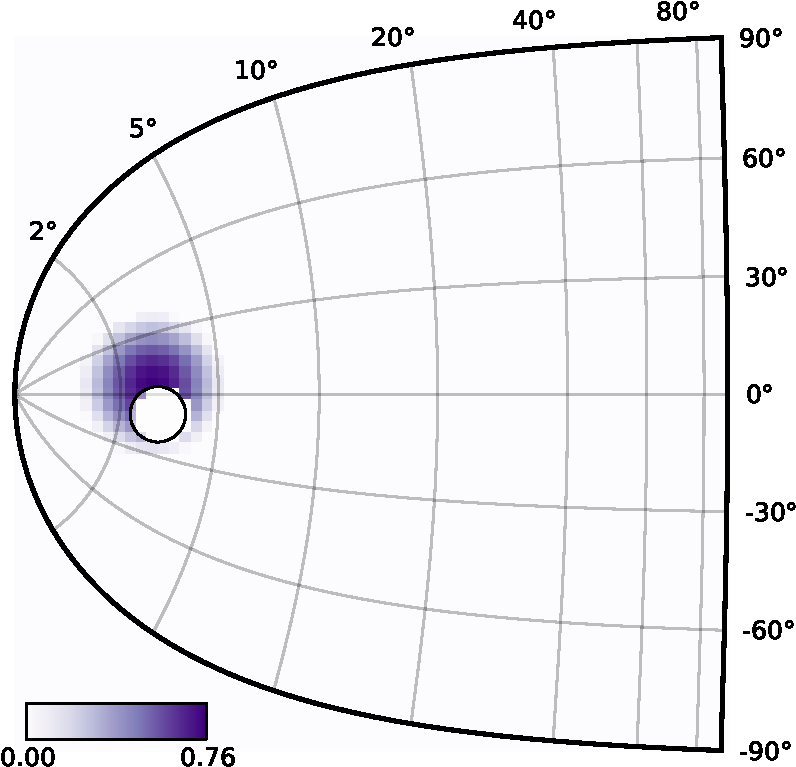
\includegraphics[width=0.23\textwidth]{figures/ch3_6_lesion-after-5} &
      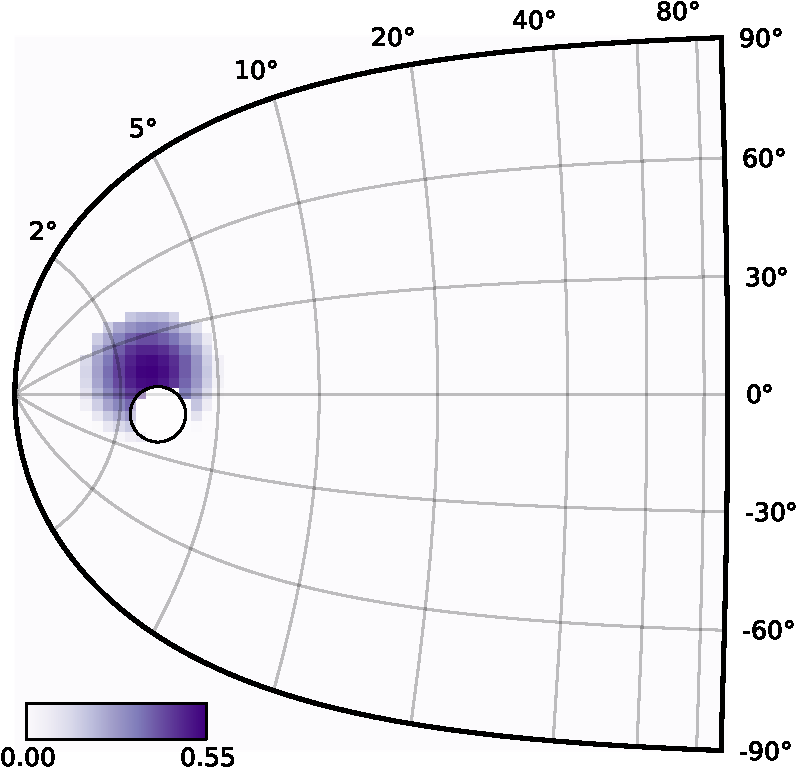
\includegraphics[width=0.23\textwidth]{figures/ch3_6_lesion-after-25} &
      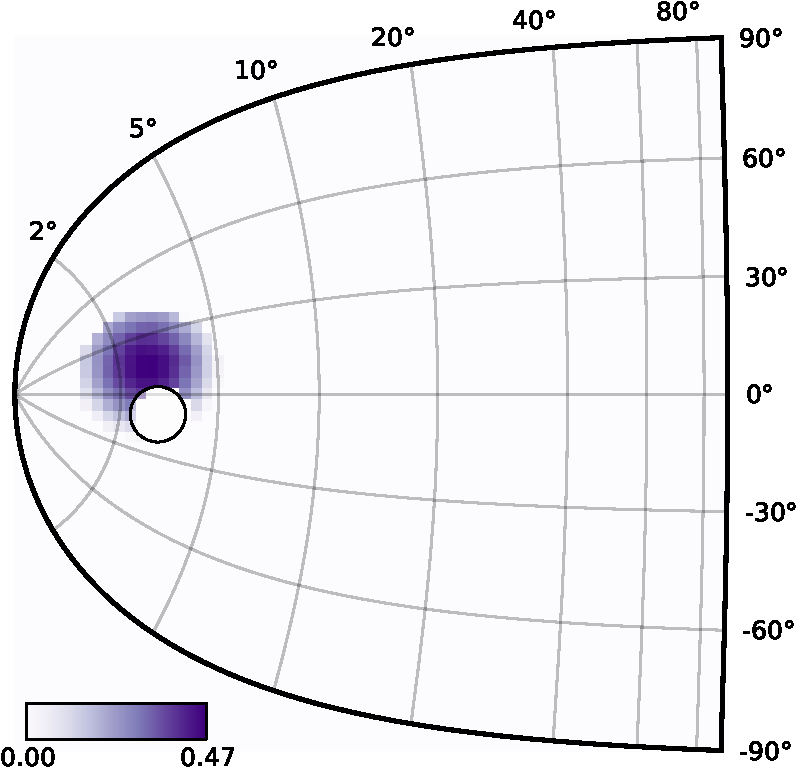
\includegraphics[width=0.23\textwidth]{figures/ch3_6_lesion-after-50} &
      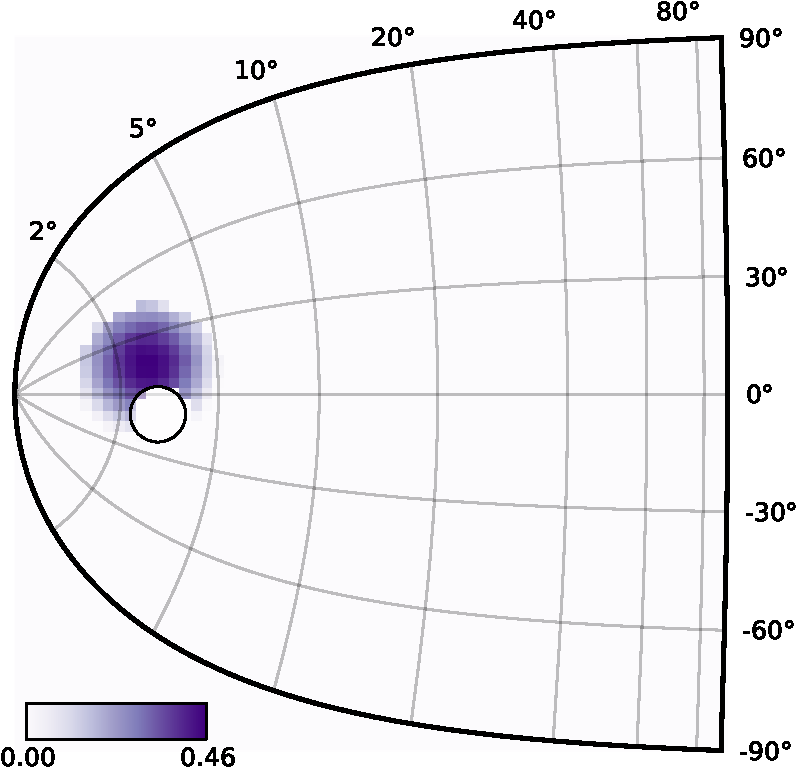
\includegraphics[width=0.23\textwidth]{figures/ch3_6_lesion-after-100}  \\
    \end{tabular}
  \end{center}

  \caption{Exactitude du décodage et effet des lésions sur l'activité colliculaire. L'exactitude du modèle a été examinée sur un ensemble de cibles à des emplacements différents présentés séquentiellement au modèle. Pour chaque cible, le centre de masse de l'activité colliculaire est décodé et représenté par un cercle (vide) alors que la position théorique est représentée par un cercle plein. A. Le modèle sans lésions. B. Une petite lésion circulaire à la position (5°, 0°). C. Une lésion de taille moyenne à la position (5°, 0°). D. Une lésion de taille moyenne à la position (5°, 30°). E.F.G.H. Effet de l'inactivation sur l'activation de la carte colliculaire à différents pas (respectivement 5ms, 25ms, 50ms et 100ms après l'apparition du stimulus). La population active se décale loin du site de la lésion. }
  \label{fig: accuracy}
\end{figure}


\subsection{Temps de r\'eponse}

Nous avons étudié l'effet de la taille, l'intensité et l'excentricité du stimulus rétinien sur la réponse colliculaire. La figure (fig \ref{fig: time}) montre l'évolution temporelle de l'activation maximale (fréquence de décharge) en fonction du temps pour plusieurs excentricités en fixant la taille et l'intensité aux valeurs standards (fig \ref{fig: time}-A), pour plusieurs tailles du stimulus en fixant l'excentricité à 5 et l'intensité à 1 (fig \ref{fig: time}-E) et pour plusieurs intensités en fixant la taille à 1 et l'excentricité à 5 (fig \ref{fig: time}-C).\\

Le temps de latence d'une saccade est défini comme le temps écoulé entre la présentation d'une cible et le déclenchement des saccades. C'est par rapport à cette notion qu'on définit donc le temps de réponse de notre modèle. Nous avons choisi un seuil arbitraire de fréquence de décharge maximale à partir duquel on suppose qu'une saccade peut être déclenchée (400HZ).  Mais si on revient aux courbes d'accord, les neurones les plus excentrés ne sont pas capables d'atteindre des seuils d'activation élevés, donc le seuil qu'on avait défini ne s'applique qu'aux stimuli qui se projettent sur la zone rostrale. Un autre critère pourrait être utilisé, à savoir le temps nécessaire pour que l'activation sur la carte colliculaire atteigne un état plus stable\footnote{On suppose que la bulle d'activité est stabilisée quand la variation de la somme des activités entre t et t+1 devient inférieure à une petite valeur $epsilon$}. En examinant les courbes A,C et E, on peut prédire qu'on va obtenir des effets contradictoires avec ceux obtenus par le critère du seuil (moins l'état final est élévé, moins la croissance de la courbe est rapide et plus le temps de stabilisation est court).\\

Les courbes de variations de temps de réponse en fonction des 3 critères: excentricité, taille et intensité sont tracées respectivement dans les figures (fig \ref{fig: time}-B),(fig \ref{fig: time}-D) et (fig \ref{fig: time}-F). Les points de saturation à 500 ms correspondent aux valeurs de variables qui n'ont pas permis d'atteindre le seuil d'activation (choix numérique). En ce qui concerne l'influence de la taille (fig \ref{fig: time}-E et \ref{fig: time}-F ) et l'intensité du stimulus (fig \ref{fig: time}-C et \ref{fig: time}-D), le temps de réponse décroît avec l'augmentation de ces deux paramètres. En effet, plus l'activation initiale est importante, plus l'augmentation des activités individuelles est rapide (excitations mutuelles). \\

Si on varie l'excentricité, on a l'effet inverse. En effet, moins le stimulus est excentré, plus l'activation initiale est importante à cause de la magnification et par la suite plus l'atteinte du seuil de déclenchement est rapide.\\ 

Nous gardons donc le premier critère, en supposant en plus qu'une correction supplémentaire pourrait s'ajouter à la sortie du colliculus permettant d'amplifier les activations caudales pour donner aux générateurs de motifs moteurs une activation stéréotypée (par exemple, ajouter une fonction qui dépend exponentiellement de la position horizontale dans la carte).






\begin{figure}
  \begin{center}
    \begin{tabular}[t]{cc}
     {\textsf {\textbf A}} &
      {\textsf {\textbf B}} \\
      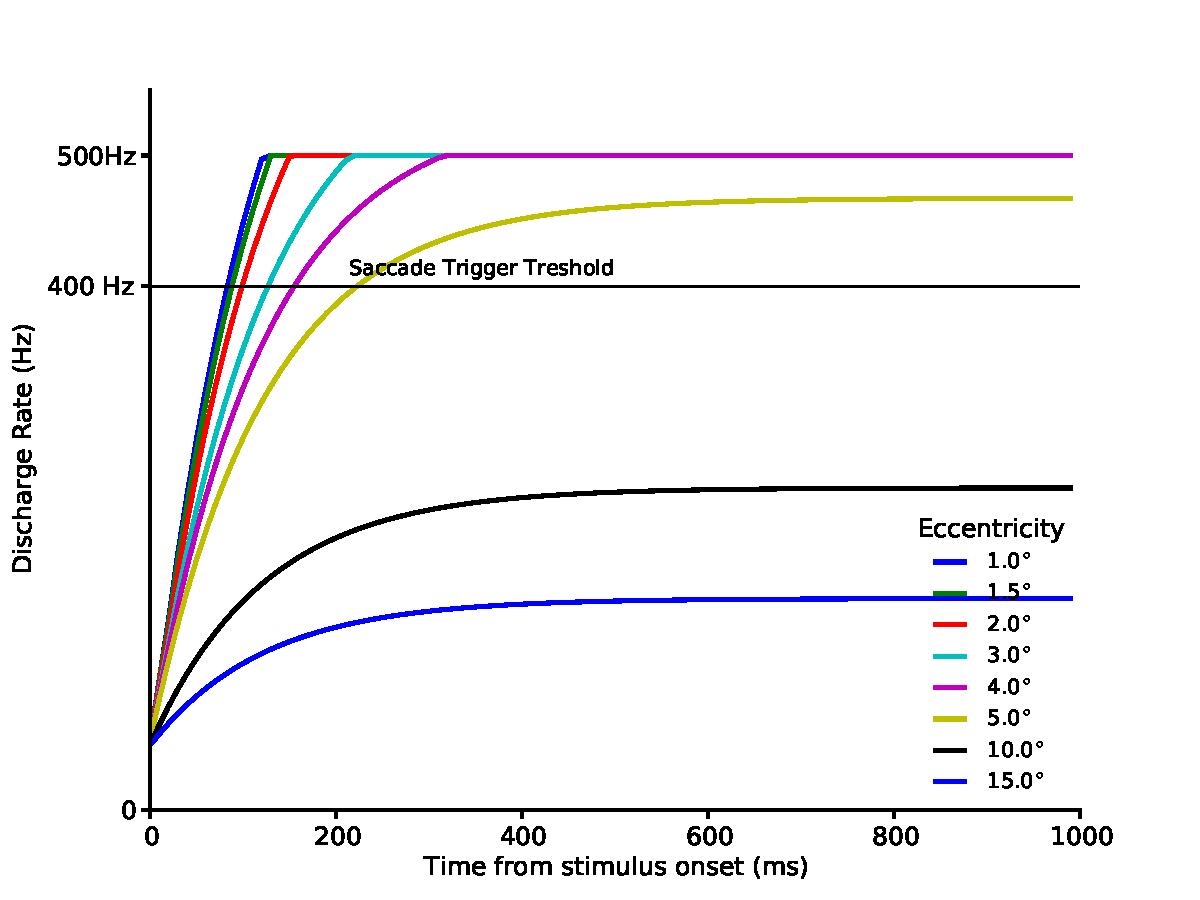
\includegraphics[width=0.5\textwidth]{figures/ch3_7_RT-eccentricity-A} &
      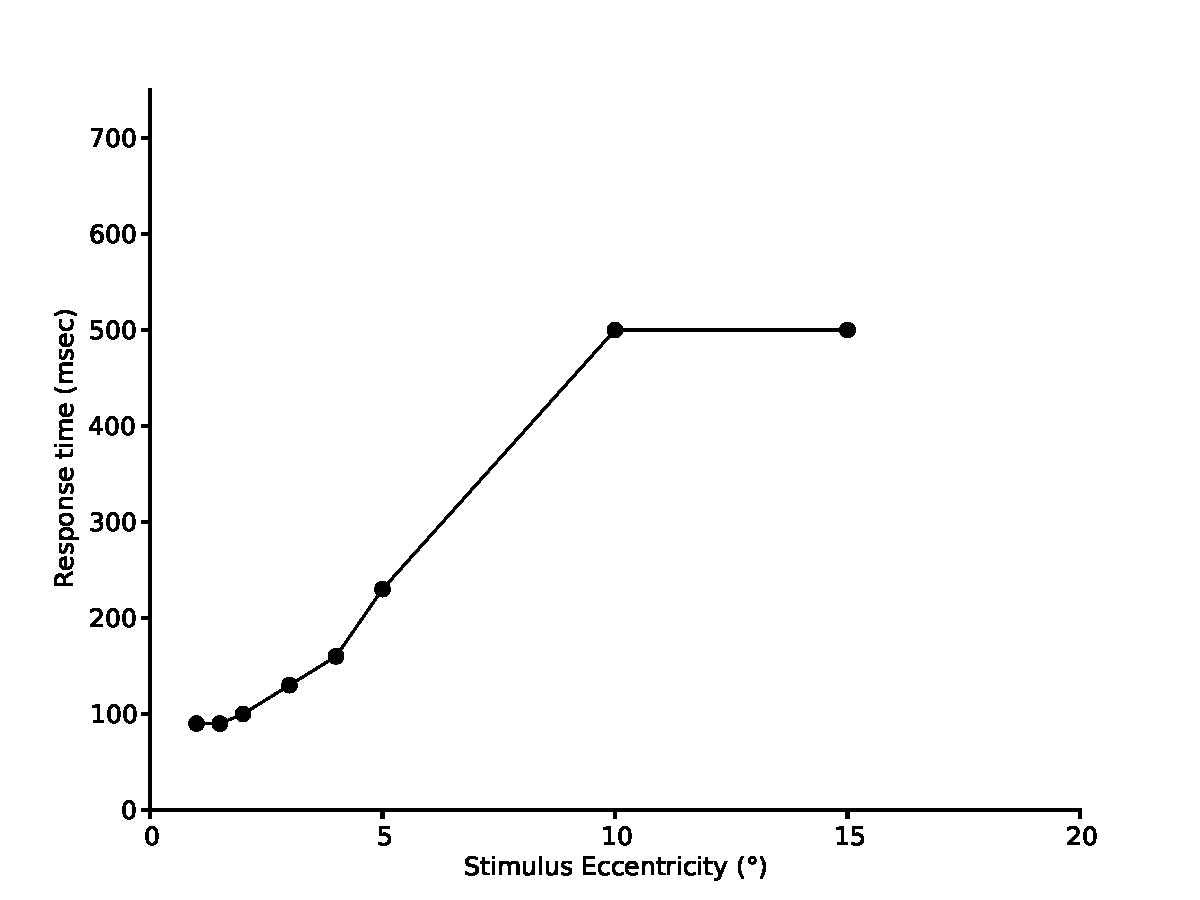
\includegraphics[width=0.5\textwidth]{figures/ch3_7_RT-eccentricity-B} \\
      {\textsf {\textbf C}} &
      {\textsf {\textbf D}} \\     
      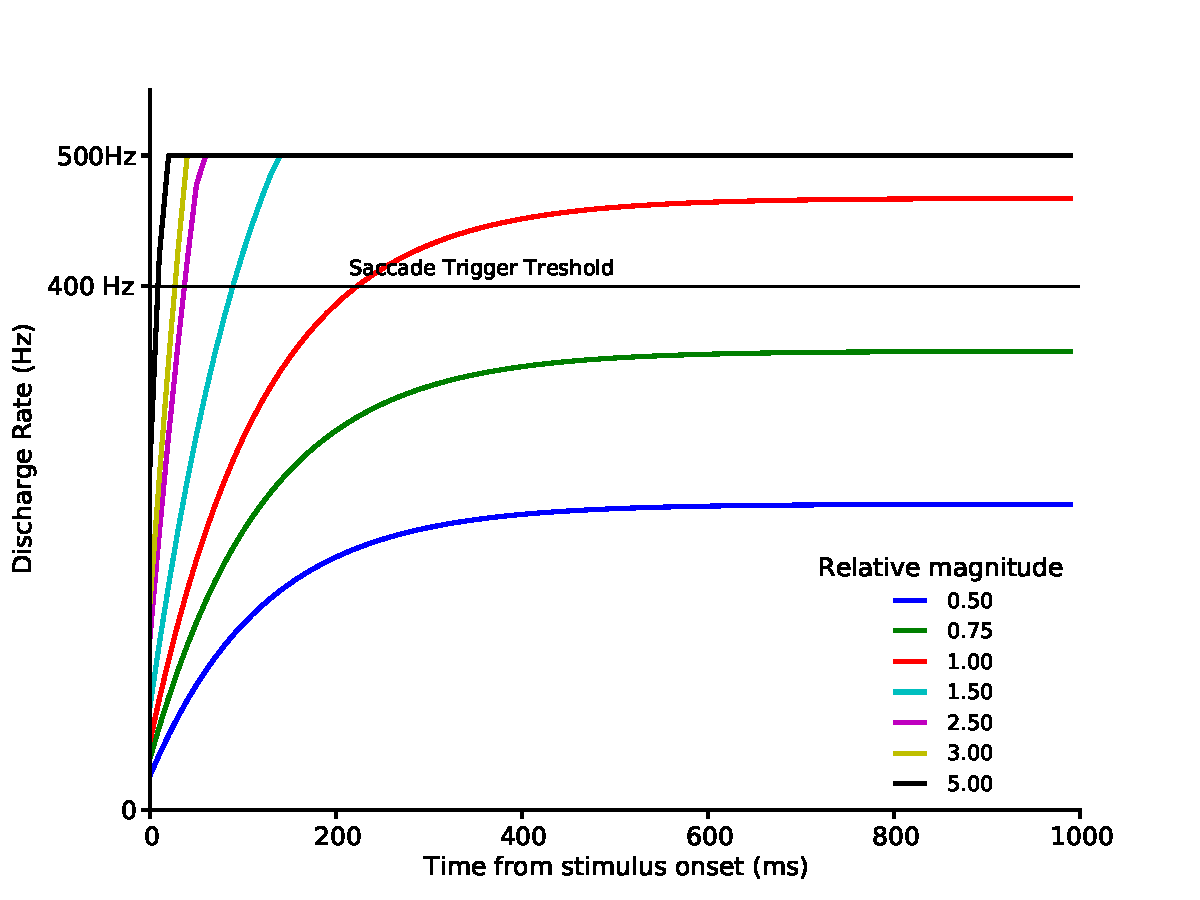
\includegraphics[width=0.5\textwidth]{figures/ch3_7_RT-size-A} &
      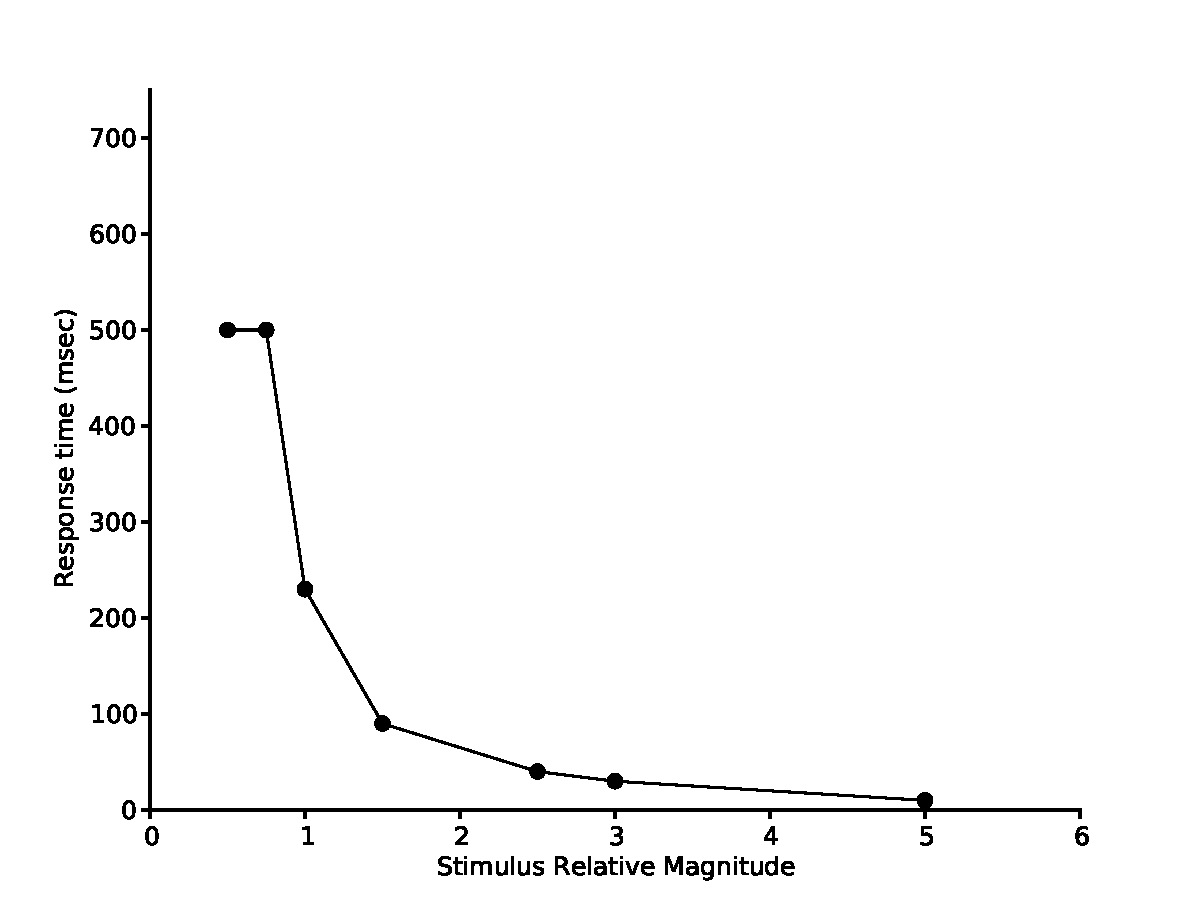
\includegraphics[width=0.5\textwidth]{figures/ch3_7_RT-size-B} \\
      {\textsf {\textbf E}} &
      {\textsf {\textbf F}} \\     
      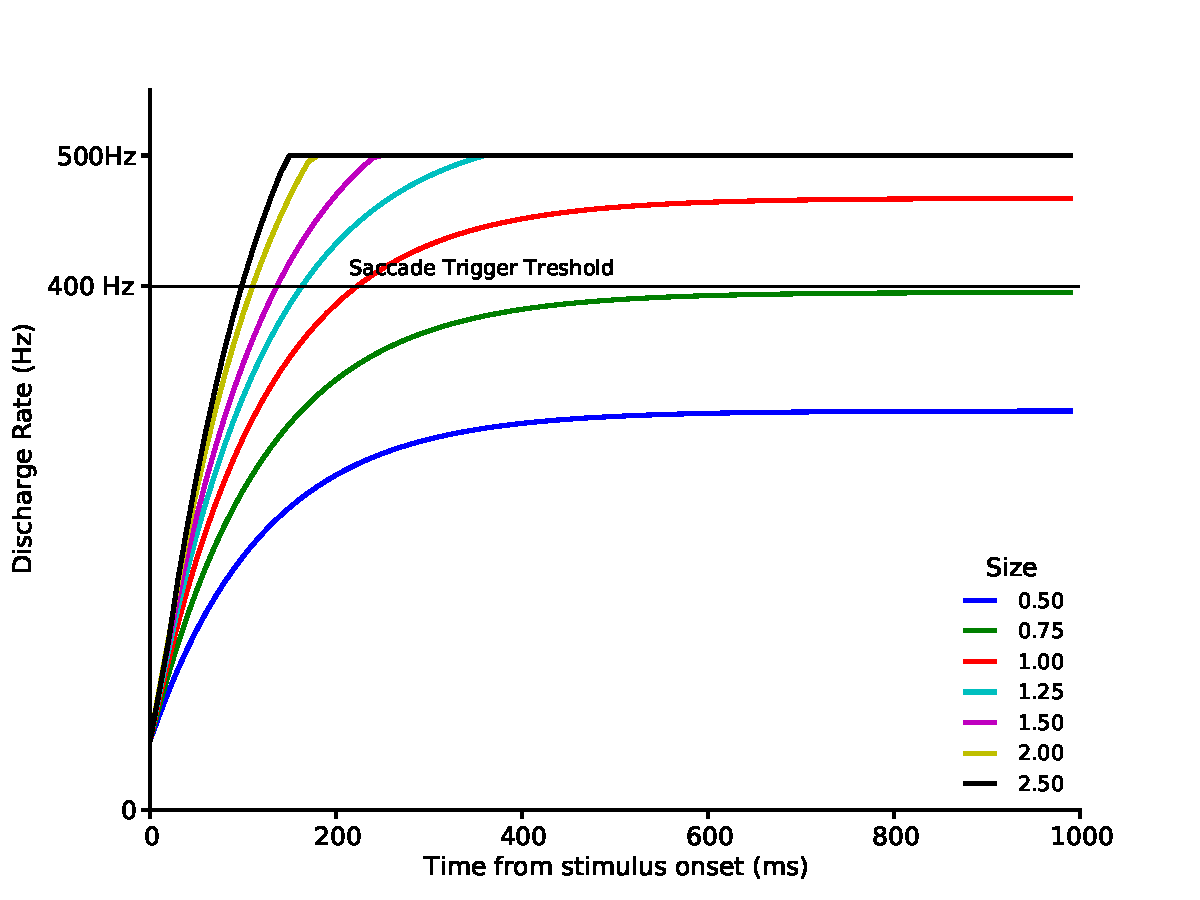
\includegraphics[width=0.5\textwidth]{figures/ch3_7_RT-magnitude-A} &
      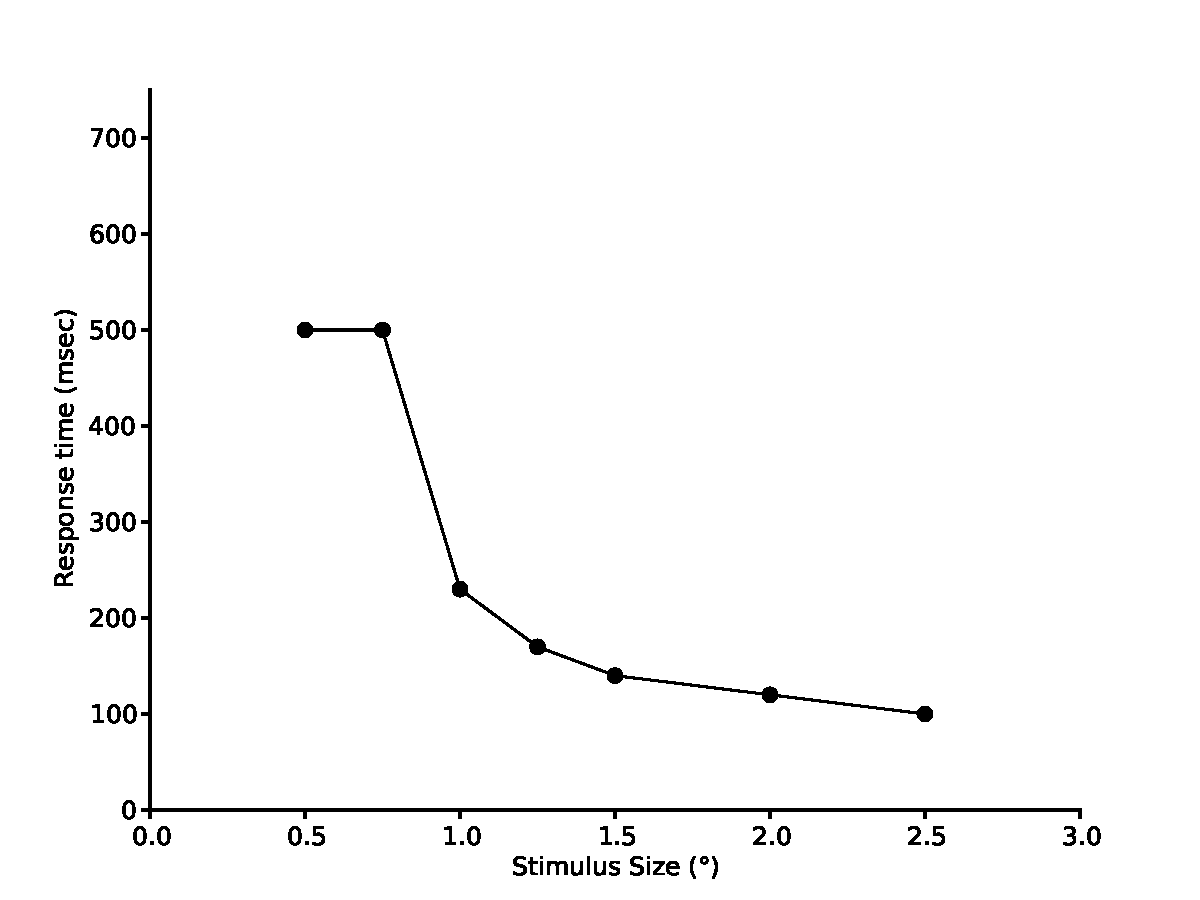
\includegraphics[width=0.5\textwidth]{figures/ch3_7_RT-magnitude-B} \\
    \end{tabular}

  \end{center}

  \caption{Influence de l'excentricité, de la taille et de l'intensité du stimulus sur le temps de réponse. A et B: Le stimulus a été présenté à des excentricités différentes et l'activation a été enregistrée jusqu'à ce qu'elle atteigne la valeur maximale. Le temps de réponse est mesuré quand l'activation atteint le seuil de déclenchement d'une saccade. C et D: Le temps de réponse a été mesuré pour différentes intensités de stimuli (l'intensité de référence vaut 1). E et F: Le temps de réponse a été mesuré pour des stimuli de différentes tailles (la taille de référence vaut 1/90).
  }
  \label{fig: time}
\end{figure}


\subsection{Interactions spatiales entre deux stimuli à excentricités différentes} 


Quand deux (ou plusieurs) stimuli sont présentés sur la rétine, ils activent initialement plusieurs emplacements sur la carte du \gls{sc}. Cependant, après que la carte atteint un état d'activation stable, une seule sous-population d'unités neurales préalablement activées reste active.\\

\begin{figure}
  \begin{center}
      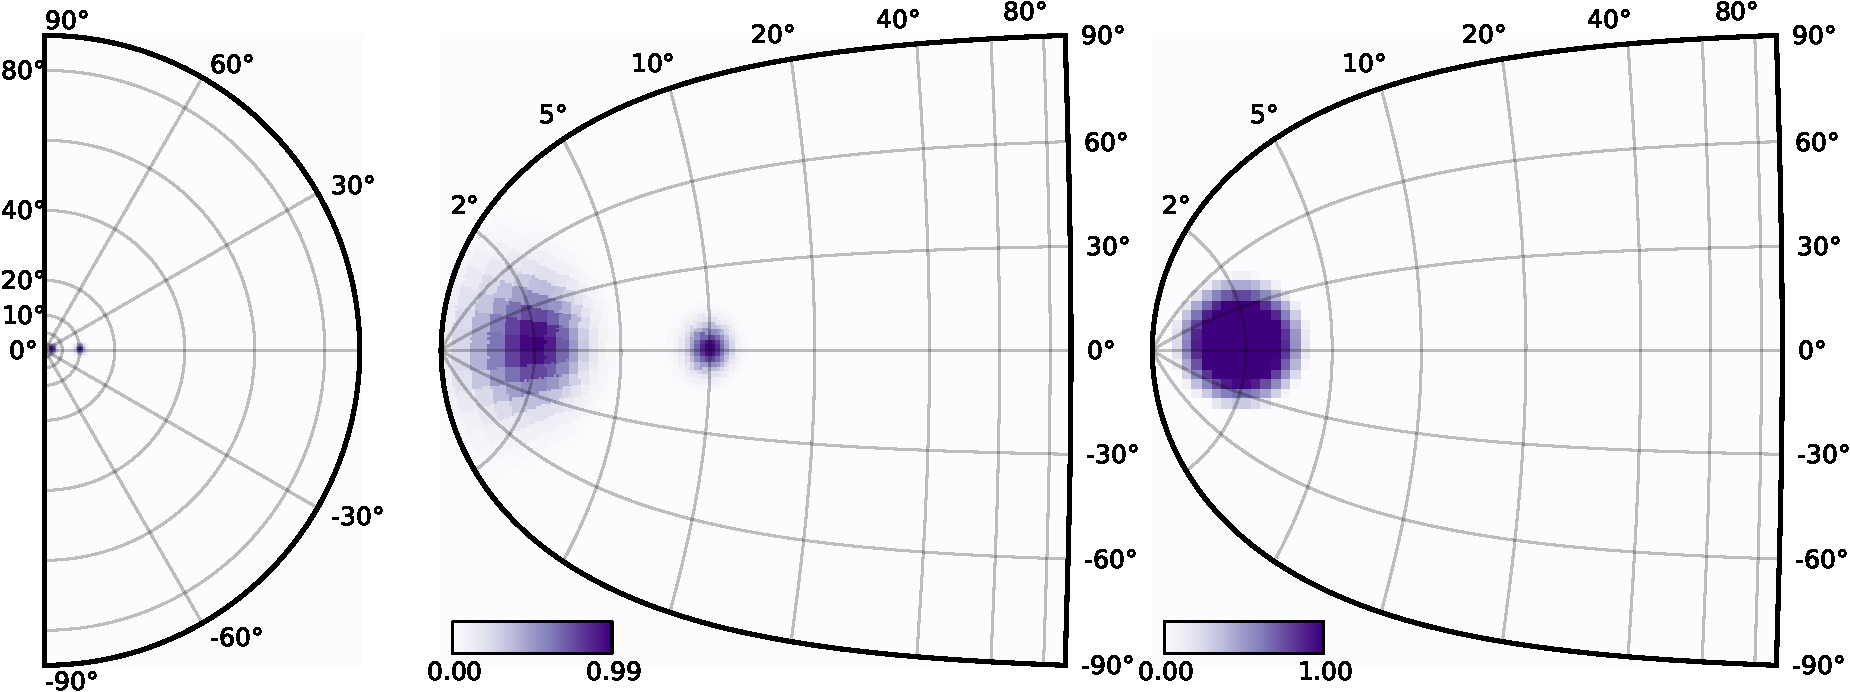
\includegraphics[width=\textwidth]{figures/ch3_8_stimulus-2} 
  \end{center}
  \caption{Interaction spatiale entre deux stimuli identiques à deux positions à même amplitude (0°) et à excentricités différentes (3° et 10°). Le stimulus à 3° active initialement une population plus importante et gagne au final la compétition.
  }
  \label{fig: space}
\end{figure}

 La figure (fig \ref{fig: space}) montre la réponse de notre modèle à la présentation de deux stimuli identiques (même taille, intensité et forme) situés à différents emplacements (3 et 10°). La figure du milieu correspondant à la carte intermédiaire (l'entrée colliculaire suite à la déformation logarithmique) montre que la population activée par le stimulus rostral (3°) est initialement plus grande que la population activée par le stimulus le plus caudal (10°). A la fin de la simulation, figure à droite, l'activité dans le \gls{sc} atteint un état stable et la population active résultante est située dans la position la moins excentré. Le stimulus le plus fovéal a été choisi alors que l'autre a été inhibé sous l'effet de la connectivité latérale.

\subsection{Interactions spatiales entre deux stimuli à excentricités identiques}

Le comportement de sélection a été souvent étudié lorsque deux stimulus sont présentés simultanément avec des excentricités identiques et des amplitudes opposés. La figure \ref{fig: distractor} montre que pour une distance angulaire inférieur à 50° entre les deux cibles, la sous-population résultante des unités neurales actives dans le \gls{sc} est située dans une position intermédiaire entre les deux sites codant l'emplacement de chaque cible, tandis que pour une distance supérieure à 50°, la sous-population active résultante est située à l'un des deux emplacements. Cette sélection est faite quand on ajoute un bruit blanc à l'activité. C'est surtout le phénomène qui est intéressant, la valeur 50° résulte des paramètres choisis et pourrait donc être ajustée.\\

\begin{figure}
  \begin{center}
    \begin{tabular}[t]{c}
     {\textsf {\textbf A}}  \\
      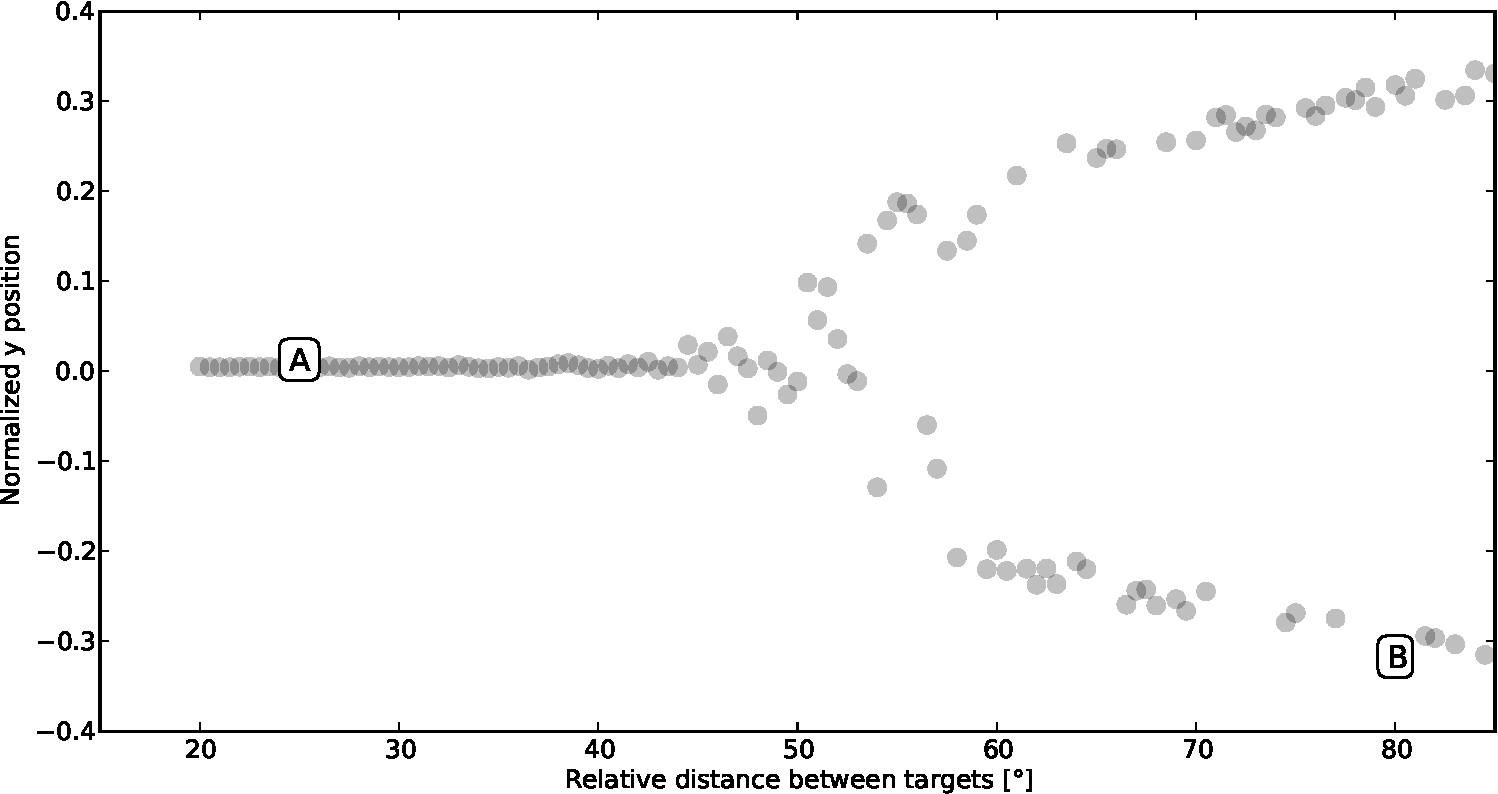
\includegraphics[height=6cm]{figures/ch3_9_global-effect}  \\
    \end{tabular}
    \begin{tabular}[t]{ccc}
      {\textsf {\textbf B}} &
      {\textsf {\textbf C}} &
      {\textsf {\textbf D}} \\     
      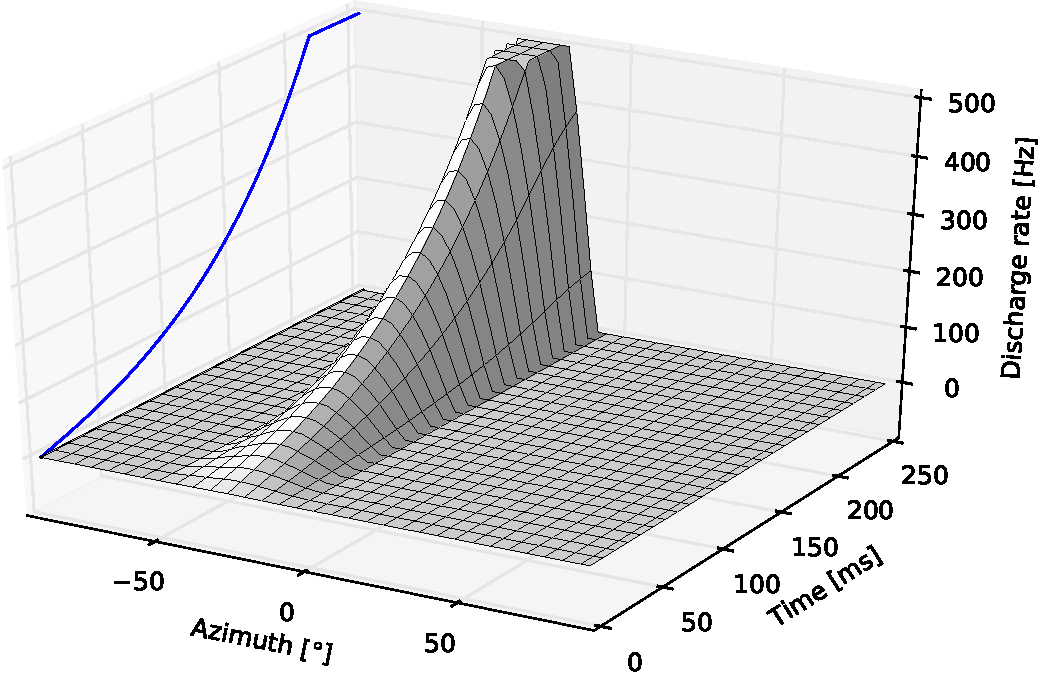
\includegraphics[width=0.33\textwidth, height=6cm]{figures/ch3_9_distractor-effect-1} &
      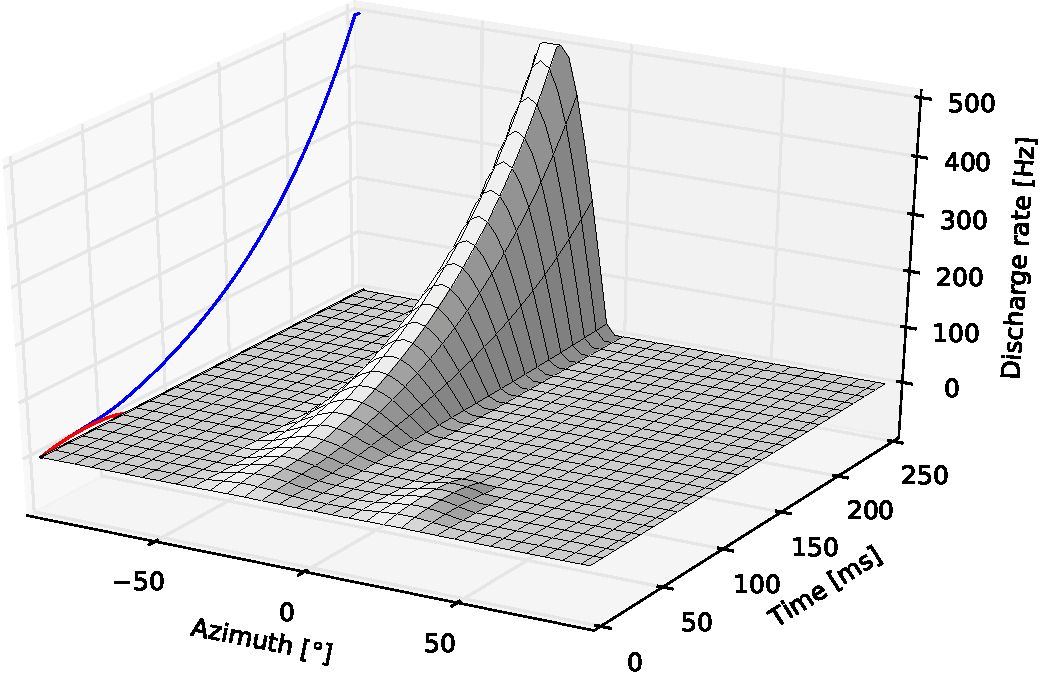
\includegraphics[width=0.33\textwidth, height=6cm]{figures/ch3_9_distractor-effect-2} &
      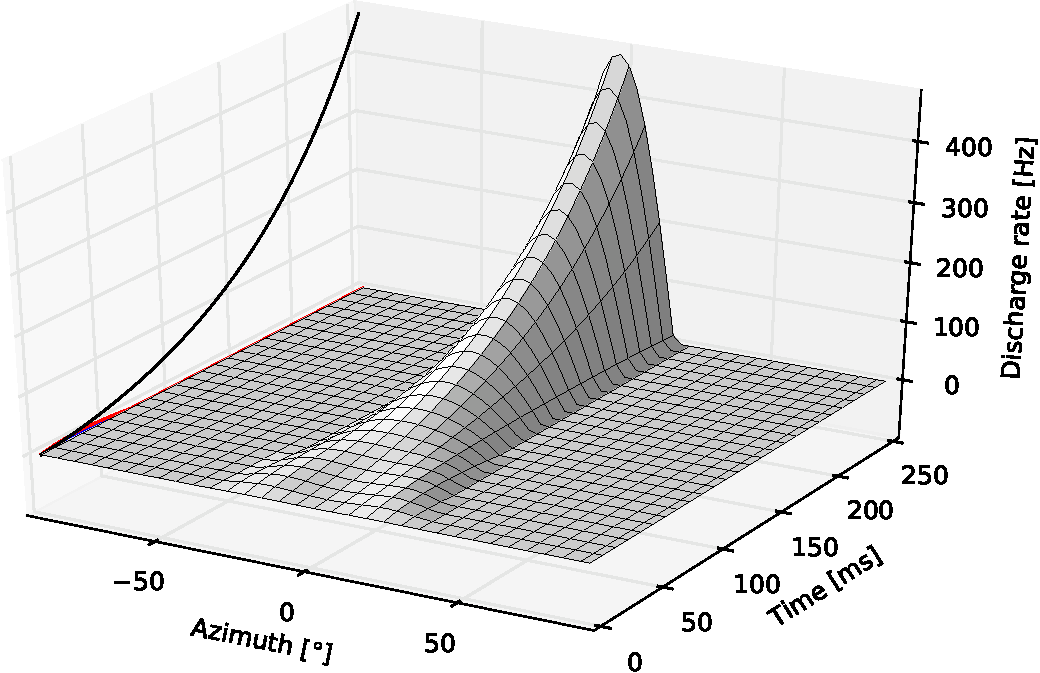
\includegraphics[width=0.33\textwidth, height=6cm]{figures/ch3_9_distractor-effect-3} \\
    \end{tabular}
    \begin{tabular}[t]{cc}
      {\textsf {\textbf E}} &
      {\textsf {\textbf F}} \\     
      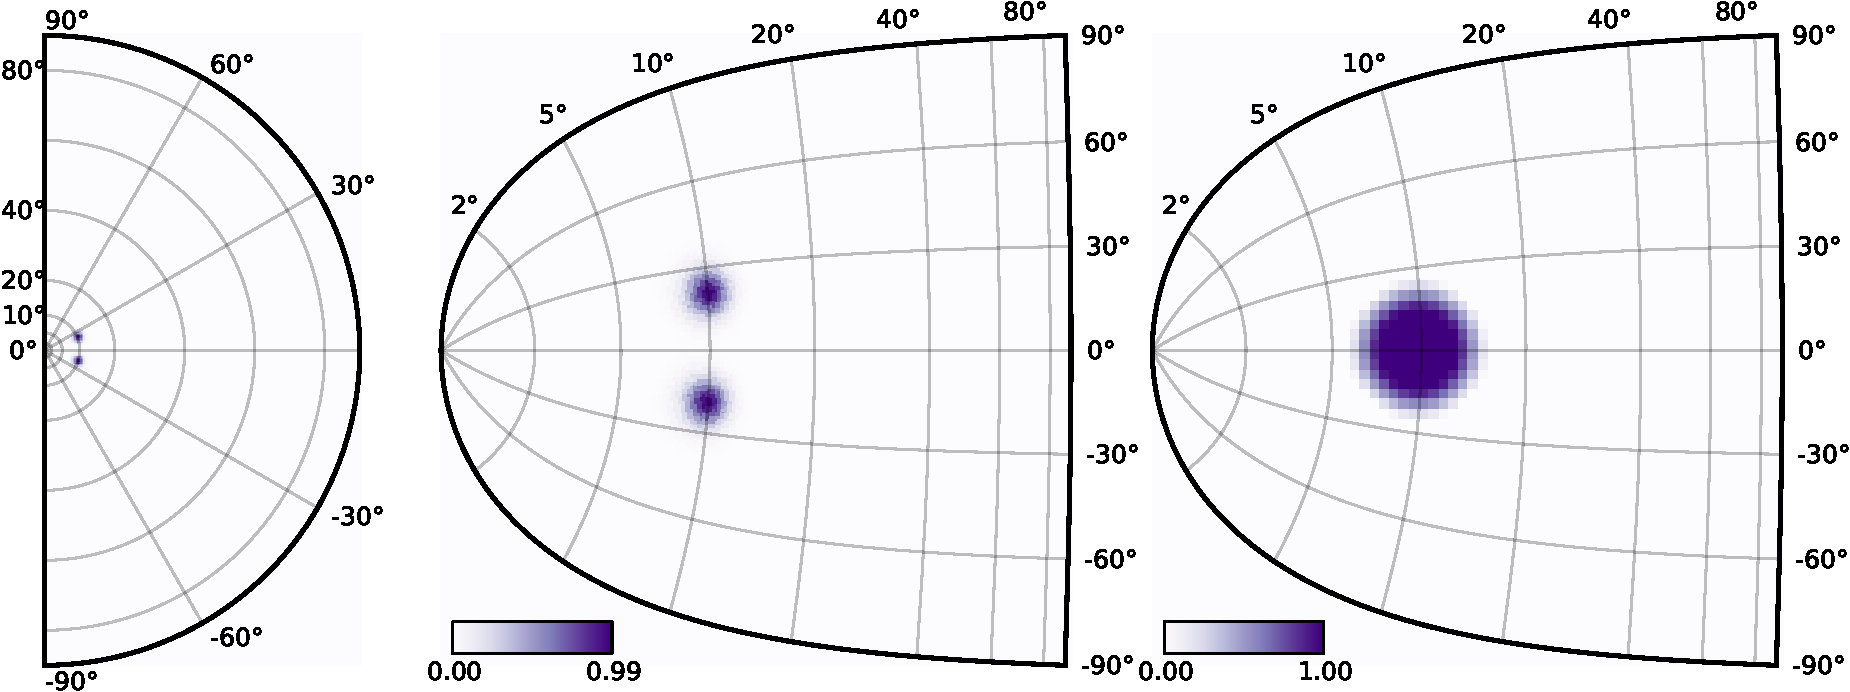
\includegraphics[width=0.5\textwidth]{figures/ch3_9_stimulus-3} &
      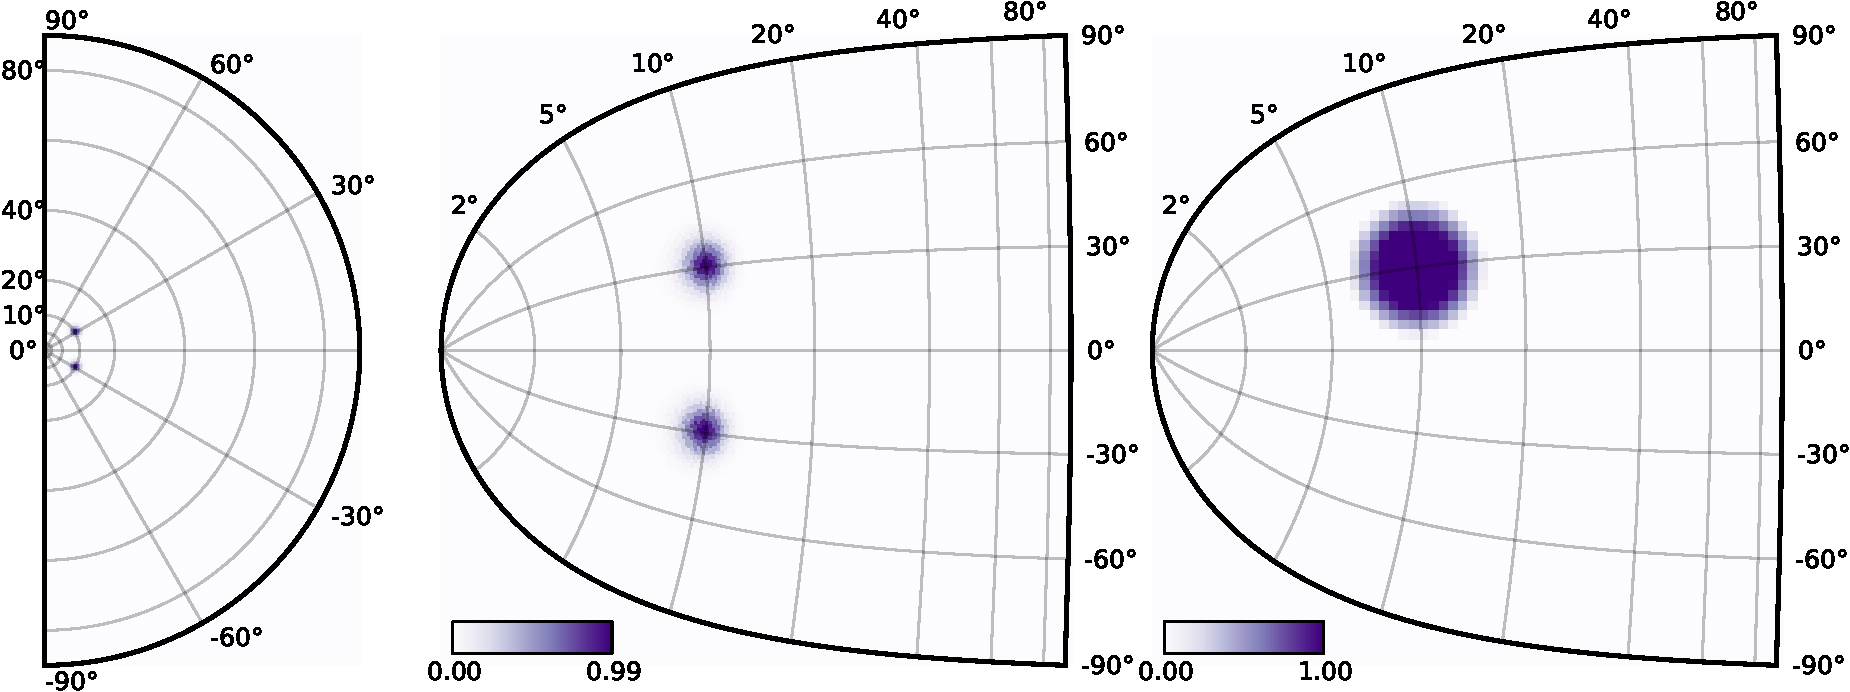
\includegraphics[width=0.5\textwidth]{figures/ch3_9_stimulus-4} \\
    \end{tabular}

  \end{center}

  \caption{Sélection entre deux cibles. A. La position de la cible décodée dans le \protect\gls{sc} après 500ms de simulation. Quand la distance relative entre les deux stimulus est supérieur à 50°, un des deux stimuli est sélectionné. B. L'évolution temporelle de l'activité de la carte du \protect\gls{sc} quand un seul stimuli est présenté. C. L'évolution temporelle de l'activité de la carte du \protect\gls{sc} quand un stimulus est sélectionné. D. L'évolution temporelle de l'activité sur la carte du \protect\gls{sc} montre la fusion des activités au niveau du centre de masse des positions des deux stimuli (pas de sélection). E. L'activation finale du \protect\gls{sc} quand la saccade encodée correspond au centre de masse des deux stimuli (distance relative entre les deux stimuli inférieure à 50°). F. L'activation finale du \protect\gls{sc} quand la saccade encodée correspond à la position de l'un des deux stimuli (distance relative entre les deux stimuli égale à 60°).
  }
  \label{fig: distractor}
\end{figure}


\subsection{Effet de latence}

On peut également examiner l'effet de latence (ralentissement) lors du processus de sélection jusqu'à la stabilisation de l'activité dans la carte colliculaire. Prenons le cas particulier illustré par la figure (fig \ref{fig: distractor}-B et C), quand les deux sous-populations actives ont initialement la même taille (parce que les deux cibles identiques sont à la même excentricité), mais correspondent à des directions opposées. L'évolution de l'activité du \gls{sc} au cours de temps est examinée pour un stimulus simple et comparée à l'activité du colliculus quand ce stimulus est accompagné par un autre stimulus identique à un emplacement symétrique (voir les lignes de projections des courbes (fig \ref{fig: distractor}-B, C et D) en bleu la projection de l'évolution de l'activation maximale causée par le premier stimulus, en rouge celle causée par le deuxième stimulus et en noir l'activation maximale moyenne).

\subsection{Effet de l'inactivation de la carte colliculaire}

Nous avons examiné les effets de l'inactivation d'une petite partie de la carte du \gls{sc}. Dans la figure (fig \ref{fig: accuracy}-B), l'inactivation est imposée sur un site codant une cible située à (5°, 0°). Ensuite, nous avons étudié la réponse du modèle à des stimuli situés à différentes positions. Nous avons constaté que l'activité du \gls{sc} évoquée par les stimuli moins excentrés (4°, 20°) a été décalée vers la partie rostrale du \gls{sc} (correspondant à la projection de la partie fovéale) tandis que l'activité évoquée par une cible plus excentré (9°, - 20°) a été décalée vers l'extrémité caudale (en périphérie). En effet, à cause de l'inactivation, la symétrie de la population, qui est normalement activée pour ces localisations, est changée. La symétrie de l'organisation gaussienne de la connectivité inhibitrice est aussi altérée. La symétrie est rétablie par un décalage de l'activité du \gls{sc} loin du site de la lésion (fig \ref{fig: accuracy}, E, F, G et H). Par contre, un stimulus situé à (5°, 0°) active une population concentrée sur le site inactivé. Enfin, dans la figure, (fig \ref{fig: accuracy}-C), nous montrons l'influence d'une plus grande inactivation utilisant le même stimulus. Certaines des saccades qui n'ont pas été affectées par une petite lésion deviennent inexactes. 

\subsection{Traitement d'images naturelles}

Nous avons également testé le modèle en utilisant des images naturelles issues d'une caméra couleur (CCD). Aucun traitement n'a été réalisé sur l'image, sauf sa transformation en niveaux de gris. La figure (fig. \ref {fig: colliculus}) présente un exemple où une partie d'un clavier d'un ordinateur a été photographiée et introduite au modèle. Cela permet d'illustrer la principale caractéristique du modèle proposé. Si l'on regarde de près la rétine représentant la moitié du clavier (la partie supérieure gauche de la figure), on peut voir que plusieurs lettres ({\tt O, P, L, M} peuvent attirer l'attention et par la suite évoquer une saccade oculaire. Toutefois, la projection rétinotopique sur la carte intermédiaire (V1) du modèle réduit tout naturellement cet ensemble de lettres à {\tt O} et {\tt l}.\\

\begin{figure*}
  \centering
    \includegraphics[width=1.0\textwidth]{figures/ch3_10_colliculus-1}\\
    \includegraphics[width=1.0\textwidth]{figures/ch3_10_colliculus-2}
  \caption{Une image (en couleurs) d'un clavier d'un ordinateur a été prise par une caméra couleur (de résolution $1024 \times 1280$) et transformé en une image en niveaux de gris (normalisés). \textbf{Les figures du haut.} La moitié de droite de l'image a été présentée dans la demi rétine comme entrée de notre modèle. La figure du milieu représente la projection selon l'équation \ref{eq: mapping}. La compétition dans la carte colliculaire fait gagner l'endroit le plus saillant (la lettre {\tt O}) \textbf{Les figures du bas.} Après la saccade, l'image rétinienne est centrée sur la lettre {\tt O}. L'activité colliculaire se concentre alors sur une partie de cette lettre qui semble être l'endroit le plus saillat d'o\`u la position rostrale de l'activation finale de la carte du colliculus.}
  \label{fig: colliculus}
\end{figure*}


Le modèle du \gls{sc} est donc confronté à un choix entre ces deux endroits et la théorie du champ dynamique, comme il a été introduit dans la section précédente, garantit qu'un seul emplacement reste après la compétition. Toutefois, il est difficile de préciser les conditions exactes qui font que le modèle va se concentrer sur la lettre {\tt O} au lieu de la lettre {\tt L} dans l'exemple donné. La forme de la représentation spatiale de la lettre {\tt O} est certainement à prendre en compte.

\section{Discussion}

\subsection{S\'election d'une seule population et stéréotypie des unités neurales actives}

Nous avons constaté que l'état de la carte colliculaire suite à la présentation d'un stimulus visuel se stabilise sur une seule sous-population stéréotypée. Ce résultat est compatible avec les résultats rapportés dans \cite{Anderson:1998}. \cite{Gandhi:2011} ont également évoqué ce phénomène et ont rapporté que la taille de la sous-population des neurones actifs couvre 28\% de la carte juste avant le début de la saccade. Dans l'étude théorique des \glspl{dnf} \cite{Amari:1977}, les auteurs ont montré que pour n'importe quel signal d'entrée constant, l'ensemble des neurones du champ dynamique considéré se stabilise sur une seule sous-population des unités actives avec une forme stéréotypée. Cet effet est dû à l'effet combiné des connexions latérales excitatrices et inhibitrices. \\

L'origine de l'inhibition latérale est un sujet de discussion dans la littérature, correspondant soit à la connectivité intracolliculaire latérale ou à l'inhibition nigrale \cite{Trappenberg:2001} mais dans les deux cas, les modèles supposent que cette inhibition est globale. L'inhibition diffuse assure une compétition dans toute la population neurale du colliculus avec une connectivité latérale excitatrice à effet plus local. Les interactions excitatrices, plus focalisées, créent une boucle de réaction positive, où les unités s'activent les unes les autres. Cette excitation croissante est limitée dans l'amplitude en raison de la non-linéarité de la fonction d'activation et la propagation latérale de l'excitation est limitée par l'anneau de l'inhibition du noyau latéral. Les deux effets ont pour résultat la forme stéréotypée de la sous-population.

\subsection{Explication de la dynamique}

La dynamique de l'activation observée correspond à la relaxation de la stimulation initiale de la carte jusqu'à sa stabilisation. L'état final est une sous-population stéréotypée active. La durée de cette relaxation (temps de réponse) est plus longue quand les états initiaux et finaux de la carte sont plus éloignés. Les états initiaux dépendent de plusieurs paramètres : le nombre de stimuli (discuté ci-dessous), l'intensité et la taille (position et étendue spatiales) des stimulations reçues sur la carte, comme montré dans la figure \ref{fig: time}. \\

%%%%%%%%%%%%%%%%%
Dans \cite {Bell:2006}, les auteurs ont expliqué que la performance dans une tâche de temps de réaction peut être fortement influencée par les propriétés physiques des stimuli utilisés. Plus précisément, ils supposent que un temps de réaction plus court peut être dû à un temps de traitement réduit en fonction de l'intensité du stimulus. \cite {Jaskowki:2004} a également supposé que cette influence peut résulter de la transformation effectuée dans la voie directe de la rétine au colliculus supérieur. \\

%%%%%%%%%%
En outre, les effets de l'inactivation peuvent également être expliqués en se basant sur la dynamique de la population. L'inactivation est une procédure très classique en électrophysiologie et nos résultats correspondent parfaitement aux saccades hypo-métriques et hyper-métriques observées après l'injection de la lidocaïne dans le colliculus supérieur profond \cite{Lee:1988}. En partant de l'activation initiale de la carte colliculaire, la dynamique va tendre à activer une sous-population de taille stéréotypée, permettant ainsi d'avoir une activité stable. La figure \ref{fig: accuracy} montre que cette activation finale est obtenue en décalant l'activation loin du site inactivé, causant alors une inexactitude dans la saccade suivante. Comme on peut observer sur la figure \ref{fig: accuracy}, le décalage se produit dans la direction opposée à la position de la partie inactivée de la population stimulée impliquant les caractéristiques hypo-métriques et hyper-métriques évoquées ci-dessus. \\

Enfin, l'effet montré dans la figure \ref{fig: accuracy}-C est moins intuitif, puisque nous avons expliqué que quelle que soit la taille du stimulus, la sous-population active résultante est stéréotypée. Les figures \ref{fig: accuracy}-B et \ref{fig: accuracy}-C montrent que l'inexactitude provoquée par une inactivation locale dépend de la taille du stimulus. Puisque le décalage de l'activité se produit pendant l'évolution de l'activation de la carte et non pas seulement à la fin, on peut déduire que la stimulation initiale (qui dépend de la taille du stimulus) peut modifier le décalage. Considérons dans la figure \ref{fig: accuracy}-C les saccades qui n'ont pas été affectées dans la première simulation (fig.\ref{fig: accuracy}-B) (loin du site de la lésion), un plus grand stimulus active initialement une plus grande population dans le \gls{sc}. Alors l'inactivation cause une asymétrie dans l'activation d'entrée et pousse le décalage de l'activité loin du site de la lésion.


\subsection{Effet de la projection logarithmique}

Comme expliqué ci-dessus, pour des caractéristiques semblables et en raison de la projection logarithmique, une cible moins excentré implique en entrée l'activation d'une plus grande sous-population qui atteindra par conséquent le profil standard d'équilibre moins rapidement. En effet, la compétition est plus lente et le système prend plus de temps pour se stabiliser.\\ %et ceci est en accord avec le fait que la latence  augmente avec l'amplitude de la saccade comme montrée par \cite{Goossens:2006}.\\
%%%%
La projection logarithmique qui amplifie la représentation de la région rostrale explique également la largeur croissante des champs récepteurs (courbes d'accord) comme le montre la figure \ref{fig: time} et explique également leur asymétrie. Ces courbes d'accord correspondent bien aux propriétés du champ de mouvement décrites dans les résultats expérimentaux de \cite{Munoz:1995a, Sparks:1976}. \\

Comme signalé dans \cite{Sparks:1980}, chaque unité colliculaire atteint son activation maximale en réponse à une direction et une amplitude particulières, indépendamment de la position initiale de l'oeil dans son orbite. D'ailleurs, l'activation est de moins en moins importante pour les directions voisines en s'éloignant de l'emplacement préféré et disparaît pour les saccades vers des emplacements qui sont très loin de l'emplacement préféré. La nature asymétrique des champs récepteurs peut également expliquer les petites erreurs dans l'exactitude (fig.\ref{fig: accuracy}): des saccades hypo-métriques (respectivement hyper-métriques) vers les stimuli rostraux (respectivement caudaux). Il y a aussi de telles erreurs aux bords de la carte colliculaire mais dans ce cas le problème vient aussi du fait qu'on a considéré un seul hémichamp. En effet, quand les deux hémichamps visuels sont considérés, les régions latérales sont associées à une activation bilatérale, par les deux colliculi.


\subsection{Interaction entre plusieurs stimulus}

Plusieurs études ont fourni des données sur l'organisation du chemin saccadique que les sujets suivent quand ils explorent des images \cite{Yarbus:1967, Noton:1971, Levy:1974}. Elles ont prouvé que la valeur attractive d'un objet dépend fortement de sa distance relativement à l'objet fixé précédemment. Cette valeur attractive est plus importante quand l'objet est plus proche, donc sa projection est plus fovéale. Notre modèle reproduit des réponses semblables quand plusieurs objets sont présentés (fig.\ref{fig: space}).\\

Nous avons expliqué qu'à cause de la transformation log-polaire, deux stimuli visuels de tailles semblables activent deux populations avec des tailles qui dépendent de leurs excentricités : Une sous-population plus grande est activée quand le stimulus est projeté près de la région fovéale (fig.\ref{fig: space}). Nous avons également constaté que la dynamique de l'activité colliculaire assure une fonction de type ``le gagnant prend tout'' (\textit{winner-takes-all}) résultant de la théorie des \glspl{dnf}. Indépendamment de l'emplacement des stimuli, à la fin de chaque simulation une seule cible est choisie.\\

Néanmoins, prendre une décision peut durer plus ou moins longtemps pour atteindre le profil standard d'activation selon l'état initial. Quand deux sous-populations éloignées sont activées initialement (dans le cas de deux stimuli), elles entrent en compétition par leurs connexions inhibitrices à longue portée. La population initialement plus grande (en étant plus rostrale par exemple) aura plus de puissance à inhiber l'autre et donc atteindre l'état final stable et gagner la compétition, comme on l'a expérimentalement observé dans la section précédente (fig.\ref{fig: space}).\\

L'effet du distracteur distant (\textit{remote distractor effect}) a été examiné pour la première fois par \cite{Levy-Schoen:1969} dans une étude où l'auteur a essayé de découvrir ``les règles'' qui régissent le mécanisme de sélection d'une cible visuelle. Dans cette étude, deux stimuli identiques ont été simultanément présentés à deux emplacements différents afin d'examiner le processus de sélection. Nous proposons ici que la sélection du stimulus le plus rostral résulte directement de l'effet de la connectivité latérale (excitatrice et inhibitrice) dans une carte du \gls{sc} d'une part et de la représentation géométrique du champ visuel qui amplifie la représentation des régions proches de la fovéa. 
%%%%%%%%%%%%%%%%%%%%%%%%%%%%

\subsection{Dynamique temporelle pendant la compétition}

Un effet de latence ralentissant le processus de sélection entre deux stimuli est rapporté dans plusieurs études \cite{Findlay:1983, Weber:1994, Godijn:2002, Honda:2005} utilisant plusieurs scénarios (différents emplacements, différentes synchronisations entre les présentations des deux stimuli). Nous avons reproduit certaines de ces expériences en utilisant le modèle proposé pour étudier l'effet de latence évoqué par la présence d'un distracteur. Comme expliqué ci-dessus, la compétition entre les bulles d'activités prend un certain temps avant qu'une sous-population s'inhibe et son activité disparaisse permettant d'atteindre le profil stéréotypé.\\

Nous avons étudié le cas o\`u les deux stimuli sont à la même excentricité et activent le même nombre d'unités (fig \ref{fig: distractor}-C). Pendant les premières 25ms qui suivent la présentation des stimulus, les deux emplacements correspondants dans la carte du \gls{sc} sont stimulés et chaque sous-population d'unités actives tend à empêcher l'autre sous-population par les connexions inhibitrices à longue portée. Cette compétition pourrait théoriquement durer jusqu'à la disparition des stimuli si le système était parfaitement symétrique et non-bruité. Puisque nous appliquons un bruit blanc aléatoire au niveau de la rétine, le bruit perturbe la symétrie et favorise un des deux emplacements, menant à la sélection finale.\\

Dans ce cas, avec une distance angulaire entre les stimuli de 60°, les connexions inhibitrices à longue portée assurent une compétition entre sous-population actives avant de choisir la cible (fig.\ref{fig: distractor}-F). Dans une étude plus systématique, on montre sur la figure \ref{fig: distractor}-A que pour des distances angulaires plus courtes (la limite étant évaluée ici à 50°), la sous-population active résultante est située au milieu des deux emplacements comme dans l'exemple de la figure \ref{fig: distractor}-D, on parle alors d'un ``effet global''. \\

L'effet global a été d'abord rapporté dans \cite{Coren:1972} pour les saccades volontaires et plus tard confirmé pour toutes les saccades vers des cibles visuelles \cite{Deubel:1984, Findlay:1982} et récemment pour les distracteurs \cite{VanderStigchel:2011}. Il s'agit du cas o\`u deux stimuli sont présentés à des emplacements proches dans l'espace, la saccade résultante est dirigée vers un emplacement intermédiaire, fortement corrélé avec le centre de gravité des deux emplacements de stimuli. Quand les sous-populations initialement activées par les deux stimuli sont proches (interfèrent), non seulement les inhibitions à longue portée mais également les connexions excitatrices à courte portée vont agir mutuellement sur les sous-populations de neurones. Le processus d'excitation a un effet constructif qui permet de recruter une sous-population moyenne (le plus probablement à leur centre de masse). Donc une nouvelle activation évolue jusqu'au atteindre le profil standard et déclenche la saccade (fig.\ref{fig: distractor}-D). Ces résultats relatifs à l'effet global sont intéressants parce qu'il n'y a pas besoin d'ajouter un mécanisme de choix puisque la sélection de cible résulte simplement de la connectivité latérale. 


\section{Conclusion}

En conclusion, de nombreuses propriétés locales du colliculus supérieur peuvent être expliquées en termes d'émergence résultant simplement de la dynamique interne entre les neurones du \gls{sc} et la projection logarithmique. En d'autres termes, le modèle est, d'une part, basé sur une règle bio-inspirée de fonctionnement local et homogène, d'autre part, lié avec le monde extérieur à travers un flux d'informations provenant de la rétine. Il en résulte deux conséquences. D'abord, le modèle proposé peut représenter une base solide pour les travaux futurs qui visent à modéliser la boucle visuo-motrice. Ensuite, ce modèle suggère clairement que la plupart des expériences mesurent réellement les mêmes propriétés de bas niveau qui peuvent différer seulement dans leurs expressions comportementales.\\

La validation des résultats des simulations du modèle et sa justification par rapport aux données biologiques ont été faites en collaboration avec des collègues des neurosciences. Nous n'avons pas présenté ici des expériences qui permettent de proposer des prédictions et d'inspirer en retour les biologistes pour effectuer des expériences supplémentaires. Nous travaillons le sujet avec des collègues biologistes. En particulier, la dynamique de notre modèle prédit que l'augmentation de la taille du stimulus dans le cas de l'inhibition locale cause un élargissement de la zone d'altération des saccades. A notre connaissance, l'expérience n'a pas été encore été faite. Nous sommes aussi en train d'examiner la réponse du modèle à différentes formes géométriques de stimuli.\\


En résumé, nous avons considéré dans notre modèle un traitement en feed-forward (séquentiel) des entrées exogènes provenant de la rétine, basé sur des règles locales simples dans une population homogène. Ce modèle nous a permis d'expliquer plusieurs résultats biologiques et comportements du système oculomoteur sans tenir compte des contributions endogènes de transport des informations telles que les instructions, les objectifs ou les motivations provenant des autres structures nerveuses. Il serait donc pertinent de considérer ces contributions pour mettre en oeuvre des comportements plus complexes.\\

En effet, si on revient sur l'exemple de l'image réelle, on peut estimer la difficulté inhérente à l'organisation temporelle de l'enchaînement de saccades oculaires en l'absence d'un contrôle de haut niveau. Si nous devions laisser le modèle réagir tout seul avec son environnement, il aura certainement tendance à se concentrer sur l'emplacement le plus saillant, sans jamais explorer d'autres points d'intérêt (d'un point de vue comportemental). Une fois qu'une saccade est programmée et réalisée, la saccade suivante doit se diriger vers un nouvel endroit saillant. Le modèle recruterait donc une nouvelle sous-population colliculaire codant le nouvel emplacement à condition d'inhiber la région fovéale (activée par la présence du stimulus fixé suite à l'ancienne saccade) pour éviter que le modèle ne reste coincé sur cet endroit. Mais dans un tel cas, rien n'empêcherait le modèle de se piéger dans un cycle d'allers retours entre les deux endroits les plus saillants. Pour explorer toute la scène visuelle, il faut donc une sorte de contrôle extérieur pour pouvoir inhiber par exemple les activations correspondant à des endroits déjà ciblés pour favoriser d'autres endroits \cite {Fix:2006} ou bien porter l'attention plutôt sur les endroits les moins saillants en ajoutant la notion de la motivation. On s'intéressera à ce dernier point dans le chapitre suivant en introduisant la notion de sélection motivée à travers un modèle qui porte sur le rôle des ganglions de la base dans la sélection.\\



\DontNumberThisInToc
\DontFrameThisInToc
\glsresetall
\ChapterNumberCitation{La sélection active et motivée de l'action: un modèle des ganglions de la base}{The simple idea that planning is only experience read backward and combined by selection in suitable or successful combinations takes the mystery out of Nature and out of men's minds.}{William King Gregory}{10cm}
\section{Introduction}

Les noyaux gris centraux appelés encore les ganglions de la base [\gls{bg}] sont un ensemble de noyaux sous-corticaux inter-connectés qui font depuis longtemps l'objet d'études neuro-atomiques. Ces amas de cellules nerveuses reçoivent des projections de plusieurs régions du cortex cérébral (et d'autres régions extra-corticales) et renvoient des projections vers le cortex moteur, le cortex pré-moteur, l'aire motrice supplémentaire et d'autres aires frontales via le thalamus. Les ganglions de la base ont longtemps été considérés comme étant principalement impliqués dans la programmation et le contrôle des mouvements volontaires. Plusieurs cas cliniques neurologiques montrent que des lésions des noyaux gris centraux chez de nombreux patients sont accompagnés par des anomalies de mouvements. Différentes techniques récentes ont contribué à mieux comprendre l'organisation et le fonctionnement de ces noyaux. Ces techniques comprennent des études neuro-anatomiques des animaux et d'autopsie humaine, des enregistrements cellulaires provenant d'animaux et des humains qui subissent une chirurgie invasive du cerveau, des radiotraceurs, des études d'imagerie fonctionnelle, et des études comportementales des patients atteints de troubles moteurs, en particulier la maladie de Parkinson (PD, \textit{Parkinson Disease}) \cite{Ehringer:1960}, la maladie de Huntington \cite{Reiner:1988, Sapp:1995}, le syndrome de Tourette, etc. Ces ganglions sont également impliqués dans des fonctions plus cognitives, comme le traitement des émotions, de la mémoire et des comportements non moteurs. Plus généralement, de nombreuses études suggèrent que les \gls{bg} participent à la régulation de l'activité corticale par désinhibition (retrait de l'inhibition) du thalamus considéré comme relais, ce qui leur permet d'avoir un rôle primordial dans la \textit{sélection} des mouvements en assurant un ensemble d'intégrations dans des canaux distincts fonctionnellement \cite{Haber:2003}. En étudiant cette structure, nous examinerons la problématique concernant la manière d'assurer une prise de décision, à large échelle, lorsque des boucles différentes et des flux hétérogènes interagissent et servent à biaiser le traitement intrinsèque déterministe.\\

C'est dans le cadre de l'approche énactive, que nous avons choisi d'étudier la fonction de sélection des mouvements dans le circuit moteur des ganglions de la base décrit dans la suite. En effet, un modèle énactif en interaction active avec son environnement doit être capable de créer dynamiquement des représentations internes du contexte (perception active) et de choisir les mouvements adéquats même s'ils ne correspondent pas aux habitudes acquises ou aux réponses réflexes (sélection active).\\ 

La sélection des mouvements se place dans le cadre d'un problème plus général: la sélection de l'action [\gls{as}] étudiée dans plusieurs domaines. Ce problème implique de résoudre les conflits entre des comportements alternatifs concurrents dans un contexte donné. On distingue deux niveaux de concurrence, dont le niveau basique qui consiste à faire le choix entre des actions de la même famille pour atteindre un but commun. Par exemple, on propose à un sujet à jeun de choisir entre une pomme et une banane. Prendre l'une ou l'autre répondra au besoin de la faim. C'est le cas aussi de la sélection entre les cibles visuelles traitées dans le chapitre précédent. Par contre, proposer de choisir entre manger une pomme et boire un verre d'eau met en conflit deux besoins différents et par la suite un conflit d'accès à des ressources communes motrices ou cognitives. Ce dernier niveau est plus difficile à traiter et suggère de passer par la notion de \textit{saillance}. Il s'agit d'attribuer une valeur d'utilité ponctuelle dans le temps (un scalaire par exemple) à chacune des actions candidates permettant ainsi de les comparer et les classer par degré d'importance. Cette valeur devrait intuitivement dépendre du contexte sensoriel (perception), émotif (motivation) et temporel (mémoire).\\

Plusieurs modèles de la \gls{as} proposés dans la littérature sont plutôt conceptuels \cite{Brooks:1991, Rosenblatt:1995, It:1995} ne détaillant pas la mise en oeuvre algorithmique. D'autres modèles, pour estimer la valeur de la saillance, utilisent des sommes pondérées de plusieurs données ou des formules avec un réglage complexe de paramètres qui fait croire qu'il s'agit d'un estimateur réel \cite{Tyrrell:1993}. Enfin, des modèles d'apprentissage par renforcement (RL, \textit{reinforcement learning}) attribuent automatiquement des valeurs aux actions en fonction de la récompense obtenue qui reflète un jugement de l'action effectuée, donc une sorte d'évaluation en aval. La boucle principale des ganglions de la base (cortex-striatum-pallidum-thalamus-cortex, détaillée dans la suite) est souvent considérée comme \textit{acteur} dans une architecture \textit{acteur-critique} assurant une fonction de sélection de l'action. Son rôle principal est assimilé alors à un \textit{winner-takes-all} (faire gagner le plus fort) détaillé biologiquement. Il ne s'agit pas vraiment d'un choix de l'action, puisque le résultat de la sélection est déterminé à l'avance par le niveau de saillance donné en entrée, cette sélection peut être donc qualifiée de \textit{passive}.\\ 

Nous proposons dans ce chapitre un modèle de l'\gls{as} des \gls{bg} inspiré de données biologiques et des modèles de sélection de l'action de \cite{Gurney:2001a,Girard:2008} en mettant en œuvre une sélection que nous qualifierons d'\textit{active}. Une première section sera consacrée à décrire le fonctionnement des ganglions de la base tel qu'il est reporté dans la littérature en partant de la biologie pour arriver à la modélisation. Une deuxième section portera sur les hypothèses de notre modèle et sa position par rapport à \cite{Gurney:2001a,Gurney:2001b,Girard:2005a,Girard:2008}. Enfin les résultats seront présentés et discutés.\\

\section{Le fonctionnement des ganglions de la base}

Plusieurs études ont été consacrées à la structure et à la physiologie des \gls{bg} \cite{Houk:1994, Graybiel:1998, DeLong:2000}. Les \gls{bg} ont classiquement été décrits comme un ensemble d'une structure d'entrée (\textit{le striatum}) qui reçoit des projections directes de presque toutes les aires du cortex cérébral (sauf les aires primaires visuelle et auditive) \cite{Cherubini:1988,Kemp:1970,kitai:1976,McGeer:1977}, de deux structures de sortie (\textit{le palladum interne et la substance noire réticulée}) qui projettent vers le cortex (et des structures sous-corticales) via le thalamus et deux structures intrinsèques intermédiaires (\textit{le noyau sous-thalamique et le pallidum externe}) (fig \ref{fig:BG1}).\\

\begin{figure}
  \begin{center}
    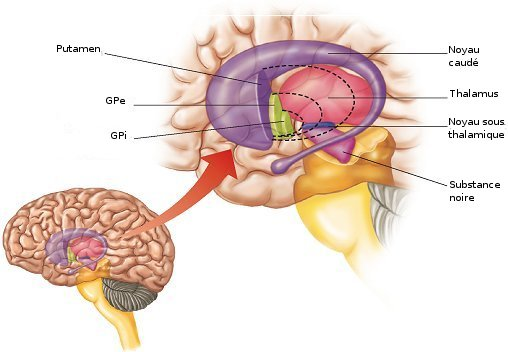
\includegraphics[width=0.6\textwidth]{figures/ch4_1_BG1}
  \end{center}
  \caption {Les différents noyaux des ganglions de la base. Le striatum (STR) composé du noyau caudé et du putamen. Le pallidum composé du segment interne (GPi) et segment externe (GPe). La substance noire composée de la partie compacte (SNc) et la partie réticulée (SNr). Le noyau sous thalamique (STN).} %Chevalier:1990,Deniau,}
  \label{fig:BG1}
\end{figure}


Ainsi, une caractéristique majeure de l'anatomie de \gls{bg} est leur implication dans plusieurs boucles avec le cortex cérébral (fig \ref{circuits}), appelées \textit{circuits cortico-basalo-thalamo-corticaux} \cite{Alexander:1986, Alexander:1990, Strick:1995}. Nous allons d'abord décrire les différents noyaux, ensuite, nous examinerons les différentes boucles.\\

\subsection {Anatomie}

\subsubsection{Le striatum}

Le striatum [\gls{str}] est le plus grand des noyaux gris centraux (à peu près $10^6$ neurones chacun connecté à $10^3$ synapses corticales). Il est composé du noyau caudé, du putamen et d'une partie différenciée connue sous le terme \textit{striatum ventral}\footnote{Le striatum ventral est particulièrement impliqué dans la régulation des comportements motivés comme les processus naturels liés à l'obtention d'une récompense ou les processus pathologiques de l'addiction. %(Ikemoto and Panksepp, 1996; Koob, 1992; Koob and Bloom, 1988; Robbins et al., 1989; Robledo and Koob, 1993; Robledo et al., 1992; Salamone, 1994
} qui englobe le noyau accumbens septi [\gls{nacc}], les parties ventromédiales du noyau caudé et du putamen et les cellules striatales des bulbes olfactives.\\

Le \gls{str} reçoit en effet de multiples afférences excitatrices glutamatergiques\footnote{Le glutamate, forme ionisée de l'acide glutamique, est le neurotransmetteur excitateur le plus important du système nerveux central.} qui proviennent globalement de toutes les aires du cortex cérébral sauf l'aire visuelle primaire V1 et l'aire auditive primaire [\gls{a1}] \cite{Albin:1995, Gerfen:1990, Kemp:1970, Cherubini:1988}. Le \gls{str} reçoit des entrées corticales liées aux paramètres des comportements \cite{Bauswein:1989,Turner:2000,Crutcher:1990}, liées au contexte \cite{Kimura:1990,Kimura:1992} et d'autres liées à la récompense \cite{Kawagoe:1998}. En outre du cortex, il reçoit des projections excitatrices des structures sous-corticales: thalamus [\gls{th}], hippocampe et amygdale \cite{Lapper:1992, Sadikot:1992}.\\ 

Au niveau microstructural, le \gls{str} peut être divisé en deux compartiments, le compartiment des \textit{striosomes} et celui des \textit{matrisomes} dont les connexions anatomiques sont distinctes\footnote{cette distinction entre matrisomes (matrices) et striosomes est encore un sujet de controverse et de même pour la distinction entre les récepteurs D1 et D2 décrits dans la suite}. Les connexions afférentes aux striosomes sont principalement issues du cortex orbital et des
régions limbiques (cingulaires et amygdaliennes). Le compartiment des matrices est innervé par les régions associatives (temporales, pariétales et préfrontales) et sensorimotrices du cortex. La voie striatonigrale décrite plus loin dans le texte réunit les neurones efférents des striosomes et se projette sur la substance noire compacte.\\

Plus généralement, le \gls{str} est constitué principalement de neurones épineux moyens [\gls{msn}] GABAergiques\footnote{L'acide $\gamma$-aminobutyrique, abrégé en GABA, est le principal neurotransmetteur inhibiteur du système nerveux central chez les mammifères et les oiseaux.} ($>90\%$). Au repos, ces neurones ont peu d'activité spontanée. Ils sont maintenus dans un état de faible excitabilité et sont peu réactifs aux influx corticaux excitateurs \cite{Nisenbaum:1995}. En conséquence, une forte activité synchronisée des projections cortico-striatales est nécessaire pour que les neurones de projection du striatum dépassent le seuil d'activation \cite {Mahon:2001, Mahon:2003}.\\

Ces neurones projettent d'une part sur le segment interne du pallidum [\gls{gpi}] et la substance noire réticulée [\gls{snr}]. D'autre part, ils projettent sur le noyau sous-thalamique [\gls{stn}] à travers le segment externe du pallidum [\gls{gpe}]. Les neurones qui projettent vers un noyau ou un autre sont morphologiquement indifférenciables et topographiquement mélangés  \cite {Feger:1984, Gerfen:1988, Parent:1989}. Ils commencent à décharger avant que le mouvement ne commence. Ceci suggère que le striatum participe à la programmation du mouvement volontaire. \cite{Lidsky:1985} ont signalé une activité neuronale striatale qui semblait être liée uniquement à des mouvements ou des stimuli sensoriels qui se produisent dans un contexte particulier. En effet, le \gls{str} participe à filtrer les informations corticales les plus pertinentes et transformer les signaux corticaux selon le contexte afin d'inhiber localement les noyaux de sorties des \gls{bg}. Il est principalement impliqué dans l'apprentissage de compétences motrices, perceptives et cognitives\cite{Joel:1994, Suzuki:2001}. \\

\subsubsection{Le pallidum externe}

Le segment externe du pallidum est une structure intermédiaire qui reçoit des projections inhibitrices du \gls{str} et d'autres excitatrices du \gls{stn} et renvoie des projections GABAergiques inhibitrices vers le \gls{str} et le \gls{gpi} mais majoritairement vers le \gls{stn} \cite{Rouzaire:1980}. Il semble agir en opposition aux projections striatales \cite{Alexander:1990}.\\


\subsubsection{Le pallidum interne et la substance noire réticulée}

Ces deux noyaux composés de neurones similaires sont considérés comme une seule structure fonctionnelle de sortie \cite {Carpenter:1981}. Ils sont toniquement actifs, i.e déchargent au repos à des taux élevés en l'absence de l'entrée striatale leur imposant une pause ou une réduction de leur cadence de décharge. L'effet net de l'entrée du striatum au \gls{gpi}/\gls{snr} est une réduction de l'inhibition tonique exercée par les cellules pallidales sur leurs cibles (désinhibition) permettant donc une augmentation du taux de décharge dans les cellules correspondantes (thalamus, colliculus supérieur...). Donc leur désinhibition permet en particulier d'activer les aires motrices via le thalamus par excitations glutamatergiques des aires corticales frontales et d'initier ainsi les mouvements moteurs bloqués toniquement \cite{Nauta:1966}.\\


\subsubsection{Le noyau sous-thalamique}

Le noyau sous-thalamique est le seul noyau excitateur des \gls{bg}, il re\c coit des projections inhibitrices du \gls{gpe} et ses neurones glutaminergiques renvoient des projections excitatrices répandues\footnote{efférences divergentes: chaque axone du \gls{stn} innerve de nombreux neurones du \gls{gpi}} (diffuses) au \gls{gpi} et à la \gls{snr} \cite{Parent:1993} permettant ainsi d'inhiber les générateurs de motifs moteurs [\glspl{mpg}] des mouvements concurrents. Il reçoit aussi des afférences excitatrices principalement des aires motrices du lobe frontal \cite{Monakow:1978,Kitai:1981,Nambu:1996,Nambu:1997}. L'entrée corticale vers le \gls{stn} est principalement liée au mouvement \cite{Delong:1985,Wichmann:1994}.\\

\subsubsection{La substance noire compacte}

Alors que la \gls{snr} est composée de neurones GABAergiques, la \gls{snc} est composée plutôt de neurones dopaminergiques qui projettent principalement sur les \glspl{msn} dans le \gls{str}. On parle donc de la voie nigro-striatale \cite{Haber:2000}. Au niveau dorsomedian de la \gls{snr} se trouve l'aire tegmentale ventrale, compos\'ee de neurones dopaminergiques identiques à ceux de la \gls{snc}. Ces neurones sont qualifiés ainsi parce qu'ils produisent un neuro-modulateur appelé \textit{la dopamine} [\gls{da}]. Le rôle de la dopamine au sein des \gls{bg} est complexe et en grande partie non résolu. \\

\begin{figure}
  \begin{center}
    \includegraphics[width=0.65\textwidth]{figures/ch4_2_dopamine}
  \end{center}
  \caption { Les neurones dopaminergiques signalent une récompense inattendue ou une absence inattendue de récompense \protect\cite{Schultz:1997}. (A) Si une récompense arrive de manière inattendue, l'activité du neurone dopaminergique augmente. (B) Si une récompense arrive suite à un stimulus la prédisant appris par le singe, l'activation n'est pas modifiée, signalant ainsi que tout se déroule normalement. (C) Si suite à un stimulus prédisant la récompense, rien ne se produit (pas de récompense), la décharge neuronale est inhibée.}
  \label{dopamine}
\end{figure}

Globalement, la dopamine est impliquée dans deux fonctions fondamentales du cerveau: activation motrice et apprentissage par récompense des associations stimulus-réponse (S-R). Il s'agit de choisir une action en réponse à un contexte sensoriel donné. Son effet de base est d'agir sur l'activité du striatum en projetant sur les récepteurs dopaminergiques D1 et les récepteurs D2 des neurones striataux. En effet, la dopamine excite les récepteurs D1 et inhibe les récepteurs D2. Avec l'action de la dopamine, la réponse de ces neurones à une entrée corticale est modifiée de telle sorte que les profils de l'activité striatale qui se corrèlent avec l'exécution des tâches suivies de récompense sont renforcés par l'augmentation de la force (poids) synaptique des entrées corticales.\\

La dopamine a d'abord été considérée comme un signal de récompense. Plusieurs enregistrements électrophysiologiques, chez des singes apprenant des tâches comportementales, ont montré des neurones dopaminergiques qui déchargent de façon phasique quand une récompense inattendue arrive mais quand la même expérience est répétée plusieurs fois, la décharge se décale dans le temps pour répondre aux stimuli prédisant ainsi la récompense et ne plus coïncider donc avec la récompense. La dopamine est ainsi considérée comme un signal d'erreur de récompense (corrélée donc avec l'anticipation de la récompense) et non plus un signal de récompense \cite{Houk:1995, Schultz:1997, Hollerman:1998, Morris:2004, Takikawa:2004, Bayer:2005,Schultz:2006} (fig \ref{dopamine}). Mais une grande partie de l'activité de la \gls{snc} semble être tonique plutôt que phasique ou transitoire, ce qui rend difficile d'établir la contribution explicite de cette voie à la commande motrice.\\

%\cite{Doya 1999}La dopamine code pour le prediction de la récompense $DA(t)=r(t)+1/[(V(t+1)-V(t)]$ \cite{Schultz 1997}.
%La plasticité dépend de la dopamine \cite{wickebs:1995}

\subsection{Organisation en boucles fonctionnelles}

%L'entrée corticale vers \gls{bg} est organisée en bandes longitudinales de projections parallèles. 

Les \gls{bg} semblent fonctionner via un système de boucles parallèles initialement décrites comme cinq circuits dissociés et parallèles: un circuit moteur qui inclut les aires motrices, prémotrices et motrices supplémentaires, un circuit oculomoteur passant par les champs oculaires frontaux [\glspl{fef}], deux circuits préfrontaux passant respectivement par le cortex dorsolatéral préfrontal et orbitofrontal latéral et finalement un circuit limbique reliant le cortex cingulaire et orbitofrontal médian \cite{Alexander:1990, Alexander:1986, Albin:1989,Mink:1996}. Cette forme d'organisation est particulièrement adaptée pour des effets de rétroaction (\textit{feed-back}) et d'anticipation (\textit{feed-forward}). Ces boucles permettent de sélectionner des états corticaux, de les intégrer et de contrôler leur succession \cite{Berns:1998, Beiser:1998, Hikosaka:1999, Nakahara:2001} (fig \ref{circuits}).\\


\begin{figure}
  \begin{center}
    \includegraphics[width=14cm,height=10cm]{figures/ch4_3_circuits}
  \end{center}
  \caption {Les différents circuits cortico-basalo-thalamo-corticaux. SNpr: substance noire réticulée, GPi: pallidum interne, PV: pallidum ventral, VAmc: noyau ventral antérieur du thalamus, VL: noyau ventro-latéral du thalamus, DM: noyau dorso-médian du thalamus, mc: magnocellulaire, pc: parvocellulaire, pm: paralamellaire, cl: caudolatéral, cdm: caudal dorsomédian, dl: dorsolatéral, l: latéral, ldm: latéral dorso-médian, m: médian, mdm: médian dorso-médian, pl: postéro-latéral, pm: postéro-médian, rd: rostro-dorsal, rl: rostro-latéral, rm: rostro-médian, vl: ventrolatéral, vm: ventromédian. [Adapté de \protect\cite{Alexander:1986}]}
  \label{circuits}
\end{figure}


Par la suite, ces cinq circuits ont été regroupés dans un modèle à trois circuits fonctionnels et distincts où chacun des \gls{bg} possède un compartiment sensorimoteur, un compartiment associatif et un compartiment limbique \cite{Parent:1990, Parent:1993,Joel:1994}. Des travaux chez le singe ont démontré, par micro-injections d'agents pharmacologiques, des réponses comportementales et une connectivité anatomique différente selon que l'un ou l'autre des compartiments est stimulé \cite{Grabli:2004}. Les trois circuits présentent la même organisation globale, les structures intermédiaires diffèrent en fonction du type de l'information traitée. Cette description postule donc que chacune des boucles met en jeu des subdivisions différentes dans chacune des structures des \gls{bg}. \\ 

Même si ces descriptions insistent sur la séparation entre les différentes boucles, les interférences entre elles peuvent être cruciales pour les activités corrélées dans les différentes régions corticales. En effet, les patients parkinsoniens sont également altérés dans le traitement et l'utilisation des informations proprioceptives. En règle générale, ils ont du mal  à coordonner et intégrer les différentes composantes élémentaires du mouvement en vue d'aboutir à un mouvement composé volontaire performant \cite{Schettino:2006}. Si le sujet dans l'exemple précédent, choisit de prendre le verre d'eau, ceci active le cortex frontal qui à son tour projette sur le cortex moteur qui détermine sa trajectoire en fonction du retour du cortex visuel. Puis le mouvement est déclenché en coordonnant la séquence de muscles à activer au cours du mouvement.\\

Ceci suggère que les \gls{bg} facilitent la liaison entre les différentes régions corticales qui agissent de manière coordonnée pour façonner le comportement moteur et participent à la planification\footnote{la planification cognitive est l'une des fonctions exécutives qui comprend les processus neurologiques impliqués dans la formulation, l'évaluation et la sélection d'une séquence de pensées et d'actions pour atteindre un objectif souhaité.} des comportements moteurs pour l'exécution de tâches complexes \cite{Elsinger:2006, Wu:2005, Houk:1995}. La perturbation des circuits neuronaux, par l'intermédiaire de divers mécanismes tels que des lésions cérébrales traumatiques, ou les effets des maladies neuro-dégénératives entre cette région du cortex frontal et les ganglions de la base, spécifiquement le striatum (voie cortico-striatale), peuvent perturber les processus nécessaires à la planification \cite{Houk:1995} mais nous ne nous intéresserons pas à cette fonction et seules des tâches simples seront considérées. Nous passerons en revue les différentes fonctions des \gls{bg} proposées dans la littérature pour s'intéresser en particulier au circuit moteur et son rôle dans la sélection de l'action.\\

%%%%%%%%%%%%%%%%%%%%%%%%%%%%%%%%%%%%%%%%%%%%%%%%%%%%%%%%%%%%%%%%%%%%%%%%%%%%%%%%%%%%%%%%%%%%%%%%%%%%%%%%%%%%%%%%%%%%%%%%%%%%%%%%%%%%%%%%%%%%%%%%%%%%%%
\subsection{Fonctions des ganglions de la base}

Les ganglions de la base sont essentiellement connus pour leur rôle dans le contrôle moteur, mais leur fonction ne se limite pas au traitement de l'information sensorimotrice, ils participent également à diverses fonctions cognitives et comportementales \cite{Middleton:2000}.\\

\subsubsection{Fonctions motrices : architecture du circuit moteur}

Le circuit moteur des \gls{bg} est le mieux étudié. Il se base sur les projections des aires corticales frontales associatives, principalement les régions prémotrice et motrice supplémentaire et le cortex préfrontal dorsolatéral sur le striatum antérieur. Une fois l'information traitée dans les \gls{bg}, elle est transmise via le thalamus moteur vers le cortex préfrontal et prémoteur. Les \gls{bg} modulent à la fois le système moteur latéral ( mouvements volontaires) et le système moteur médian (posture et tonicité des muscles).\\

En effet, une grande partie de l'entrée des \gls{bg} arrive au niveau de striatum qui projette vers la sortie \gls{gpi}/\gls{snr} via deux chemins : la ``voie directe'' et la ``voie indirecte'', qui semblent avoir des effets contraires \cite{Albin:1989} (détaillés dans la section suivante). Au repos, le thalamus est inhibé par \gls{gpi}/\gls{snr}. L'inhibition de certains neurones peut être enlevée sélectivement via la voie directe: le striatum inhibe certains neurones de \gls{gpi}/\gls{snr}. La boucle qui relie le néocortex, le striatum, le palladium interne, le thalamus et le cortex frontal est classiquement considérée comme la boucle principale des ganglions de la base. Mais il s'y ajoute la projection en aval de la substance noire réticulée principalement vers le colliculus supérieur, participant ainsi au contrôle oculomoteur des saccades visuelles \cite{Graybiel:1978, Hikosaka:1983a, Hikosaka:1983b, Hikosaka:1983c}.\\

A cette boucle principale, s'ajoutent aussi des boucles latérales qui participent particulièrement à la régulation de l'activité du palladium, comme la voie indirecte qui module la sortie des \gls{bg} \cite{Percheron:1991}. Une fois stimulés par le cortex, les neurones du striatum dans les axones de la voie indirecte envoient des projections inhibitrices sur les cellules du pallidum externe, qui inhibe de manière tonique le noyau sous-thalamique. Cette inhibition (par le \gls{str}) des projections inhibitrices du \gls{gpe}, se traduit par une réduction nette de l'inhibition du \gls{stn}. Finalement le \gls{stn}, à son tour, envoie des projections excitatrices au complexe \gls{snr}/\gls{gpi} (qui inhibe toniquement le thalamus). Le résultat final est en particulier une inhibition du thalamus et, par conséquent, une diminution de la stimulation du cortex moteur par le thalamus et l'activité musculaire est réduite.\\

Cette distinction de voies est surtout étudiée dans le circuit moteur et elle se base sur les cibles des projections des neurones striataux et leur sensibilité à la dopamine. Il est classiquement considéré que la voie directe contient des récepteurs D1 et la voie indirecte contient des récepteurs D2 \cite{Ince:1997, Gerfen:1995, Bloch:1994, Gerfen:1994} mais certaines études favorisent l'existence des deux types de récepteurs dans les deux voies \cite{Aizman:2000,Surmeier:1996}. Comme introduit dans \cite{Frank:2005}, on distingue donc deux types de signaux : le \textit{``GO signal''} qui sélectionne l'action adéquate à exécuter en réponse à un stimulus et le \textit{ ``NO-GO signal''} qui au contraire supprime une réponse. Cette distinction est fondée sur les activations neuronales qui ont été remarquées dans le striatum chez le singe en réponse à deux stimuli (clés) qui indiquent si le singe doit exécuter (GO) ou supprimer (NO-GO) un mouvement du bras \cite{Apicella:1992}. L'augmentation de la dopamine cause une augmentation du contraste entre les deux chemins et par conséquent sur les niveaux des signaux GO/NO-GO servant plus tard à diriger un apprentissage synaptique.\\

En considérant en plus l'entrée corticale vers le noyau sous-thalamique \cite{Mink:1993,Kita:1994, Mink:1996, Nambu:2000}, à ces deux voies s'ajoute la \textit{``voie hyperdirecte''} \cite{Nambu:2002, Joel:1997, Gerfen:2000}. Une stimulation corticale induit une excitation à courte latence, suivie par une inhibition puis une excitation retardée dans les neurones pallidaux de singes. L'excitation précoce est considérée comme provenant de la voie cortico-\gls{stn}-pallidiale (hyperdirecte) comme argumenté dans \cite{Nambu:2000}. Cette voie s'avère être une voie excitatrice rapide par opposition à celles qui passent par le striatum et qui semblent être plus lentes. Le modèle de Nambu qui introduit cette voie propose de considérer que lorsqu'un mouvement volontaire est présenté au niveau cortical, un premier message via la voie hyperdirecte excite de manière diffuse la \gls{snr}/le \gls{gpi} et par conséquent inhibe le thalamus et ses projections corticales. Cette inhibition est globale (non locale), il s'agit d'un signal de réinitialisation,\textit{``RESET''}. L'effet résultant est un effet {\em center-surround}: une sélection focalisée sur l'action adéquate avec une inhibition des commandes motrices compétitives \cite{Mink:1993, Mink:1996,Hikosaka:2000, Chevalier:1990, Hikosaka:1988}. \\

Des enregistrements de l'activité neuronale au niveau du \gls{gpi} montrent un comportement tri-phasique dont l'interprétation donne un éclairage sur le rôle des \gls{bg} dans l'initiation des mouvements. D'abord une augmentation de l'inhibition tonique juste après la stimulation du cortex somatomoteur (voie rapide hyperdirecte), suivie d'une baisse d'activité (voie directe) pour finir à nouveau par une hausse d'activité (voie lente indirecte) au niveau d'un neurone du \gls{gpi} \cite{Nambu:2008}.\\

Ces différentes voies agissent donc comme une balance réglable qui contrôle finement le niveau d'activation de la sortie des noyaux gris centraux. Un bon équilibre est nécessaire pour un fonctionnement moteur normal. En effet, l'activation sélective des différents éléments de ces voies détermine les activités spécifiques qui vont s'exprimer tandis que les autres sont fortement inhibées. Il en résulte deux types de sélection par compétition entre les voies \cite{Hikosaka:1993}. D'une part, une compétition simultanée: une inhibition globale via les voies indirecte et hyperdirecte contre une désinhibition sélective via la voie directe. D'autre part, une compétition séquentielle due aux différences entre les constantes temporelles des différentes projections. Plus généralement, pour générer un mouvement, il n'est pas suffisant d'activer le \gls{mpg} responsable de l'action souhaitée à cause de la présence de \glspl{mpg} concurrents qui sont préalablement activés et doivent se désactiver \cite{O:2006,Redgrave:1999}. Donc la première fonction motrice des \gls{bg} consiste à sélectionner le mouvement à effectuer en désinhibant le thalamus d'une part et supprimer toutes les autres actions concurrentes d'une autre part. \\

Rappelons que les structures de sortie de \gls{bg} projettent aussi sur le colliculus supérieur (qui à son tour projette sur le thalamus), donc inhibent de manière similaire les mouvements des yeux. D'après les études de saccades chez les singes, l'activité tonique des neurones de la \gls{snr} inhibe les neurones colliculaires qui contrôlent les saccades oculaires. Lorsque les neurones striataux de la voie directe sont excités par les champs oculaires frontaux, certains neurones de la \gls{snr} sont momentanément inhibés libérant ainsi les neurones colliculaires appropriés pour signaler la cible du mouvement oculaire. Le singe déplace alors son regard vers un nouvel emplacement.\\ 

Plus généralement, les \gls{bg} assurent qu'un seul programme moteur, parmi les programmes primitifs possibles, soit actif à un moment donné en inhibant tout conflit et toute concurrence. Ce programme est libéré temporairement ce qui lui permet d'être exécuté par le corps. Ainsi, les \gls{bg} agissent comme un interrupteur qui permet l'exécution de programmes automatiques et sont considéré donc comme un substrat de sélection de l'action motrice\cite{Kropotov:1999,Mink:1996,Redgrave:1999, Prescott:2007,Gurney:2001a, Frank:2005}. \\

\subsubsection{Fonctions cognitives}

Comme mentionné précédemment, certains circuits impliquant les \gls{bg}, impliquent aussi le cortex associatif préfrontal et le cortex limbique. En plus de son rôle moteur, les \gls{bg} participent à plusieurs processus cognitifs et fonctions sensorielles (motivation, sélection, mémoire, apprentissage ...) \cite{Berns:1996,Redgrave:1999}. Certaines personnes atteintes de la maladie de Parkinson souffrent de déficits cognitifs tels que la suppression visuelle et les problèmes de reconnaissance des visages \cite{Jacobs:1995}. D'autres patients présentant des lésions du pallidum ou de la \gls{snr} ont des troubles de mémoire de travail, un comportement obsessionnel et des hallucinations visuelles \cite{Laplane:1989}. En particulier, l'implication des \gls{bg} dans la mémoire de travail peut être considérée comme une extension de son rôle dans la sélection de l'action \cite{Prescott:2003, Kawagoe:1998}. \\

En outre, les \gls{bg} semblent être impliqués dans certaines tâches d'apprentissage comme la mémorisation des associations stimuli/réponses \cite{Hikosaka:1998, Perez:2001}. Les patients Parkinsoniens n'arrivent pas à réussir de telles tâches \cite{Knowlton:1996}.  Des enregistrements de neurones striataux chez les singes ont montré que les propriétés de l'activation du striatum changent lorsqu'une association est construite entre un stimulus sensoriel spécifique et une réponse motrice appropriée \cite{Aosaki:1994}.\\


D'autres formes d'apprentissage semblent également être influencées par les \gls{bg}. Des études physiologiques ont montré que des parties du striatum et du pallidum sont activées pendant l'exécution des tâches qui nécessitent l'apprentissage d'une séquence de mouvements \cite{Kermadi:1995, Cromwell:1996,Berns:1998}. L'apprentissage de séquences nécessite soit la présence d'une mémoire de travail assurée par un feedback local par exemple \cite{Smith:1994}, soit un feedback de la sortie des \gls{bg} vers le cortex mais cette voie semble être très lente \cite{Alexander:1986,Hedreen:1991}. C'est ainsi qu'une revue datant de 2000, \cite{Gillies:2000} classe les modèles computationnels des \gls{bg} en 3 familles : Les modèles de traitement séquentiel \cite{Berns:1998}, les modèles de sélection de l'action \cite{Gurney:2001a} et les modèles d'apprentissage par renforcement comme les travaux de \cite{Schultz:2000a, Schultz:2000b} en particulier les modèles d'acteur-critique \cite{Barto:1995,Houk:1995,Brown:1999,Suri:2001,Suri:1998,Contreras:1999}.\\

Ces derniers modèles considèrent les \gls{bg} comme une architecture permettant de prédire et d'évaluer la récompense à chaque pas de l'épisode de la simulation \cite{Joel:2002,Niv:2001}. Le principe est de choisir grâce à la partie ``acteur'', à partir des états courants et des connaissances actuelles, la meilleure action à faire en se basant sur les prédictions de la partie ``critique''. L'architecture acteur-critique fait partie des méthodes à base de \textit{différence temporelle (TD)} \cite{Samuel:2000,Klopf:1972,Sutton:1988, Houk:1995,Joel:2002} qui servent à résoudre des problèmes de prédiction (étant donné l'état actuel des variables, quel avantage ou récompense peut on espérer gagner dans le futur). Les erreurs de prédictions permettent d'adapter et de corriger les deux agents \cite{Sutton:1998}. L'analogie entre les \gls{bg} et les modèles d'acteur-critique s'appuie sur la forte ressemblance entre les activités des neurones dopaminergiques (fig \ref{dopamine}) et le signal d'erreur de prédiction ainsi que le fait que la plasticité synaptique dépend à long terme de la dopamine \cite{Calabresi:2000,Wickens:1996}. En effet, La dopamine phasique (par opposition à la dopamine tonique) est supposée résulter de l'erreur dans le feedback moteur et servir à la modulation du seuil de facilitation ou de suppression des commandes motrices en réponse à un stimulus.\\
 
Certains modèles computationnels se concentrent sur le mécanisme d'apprentissage lui même sans s'intéresser à la structure du cerveau \cite{Perez:2001}. D'autres s'intéressent aux structures mais partiellement à l'apprentissage, soit à apprendre le signal d'erreur dopaminergique \cite{Brown:1999, Barto:1995}, soit à choisir des signaux d'erreur à la main pour apprendre des associations \cite{Frank:2005,Gurney:2001a,Berns:1998}. Par exemple, \cite{Frank:2005} propose un modèle qui apprend à choisir entre deux actions en réponse à un ensemble d'entrées. Les deux voies permettent d'apprendre les conditions du \textit{gating} (GO) et de la suppression (NO-GO). Ce modèle a été proposé comme une base théorique pour un apprentissage procédural des tâches cognitives. D'autres chercheurs se sont intéressés au codage de l'information de la récompense et à la sélection de la réponse dans la circuiterie biologique \cite{Brown:2004,Gurney:2001a,Beiser:1998} sans modéliser l'apprentissage implicite. Il en a résulté des modèles de critiques pour la prédiction et la simulation des effets de la dopamine \cite{Brown:2004} et des modèles d'acteurs détaillés pour des tâches de sélection avec une seule motivation \cite{Frank:2006,Khamassi:2004,Khamassi:2005} ou multimotivationnelles \cite{Dayan:2001,Girard:2008}.\\


Enfin, un rôle très peu étudié des \gls{bg} correspond à la {réduction de dimensionnalité} qui s'opère entre l'entrée des \gls{bg} et leur sortie basé sur des constatations anatomiques. Le nombre de neurones corticaux qui projettent sur le striatum est cent fois plus grand que le nombre de neurones striataux \cite{Kincaid:1998} avec une réduction supplémentaire identique au niveau du \gls{gpi} \cite{Percheron:1994}. Ensuite, on observe un élargissement en partant du \gls{gpi} vers le cortex en passant par le thalamus \cite{Arecchi:1996,Sidibe:1997}. Des études théoriques ont montré que les réseaux de neurones réalisent des réductions de dimensionnalités par règles hebbiennes \cite{Oja:1982} pour les connexions intercouches et règles anti-hebbiennes pour les connexions latérales intracouches \cite{Foldiak:1989}. L'idée est de considérer les \gls{bg} comme un commutateur adaptatif central qui ordonne les informations entrantes selon les priorités et les compresse pour activer le cortex frontal à travers un nombre limité de canaux. Deux stratégies sont proposées, réduire la dimensionnalité [PCA,(\textit{Principal Component Analysis})] ou bien réduire l'information (voir \cite{Bar:2003} pour plus de détails). \\


Nous allons nous intéresser en particulier au rôle des \gls{bg} dans la sélection de l'action en considérant donc principalement le circuit moteur. Nous allons décrire d'abord quelques modèles existants mettant en oeuvre la sélection intrinsèque par désinhibition basée sur l'interaction entre plusieurs voies concurrentes, dans les \gls{bg}, pour expliciter dans la suite notre proposition.\\ 
%-------------------------------------------------------------------

\subsection{ Modèles computationnels du circuit moteur}

\subsubsection{Le modèle classique}

Un des premiers modèles de ganglions de la base est celui de Albin-Delong \cite{Albin:1989, DeLong:1990}. Il a été inspiré des troubles de mouvements chez les patients parkinsoniens. En effet, dans la maladie de Parkinson, qui est un trouble hypo-kinétique \footnote{les patients hypo-kinétiques sont plus lents que la normale, prennent plus de temps pour accomplir certaines tâches, génèrent moins de force. Les patients parkinsoniens sont également hypo-métriques et font des mouvements à amplitudes plus faibles que la normale en essayant d'atteindre une cible}, l'hyperactivité relative de la voie indirecte conduit à l'excitation excessive du \gls{gpi} (inhibiteur). De même dans la dystonie, qui est un trouble hyperkinétique, l'hyperactivité relative de la voie directe conduit à l'excitation réduite du \gls{gpi} (inhibition réduite du thalamus), donc à l'activation motrice involontaire. Ce modèle rend compte aussi du fonctionnement normal du système dans la régulation des mouvements, mais aussi du fonctionnement pathologique dans les syndromes hyper- et hypo-kinétiques. Selon ce modèle, les neurones striataux de la voie directe désinhibent leurs objectifs thalamo-corticaux permettant d'initier l'action désirée et ceux de la voie indirecte inhibent les actions non-désirées (fig\ref{Albin}-A).\\

\begin{figure}
\begin{center}
\includegraphics[width=0.8\textwidth]{figures/ch4_4_Bg3}
\end{center}
\caption{Organisation des connexions intrinsèques dans les noyaux gris centraux. A. La proposition influente par Albin et ses collègues (1989). La sortie des ganglions de la base est déterminée par l'équilibre entre les connexions inhibitrices directes (la voie directe) et la voie indirecte via des relais dans le pallidum externe (GPe) et le noyau sous-thalamique (STN). L'équilibre est supposé être réglé par des signaux dopaminergiques afférents de la substance noire compacte (SNc) agissant différemment sur les récepteurs de la dopamine D1 et D2. B. Des études anatomiques récentes ont révélé une organisation un peu plus complexe avec de nouvelles connexions.[Scholarpedia]}
\label{Albin}
\end{figure}

La voie dite ``directe'' est représentée par les projections directes, inhibitrices, GABAergiques du \gls{str} sur la \gls{snr} et le \gls{gpi}. Par cette voie, le striatum inhibe l'activité spontanée, tonique et inhibitrice et également GABAergique des structures de sortie des \gls{bg}. La voie dite ``indirecte'' comporte une étape supplémentaire impliquant successivement le \gls{gpe} et le \gls{stn} puisque le striatum renvoie également des projections GABAergiques inhibitrices vers le \gls{gpe} qui à son tour renvoie des projections GABAergiques inhibitrices vers le \gls{stn}. En inhibant les neurones GABAergiques du GPe, les neurones striataux projettant sur le \gls{gpe} désinhibent donc les neurones glutamatergiques du \gls{stn}. C'est ainsi que les neurones du \gls{stn} renforcent au final l'inhibition tonique que les structures de sortie des \gls{bg} exercent sur leurs cibles grâce à ses projections glutamatergiques excitatrices sur la \gls{snr} et le \gls{gpi}.\\

Il est considéré que la dopamine libérée à partir de la \gls{snc} agit sur deux sous-types de récepteurs dopaminergiques situés au \gls{str} et présentant des effets opposés. La dopamine aurait ainsi un effet global facilitateur sur la voie directe par l'intermédiaire des récepteurs D1 et inhibiteur sur la voie indirecte par l'intermédiaire des récepteurs D2.\\

Ce modèle a été appliqué à des mouvements des membres \cite{Mink:1996} et des mouvements des yeux \cite{Hikosaka:1993}, même si le circuit oculomoteur est un peu différent puisqu'il fait intervenir le colliculus supérieur, structure sous corticale \cite{McHaffie:2005}. Dans sa version de base, ce premier modèle ne prend pas en considération la voie hyper-directe, précédemment évoquée, qui comporte la projection corticale vers le noyau sous-thalamique sans passer par le striatum. Il considère ainsi que ce dernier est l'entrée corticale unique des \gls{bg}. En outre, il a été démontré que ce modèle a plusieurs lacunes et ne répond pas à certaines données cliniques et atomiques \cite{Parent:1998}.\\

En effet ce modèle ``classique'' ne prend en compte qu'une partie des connexions entre les \gls{bg} (fig \ref{Albin}-B) \cite{Parent:1998,Parent:2001}. Il ne considère pas les projections inhibitrices GABAergiques directes du \gls{gpe} sur la \gls{snr} et le \gls{gpi}. De même, il néglige les connexions réciproques entre le \gls{gpe} et le \gls{stn} \cite{Shink:1996}. Il est surtout reproché à ce modèle de considérer que l'information est transmise de manière séquentielle et unidirectionnelle depuis le striatum vers les structures de sortie des \gls{bg}.\\

\subsubsection{Le mod\`ele GPR}

Ensuite \cite{Redgrave:1999} se sont intéressés au rôle des \gls{bg} dans la sélection de l'action chez les vertébrés et ont proposé un modèle qualitatif de l'architecture des noyaux gris centraux. Ils ont expliqué les opérations de sélection de \gls{bg} et décrit le rôle de la dopamine dans le cadre de la sélection de l'action. Ils ont combiné les approches ascendantes (\textit{bottom-up}) et descendantes (\textit{top-down}) dans la modélisation des boucles à travers les noyaux gris centraux. Les modèles de l'approche ascendante partent de données biologiques pour définir l'architecture et les paramètres. En revanche, l'approche descendante part d'un problème comportemental et propose des théories fonctionnelles sur lesquelles seront basés les modèles. Selon leur étude qualitative un système neuronal, tels les \gls{bg}, ne peut être considéré comme le lieu d'un mécanisme de l'\gls{as} que s'il répond aux exigences suivantes: \\

\begin{itemize}
\item le système doit avoir l'information sur les facteurs influant la décision. Ces facteurs peuvent être internes à l'organisme ou provenant de l'environnement extérieur.
\item il faut un paradigme de calcul de la saillance comme ceux cités dans l'introduction.
\item il faut un mécanisme qui permet de résoudre le conflit entre les actions concurrentes. Citons l'exemple de l'inhibition récurrente réciproque. Dans ce mécanisme plusieurs unités connectées s'inhibent mutuellement formant une rétroaction positive. En effet, la hausse d'activité d'une unité provoque l'inhibition des autres et donc la diminution de l'effet inhibiteur de ces derniers sur cette unité et donc la sur-activation de celle-ci. 
\item la sortie du système permet d'exprimer l'action gagnante en éliminant les autres. L'exemple précédent l'assure puisque ce mécanisme permet d'augmenter le contraste entre plusieurs activations concurrentes et assure ainsi le gain de l'activation la plus importante.\\  
\end{itemize}

De nombreux modèles de calcul de \gls{bg} ont été proposés ensuite afin d'étudier le mécanisme de \textit{sélection par désinhibition} \cite{Chevalier:1990} dans les ganglions de la base (pour des revues voir \cite{Gillies:2000, Gurney:2004}). Parmi ceux-ci, nous nous sommes intéressés en particulier au modèle de \cite{Gurney:2001a,Gurney:2001b} qui a été testé comme mécanisme de sélection de l'action pour les agents autonomes en mesure par exemple de résoudre une tâche de survie minimale  \cite{Girard:2003, Girard:2005a, Gonzalez:2000, Prescott:2006}.\\

Les effets de la variation de la dopamine tonique provenant de la [\gls{vta}] sur la sélectivité du modèle ont été examinés \cite{Gurney:2001b} ainsi que son implication dans le contrôle de la balance entre les stratégies d'exploitation et d'exploration dans la sélection de l'action \cite{Humphries:2012}. La dopamine phasique impliquée dans l'apprentissage par renforcement (moduler en temps réel les saillances des actions) n'a pas été considérée et les saillances des actions ont été modulées à la main à partir des entrées sensorielles, proprioceptives et contextuelles.  \\

\begin{figure}
\begin{center}
\includegraphics[width=0.7\textwidth]{figures/ch4_5_gpr}
\end{center}
\caption{Les voies de sélection et de contrôle selon le modèle \protect\gls{gpr}. Les flèches pleines: connexions excitatrices. Les flèches en pointillés: connexions inhibitrices. STN: noyau sous-thalamique, Striatum D1: striatum avec récepteurs de dopamine D1, Striatum D2: striatum avec récepteurs de dopamine D2, GPe: pallidum externe, GPi: pallidum interne, SNr: substance noire réticulée. }
\label{GPR}
\end{figure}


Le modèle [\gls{gpr}] a donné une interprétation de l'architecture intrinsèque des \gls{bg} différente de l'interprétation classique basée sur le schéma d'Albin \cite{Albin:1989} (voie directe/voie indirecte). Les auteurs ont ajouté des voies à travers le \gls{gpe}, comme une boucle de régulation qui stabilise les voies de sélection dans les anciens modèles et améliore la sélectivité (fig\ref{GPR}). Ils considèrent donc deux voies, une voie de sélection et une voie de contrôle. La figure (fig. \ref{GPR}) montre les différentes connexions considérées dans le modèle. Les flèches continues représentent les projections excitatrices et les flèches discontinues les projections inhibitrices. Dans un article ultérieur, \cite{Humphries:2002} ont introduit un modèle computationnel du circuit cortico-basal-thalamo-cortical.\\

\subsubsection{Le mod\`ele CBG}

Un modèle modifié de \cite{Gurney:2001a} a été proposé par \cite {Girard:2008} de manière à améliorer ses caractéristiques dynamiques en utilisant la théorie analytique de contraction. En particulier, ce modèle [\gls{cbg}] prend en compte des projections, généralement négligées, entre le \gls{gpe} et le \gls{str} permettant d'améliorer son efficacité. Cette connexion \gls{gpe}-\gls{str} sert à faire taire les neurones striataux non choisis qui est en accord avec le fait que le striatum est connu pour être silencieux au repos \cite{Delong:1984}. Ce modèle néglige les projections du \gls{stn} vers le \gls{str} \cite{Parent:2000} ainsi que les connexions latérales dans le \gls{gpe} et le \gls{snr} \cite{Deniau:1982, Juraska:1977} qui sont ajoutées au modèle \gls{gpr} dans \cite{Gurney:2004}. La figure \ref{CBG} montre les connexions prises en compte par le modèle. Les flèches pleines désignent les connexions inhibitrices et les flèches vides désignent les projections excitatrices.\\

\begin{figure}
\begin{center}
\includegraphics[width=0.8\textwidth]{figures/ch4_6_CBG}
\end{center}
\caption{Le modèle \protect\gls{cbg}. Les flèches pleines désignent les connexions inhibitrices et les flèches vides désignent les projections excitatrices. STN: noyau sous-thalamique, Striatum D1: striatum avec récepteurs de dopamine D1, Striatum D2: striatum avec récepteurs de dopamine D2, GPe: pallidum externe, GPi: pallidum interne, SNr: substance noire réticulée, FS: neurones à décharge rapide (fast spiking) (tiré de \protect\cite{Girard:2008})}
\label{CBG}
\end{figure}

Comme dans le modèle \gls{gpr}, seule la dopamine tonique a été considérée et le mécanisme basique de sélection par désinhibition est conservé. En effet, dans les deux modèles \gls{gpr} et \gls{cbg} la sélection est basée sur des boucles locales récurrentes entre six canaux en compétition. Si l'entrée ne change pas au cours de la simulation, même si on perturbe l'activité au niveau du \gls{str}, le choix est déterministe et donc la saillance de l'action au niveau du \gls{pfc} est déterminante de l'action à choisir ({\em feedforward selection}). 


En s'inspirant de ces deux modèles, nous proposons un nouveau modèle de la boucle motrice des ganglions de la base en leur attribuant un rôle actif dans le calcul de la saillance et par la suite dans la sélection de l'action dépendant du contexte sensoriel, temporel et motivationnel. Nous avons modifié, supprimé et ajouté différentes projections afin de rendre compte du schéma de sélection que nous proposons. Nous détaillerons en premier lieu les caractéristiques de la version basique de notre modèle en le positionnant par rapport aux modèles précédemment évoqués. En deuxième lieu, les résultats des simulations seront discutés en évoquant la version complète utilisant l'apprentissage.\\  

\section{Conception et modélisation}

Le modèle de sélection motivée de l'action que nous proposons, inspiré des modèles \cite{Gurney:2001a, Girard:2008}, conserve le mécanisme basique de sélection intrinsèque par désinhibition. L'interaction entre plusieurs flux et différentes boucles récurrentes permettant de mettre en compétition une excitation diffuse et une inhibition locale à travers les différentes voies rend complexe la mise en oeuvre d'un modèle adaptatif et encore plus difficile la description de sa dynamique.\\
 
Nous proposons en particulier deux mécanismes supplémentaires. D'abord, un mécanisme d'évaluation de la saillance donne plus de liberté dans la détermination du choix de l'action, en considérant en particulier un feedback thalamique souvent négligé dans les boucles cortico-basales vers le striatum. Ce mécanisme permet de mettre en compétition ce qui est appris par l'habitude (projection cortex-cortex), ce qui est choisi par exploration (projection cortex-striatum) et ce qui est choisi par motivation (projection contexte-striatum). Ensuite, nous avons a mis en oeuvre un mécanisme adaptatif de création dynamique d'une représentaion du contexte (structure S), donc de création de méta-actions en faveur de l'approche énactive.\\%résultats

\subsection{Hypothèses}

L'architecture de base de notre modèle est similaire à celle de \cite{Gurney:2001a, Gurney:2001b, Girard:2005a, Girard:2008}. Nous utilisons le même type de neurones (intégrateur à fuite voir section 1) et chaque canal de \gls{bg} est représenté par une unité dans chacun des noyaux. On se situe donc dans le circuit moteur, chaque canal correspond donc à une action motrice.\\ 

Une différence principale par rapport à ces modèles est l'entrée du système qui n'est plus un vecteur pré-calculé de saillances. C'est un vecteur de perception sensorielle auquel est associé une pré-activation motrice correspondant aux actions candidates, réalisée par une sorte de mémoire de travail\footnote{C'est la capacit\'e \`a maintenir et \`a utiliser des repr\'esentations mentales pour les comportements orient\'es vers un but. Le cortex pr\'efrontal est réputé pouvoir réaliser des fonctions de m\'emoire de travail \cite{Petrides:1994, Cohen:1997}. Les \gls{bg} aussi, support\'es par des connexions anatomiques avec les aires corticales associatives.}. %Middelton_1994,Levy_1997,Owen_1996,Owen_1999}.
Une entrée représentant un contexte supplémentaire sera ajoutée dans une version traitée plus tard qui servira à apprendre à choisir des actions en fonction d'une consigne particulière et non pas seulement en fonction de son importance dans la mémoire de travail.\\

En effet, le cortex pariétal postérieur [\gls{ppc}] participe à l'évaluation du contexte sensoriel dans lequel s'effectue le mouvement. Le cortex pariétal évalue les différentes données comme la position du corps et de la cible dans l'espace grâce aux informations somatosensorielles, proprioceptives et visuelles qu’il reçoit. Il produit ainsi des modèles internes du mouvement à effectuer vers le cortex prefrontal [\gls{pfc}], en amont des cortex prémoteur et moteur. Ainsi dans notre modèle, une tâche de sélection commence par l'activation d'une unité du \gls{ppc} correspondant à un perception sensorielle donnée, qui à son tour, active un sous ensemble des unités du \gls{pfc} de manière inégale. Chaque unité active dans le \gls{pfc} correspond à une action candidate et une activation plus importante qu'une autre signifie que l'action concernée a été plus utilisée dans l'histoire et l'expérience de l'agent (les poids de projections entre le \gls{ppc} et le \gls{pfc} sont supposés être appris grâce à une règle hebbienne\footnote{Loi de Hebb :la force de la connexion (synaptique) présente entre deux neurones est augmentée durablement lorsque la décharge du neurone pré-synaptique (en amont de la synapse) est fortement corrélée temporellement à celle du neurone post-synaptique (en aval de la synapse) \cite{Hebb:1949}}).\\

L'hypothèse de fonctionnement en bandes parallèles dans les \gls{bg} se base sur un effet macroscopique. Comme il est nécessaire que les différents circuits impliquant les \gls{bg} communiquent, on peut supposer qu'au sein d'un circuit les canaux peuvent se rejoindre comme au niveau du \gls{stn} et on peut utiliser des projections diffuses du \gls{ppc} vers le \gls{str} (i.e. le \gls{ppc} renvoie une excitation supplémentaire vers toutes les cellules striatales). Nous supposons que cette projection corticale prépare l'activation d'unités striatales qui correspondent aux actions candidates. En effet, le \gls{str} est toniquement silencieux et a donc besoin d'être fortement stimulé pour que les neurones striataux arrivent à leur seuil d'activation. Il reçoit aussi des projections excitatrices du \gls{pfc}. \\ 

On ne distingue pas les neurones selon leurs sensibilités à la dopamine donc on ne considérera pas de subdivisions internes au striatum. En effet, on ne s'intéresse pas à la dopamine tonique ce qui revient à moduler les poids des projections entre le \gls{str} d'une part et le \gls{gpe} et le \gls{gpi} d'une autre part. En plus les neurones qui projettent vers le \gls{gpi} et le \gls{gpe} sont morphologiquement et topographiquement indifférenciables dans le \gls{str} donc on a choisi de ne pas tenir compte de la différence des récepteurs de dopamine \cite{Gerfen:1990} (d'autant plus que ce sujet est controversé dans la littérature). Le \gls{str} reçoit aussi des projections excitatrices du \gls{pfc}, d'autres inhibitrices du \gls{gpe}. On suppose en plus la présence d'une activité parasite faible, un bruit $N$  qui vient perturber l'activité striatale sans pouvoir dépasser le seuil d'activation $e_{\gls{str}} $. Ainsi l'entrée du \gls{str} est décrite par l'équation suivante. Nous avons ajouté un feedback thalamique provenant plus particulièrement du thalamus ventro-latéral [\gls{vlt}] ${\gls{vlt}}_{Out}$  qui va renforcer le choix fait par la partie intrinsèque des ganglions de la base, qui peut être différent de celui pré-imposé par la pré-activation au niveau du \gls{pfc}.\\

\begin{center}
\begin{equation} 
\gls{str}_{In}= {\gls{ppc}}_{Out}+{\gls{pfc}}_{Out}-{\gls{gpe}}_{Out}+{\gls{vlt}}_{Out}-e_{\gls{str}}+N
\end{equation}
\label{eqstr}
\end{center}

En effet, dans les modèles \gls{gpr} et \gls{cbg} la sélection est déterministe, le plus fort gagne la compétition. Pour passer à une sélection active et pouvoir intégrer un mécanisme d'apprentissage, un retour post-moteur est nécessaire d'où l'intérêt d'intégrer la projection excitatrice glutamatergique des noyaux thalamiques vers le \gls{str} \cite{Lapper:1992, Sadikot:1992}.\\

D'autre part, nous avons ajouté une inhibition latérale $L$ lente au niveau du \gls{pfc} qui va s'ajouter à l'excitation récurrente avec le thalamus pour finalement permettre d'avoir à la fin de la simulation une seule action active (prémotrice). Ceci permet d'installer un apprentissage hebbien entre le \gls{ppc} et le \gls{pfc} d'une part et d'autre part renforce la sélection au niveau du \gls{str} et permet d'installer un apprentissage par renforcement en se basant sur la sortie du \gls{str} et non pas seulement sur la sortie du \gls{gpi}. Globalement, à la différence de \gls{gpr} et \gls{cbg}, nous visons une sélection nette à tous les niveaux de la boucle et non pas seulement au niveau du \gls{gpi}. D'où l'équation de l'entrée du \gls{pfc}:

\begin{center}
\begin{equation} 
{\gls{pfc}}_{In}= {\gls{ppc}}_{Out}+{\gls{vlt}}_{Out}-e_{\gls{pfc}}+L
 \end{equation}
\end{center}

Comme dans le modèle \gls{cbg}, le noyau sous-thalamique reçoit seulement du \gls{pfc}, entrée excitatrice des aires motrices du lobe frontal \cite{Mink:1996} et le \gls{str} reçoit de toutes les aires du cortex cérébral \cite{Cherubini:1988, Kemp:1970}. Il reçoit aussi des projections inhibitrices du \gls{gpe}. Son activité tonique est modulée par un seuil d'activation négatif $e_{\gls{stn}}$ d'ou l'équation suivante:

\begin{center}
\begin{equation} 
{\gls{stn}}_{In}= {\gls{pfc}}_{Out}-{\gls{gpe}}_{Out}-e_{\gls{stn}}
 \end{equation}
\end{center}

Le \gls{gpe} et le \gls{gpi} sont des noyaux inhibiteurs. De même que dans \gls{cbg} et \gls{gpr}, ils reçoivent des afférences sélectives du \gls{str} et une
excitation diffuse du \gls{stn}. On néglige la projection entre le \gls{gpe} et le \gls{gpi} puisque la sortie GABAergique inhibitrice du \gls{gpe} est majoritairement vers le \gls{stn} \cite{Rouzaire:1980} et le fait de l'ajouter ne modifie pas les résultats des simulations puisque les poids peuvent être réadaptés: 

\begin{center}
\begin{equation} 
{\gls{gpe}}_{In}= {\gls{stn}}_{Out}-{\gls{str}}_{Out}-e_{\gls{gpe}}
 \end{equation}
\begin{equation} 
{\gls{gpi}}_{In}= {\gls{stn}}_{Out}-{\gls{str}}_{Out}-e_{\gls{gpi}}
 \end{equation}
\end{center}

Le \gls{gpi} et la \gls{snr} sont considérés comme une seule structure fonctionnelle de sortie puisqu'elles possèdent des neurones similaires et historiquement étaient une seule entité \cite{Carpenter:1981}. Et finalement l'équation du noyau \gls{vlt} qui est sous inhibition tonique du \gls{gpi} et en excitation réciproque avec le \gls{pfc} s'écrit:

\begin{center}
\begin{equation} 
{\gls{vlt}}_{In}= {\gls{pfc}}_{Out}-{\gls{gpi}}_{Out}-e_{\gls{vlt}}
 \end{equation}
\end{center}

Il en résulte donc l'architecture présentée dans la figure \ref{TBG0}.

\begin{figure}
\begin{center}
\includegraphics[width=0.5\textwidth]{figures/ch4_7_TBG_00}
\end{center}
\caption{L'architecture de notre modèle de la boucle cortico-basale. Les connexions excitatrices (glutamergiques) sont représentées par des flèches pleines, les connexions inhibitrices (GABAergiques) par des flèches en pointes rondes. En l'absence de stimuli, donc au repos, le \protect\gls{gpe} et le \protect\gls{gpi} sont toniquement actifs. La struture S sera décrite dans la suite.}
\label{TBG0}
\end{figure} 

\subsection{Simulation et résultats}

\subsubsection{Scénario sans apprentissage}

De même que pour les simulations effectuées par les auteurs de modèles \gls{gpr} et \gls{cbg}, nous avons utilisé un modèle à six canaux. Les paramètres ont été fixés à des valeurs résumées en annexe. La simulation a été programmée en python, en utilisant la simple approximation d'Euler (voir chapitre 1) pour l'intégration, avec un pas de temps de 1 ms. \\

Nous avons simulé avec notre modèle un test de sélection simple similaire à celui de \cite{Gurney:2001b} et avec la version du modèle \gls{gpr} présentée dans \cite{Prescott:2006} et reproduite dans \cite{Girard:2008}. La sélection concerne deux canaux d'actions dont les pré-activations au niveau du \gls{pfc} valent 0.4 et 0.6 via une activation du \gls{ppc}. Une simulation dure 2 secondes suivie de 2 secondes de repos pour éviter l'effet de mémoire courte (l'activité forte d'un canal est maintenue jusqu'à ce que le stimulus soit enlevé, et donc peut influencer la prochaine sélection). On représente la même entrée plusieurs fois et on enregistre les profils d'activités des canaux concernés (fig \ref{TBG4}). Nous avons fait un test semblable en implémentant les deux modèles \gls{gpr} (fig \ref{GPR4})et \gls{cbg} (fig \ref{CBG4}) avec la même séquence de simulation et un vecteur de saillance d'entrée (0.4,0.6,0,0,0,0) pour comparer les effets.\\
\begin{figure}
\begin{center}
\includegraphics[width=\textwidth]{figures/ch4_8_model_04}
\caption{ Test de sélection entre deux canaux par notre modèle. L'entrée du modèle: On suppose qu'une cellule (la première par exemple) de PC est activée à 1 (n'est pas représentée dans les figures) et qui projette sur PFC avec deux poids différents sur les canaux 0 et 1 (0.4 pour le canal 0 et 0.6 pour le canal 1). Les courbes (A,B,C,D,E,F,G,H,I,J,K,L) représentent l'évolution de l'activité dans le temps dans les deux premiers canaux (lieux de compétition) qui commence par une période de repos (entrée nulle pendant 2s) suivie de 4 simulations (de durée 2s) alternées avec des périodes de repos. Les diagrammes (1,2,3,4,5,6) représentent les niveaux d'activités à la fin d'une simulation dans les 6 unités de chaque structure (les niveaux d'activités sont entre 0 et 1). }
\label{TBG4}
\end{center}
\end{figure}
\begin{figure}
\begin{center}
\includegraphics[width=\textwidth]{figures/ch4_9_girard_04}
\caption{ Test de sélection entre deux canaux par le modèle \protect\gls{cbg}. L'entrée du modèle: les deux premiers canaux de PC sont activés à 0.4 et 0.6 simultanément. Les courbes (A,B,C,D,E,F) représentent l'évolution de l'activité dans le temps dans les trois premiers canaux au niveau de \protect\gls{gpi} et \protect\gls{pfc} qui commence par une période de repos (entrée nulle pendant 2s) suivie de 4 simulations (de durée 2s) alternées avec des périodes de repos. Les diagrammes (1,2,3,4,5,6,7,8,9) représentent les niveaux d'activités à la fin d'une simulation dans les 6 unités de chaque structure.}
\label{CBG4}
\end{center}
\end{figure}
\begin{figure}
\begin{center}
\includegraphics[width=\textwidth]{figures/ch4_10_gurney_04}
\caption{ Test de sélection entre deux canaux par le modèle \protect\gls{gpr}. L'entrée du modèle: les deux premiers canaux de PC sont activés à 0.4 et 0.6 simultanément. Les courbes (A,B,C,D,E,F) représentent l'évolution de l'activité dans le temps dans les trois premiers canaux au niveau de \protect\gls{gpi} et \protect\gls{pfc} qui commence par une période de repos (entrée nulle pendant 2s) suivie de 4 simulations (de durée 2s) alternées avec des périodes de repos. Les diagrammes (1,2,3,4,5,6,7,8,9) représentent les niveaux d'activités à la fin d'une simulation dans les 6 unités de chaque structure.}
\label{GPR4}
\end{center}
\end{figure}

En comparant les diagrammes d'activités à la fin de chaque période de simulation dans les trois modèles, on remarque qu'à la différence des deux autres modèles, dans notre modèle la sélection est nette dans toutes les structures surtout au niveau du \gls{str} et du cortex préfrontal résultant des feedbacks provenant du thalamus et accentuée par l'inhibition latérale au niveau du \gls{pfc}. L'utilité d'avoir une image de sortie de la sélection (\gls{gpi}) est de pouvoir expliciter un apprentissage de poids projetant vers le \gls{pfc} et vers le \gls{str} (voir la sous-section suivante).\\

Dans les modèles \gls{gpr} et \gls{cbg}, l'information la plus étudiée est la sortie du \gls{gpi}. Nous proposons de comparer les profils d'activité du \gls{gpi} dans les deux premiers canaux (les courbes \gls{gpi}-0 et \gls{gpi}-1 dans la figure \ref{TBG4} et les courbes \gls{gpi} channel 1 et \gls{gpi} channel 2 dans les figures \ref{CBG4} et \ref{GPR4}. Prenons par exemple la première simulation entre les dates 2s et 4s. Dans le modèle \gls{cbg} une seule phase (de décroissance) existe avant le retour à l'état d'équilibre, dans le modèle \gls{gpr} on remarque l'existence de deux phases, une augmentation brève de l'activité dans les deux canaux résultant de l'excitation diffuse du \gls{stn} suivie d'une décroissance dans le canal sélectionné. Par contre dans notre modèle, on peut constater sur certaines périodes (courbe \gls{gpi}-1 entre 6 et 8s) trois phases, les deux premières similaires au fonctionnement GPR et une dernière phase de sur-activation du \gls{gpi} avant le retour au niveau tonique. Cette observation est en accord avec les enregistrements neurologiques effectués dans le \gls{gpi} \cite{Nambu:2000} et permet d'apporter un éclaircissement sur la coordination entre les différentes voies dans les ganglions de la base.\\

Une autre différence visible sur les courbes est relative au fait que le choix n'est plus déterministe dans notre modèle. Ce degré de liberté est apporté à ce stade simplement par un bruit ajouté au niveau du \gls{str} pendant une seconde puis enlevé dans chaque simulation. Un tel bruit ne permet pas de modifier la sortie des \gls{bg} dans les deux autres modèles puisque d'une part la saillance est calculée en amont, et d'autre part il y a absence de feedback. Nous nous sommes intéressés en particulier au cas o\`u le premier canal est choisi bien que sa pré-activation initiale (\gls{pfc}) soit moins importante que celle du deuxième canal. La figure \ref{Select} donne une vision globale de l'évolution de l'activité dans les différentes structures avant d'arriver au résultat final.

\begin{figure}

\begin{tabular}{|c|c|}
\hline
t=0.70s\includegraphics[width=0.4\textwidth]{figures/ch4_11_TBG07}&
t=1.00s\includegraphics[width=0.4\textwidth]{figures/ch4_11_TBG_1}\\
\hline
t=1.50s\includegraphics[width=0.4\textwidth]{figures/ch4_11_TBG_15} &
t=2.00s\includegraphics[width=0.4\textwidth]{figures/ch4_11_TBG_2}\\
\hline
\end {tabular}
\caption{ Illustration de sélection de l'action la moins préactivée au niveau de \protect\gls{pfc}. Les carrés pleins représentent les niveaux d'activation aux dates précisées (0.7s,1s,1.5s,2s) durant la simulation. }
\label{Select}

\end{figure}

C'est ainsi qu'on propose le scénario suivant du déroulement de la sélection:
\begin {enumerate}
\item Une cellule est activée dans le \gls{ppc} résultant de l'intégration d'un ensemble d'entrées sensorielles indiquant ainsi qu'une action volontaire est attendue.
\item Le striatum se préactive globalement grâce à la projection totale (tout vers tout) du \gls{ppc} et les cellules correspondant aux actions candidates s'activent au niveau du \gls{pfc} selon les poids des projections \gls{ppc}-\gls{pfc}. Ils s'agit donc de pré-activer les actions que le sujet a l'habitude de faire dans le cadre sensoriel donné.
\item Les \gls{bg} sont donc amenés à sélectionner et présenter au cortex moteur la bonne action à faire et le résultat de l'intégration est servi au cortex frontal moteur et retourné en feedback vers le \gls{str} en passant dans les deux cas par le thalamus.
\item L'inhibition latérale au niveau du cortex peut permettre à elle seule de faire gagner une action mais ne peut pas l'activer vu que la thalamus est en inhibition tonique sous l'effet du \gls{gpi}.  
\item L'activation rapide du \gls{stn} par le \gls{pfc} (par rapport à celle du \gls{str}) implique une excitation diffuse du \gls{gpi} et donc inhibe encore plus les générateurs moteurs de toutes les actions concurrentes permettant ainsi d'arrêter des processus en cours et de faire taire tout les  neurones pour préparer une sélection via un effet on-center/off-surround. 
\item Le striatum fortement bruité commence à faire le basculement grâce à la boucle d'inhibition récurrente avec le \gls{gpe} en étant plus influencé par le feedback du thalamus que par l'entrée du \gls{pfc} et selon le bruit et la différence de saillance une action ou une autre peut gagner la compétition au niveau du \gls{str} et il en sera de même au fur et à mesure dans le \gls{gpi} et Thalamus (chemin direct).
\item Le poids de la connexion \gls{vlt}-\gls{pfc} étant plus fort que le poids réciproque, le thalamus permet de faire basculer l'ordre d'importances des activations au niveau du \gls{pfc} et une action qui est au départ faiblement probable peut gagner la compétition.
\item Le \gls{gpe} permet de stabiliser l'activation du \gls{stn} et d'affaiblir son excitation du \gls{gpi}, mais cette inhibition tonique  \gls{gpe}-\gls{stn} est levée partiellement peu à peu par le \gls{str} permettant ainsi de renforcer d'une part l'effet off-surround  mais peut aussi préparer la récupération de l'activation au niveau du \gls{gpi} si l'excitation qui vient du \gls{stn} devient plus forte que l'inhibition apportée par le \gls{str}.
\end {enumerate}

Nous obtenons donc un mécanisme de sélection actif, permettant d'explorer l'espace d'actions possibles en sélectionnant différents canaux et pouvant donc être complété par un mécanisme d'apprentissage. C'est ce que nous traiterons dans la suite.

\subsubsection{Scénario avec apprentissage}

Nous avons défini une structure (S) composée de structures bi-stables (les unités peuvent prendre seulement deux états 0 ou 1 ) avec des projections tout-vers-tout sur le striatum qui servira pour la représentation d'un contexte motivationnel supplémentaire. L'emplacement de cette struture est discuté dans la suite. Après apprentissage, certaines cellules de cette structure seront recrutées (après plusieurs itérations et par apprentissage comme expliqué dans la suite) pour coder les contextes qui ont été appris. Supposons que l'on est dans un contexte A, l'agent (le modèle) n'a pas cette entrée et tout ce qu'il reçoit comme information sur le contexte est une récompense positive si une action x est choisie et une récompense négative sinon. Cette action n'est pas forcément l'action la plus pré-activée dans le \gls{pfc}.\\

Une épisode d'apprentissage s'étale sur 300 itérations. Une itération dure 4 secondes (2s de computation et 2s de repos). Au début de l'épisode d'apprentissage, une cellule est choisie au hasard et activée dans S. Si la récompense $r$ est positive à la fin de chaque simulation cette cellule est maintenue active et le poids entre elle et la cellule de l'action choisie est renforcé sinon elle est désactivée et une autre cellule de S est activée pour l'itération suivante et le poids est affaibli. Ils s'agit d'un apprentissage hebbien modulé par la récompense selon la règle suivante de mise à jour des poids reliant S au \gls{str} :
 
\begin{center}
\begin{equation} 
W_{S-\gls{str}}= W_{S-\gls{str}}+r*Out_{\gls{str}}*Out_{S}
 \end{equation}
\end{center}

A la fin de l'épisode le système converge vers une cellule maintenue activée et sera étiquetée contexte A. Le poids entre cette cellule et le canal correspondant à l'action x est visiblement renforcé sachant qu'au départ de l'apprentissage on prend une matrice uniforme de poids faibles ($Ws_{S-\gls{str}}=0.01*I$).\\

La matrice de poids suivante est obtenue dans un premier contexte A favorisant le canal 1 après 300 itérations:
\begin{center}
$\begin{pmatrix}
 0.05   &    0.36363874  &    0.01    &    0.04    &    0.02    &     0.02      \\
-0.05   &   -0.07        &    0.01    &   -0.07    &   -0.03    &    -0.05      \\
 0.01   &    0.01        &    0.01    &    0.01    &    0.01    &     0.01     \\
 0.01   &    0.01        &    0.01    &    0.01    &    0.01    &     0.01 \\
 0.01   &    0.01        &    0.01    &    0.01    &    0.01    &     0.01 \\
 0.01   &    0.01        &    0.01    &    0.01    &    0.01    &     0.01 \\
\end{pmatrix}$
\end{center} 
Le poids visiblement renforcé est celui entre la cellule 2 de la structure S et le premier canal des \gls{bg} ($~0.37$), donc il suffit d'activer cette cellule sachant le contexte A pour avoir la sélection souhaitée. Le modèle supporte aussi un sur-apprentissage. En effet, changer vers un contexte B lors de l'apprentissage pendant encore 300 itérations permet d'apprendre une nouvelle correspondance comme le montre la matrice suivante:

\begin{center} 
$\begin{pmatrix}
 0.05   &    0.46929038  &    0.01    &    0.04    &   -0.04    &    -0.02   \\   
-0.05   &   -0.07        &    0.63    &   -0.07    &    0.02    &    -0.03     \\ 
 0.01   &    0.01        &    0.01    &    0.01    &    0.01    &     0.01     \\
 0.01   &    0.01        &    0.01    &    0.01    &    0.01    &     0.01 \\
 0.01   &    0.01        &    0.01    &    0.01    &    0.01    &     0.01 \\
 0.01   &    0.01        &    0.01    &    0.01    &    0.01    &     0.01 \\
\end{pmatrix}$
\end{center} 

Ainsi une autre unité de S est recrutée pour coder le contexte B favorisant un autre canal, le canal 2. Le poids est renforcé (0.63) et en plus le premier apprentissage est sauvegardé. Le durée d'apprentissage d'un contexte (nombre d'itérations minimal dans un épisode) dépend de l'écart entre les saillances des actions candidates, le bruit et l'ordre de changement des contextes.\\

Pour cet apprentissage dépendant du contexte, nous supposons l'existence d'un apprentissage hebbien lent des poids (modification faible des poids entre le \gls{ppc} et le \gls{pfc} par rapport à celle des poids entre S et le \gls{str}) entre le \gls{ppc} et le \gls{pfc} présent en permanence. Le principe est de renforcer les poids entre les cellules des deux structures qui s'activent simultanément. Ainsi la valeur de la pré-activation d'un canal au niveau du \gls{pfc}, correspondant à une activation particulière du \gls{ppc}, est proportionnelle au nombre de fois o\`u l'agent a été amené à choisir l'action correspondant à ce canal dans le même contexte. En d'autres termes, la pré-activation dans le \gls{pfc} reflète ce que l'agent a l'habitude de choisir.
 
\section{Discussion}

Notre modèle, tout comme celui de \gls{gpr} et \gls{cbg}, conserve le mécanisme basique de sélection par désinhibition. Le \gls{str} permet de focaliser la sélection sur l'action la plus importante et le noyau sous-thalamique agit en accord avec le \gls{gpe} via l'excitation diffuse afin de limiter l'activation des unités responsables des canaux à ne pas sélectionner. Le profil d'activité de la réponse du \gls{gpi} présentant trois phases donne un éclaircissement sur la coordination entre les différentes voies au sein des noyaux gris centraux. La première phase de sur-activation de toutes les unités pallidales correspond à l'excitation diffuse par le \gls{stn} via la voie hyperdirecte. Il s'agit d'une phase de préparation à la sélection en renforçant l'inhibition tonique sur le \gls{vlt}, donc s'il y avait un résidu d'activation au niveau de thalamus qui peut altérer la sélection, il sera neutralisé. La deuxième phase correspond au choix sélectif assuré forcément par la voie directe puisque c'est la seule voie inhibant le \gls{gpi}. Les boucles récurrentes assurent la compétition au niveau du \gls{str} pour aboutir à un choix de canal de sélection. Ce choix est traduit au niveau du \gls{gpi} par une baisse de son activation. C'est ainsi que le canal correspondant dans le thalamus est désinhibé et l'action assurée par celui-ci est libérée. La dernière phase est une phase de remise à zero (reset). La sur-activation permet de mettre fin à l'action en cours et vu qu'elle est plus visible au niveau du canal choisi, elle devrait correspondre à la voie indirecte passant par le \gls{str} et le \gls{gpe} assurant aussi le contrôle de la voie hyperdirecte puisqu'elle passe par le \gls{stn}.\\

Une différence principale par rapport à \cite{Gurney:2001a, Girard:2008} est que la saillance des actions n'est pas donnée en amont. Nous proposons un mécanisme d'évaluation de la saillance qui donne plus de liberté dans la détermination de choix de l'action. C'est ainsi que nous attribuons aux \gls{bg} (en particulier au \gls{str}) un rôle plus actif dans la sélection de l'action et qui ne réduit pas la boucle Cortex-\gls{bg}-Thalamus-Cortex à un mécanisme de ``Winner-takes-all''. La saillance des actions candidates est calculée dynamiquement au niveau du \gls{str} sur la base de la réception sensorielle (projection du \gls{ppc}), de l'expérience et des habitudes (projection du \gls{pfc}) et de la motivation ou à un contexte supplémentaire (projection de S). La sélection est donc moins dépendante du classement préalable des actions qui est dans notre cas présent considéré comme une composante parmi d'autres (pré-activation du \gls{pfc}) et l'action gagnante n'est pas déterminée à l'avance. Nous qualifions donc la sélection d'\textit{active}, puisque la saillance est évaluée indirectement et dynamiquement avec une possibilité d'exploration des actions candidates. \\

En effet, le \gls{str} reçoit plusieurs afférences : une entrée corticale non statique influencée par une inhibition latérale (\gls{pfc}), un retour positif du thalamus (\gls{vlt}), une inhibition réciproque du \gls{gpe} et un retour extérieur sous forme de récompense permettant la création d'une mémoire contextuelle (structure S). Les différentes voies internes des \gls{bg} (voie directe, indirecte et hyperdirecte) assurent la sélection au niveau du \gls{gpi} et donc la désinhibition du \gls{vlt}. Puis, le cablage entre les boucles internes des \gls{bg} et la boucle thalamo-corticale permet de mettre en compétition le choix striatal influencé par le bruit et la motivation d'une part et le choix cortical influencé par l'habitude et l'inhibition latérale d'autre part. C'est cette compétition qui permet la sélection d'une action dont la valeur initiale apprise au niveau du \gls{pfc} est faible (fig\ref{Select}). Donc on peut parler de sélection \textit{motivée}.\\

Dans le but d'explorer la possibilité de l'implication des \gls{bg} dans la motivation et le codage de contexte, nous avons proposé un mécanisme d'apprentissage de contexte. L'information sur le contexte n'est pas donné explicitement mais elle est interprétée à travers la récompense. Plusieurs données neurobiologiques confirment que le \gls{str} reçoit un signal dopaminergique global qui peut être interprété comme une fonction de récompense et le fait d'avoir une sélection nette à ce niveau a permis d'expliciter un apprentissage hebbien modulé par la récompense sans avoir besoin d'aller chercher l'action résultante au niveau du \gls{gpi}. En outre, les informations sur les habitudes (l'utilité des actions en dehors du contexte) ne sont pas modifiées, elles restent dans la mémoire de travail assurée par la projection \gls{ppc}-\gls{pfc}.\\

Enfin, la structure S utilisée pour coder le contexte peut correspondre à une partie du \gls{str} différente de celle codant les actions motrices. Il a été reporté dans \cite{Hikosaka:1989, Kimura:2003} qu'il y a des signaux qui dépendent du changement du contexte au niveau de \gls{str}. Des aires corticales de plus haut niveau que le cortex moteur peuvent aussi servir la même fonction. Plus généralement, ce codage de contexte peut être interprété comme la création de représentations de meta-actions que ce soit dans le striatum ou le cortex. Ces m\'eta-actions peuvent à leur tour faire partie d'une boucle Cortex-\gls{bg}-Thalamus-Cortex qui sera coordonnée avec la boucle motrice ce qui rejoint la théorie de la spirale d'Haber \cite{Haber:2000}.\\ 

\cite{Haber:2003} propose une organisation qui s'oppose au postulat de la séparation des circuits moteur, cognitif et limbique incluant les \gls{bg}. Les auteurs proposent une interaction étroite entre ces trois grandes voies. Si le but final d'un traitement de l'information est l'exécution d'une action, l'accomplissement du but recherché nécessite l'activation des processus qui conduisent à cette exécution. D'abord il faut passer par les émotions et la motivation qui initient les comportements. Ensuite, il faut intégrer les fonctions cognitives (ou exécutives) qui organisent et planifient la stratégie de l'exécution de l'action.\\

Ces trois processus sont assurés par les trois grands circuits parallèles décrits précédemment. Considérer que les \gls{bg} sont capables de participer à la création de nouveaux programmes moteurs implique forcément que l'information migre progressivement du compartiment limbique vers le compartiment moteur final via le compartiment cognitif. Chaque composante de l'information serait renvoyée vers son circuit d'origine (la sortie est renvoyée vers la partie corticale stimulée dans le circuit concerné) mais également transférée au circuit suivant. Les processus de prise de décision seraient ainsi influencés par les signaux limbiques puis cognitifs, permettant à l'organisme de s'adapter de manière appropriée à son environnement.\\


%\setcounter{Chapter}{4}
%\DontNumberThisInToc
\DontFrameThisInToc
\ChapterNoNumberCitation{Les Ganglions de la base}{Yes I can}{}{10cm}
\section{Introduction}
\ChapterNoNumberCitation{Les Ganglions de la base}{Yes I can}{}{10cm}
 \section{Introduction}
 
-Les noyaux gris centraux appelés encore les ganglions de la base (BG, \textit{basal ganglia}) sont un ensemble de noyaux sous-corticaux interconnectés qui ont longtemps fait l'objet d'études neuroatomiques. Leur intérêt particulier est le fait que de nombreux troubles du mouvement (la maladie de Parkinson \citep{Ehringer:1960}, la maladie de Huntington \citep{Reiner:1988, Sapp:1995}, le syndrome de Tourette, etc.) chez l'homme sont dus à des maladies affectant les BG. En effet, de nombreuses études suggèrent que les BG participent à la régulation de l'activité du corticale, par désinhibition du thalamus considéré comme relais, ce qui leur permet d'avoir un rôle prémordial dans la sélection de mouvements et l'apprentissage par renforcement en assurant un ensemble d'intégrations dans des canaux distincts fonctionnellement. 
 
-%Ces ganglions, ou amas de cellules nerveuses, sont étroitement interconnectés et reçoivent également des informations en provenance de plusieurs régions du cortex cérébral. Une fois traitée par les ganglions de la base, cette information retourne au cortex moteur en passant par le thalamus.%
 
-L'entrée corticale vers BG est organisée en bandes longitudinales de projections. On distingue cinq circuits : un circuit moteur qui inclut les aires sensorimotrices précentrales, un circuit oculomoteur passant par le cortex frontal et les oculomoteurs frontaux (FEF\footnote{ C'est une zone corticale qui joue un rôle important dans le contrôle de l'attention visuelle et les mouvements oculaires. Leur stimulation électrique suscite des saccades oculaires. Ils ont une structure topographique et représentent les cibles visuelles dans les coordonnées rétinotopiques}, \textit{frontal eye field}), deux circuits préfrontaux passant respectivement par le cortex dorsolatéral préfrontal et orbitofrontal latéral et finalement un circuit limbique reliant le cortex cingulaire et orbitofrontal mdial. \citep{Alexander et crutcher 1990} Ces boucles permettes de sélectionner des états corticaux, de les intégrer et de contrôler leur succession..\citep{Berns and Sejnowski 1996,1998, Beiser and houk 1998, NAKAHARA Doya and Hikosaka 1999, 2001}
-%
-Boucles BG: Une avancée majeure dans la compréhension de la circuiterie des ganglions de la base a été la reconnaissance que ses neurones ont été organisées dans une série de boucles parallèles. Chaque boucle a commencé dans le cortex avec une excitation du striatum suivie par l'entrée de la GPi, qui a ensuite variablement inhibé le thalamus dont les projections d'excitation envoyé à nouveau sur la source d'origine corticale. Bien que cette architecture continue à être étudié, plus de cinq boucles distinctes et plusieurs connexions divergentes ont été identifiés. La boucle motorice a été le plus étudié et est mieux comprise. Cette forme d'organisation est particulièrement adapté pour des effets de rétroaction ou de feed-forward, tandis que Les interférences entre les boucles peuvent être cruciales pour les activités corrélées dans les différentes régions corticales.%
-
 \section {Anatomie}
-%%% Les ganglions de la base sont, comme leur nom l'indique, formés d'un ensemble de structures nerveuses enfouies profondément sous le cortex.%%%
 
-Plusieurs études ont été consacrées à la structure et à la physiologie des ganglions de la base \citep{Houk,Davis and Beiser 1995, Graybiel:1998, DeLong:2000}
-Les ganglions de la base peuvent être présentés comme deux structures d'entrée, deux structures de sortie et deux structures intrinsèques intermédiaires.
-Les structures d'entrées sont le striatum qui reçoit des signaux excitateurs de presque toutes les aires du cortex cérébral (sauf les aires primaires visuelle et auditive) 
-\citep{Cherubini:1988,Kemp:1970,kitai:1976,McGeer:1977} et le noyau sous-thalamique qui reçoit principalement des aires motrices du lobe frontal \citep{Fujimoto:1993, Monakow:1978, Rouzaire:1987}.
- 
-\begin{figure}[htb]
-  \begin{center}
-    \includegraphics[width=0.6\textwidth]{Pics/BG1}
-  \end{center}
-  \caption {Les différents noyaux des ganglions de la base. Le striatum (STR) composé du noyau caudé et du putamen. Le pallidum composé du segment interne (GPi) et segment externe (GPE). La substance noire composée de la partie compacte (SNc) et la partie réticulée (SNr). Le noyau sous thalamique (STN).}
-  \label{fig:BG1}
-\end{figure}
 
-\subsection{Le striatum}
 
-Le striatum (STR, \textit{striatum}) est le plus large des noyaux gris centraux (10000000 neurones chacun connecté à 10000 synapses corticales). Il est composé du noyau caudé, du putamen et d'une partie différenciée connue sous le terme "striatum ventral"\footnote{Le striatum ventral est particulièrement impliqué dans la régulation des comportements motivés comme les processus naturels liés à l’obtention d’une récompense ou les processus pathologiques de l’addiction. %(Ikemoto and Panksepp, 1996; Koob, 1992; Koob and Bloom, 1988; Robbins et al., 1989; Robledo and Koob, 1993; Robledo et al., 1992; Salamone, 1994
-} qui englobe le noyau accumbens septi (NAcc, \textit{accumbens septi nucleus}), les parties ventromédiales du noyau caudé et du putamen et les cellules striatales des tubercules olfactifs.
-
-STR reçoit en effet de multiples afférences excitatrices glutamatergiques qui proviennent globalement de toutes les aires du cortex cérébral sauf l'aire visuelle primaire (V1, \textit{primary visual area}) et l'aire auditive primaire(A1, \textit{primary auditory area}) \citep{Albin:1995, Gerfen:1990, Cherubini:1988, Kemp:1970}. Outre le cortex, il reçoit des projections excitatrices des structures sous-corticales: thalamus (TH, \textit{thalamus}), hippocampe et amygdale \citep{Lapper:1992, Sadikot:1992}. 
-
-Il est constitué principalement ($90-90\%$) de neurones GABAergiques\footnote{L'acide $\gamma$-aminobutyrique, abrégé en GABA, est le principal neurotransmetteur inhibiteur du système nerveux central chez les mammifères et les oiseaux.} épineux moyens ( MSN, \textit{medium spiny neurons}). Au repos, ces neurones ont peu d'activité spontanée. Ils sont maintenus dans un état de faible excitabilité et sont peu réactifs aux influx corticaux excitateurs \citep{Nisenbaum:1995}. En conséquence, une forte activité synchronisée des projections cortico-striatales est nécessaire pour que les neurones de projection du striatum dépassent le seuil d'activation \citep {Mahon:2001, Mahon:2003}.
-
-Ces neurones projettent d'une part sur le segment interne du pallidum (GPi, \textit{internal globus pallidus}) et la substance noire réticulée (SNr, \textit { Substantia nigra pars reticulata}). D'autre part, ils projettent sur le noyau sous-thalamique (STN, \textit{subthalamic nucleus}) à travers le segment externe du pallidum (GPe, \textit{} external globus pallidus). Les neurones qui projettent vers un noyau ou un autre sont morphologiquement indifférenciables et topographiquement mélangés \citep{Feger:1984, Gerfen:1988, Parent:1989}. Ils commencent à décharger avant que le mouvement ne commence. Ceci suggère que le striatum participe à la programmation du mouvement en devenir. \citep{Lidsky:1985} ont signalé une activité neuronale striatale qui semblait
-être liée uniquement à des mouvements ou des stimuli sensoriels qui se produisent dans un contexte particulier. En effet, STR participe à filtrer les informations corticales les plus pertinentes et transformer les signaux corticaux selon le contexte afin d'inhiber localement les noyaux de sorties des BG permettant ainsi d'enlever l'inhibition tonique des générateurs de patterns moteurs (GPM, \textit{motor pattern generator}) reliés aux mouvements désirés mais il est également impliqué dans l'apprentissage de compétences motrices, perceptives et cognitives\citep{Joel:1994, Suzuki:2001}. 
- 
-
-\subsection{Le noyau sous-thalamique}
-
-Le noyau sous-thalamique est le seul noyau excitateur des BG, il re\c coit des projections inhibitrices du GPe et ses neurones glutaminergiques renvoient des projections
-excitatrices répandues\footnote{efférences divergentes: chaque axone de STN innerve de nombreux neurones de GPi} aux GPi et SNr \citep{Parent:1993} permettant ainsi d'inhiber les MPG des mouvements concurrents. Il reçoit principalement des afférences excitatrices des aires motrices du lobe frontal.
-
-\subsection{Le pallidum externe}
-
-Le segment externe du pallidum est une structure intermédiaire qui reçoit des projections inhibitrices de STR et d'autres excitatrices de STN et renvoie des projections GABAergiques inhibitrices vers STR et GPi mais majoritairement vers STN \citep{Rouzaire:1980}. Il semble agir en opposition aux projections striatales \citep{Alexander:1990}.
- 
-
-
-\subsection{Le pallidum interne et la substance noire réticulée}
-
-Ces deux noyaux composés de neurones similaires sont considérés comme une seule structure fonctionnelle de sortie \citep {Carpenter:1981}. Ils sont toniquement actifs, i.e déchargent au repos à des taux élevés en l'absence de l'entrée striatale leur imposant une pause ou de réduire leur cadence de décharge. Ces structures pallidaux fonctionnent en utilisant un principe de désinhibition. Ayant feu . Parce un effet inhibiteur sur leurs cibles, l'effet net de l'entrée du striatum au GPi/SNr est une réduction de l'inhibition tonique exercée par les cellules pallidiales sur leurs cibles (désinhibition) permettant donc une augmentation du taux de décharge dans les cibles (thalamus, colliculus supérieur...). Donc leur désinhibition permet en particulier d'activer les aires motrices via le thalamus par excitations glutamatergique des aires corticales frontales et d'initier ainsi les mouvements moteurs bloqués toniquement \citep{Nauta:1966}. 
-
-\section{Les inter-connexions entre les noyaux grix centraux: vue d'ensemble }
-
-
-Un schéma synthétique des circuits impliquant les ganglions de la base est présenté dans la figure \ref{BG2}. Une grande partie de l'entrée des BG arrive au niveau de striatum qui projette vers la sortie GPi/SNr via deux chemins : la "voie directe" et la "voie indirecte", qui semblent avoir des effets contraires \citep{Albin:1989}. En effet au repos, le thalamus est inhibé par GPi/SNr. L'inhibition de certains neurones peut être enlevée sélectivement via la voie directe: le striatum qui inhibe certaines neurones de GPi/SNr. La boucle qui relie le néocortex, le striatum, le palladium interne, le thalamus et le cortex frontal est classiquement considérée comme la "boucle principale" des ganglions de la base. Mais il s'y ajoute la projections en avale de la substance noire réticulée principalement vers le colliculus supérieur, participant ainsi au contrôle oculomoteur des saccades visuelles \citep{Graybiel:1978, Hikosaka:1983a, Hikosaka:1983b, Hikosaka:1983c}
-
-A cette boucle principale, s'ajoute des boucles latérales qui participent particulièrement à la régulation de l'activité de palladium comme la voie indirecte. Une fois stimulée par le cortex, les neurones du striatum dans les axones de la voie indirecte, envoient des projections inhibitrices sur les cellules du pallidum externe, qui inhibe de manière tonique le noyau sous-thalamique. Cette inhibition (par STR) des projections inhibitrices du GPE, se traduit par une réduction nette de l'inhibition de STN. Finalement STN, à son tour, envoie des projections excitatrices au complexe SNr/GPi (qui inhibe toniquement le thalamus). Le résultat final est en particulier une inhibition du thalamus et, par conséquent, une diminution de la stimulation du cortex moteur par le thalamus et l'activité musculaire est réduite.
-
-En considérant en plus l'entrée corticale vers le noyau sous-thalamique, à ces deux voies s'ajoute la "voie hyperdirecte" \citep{Nambu:2002, Joel:1997}. Une stimulation corticale induit une excitation à courte latence, suivie par une inhibition puis une excitation retardée dans les neurones pallidaux de singes. L'excitation précoce est considéré comme provenant de la voie cortico-STN-pallidale fondée sur les constatations dans \citep{Nambu:2000}. Cette voie s'avère être une voie excitatrice rapide par opposition à celles qui passent par le striatum et qui semblent être plus lentes. Le modèle de Nambu qui introduit cette voie propose de considérer que lorsque un mouvement volontaire est présenté au niveau cortical, un premier message via la voie "hyperdirecte" qui excite de manière diffuse SNr/GPi et par conséquent inhibe le thalamus et ses projections corticales. Cette inhibition affecterait non seulement les mouvements "concurrents" mais aussi le mouvement choisi (un signal de réinitialisation,\textit{"RESET"}).
-
-Il en résulte deux types de sélections par compétition entre les voies \citep{Hikosaka:1993}. D'une part, une compétition simultanée: une inhibition globale via les voies indirecte et hyperdirecte contre une désinhibition sélective via la voie directe. D'autre part, une compétition séquentielle due aux différences entre les constantes temporelles des différentes projections.
-
-\begin{figure}
-\begin{center}
-\includegraphics[width=\textwidth]{Pics/BG2}
-\end{center}
-\caption{Schéma synthétique des ganglions de la base et des principales connexions associées. Les connexions excitatrices (glutamergiques) sont représentées par des flèches en pointes rondes, les connexions inhibitrices (GABAergiques) par des flèches pleines et les connexions dopaminergiques par des flèches en pointillés. La boucle principale Cortex-BG-Thalamus-Cortex est en gras(Adapté de \citep{Graybiel:1993}).}
-\label{BG2}
-\end{figure}
-
-
-\section {Dopamine et apprentissage par renforcement dans les BG}
-
-%Voie nigrostriatale: cette projection de la dopamine est le plus dégénéré dans la maladie de Parkinson et a des projections abondantes dans le striatum, tandis que d'autres systèmes dopaminergiques ils projettent largement du cortex à la moelle épinière. Son effet de base est d'augmenter la production des noyaux gris centraux, en agissant sur les récepteurs dopaminergiques D1 dans les neurones du striatum qui stimulent la voie directe et sur les récepteurs dopaminergiques D2 qui stimulent la voie indirecte. Une grande partie de l'activité SNc tend à être tonique ou phasique soutenue plutôt que transitoire ou, ce qui a conduit à une certaine difficulté à établir la contribution explicite la voie à de commande du moteur.%
-
-
-La dopamine (DA,\textit{Dopamine})est un neuromodulateur qui est produit dans les neurones de SNc. Ces neurones projettent sur les MSN.  Le rôle de la dopamine au sein des BG est complexe et en grande partie non résolu. Globalement, la dopamine est impliquée dans deux
-fonctions fondamentales du cerveau: Activation motrice et apprentissage par récompense des associations stimulus-réponse(S-R) \footnote{choisir une action en réponse à un contexte sensoriel donné.}.
-
-En effet, les neurones de SNc peuvent agir, grâce à la dopamine, sur la réponse des neurones striataux aux entrées corticales. Les profils d'activités striatales qui peuvent être corrélées avec l'exécution de tâches suivie par une récompense sont renforcés.  
-Avec l'action de la dopamine sur les neurones du striatum, les neurones SNC peut modifier la réponse des neurones du striatum à l'entrée corticale de telle sorte que les modèles d'activité striatale qui se corrèlent avec l'exécution des tâches résultant de récompense sont renforcés par l'augmentation de la force (poids) synaptique des entrées corticales.
-
-
-La dopamine a d'abord été considérée comme un signal de récompense. Plusieurs enregistrements électrophysiologiques, chez des singes apprenant des tâches comportementales, ont montré des neurones dopaminergiques qui déchargent de façon phasique quand une récompense inattendue arrive mais quand la même expérience est répétée plusieurs fois, la décharge se décale dans le temps pour répondre aux stimulus prédisant ainsi la récompense et ne plus coïncider donc avec à la récompense. La dopamine est ainsi considérée comme un signal d'erreur de récompense (corrélée donc avec l'anticipation de la récompense) et non plus un signal de récompense\citep{Houk:1995, Schultz:1997, Hollerman:1998}.
-%L'analogie entre les noyaux gris centraux et acteur-modèles de porte-parole s'appuie sur la forte ressemblance entre les DA activité du neurone et le signal d'erreur de prédiction TD, et entre DA-dépendante à long terme la plasticité synaptique dans le striatum (Calabresi et al, 2000;. Wickens, Begg, et Arbuthnott, 1996) et de l'apprentissage guidé par une prédictionsignal d'erreur en l'acteur.
-
-\section{Théories sur les fonctions des BG}
-
-%Les systèmes corticaux sont assez bien connus, et sont à l’origine du plan moteur. En revanche, les ganglions de la base restent moins bien explorés : ils sont à l’origine de la maturation du projet moteur, et permettent sa réalisation effective. Leur étude est très importante, car il sont impliqués dans plusieurs pathologies importantes. Ces ganglions sont également impliqués dans des fonctions plus cognitives, comme le traitement des émotions, de la mémoire, des comportements. D’autres voies nerveuses sont alors mis en œuvre. %
-Alors que les fonctions des ganglions de la base font office de médiateur non motrices de nombreux y compris la cognition, l'émotion et le traitement sensoriel, ils ont longtemps été considérées comme étant principalement impliqué dans le mouvement.
-
-%--------------------------------------------------------------------
-\subsection{Réduire la dimensionnalité de l'information corticale}
-
-L'idée est de considérer les BG comme un commutateur adaptatif central qui ordonne les informations entrantes selon les priorités et les compresse pour activer le cortex frontal à travers un nombre limité de canaux. Deux stratégies sont proposés, réduire la dimensionnalité (PCA,\textit{Principal Component Analysis}\footnote{}) ou bien réduire l'information (Clustering\footnote{}).\citep{Bar-gad extraction methods}
-
-BG servent  à réduire la dimensionnalité de l'information corticale à l'aide des méthodes d'extraction optimales
-
-%--------------------------------------------------------------------
-
-\subsection{Séléctionner une commande et supprimer le reste}
-Pour générer a movement, il n'est pas suffisant d'activer le MPG souhaité  à cause de la présence de MPG concurrents qui sont préalablement activé et doivent se désactiver.
-\citep{C.Oreilly J.Frank}
-
-
-%--------------------------------------------------------------------
-
-\subsection{Sélection de l'action}
-BG forment un mécanisme de sélection qui décide des compétitions entre les actions alternatives disponibles dans un contexte donné.
-\citep{Gurney,redgrave,Mchaffie}
-
-%--------------------------------------------------------------------
-
-\subsection{Apprentissage par renforcement}
-
-\citep{Doya 1999}La dopamine code pour le prediction de la récompense $DA(t)=r(t)+1/[(V(t+1)-V(t)]$ \citep{Schultz 1997}.
-1-reactive action selection :most premitive adaptive action selection is implemented by the actor-critic architecture \citep{Barto, anderson 1983}
-2-predective action selection:conjunction with environmental dynamics Bellman equation discrete model (td error), differential model 
-3-predicion,simulation,encapsulation
-\citep{doya 2007}
-deux classes d'algorithmes : model free : model based
-reinforcement learning : 1-predict reward (value function, action value)récompense immédiate ou à long terme, 2-select action: greedy, baltzmann, 3-updateprediction:tderror
-
-La dopamine code td error\citep{Schultz:1997}
-La plasticité dépend de la dopamine \citep{wickebs:1995}
-
-Monkey free choice task \citep{Samejima 2005} representation of action specific reward values in the striatum.
-Bayesian Inference of learning process \citep{Samejima 2004}.
-learning algorithms \citep{doya 1999}.
-multiple action selection schemes\citep{doya 1994}
-
-\citep{C.Oreilly J.Frank} apprentissage pavlovien
-
-
-
-%--------------------------------------------------------------------------
-\subsection{Learning and memory functions of BG}
-
-\citep{Packard}
-stimulus-réponse association, Q learning (4paramètres : taux d'apprentissage, taux d'oubli, renforcement par récompense, aversion par absence de récompense)
-\citep{Hamker,memory retrieval in rewarded visual tasks}
-Taches visuelles de mémorisation, apprentissage par récompense-+
-
-%--------------------------------------------------------------------
-
-\subsection{planification,produire des séquences}
-
-\citep{houk 1995}analyse contextuelle de l'utilisation l'environnement et d'adaptation de l'information acquise en vue de planifier et d'exécuter des comportements intelligents 
-\citep{Berns} il a utilisé le modèle de selection de l'action de gurney en soulignant les differences temporelles possibles entre la voie directe et la voie indirecte dans un model basé seulement sur les connections intrinsèques en aval(feed-forward) des ganglions de la base.
-
-%--------------------------------------------------------------------
-
-\subsection{initiation}
-
-%L’une des fonctions de cette boucle, qui s’ajoute à celle impliquant le cervelet, est vraisemblablement de sélectionner et de déclencher des mouvements volontaires harmonieux. Ce rôle dans l'initiation et le bon déroulement de la commande motrice apparaît clairement chez les personnes dont les ganglions de la base sont endommagés, comme c’est le cas lors de la maladie de Parkinson par exemple. On observe alors chez ces patients de la difficulté à commencer les mouvements qu'ils ont planifiés, des tremblements ainsi qu’une lenteur dans l’exécution de leurs gestes.%
-
-%--------------------------------------------------------------------
-
-\subsection{BG: parallel and integrative networks}
-
-\citep {Haber} interaction entre boucles Cortex-BG 
-\citep{leblois} competition between feedback loops 
-
 




%\include{Chapitres/}
%\include{Chapitres/}
%\include{Chapitres/Conclusion.II}


\DontNumberThisInToc
\DontFrameThisInToc
\ChapterNoNumberCitation{Conclusion g{\'e}n{\'e}rale et perspectives}{La stratégie est de construire un système cognitif, non à partir de symboles et de règles, mais à partir de constituants simples qui peuvent dynamiquement être reliés les uns aux autres de manière très dense. Un tel système ne requiert dont pas d'unité centrale de traitement pour contrôler son fonctionnement.(...) Ce transfert de règles locales à la cohérence globale est le cœur de ce qu'il était convenu d'appeler auto-organisation au temps de la cybernétique. Aujourd'hui plutôt que d'auto-organisation on préfère parler de propriétés émergentes globales.}{Francisco J. Varela (1996). Invitation aux sciences cognitives.}{10cm}




Dans ce travail de thèse nous avons exploré les avancées que l'étude des systèmes neuronaux peut apporter à la compréhension de la thématique ``perception versus action''. En effet, Les réseaux de neurones artificiels et les modèles de champs neuronaux doivent leur intérêt à la capacité qu'ils ont à modéliser une variété importante de structures neuronales (colliculus, cervelet, noyaux sous$-$corticaux, cortex sensoriel, associatif ou moteur) et à expliquer certains phénomènes du vivant, en allant de l'échelle neuronale à l'échelle comportementale. Les constituants essentiels de ces modèles (à savoir les flux d'informations entrants et sortants, la connectivité interne et l'organisation temporelle) peuvent s'adapter à la diversité des architectures de ces structures et offrent alors un outil expérimental efficace pour les simuler et mieux les comprendre. \\%intro

Nous nous sommes intéressés à identifier les caractéristiques du calcul neuronal à exploiter pour permettre, à long terme, le développement de systèmes ``enactifs'' dans la perspective des affordances de \cite{Varela:1993} et à court terme de comprendre le lien entre structures et fonctions dans le cerveau. Nous avons cherché, en particulier, à comprendre les propriétés émergentes de l'interaction entre des unités élémentaires en combinant deux approches. Une première approche consiste à s'inspirer des données biologiques et des expériences comportementales pour définir les paramètres de base et poser des hypothèses sur les rôles et fonctions des différentes structures et différents flux d'information. La deuxième approche consiste, inversement, à partir des modèles pour essayer d'expliquer ce qui se passe dans le monde réel, en donnant des prédictions et des schémas fonctionnels qui inspirent et dirigent les biologistes dans leurs investigations.\\%intro

Nous avons essayé de répondre essentiellement aux problématiques suivantes:
\begin{itemize}
\item D'un point de vue calculatoire: 

\begin{itemize}
\item[$\bullet$]Quelles sont les hypothèses à considérer à propos de l'organisation spatiale et temporelle des réseaux de neurones ?
\end{itemize}
\item D'un point de vue fonctionnel: 
\begin{itemize}
\item[$\bullet$]Comment obtenir, à partir de règles locales simples dans une sous-population homogène et d'un traitement séquentiel, des propriétés et des comportements complexes (en particulier une sélection de l'action)?
\item[$\bullet$]Comment une prise de décision est assurée, à large échelle, lorsque des boucles différentes et des flux hétérogènes viennent biaiser un tel traitement? \\
\end{itemize}
\end{itemize}


Nous avons d'abord examiné le problème calculatoire en abordant les caractéristiques principales du cadre de modélisation. En effet, de nombreux modèles de réseaux de neurones sont régis par des équations différentielles qui sont en général très complexes surtout lorsqu'on cherche à faire des modèles biophysiques bien précis. Il est donc nécessaire de s'intéresser à l'étude de simplifications qui permettent tout de même de capturer les propriétés essentielles du calcul neuronal, dans le cadre des fonctions que l'on cherche à réaliser. Deux problèmes s'imposent. D'abord, la résolution numérique nécessite le passage de la description continue à une description discrète (dans l'espace et le temps). Ensuite, il est implicitement supposé que le calcul est \textit{synchrone} entre les différentes unités, et c'est le cas dans la plupart des réseaux de neurones artificiels d'aujourd'hui. Cette position est contestable d'un point de vue biologiste, d'o\`u l'intérêt d'examiner le mode d'évaluation asynchrone dans le cadre des neurosciences computationnelles.\\%synthèse

Dans ce contexte, nous avons examiné les problèmes de discrétisation liés à la résolution numérique, dans le cadre particulier de la théorie des champs neuronaux continus (CNFT) \cite{Wilson:1973, Amari:1977} dans une approche connexionniste (le comportement du réseau émerge d'une règle locale). Nous avons montré que lors de la simulation d'un système à temps continu régie par une équation différentielle, le choix du schéma de discrétisation est primordial pour la détermination de la précision des trajectoires de l'évolution même si l'état final est souvent conservé. En plus, plus le schéma de discrétisation s'approche du schéma continu, plus la mise en oeuvre est compliquée et coûteuse en termes de ressources de calcul. Il en résulte que le niveau de détail et de précision est déterminé par l'objectif des travaux de simulation qui impose le rapport qualité/coût. Ensuite, nous avons étudié dans quelle mesure nous pouvons éliminer cette horloge centrale et mettre en oeuvre un calcul plutôt \textit{asynchrone} dans le cadre des champs neuronaux dynamiques. Nous nous sommes basés sur des résultats connus des systèmes discrets asynchrones en les reliant au domaine des neurosciences computationnelles. Deux hypothèses principales se sont avérées importantes: D'une part, les retards des mises à jour entre les différentes unités devraient être bornés par un nombre fini constant et uniforme, d'autre part, il y a une limite maximale uniforme, entre deux mises à jour pour une unité donnée. Chaque unité doit fournir une mise à jour au moins une fois pendant un intervalle de temps de longueur fini pour garantir qu'il n'y a pas d'unités qui ne se mettent jamais à jour. \\%résultats

Un tel schéma de calcul discret et asynchrone est en faveur d'une implémentation informatique distribuée, fortement souhaitée dans notre cadre. En plus de ces deux aspects, la CNFT présente un exemple pertinent d'organisation spatiale des unités (cartes continues) et des profils de connexions (différence de gaussiennes). Plusieurs résultats empiriques montrent que la CNFT offre un paradigme de calcul qui permet, à travers une compétition entre les différentes unités du réseau, de faire émerger une décision collective robuste, précise et rapide. En plus, cette décision est adaptative puisque ce formalisme permet de mettre en oeuvre des schémas d'apprentissage et d'auto-organisation. Il en résulte donc les quatre hypothèses suivantes qui permettent d'avoir un calcul neuronal permettant de modéliser au mieux les comportements complexes: calcul local, adaptatif, discret et asynchrone. Ces caractéristiques peuvent être mises en oeuvre dans le cadre de la théorie de la CNFT. \\%discussion

Mais comme notre étude le montre, la mise en oeuvre d'un calcul asynchrone et discret rend à la fois la modélisation et l'implémentation plus compliquées. C'est pourquoi nous devrions alors prendre des précautions supplémentaires lors de la description d'un système en utilisant les équations continues. En particulier, au niveau de la modélisation mésoscopique, il peut être intéressant, comme perspective de travail, d'utiliser un formalisme basé sur les événements, comme il s'agit d'un paradigme bien défini qui prend en considération le fait que non seulement le traitement, mais aussi le calendrier sont entièrement distribués. \\%perspectives


Pour traiter la deuxième problématique, et en se basant sur le formalisme offert par la CNFT, nous avons proposé un modèle minimaliste de colliculus supérieur sur la base d'un large ensemble de données biologiques. Ce modèle a été alors conçu en s'appuyant sur un minimum d'hypothèses dans un cadre de calcul numérique distribué. La population homogène considérée est la carte colliculaire et le flux séquentiel correspond au flux visuel arrivant de la rétine (aucun feedback et aucune entrée supplémentaire à l'entrée visuelle ne sont considérés). Cette carte est supposée avoir pour rôle l'encodage du but, c'est à dire la direction de l'action résultante de la perception (la saccade). \\ % synthèse

Le comportement du modèle, en particulier la sélection, à travers les différentes expériences, est une propriété émergente d'une règle de calcul locale et simple. L'unicité et la stabilité de la sélection sont assurées par les connexions latérales au sein de la carte. Autrement dit, le profil de connectivité latérale proposé par la CNFT assure la fonction du ``winner-takes-all'' et la stabilité de la solution finale. En outre, si on examine de plus près le processus de sélection qui se réalise lorsque le modèle reçoit en entrée deux stimuli identiques (mais à deux endroits différents), le choix des stimuli les plus proches de la région fovéale s'explique par la magnification corticale donc par la topographie des projections qui arrivent sur la carte. En effet, la saillance d'un stimulus est déterminée par l'activation colliculaire initiale qu'il évoque. C'est pourquoi un stimulus qui se projette sur la région fovéale de la rétine et par la suite la région rostrale du colliculus est considéré comme plus saillant. Nous avons examiné d'autres comportements du modèle comme l'altération de l'exactitude en cas d'inhibition locale imposée et les simulations ont montré des résultats en accord avec les résultats biologiques.\\%résultats 

Ce modèle nous a permis d'expliquer plusieurs comportements en partant d'un minimum d'hypothèses et de règles locales. En particulier, la sélection qu'on peut qualifier d'intrinsèque (par défaut) est donc très liée à la disposition spatiale et physique des unités et des connexions. L'``intelligence'' du système est donc ancrée dans son instanciation physique (même si elle est simulée dans notre cas) et le traitement séquentiel est suffisant pour engendrer un choix d'une action (saccade vers un emplacement donné) à partir d'une perception visuelle. C'est donc la répartition spatiale des projections inhibitrices et excitatrices, latérales et verticales entre les cartes régies par des équations locales simples qui peuvent être à l'origine de certains comportements complexes ou imprévisibles vu qu'il s'agit d'un codage par population. \\%discussion

Avec ce modèle nous avons montré comment à partir d'un stimulus visuel unique (une perception) une saccade adéquate (une action) est encodée automatiquement. Nous avons aussi montré que la sélection d'une cible, quand plusieurs stimuli sont présentés, est déterminée par l'activation initiale la plus forte influencée en particulier par la taille, la position et l'intensité des stimuli. Mais en général, une saccade n'est pas forcément guidée par la saillance visuelle du stimulus. Comme reporté dans le deuxième chapitre, les saccades peuvent être motivées comme dans les tâches d'anti-saccades et de saccades vers des cibles mémorisées. Notre modèle est incapable, en son état actuel, de rendre compte de tels comportements. D'o\`u l'intérêt de s'intéresser aux mécanismes de motivations et de sélection dépendant du contexte, impliquant intuitivement plusieurs boucles et flux d'informations puisque ces mécanismes sont basés sur des interactions actives avec l'environnement. \\%TRANSITION

Nous avons donc considéré le cas plus général qui prend en compte plusieurs boucles et flux d'informations, ce qui correspond à la troisième problématique. Nous nous sommes intéressés au comportement de sélection guidée par le contexte. En particulier, nous nous sommes demandés comment il est possible de diriger l'attention vers des points non-saillants pour permettre l'exploration de l'image. Penser aux mécanismes de motivation pour guider les saccades et étudier la sélection active nous a amené à nous intéresser aux ganglions de la base, structure supposée être impliquée dans les mécanismes de sélection de l'action et de séquences motivées.\\%synthèse

Notre avons proposé un modèle des ganglions de la base pour la sélection de l'action, inspiré des modèles \gls{gpr} et \gls{cbg} et qui conserve le mécanisme basique de sélection intrinsèque par désinhibition du plus fort. En effet, les différents flux amenés par les boucles récurrentes permettent de mettre en compétition une excitation diffuse et une inhibition locale à travers les différentes voies qui transmettent l'information entre les structures d'entrée et les structures de sortie. Une différence principale par rapport aux modèles proposés par \cite{Gurney:2001a, Girard:2008} est que nous proposons un mécanisme d'évaluation de la saillance qui donne plus de liberté dans la détermination du choix de l'action, en considérant en particulier le retour thalamique vers le striatum et l'apprentissage du contexte. C'est ainsi qu'une action moins saillante peut être choisie. Si on fait le parallèle avec l'exploration saccadique, cela correspond à diriger l'attention vers un point qui n'est pas mis en valeur et peut expliquer comment il est possible de faire des anti-saccades par exemple. L'apprentissage du contexte a été implémenté par un mécanisme adaptatif qui met en exergue le rôle possible des ganglions de la base dans l'encodage du contexte et permet donc de moduler la sélection intrinsèque prédéfinie par la topographie, l'architecture et les habitudes.\\%résultats

A travers ce modèle nous avons montré que la compétition peut être assurée par l'interaction entre différentes boucles récurrentes (au sein de la structure elle-même ou avec les autres structures) et que l'intégration de plusieurs flux d'informations hétérogènes peut mettre en oeuvre un mécanisme adaptatif d'apprentissage. De plus, le fait d'intégrer un feedback thalamique qui permet de garder une trace de la sortie au niveau de l'entrée assure à une échelle mésoscopique la fonction d'une mémoire de travail. Cette mémoire de travail vient altérer la perception et donc l'influencer. Ceci nous rapproche du cadre général de l'énaction annoncé dans l'introduction. En outre, nous avons introduit un mécanisme d'apprentissage particulier, qui ne correspond pas à un apprentissage d'associations contexte-réponse. Il s'agit plutôt d'un mécanisme de création de contexte, donc de création dynamique de représentations internes en accord avec l'hypothèse qui s'oppose à la métaphore informatique du cerveau.\\%discussion

En résumé, nous avons examiné, à cours de cette thèse, les paradigmes de calcul permettant de mettre en oeuvre des comportements intéressants. Cette étude nous a permis de comprendre, d'une part, les liens entre les structures dans le cerveau et leurs fonctions. D'autre part, elle nous a fourni des éléments de réponses aux problématiques concernant la maîtrise des propriétés du calcul neuronal à mettre en oeuvre dans la modélisation des systèmes sensori-moteurs. Mais nous n'avons pas pu aborder tous les travaux nécessaires à l'étude complète de la modélisation d'un système énactif (visuo-moteur). Plusieurs points de discussion restent à étudier et plusieurs problèmes restent à résoudre, afin de compléter les modèles que nous proposons. \\%synthèse

En particulier, une fois la cible choisie, une saccade est initiée par l'activation des générateurs moteurs sur lesquels le colliculus supérieur se projette. Il serait intéressant d'ajouter la partie d'exécution motrice en aval du modèle du colliculus que nous proposons, pour avoir le passage complet de la perception à l'action. En effet, les mouvements saccadiques résultent d'un mécanisme de génération d'impulsions. De nombreux modèles de génération de saccades supposent que les trajectoires des saccades sont stéréotypés \cite{VanGisbergen:1985, Tweed:1985, Grossberg:1986, Scudder:1988, Becker:1990, Moschovakis:1994, Nichols:1995, Quaia:1997, Breznen:1997, Gancarz:1998}. En particulier, la vitesse et l'amplitude d'une saccade sont déterminées respectivement par l'intensité et l'intégrale dans le temps de l'activation. Mais d'autres données expérimentales montrent que les saccades ont des trajectoires assez variables \cite{Erkelens:1995}. Donc il serait pertinent d'examiner des modèles du générateur moteur de saccades pour compléter le nôtre.  \\%perspectives

En outre, une autre problématique s'impose si on considère le cas général d'une séquence de saccades dans le but d'une exploration motivée d'une scène visuelle. En effet, une fois qu'une saccade est réalisée vers un stimulus saillant dans l'image visuelle perçue, selon notre modèle la projection de ce stimulus sur la rétine est placée sur la fovéa, ce qui active donc la zone rostrale du colliculus. Pour effectuer une deuxième saccade, un problème de \textit{remapping} s'impose pour recentrer la projection du champ visuel dans la rétine sur le stimulus choisi. En plus, il est intuitivement nécessaire d'inhiber l'activation colliculaire rostrale due à la fixation. Cette activation l'emporte sur les activations qui peuvent être causées par des stimuli hors de la zone fovéale comme montré dans les simulations de la sélection de stimuli à différentes excentricités. D'o\`u le besoin d'un retour (feedback) moteur qui, une fois implémenté et sans ajouter des entrées extérieures, permettra de réaliser une séquence de saccades sur le seul critère de la proximité de la zone de fixation, si on considère des stimuli identiques dans l'image perçue. D'o\`u l'intérêt de penser à comment intégrer un mécanisme d'exploration motivée. Il serait intéressant d'explorer et adapter la stratégie infotaxis \cite{Vergassola:2007}, qui a été initialement conçue pour la navigation olfactive, dans le domaine visuel. Il s'agit de se déplacer (vers une source) en maximisant l'information olfactive collectée dans l'environnement via des comportements d'exploitation et d'exploration. Dans le cadre visuel, l'équivalent est de diriger les saccades vers les endroits de la scène visuelle o\`u il y a le maximum d'information. \\ %perspectives

En plus des problèmes cités précédemment qui restent à résoudre pour compléter le modèle du colliculus, une perspective de ce travail serait de considérer la boucle sous-corticale reliant le colliculus, les ganglions de la base et le thalamus. En effet, les \gls{bg} agissent de deux manières sur les mouvements oculaires. D'abord, ils facilitent l'initiation des saccades volontaires générées dans un contexte de comportements appris, de prédiction ou de récompense retardée. Cette facilitation est réalisée via le cortex frontal par la désinhibition des couches intermédiaires du \gls{sc} qui sont sous inhibition tonique (empêchant le déclenchement de saccades). Le colliculus supérieur est alors ``libéré'' et la génération de saccades est rendue possible. Ensuite, par leur retour direct vers \gls{sc}, ils permettent la génération directe de saccades réflexes et peuvent empêcher les non souhaitées \cite{Leigh:2006}. Il s'avère donc pertinent de considérer la boucle basalo-colliculaire comme suite du modèle.\\  %perspectives

Il serait de même pertinent de considérer l'hypothèse de \cite{Haber:2003} qui s'oppose au postulat de la séparation des circuits moteur, cognitif et limbique incluant les ganglions de la base. Les auteurs proposent une interaction séquentielle entre les différents circuits. D'abord, les émotions et la motivation (le système limbique) initient les comportements. Ensuite, les fonctions exécutives (le système cognitif) organisent et planifient la stratégie de l'exécution de l'action (le système moteur). Chaque composante de l'information serait donc renvoyée vers son circuit d'origine (la sortie est renvoyée vers la partie corticale stimulée dans le circuit concerné) mais également transférée au circuit suivant.\\ %perspectives

En effet, dans notre modèle nous avons montré que les ganglions de la base peuvent participer à la création d'une représentation du contexte; cette représentation peut correspondre à l'entrée du circuit cognitif. Ceci permettrait peut-être de retrouver la structure en spirale proposée par \cite{Haber:2003}. Les processus de prise de décision motrice seraient ainsi influencés par les signaux limbiques puis cognitifs, permettant à l'organisme de s'adapter de manière appropriée à son environnement. \\  %perspectives

Enfin pour conclure, cette démarche rejoint la théorie de l'énaction qui se base sur le fait que notre représentation de l'environnement est dynamique, que la perception a pour but d'aider à agir et que l'action à son tour structure la perception. Dans la mesure o\`u les modèles servent en particulier à valider les idées (et en prédire d'autres), notre travail de thèse nous a permis de comprendre que la perception n'a pas forcément pour vocation de reconstruire une représentation du monde extérieur. En particulier, la perception visuelle ne sert pas à reproduire une représentation interne de l'image visuelle perçue. Il en résulte qu'un modèle de transformation sensori-motrice ne peut pas être complet si on ne considère pas le retour moteur sur le sensoriel et si on néglige l'influence des entrées endogènes (motivation) et exogènes (contexte).\\%conculusion

On parle donc d'un couplage opérationnel entre l'organisme et son environnement, entre les processus sensoriels et moteurs. La perception et l'action deviennent donc indissociables \cite{Varela:1993}. Selon cette position, la cognition ne se réduit donc pas à un traitement automatique séquentiel de l'information (stimulus-représentation interne-action) qui suppose que nous avons un enregistrement de données issues d'un monde prédéfini mais à une complémentarité entre le flux perceptif (l'expérience perceptive) et l'historique des actions (l'expérience active) qu'accomplit un être dans le monde.\\%conclusion



\FrameChaptersInToc
\Annexes
\DontNumberThisInToc
\DontFrameThisInToc
\Annex{Publications \label{annex:p}}
\begin{quote}
``The important thing in science is not so much to obtain new facts as to discover new ways of thinking about them'' (William Lawrence Bragg).
\end{quote}
%\ChapterNoNumberCitation{}{The important thing in science is not so much to obtain new facts as to discover new ways of thinking about them.}{William Lawrence Bragg}{10cm}
Ces travaux de thèse ont donné lieu aux publications suivantes: \\

\begin{itemize}
\item[$\bullet$]Chapitre de livre\\
\begin{itemize}
\item Taouali W., Rougier N. P., Alexandre F (2012).``Visual Target Selection Emerges from a Bio-inspired Network Topology'', Studies in Computational Intelligence, pages 317--330.\\
\end{itemize}
\item[$\bullet$] Revue\\
\begin{itemize}
\item Taouali W., Vieville T., Rougier N. P., Alexandre F (2011). ``No clock to rule them all '',  Journal of Physiology- Paris 105,1-3  83-90.\\
\end{itemize}
\item[$\bullet$]Conférences internationales avec comité de lecture\\
\begin{itemize}
\item Taouali W., Rougier N. P., Alexandre F (2010).`` Saccades generation : from the visual input to the superior colliculus'', dans International Conference on Neural Computation ICNC 2010 (Espagne).\\
\item Taouali W., Alexandre F., Hutt A., Rougier N. P (2009). ``Asynchronous Evaluation as an Efficient and Natural Way to Compute Neural Networks'', dans 7th International Conference of Numerical Analysis and Applied Mathematics – ICNAAM 2009 1168, pp. 554-558 (Grèce).\\
\end{itemize}
\item[$\bullet$] Conférences françaises\\
\begin{itemize}
\item  Taouali W., Viéville T., Rougier N., Alexandre F (2010). ``On Asynchronous Dynamic Neural Field Computation'', dans la Cinquième conférence plénière française de Neurosciences Computationnelles,
"Neurocomp'10".\\
\end{itemize}
\end{itemize}

Une revue et un article sont en cours de préparation. Le texte de la revue et du chapitre du livre publiés est dans la suite.\\


\section{No clock to rule them all}
\begin{center}
Wahiba Taouali, Thierry Vi\'eville, Nicolas Rougier et Fr\'ed\'eric Alexandre\\
Journal of Physiology Paris, 105,13  83-90.
\end{center}
\paragraph{abstract}
\textit{The hallmark of most artificial neural networks is their intrinsic parallelism
where each unit is evaluated concurrently to other units in a distributed way,
thus using {\em asynchronous} mechanisms.  However, this notion of asynchronous
computation is polymorphic and far from being obvious, as asserted by the
huge and somehow contradictory literature on this topic. Facing up the
related pragmatic issues, the goal of this article is twofold.  On
one hand, it precisely clarifies basic key notions related to asynchronous
distributed computations. On the other hand, a few practically usable methods
and quantitative bounds are made explicit.}


\subsection{Introduction}

%%  - Pourquoi aynchroniser : distribué + bio
%%     -- Do you think seriously your model is parallel and/or distributed ?
%%     -- One CPU to rule them all !
%%     -- Anyway, Nature is event-driven...
%%     -- Asynchronous computing for the dummies
%%  - Asynchrone pour les nuls
%% - What is the paper about:
%%  1. General framework
%%     - DNF (system)
%%     - Asynchronous definitions 
%%       -> au niveau general (or not ?)
%%       -> Specific case of DNF
%% General problematique (issues)
%%  2. before asynchronicity: discretization steps 
%%       => Space discretization (A priori fixed) 
%%       => Time  discretization (Euler & friends) Th 
%%       => Value discretization (Robert versus Mitra) Wa
%%  3. How to ensure convergence et calcul guaranty (at the very least -> Mitra) Wa
%%        (compared to synchronous computations)
%%         continuous value mitra
%%  4. Implementation: deds (discrete event dynamic system) Th


Brain is mostly event driven ! When a spike is sent along an axon, its processing is taken into account at the level of the dendrite (and later integrated in the soma), when arriving at the synaptic cleft. This triggers a complex chain of bio-chemical processings allowing the signal to be processed via the synapse and to be sent further along the dendrite, etc. There is consequently no need of any kind of central clock (or centralized signal) to coordinate such processing. This is truly distributed and asynchronous. And these properties are enforced anytime over the entire network (a.k.a. the brain). However, this does not prevent some synchronization to happen between neurons as it has been reported in a number of works, but this occurs only on the basis of local interactions without the need of any kind of central clock nor supervisor. If we now turn to the artificial neural networks paradigm, we realize that this asynchronicity property is hardly enforced in any model. Most numerical methods used to simulate the underlying differential evolution equations require an implicit central clock. Even the most complex and elaborated spiking neuron models are doomed with such considerations if they do not rely on explicit event-driven simulations\footnote{See e.g. \url{http://mvaspike.gforge.inria.fr/} for such implementation}. This is the case for synchronous computations, in which a central mechanism updates each unit (e.g. neuron model) at the same clock-time but less obvious is the fact that this is also the case for some asynchronous paradigms, in which, for instance, a central mechanism randomly draws without replacement the units to sample at a given regular clock time, in order to simulate asynchronous computation. The knowledge of which unit has been sampled or not must be centralized. More generally, usual strategies require a complete information about each part of the current state in order to deliver from a centralized locus the signal of the next step. Furthermore, this implies the random sampling events to occur at very regular times. It is thus implicitly assumed that the time is global to the whole system. Computation is distributed, but the computation time and clock remain centralized.

What are the consequences ? At the computational level, this means that if we are using a multi-processor architecture, processors that finish their task early have to wait, doing nothing, until others finish. The more synchronization points are set, the more performance degrades.  At the system dynamics level, such regular updates may induce spurious synchronization mechanisms.  At the biological modeling level, we must assume the existence of a global ``universal'' clock which is a reasonable approximation for small dynamical systems, but less obvious when considering several cortical maps in interactions with complex connection delays.

The goal of this article is thus to consider literature in relevant domains, namely cellular automata \cite{Fates:2005,Fates:2008,Garcia:2006,Barret:1999} and parallel computations \cite{Bertsekas:1991,Bertsekas:1997}, and to make the link with computational neuroscience. More specifically, we will introduce the dynamic neural fields theory that offer a very general computing framework for the modeling of cortical phenomena and since this theory is continuous in both space, time and values, we will pay special attention at the discretization procedure since we aim at using results from the discrete event systems specification to simulate discrete time systems and approximate, as closely as desired, differential equation systems. At this stage, we do not aim at giving a complete state-of-the-art on asynchronous models, but rather to show how a general construct, called here {\em fully asynchronous paradigm}, provides a constructive answer to asynchronous computation, especially in the particular case of artificial neural networks.

%% Thus, we briefly present in section~\ref{models} some computational models dealing with asynchrony aspects in discrete and continuous dynamic systems. Then, we focus in section~\ref{euler} on the bias induced by the discretization of continuous dynamic systems, allowing us to explain the foundation of well-defined asynchronous computation regarding dynamic neural fields, in section~\ref{mitra}.  Finally, we propose, in section~\ref{deds}, to use an event-driven paradigm, as an adequate framework to simulate an intrinsically asynchronous system, before concluding this work.

%% The DEVS formalism \cite{Zeigler:2000} provides a way of expressing discrete event models and a basis for an open distributed simulation of dynamic environments in which ``events`` occur. It also supports hierarchical modular construction, such as microscopic neurons, mescoscopic columns, etc. Using DEVS abstractions to capture the spiking nature features of biological neurons that were not represented in conventional artificial neural networks, started with Pioneer works of \cite{watts:1994, vahie:1996}, exploiting these capabilities to perform intelligent control tasks.

%% - What is the paper about:
%%  1. General framework
%%     - DNF (system)
%%     - Asynchronous definitions 
%%       -> au niveau general (or not ?)
%%       -> Specific case of DNF
%% General problematique (issues)
%%  2. before asynchronicity: discretization steps 
%%       => Space discretization (A priori fixed) 
%%       => Time  discretization (Euler & friends) Th 
%%       => Value discretization (Robert versus Mitra) Wa
%%  3. How to ensure convergence et calcul guaranty (at the very least -> Mitra) Wa
%%        (compared to synchronous computations)
%%         continuous value mitra
%%  4. Implementation: deds (discrete event dynamic system) Th


%% Since it is rather counter-intuitive to rely implicitly on such a centralized scheme, we would like to study to which extent we can remove this central clock assumption and implement a really decentralized (asynchronous) computation.

%%  This has been already studied in the case of cellular automaton \cite{Fates:2005,Fates:2008,Garcia:2006,Barret:1999} and parallel computations \cite{Bertsekas+Tsitsiklis91,Bertsekas+TsitsiklisBook97}

%% In this context, asynchronous mechanism at the mesoscopic level may represent:
%%  \\ - biological delays related to the cortical map topography, with three facets: 
%%         fixed delay related to known connection length, 
%%         dynamic delays related to on-going processing or transmission, random delays related to uncertainty or lack of knowledge about the two previous mechanisms;
%%  \\ - local computation effects such as adaptive asynchrony, i.e. the fact that a unit adapts its state with parsimony: 
%%         the more its value is stable, the less its change has to be output rapidly;
%%  \\ - mesoscopic events such as activity synchronization, rhythms, or sudden activity change.

%% As soon as such semantics is targeted, there is no place for a central mechanism to decide ``a-priori'' which unit is going to update its state, 
%% whereas each unit has to calculate on its own, both what is its next value and when its next value is going to be updated. 

\subsection{General framework}

\subsubsection{Dynamic Neural Fields}
Let us target generalized neural fields with delayed connection strength that are {\em tissue level models that describe the spatio-temporal evolution of coarse grained variables such as temporal synchronization or firing rate activity in populations of neurons} as explained by \cite{Coombes:2006}. Such neural fields were primarily introduced by \cite{Wilson:1973} and \cite{Amari:1977} and are generic enough to give account on a great number of models from the computational neuroscience community. We will consider a single {\em network} made of several {\em units} with {\em spatial connections} between them. The evolution of the activity $V$ of such a network is described by the following differential equation, which may write:
%%
\begin{align}
  \label{eq:DNF-continuous}
  & \frac{\partial V(\mathbf{x},t)}{\partial t} =
  -\frac{1}{\tau(\mathbf{x})} \, V(\mathbf{x},t) + h(\mathbf{x}, t) + s(\mathbf{x}, t)  \notag \\ 
  &+ \int_{\cal M} d \mathbf{y} \, \int_0^{+\infty} \, \hspace{-1em} d \eta \; W(\mathbf{x}, \mathbf{y}, \eta) \, \sigma_{\mathbf{y}}\left(V(\mathbf{y}, t - \eta)\right) 
\end{align}
%%
where $\mathbf{x}$ denotes a location onto the manifold $M$, $t$ is time, $V(\mathbf{x}, t)$ denotes the membrane potential of a neural population at point $\mathbf{x}$ and time $t$, ${\tau}$ is the temporal decay of synapses, i.e., represents a {\em leak}, $\eta$ is the transmission delay, $W$ is the (spatio-temporal) synaptic function, $s(\mathbf{x},t)$ is the input received at position $\mathbf{x}$ and $h$ is the mean neuron threshold.

In this framework, $\sigma_{\mathbf{y}}()$ is a smooth sigmoid function that relates the unit state to the mean firing rate. As an extension of this {\em analog} input/output non-linearity, steep sigmoid profiles can also be introduced in order to encounter for mesoscopic events triggered by some unit state. Furthermore, one mesoscopic unit is not necessarily represented by a scalar value $V(\mathbf{x}, t)$, whereas a vectorial state vector could be taken into account. Providing that the leak, now a matrix, is diagonalizable, this representation trivially decomposes in a vector of equation of the form of~(\ref{eq:DNF-continuous}), so that we can keep considering~(\ref{eq:DNF-continuous}), in our context, without loss of generality.

Some dynamic neural field (DNF) models assume that the information velocity is unbounded, thus neglect transmission delays (i.e., $W({\bf x}, {\bf y}, \eta) = w({\bf x}, {\bf y}) \, \delta(\eta - 0)$, with only an "instantaneous" connection). Some consider an unchanged transmission, with delay \\ (e.g., $W({\bf x}, {\bf y}, \eta) = W({\bf x}, {\bf y}) \, \delta(\eta - \frac{|{\bf x} - {\bf y}|}{v})$ for a propagation at a velocity $v$). The present formulation subsumes these various cases, taking into account the spatio-temporal nature of the connection. 

\subsubsection{Discrete Neural Fields}

At this point, it is important to note that such a model possesses three distinct levels of continuity, namely: {\em space}, {\em time} and {\em value} and since such a system cannot be solved analytically in the general case, we have to use numerical methods to solve the corresponding discretized differential equations system. 
Here we consider the  spatial discretization level as an {\em a priori} and neglect the value discretization (except in subsection~\ref{dds}, where it is discussed).
This allows us to concentrate on the temporal level. We can now rewrite the equation as the following discrete set of units evolution, indexed by a finite set $M$:

\begin{align}
\label{eq:DNF-discrete}
  \frac{\Delta V_i(t) }{\Delta t}  = &- L_i \, V_i(t)  + I_i(t) \notag \\
  &+ \hspace{-1em} \sum_{\substack{j \in M\\k \in \{k_{\min}, k_{\max}\}}} \hspace{-1em} W_{ijk} \, \sigma_j\left(V_j(t - k\, \Delta T)\right)
\end{align}

Here $V_i(t) \equiv V(\mathbf{x}_i, t)$ denotes the related mesoscopic state at the sampled location $\mathbf{x}_i$ (namely the spatial average of the membrane potential, for the neural population at that point and time).  Furthermore, $L_i \equiv \frac{1}{\tau(\mathbf{x}_i)}$ is the ``leak'' related to the unit time-constant (namely the average membrane temporal decay of synapses in a mean-field approach), while $\sigma_j()$ is the same function defined as in~(\ref{eq:DNF-continuous}), and $W$ is the connection strength function.  Weights are indexed by the spatial indexes and by the delay index $k$, i.e. each possible delay between $k_{\min}$ and $k_{\max}$ is taken into account, sampled at $\Delta T$.  Finally $I_i(t) \equiv h(\mathbf{x}_i, t) + s(\mathbf{x}_i, t)$ encounters for both the received input $s(\mathbf{x}_i, t)$ and activity threshold $h(\mathbf{x}_i, t)$.

The former equation~(\ref{eq:DNF-continuous}) corresponds to the {\em original} dynamic neural field (see, e.g. \cite{Grimbert:2008} for a recent review) and the latter equation~(\ref{eq:DNF-discrete}) corresponds to a discrete neural assemblies of neurons and we are only going to consider this latter system in the following.\\

A key point here is the distinction between the {\em simulation} sampling time $\Delta t$ (i.e., the time at which the continuous system is discretized) and the {\em modeling} sampling time $\Delta T$ (i.e., the discrete time chosen to model the dynamical system). Choosing to sample $\int_0^{+\infty} \, \hspace{-1em} d \eta$ by a sum $\sum_{k = k_{\min}}^{k_{\max}}$ at $t = k\,. \Delta T$ is a modeling choice, whereas calculating the $\frac{\partial V(\mathbf{x},t)}{\partial t}$ at some rate of $\Delta t$ is a simulation issue.  Model delays $\Delta T$ are simulated at sampling times $\Delta t$. Indeed, if considering synchronous computations this distinction is meaningless (the obvious choice is $\Delta t = \Delta T$), whereas it is required for asynchronous computations, as made explicit in the sequel.

\subsubsection{From synchronous to asynchronous computations}

In this aforementioned context, synchronous computations would refer to the standard numerical method used to solve a set of ordinary differential equations. After choosing a temporal resolution $\Delta t$, any value $V_i(t+\Delta t)$ is evaluated according to $V_i(t)$ and $\Delta V_i(t)/\Delta t$ using one of the numerous implicit or explicit available methods (Euler, Runge-Kutta \cite{Press:1988}, etc.). Since any value $V_i(t)$ may depend on $V_j(t)$, it is important to update any $V_j(t)$ only once all values $V_i(t+\Delta t)$ are known. This may require the synchronization from a centralized control, signaling units that are allowed to update their {\em public} state. Even if not all states are required at each step, as for example with the Gauss-Seidel method \cite{Bertsekas:1991}, the central clock is still needed (because we need to ensure exactly one evaluation for any unit), thus the computation remains macroscopically synchronous in this sense.\\

A fully asynchronous system therefore implies to circumvent such global or centralized clock and to let the system operate under fully distributed control. At a computational level, this would mean that each processor is an independent unit with a local notion of time and is thus updated separately. From a more biological point of view, this would reflect several ideas:
\begin{itemize}
\item biological delays related to the cortical map topography, with three facets:
  \begin{itemize}
   \item fixed delay related to known connection length
   \item dynamic delays related to on-going processing or transmission
   \item random delays related to uncertainty or lack of knowledge
  \end{itemize}
\item local computation effects such as adaptive asynchrony, i.e. the fact that a unit adapts its state with parsimony: the more its value is stable, the less its change has to be output rapidly;
\item mesoscopic events such as activity synchronization, rhythms, or sudden activity change.
\end{itemize}

At this modeling level, where parallel processing is a key aspect of neural computation, we may have different run times and units are not supposed to wait for each other. 
Additionally, transmission delays contribute to desynchronize the exchanged information. As described here, both phenomena are obvious to take into account in a "fully asynchronous" paradigm. In other words, asynchronism is not only an implementation issue, it is also a modeling issue.

\subsubsection{The Asynchronous model}\label{paradigm}

Following \cite{Mitra:1987}, let us propose the following asynchronous computation paradigm. Each processing implementing equation~(\ref{eq:DNF-discrete}) for an index $i$ is referred to as unit.

At a given sampling time of index $t$, only a subset of arbitrarily chosen units $U(t)$ is evaluated. This very simple scheme includes synchronous relaxation (i.e., $U(t)$ contains all the units), serial or deterministic Gauss-Seidel relaxation (i.e., $U(t)$ contains one unit at each update, each cannot be updated more than once before the whole system is updated), other asynchronous schemes (e.g., $U(t)$ contains one or more units, randomly drawn with or without replacement), etc..

In addition, each connection between two units $i$ and $j$ is supposed to have an implementation delay $\Delta_{ij}(t)$ constant or variable: the information $V_j(t)$ is available to the unit $i$ only after such a delay, indeed different from the simulation delay $\Delta t$ and modeling delay $\Delta T$.

The key point is the following: each unit does not compute one sample $V_i(t)$ given some updated values, but {\em calculates an approximation of the whole trajectory} $\{V_i(t), 0 \leq t \}$, given some delayed knowledge from the connected units $\{\hat{V}_j(t), 0 \leq t < t_{ij}(t), j \in M\}$:
\begin{itemize}
\item Initially, each unit only knows its initial value $V_i(0)$, given {\em a priori}, and must have specified an initial value of the connected units trajectories (e.g., assuming $V_j(t) \simeq V_j(0)$, as best knowledge when nothing is calculated).
\item Then, each unit starts estimating an approximation of a part of its related trajectory, up to some time $t_i$: $\{V_i(t), 0 \leq t < t_i\}$, and communicates the knowledge asynchronously to other units.
\item When receiving some knowledge, it updates it own approximation, and so on.
\end{itemize}

The paradigm thus requires (i) the initial values to match the expected initial values for all units and (ii) each unit to be able to solve the initial value problem specified in~(\ref{eq:DNF-discrete}) (i.e. to calculate a convergent approximation of the solution trajectory). Surprisingly enough, no additional restriction is placed on the implementation. Very clearly here, modeling and simulation times are entirely unlinked. Though this seems to be an intractable paradigm thanks to the specific form of the equation, we are going to make explicit that the estimation process can very efficiently be implemented in this case. The original framework is a bit more general (thus still interesting for generalizations of the present framework) but the present work is precisely to make it specific to the present framework.

\subsection{Before asynchronism: discretization issues}

Here space discretization is taken as an a priori, while we discuss time and value discretization issues in this section.

\subsubsection{Time discretization issue}

Since symbolic resolution of differential equations such as (2) is not always possible, the evolution of the system can be approximated using numerical integration.

\paragraph*{A toy example}

\newcommand{\deq}{\stackrel {\rm def}{=}}

 Let us first consider the very simple case of a linear constant approximation of the system (2) with initial condition $V_j(0)$, in the particular case where leak $L_j$, connection strength $W_{jk0}$ and current input $I_j$ are constant, without transmission delays,
while $\sigma_j\left(u\right) = u$ (see \cite{Alexandre:2009} for a discussion of the kind of ``sigmoid'' profiles usually used). This writes in vectorial form:
$$\frac{\Delta V(t)}{\Delta t} = -{\bf W} \, {\bf V}(t) + {\bf I},$$
with
%%
\begin{align}
\label{eq:def-W}
{\bf W} \deq \left(\begin{array}{ccc} L_1 & -W_{120} & \cdots \\ -W_{210} & L_2 & \cdots \\  \cdots & \cdots & \cdots \\ \end{array} \right), \;
{\bf I} \deq \left(\begin{array}{c} I_1 \\ I_2 \\ \cdots \\ \end{array} \right),
\end{align}
%%
and its regular sampling forward Euler discretization writes: $ {\bf V}[i+1] = {\bf V}[i] - \Delta t \, {\Delta V(t)}\left/{\Delta t}\right.,$ at $t = i \Delta t$. 

Here, we have to assume that the system is contracting, i.e., that real part of the eigenvalues of ${\bf W}$ are strictly positive, otherwise the system does not converge towards a stable solution, and the Euler-forward approximation method is not expected to converge towards a continuous solution (see e.g. \cite{Press:1988} for these elementary notions).  In words this means that leak is strong enough with respect to the weights in order to induce the system convergence, see \cite{Alexandre:2009} for a detailed study in the case of discrete neural fields.  More precisely, on an eigendirection (i.e. in the direction of an eigenvector of the matrix), the linear equation is decoupled from the others and the leak (either a real or a complex value) corresponds to the opposite of the eigenvalue, with solution either as damped oscillations or as an exponential vanishing profile.  We do not have to assume that weights are symmetric, but that the matrix ${\bf W}$ is diagonalizable, which is always the case up to a negligible singular set, not taken into account here.
%%
\begin{figure}[!htbp]
\begin{center}\includegraphics[width=0.25\textwidth]{Chapitres/PublicationsSample/Revue/fig1a.jpeg}\includegraphics[width=0.25\textwidth]{Chapitres/PublicationsSample/Revue/fig1b.jpeg}\end{center}
\caption{{\em Left view}: The normalized bias temporal profile between the continuous scheme and its discrete approximation,
drawn here for $\Delta t / \tau_j = [0.05, 0.1, 0.2, 0.5]$ from the flattest to the sharpest curve respectively.
{\em Right view}: The integral of the bias along the trajectory as a function of $\Delta t / \tau_j$, making explicit that the cumulative bias is never negligible even for very small leak, while it diverges for large leak.
See text for details.}
\label{fig:euler-error} 
\end{figure} 
%%
In such a simple case,\footnote{In the scalar case, an explicit closed-form is automatically derived from a few lines of, e.g., {\tt maple} symbolic code:
\\{\tiny \tt \begin{tabular}{l}
eq := D(V)(t) = -W * V(t) + b: assume(0 < W, W < 1): \\
\# Continuous solution, assuming t0 = 0 \\
s\_c := dsolve({eq, V(0) = V0}, V(t)); \\
\# Euler approximate integration, assuming delta\_t = 1 \\
s\_e := rsolve({subs(eq, t = k, V(k + 1) = V(k) + Dt * D(V)(t)), V(0) = V0}, {V}); \\
\# Bias analysis \\
err\_k := simplify(factor((subs(s\_c, t = Dt * k, V(t)) \\
- subs(s\_e, V(k))) / (V0 - i / W)), {Dt * W = c}); \\
\end{tabular}}\\ while the result is straightforward to apply to the eigenvalue decomposition of the ${\bf W}$ matrix.
Furthermore, in the scalar case, 
if the Euler approximation is used with $Dt = (1 - exp(-W \, \Delta t)) / W = \Delta t - W/2 \Delta t^2 + O(\Delta t^2 )$ in numerical scheme,
the bias is canceled, which is not generalizable in the vectorial case since it depends on the leak value.
}
%%
both the continuous scheme and its discrete approximation starting from the same initial value converge towards the same fixed point (which can be found in all textbooks), but not though the same trajectory (which is surprisingly not studied in text books up to our best knowledge).  More precisely the bias in an eigendirection of the ${\bf W}$ matrix is proportional to $V_j(0) - I_j \, \tau_j$, where $1/\tau_j$ is the eigenvalue (i.e., the leak) in this direction, and follows a double exponential profile, only function of $\Delta t / \tau_j$, as illustrated in Fig.~\ref{fig:euler-error}. In words, the higher $\Delta t / \tau_j \in [0, 1[$ (this boundaries corresponding to the convergence interval), the higher the bias magnitude, but the quicker the bias between both methods vanishes.  The highest leak thus determines the maximal bias, the smallest leak the maximal duration of bias. \\

It is a counter-intuitive and very important result to notice that large leaks (i.e. small time-constants) indeed accelerate convergence, but with the drawback to generate large errors during the first iterations.  This means that the system dynamics may very easily switch from one attractor to another, at the beginning of the trajectory, even in such a very simple case.

\paragraph*{The general case: consequences}

In more general cases, there is no cute closed-form formula, as in the previous toy example, but it is obvious to infer to which extends the same kind of bias occurs.

In the non-constant case (i.e., leak, weights or currents vary with time), the previous results generalize considering bounds of the, now variable, leaks. 
In the non-linear case, the previous results generalize bounding the non-linear function $\sigma_j()$ by the corresponding maximal slope linear function.
See, e.g. \cite{Cessac:2007} for a review of such tools.
More precisely, if the system is hyperbolic, the same condition applies on the Jacobian of the system at any time and state value.

If the input variable $I_i(t)$ is not constant, we are thus in the situation where we track the true solution, and this is qualitatively equivalent to be reset at a new initial state at each step. As a consequence for small $\Delta t / \tau_j$ the system is expected to be always in a transient biased state with first iteration large errors, whereas for large  $\Delta t / \tau_j$ the system is always going to have a non-negligible lag with respect to the true solution. There is clearly a trade-off to find out, but always impaired by an incompressible bias.

As a consequence, we learn something from the present tiny analysis, even in more general cases: the method never converges at the trajectory level.
In any case, the cumulative bias is never negligible, with a lower bound for small leak, while diverging for large leaks.
This shows the very important difference between the fact that the discretization methods {\em converge at least} toward the expected fixed point 
and the fact that the simulation trajectory is unbiased. In the toy example, unbiasness never occurs, except in the singular case where $V_j(0) = I_j \, \tau_j$. Where stands the ``mistake'' ? At the implementation level, it stands on the simple fact that we are stick to synchronous computations.

\paragraph*{When asynchronism solves the situation}

At the implementation level, we obviously need several sampling times for a given simulation time in order to make the discrete approximation converge towards the continuous one,
which is often not taken into consideration. 

At the modeling level, the present mistake stands on the belief that a pertinent model of the reality has to be a ``continuous'' model, its discretization being a kind of second-class implementation detail. 
This is definitely wrong when modeling digital computational systems, but this is also questionable for microscopic neural models 
(see, e.g., \cite{Cessac:2008} for a discussion on biologically plausible generalized integrate and fire neuron models)
and mesoscopic neural map models (see, e.g. \cite{Rougier:2006} for a discussion at this modeling scale), 
the key question being ``what do we want to learn'' from the model or its simulation.

Now let us reconsider equation~(\ref{eq:DNF-discrete}) in the asynchronous computation paradigm. We have at time $t$, estimations of other units $\{\hat{V}_j(t)\}$, and estimations of the input $\hat{I}_i(t)$, and have missing values specified as a first approximation, as discussed in section~\ref{paradigm}. We thus can approximate:
%%
\begin{align}
\hat{J}_i(t) = \hat{I}_i(t) + \sum_{\substack{j \in M\\k \in \{k_{\min}, k_{\max}\}}} W_{ijk} \, \sigma_j\left(\hat{V}_j(t - k\, \Delta T)\right) \notag
\end{align}
%%
and are left with solving:
%%
\begin{align}
\frac{\Delta V_i(t) }{\Delta t}  = - L_i \, V_i(t)  + \hat{J}_i(t) \notag
\end{align}
%%
with the obvious closed form solution:
%%
\begin{align}
\label{eq:DNF-solution}
\hat{V}_i(t) = V_i(0) \, e^{-L_i t} + \int_0^t d\eta \, e^{-L_i (t - \eta)} \, \hat{J}_i(\eta)
\end{align}
%%
which is straightforward to iteratively approximate up to some adjustable time $t$, at any degree of precision, and easy to update as soon as better estimations of $\hat{J}_i(t)$ are available. Several further implementation choices are to be specified up to this point, but it is clear that all ingredients are there to design an asynchronous implementation of~(\ref{eq:DNF-discrete}).

\subsubsection{Value discretization issues}\label{dds}

A Discrete Dynamic System (DDS) is a finite set of elements, each taking a finite number of states evolving in a discrete time, by mutual interactions. In \cite {Robert:1994}, a book dedicated to the analysis of the temporal dynamics of such systems, Robert proposes a general framework, i.e., "a chaotic discrete iteration mode", to analyze such systems. The studied system is a cellular automaton with $N$ Boolean cells (a finite number of states), which may correspond, in a neural network, to an active neuron state (spiking) or a silent state. Each unit\footnote{More precisely, starting from an initial state at $t=0$, at each time step each unit updates its state function involving the states of the corresponding subset of elements, using any specific iteration mode (parallel, serial or chaotic).} is influenced by a subset of units that are involved in its update. 

Indeed, though a computer variable takes a finite number of values, the DDS results do not apply to floating-point number representations, because the order of magnitudes of the results are not usable in practice. Furthermore, DDS are not sufficient for modeling the targeted systems, i.e. DNF, that represent physical quantities, thus are best modeled by differential equations with continuous values. However, depending on the level of modeling, DDS could encounter for qualitative behaviors and we include them in the discussion in the sequel.


\subsection{Convergence and guaranty of computation}

Let us now report the proof of the convergence of asynchronous algorithms. We are in a {\em bounded asynchronous framework}, i.e. two main assumptions are required: \begin{itemize}
\item {\em bounded delays}. The delays should be bounded by a uniform finite constant $\Delta_{ij} \leq D < +\infty$. All sampling delays are thus finite.
\item {\em non starvation condition}. There is a maximal uniform bound $B$, between two updates for a given unit. Each unit should provide an update at least once during all interval of length $B$.
\end{itemize}
Different versions of these assumptions have been assumed in asynchronous computational algorithms like in \cite{Chazan:1969}. 
Therefore, with some additional conditions on the differential equations system (specially the leak function), uniform convergence at a geometric rate is proved. Let us precisely state the result.

Let us write ${\bf W}$ the weight matrix defined in~(\ref{eq:def-W}) in the case without transmission delay and when $\sigma_j(u) = u$. If transmission delays occur, ${\bf W}$ is now a tensorial quantity, and standard methods to rewrite the $n$th-order system as an augmented dimensional $1$st-order system are standard, ${\bf W}$ being a matrix in the augmented system. If the non-linearity $\sigma_j(u)$ is present, using differential inequalities, the non-linear system has to be bounded by a linear system of weight ${\bf W}'$. This is non trivial and beyond the scope of this short paper, and we refer to \cite{Mitra:1987} for a full development. Despite the technical difficulties, the underlying idea is quite simple: the weight has to be multiplied somehow by the highest slope of the non-linearity, i.e. $W'_{ijd} \simeq \sigma_j'(0) \, W_{ijd}$ for a sigmoid profile. Therefore, though not trivially, the following result holds in the most general case.

Based on this, if we refer to Mitra's work, our differential equation is a particular case of the proposed framework\footnote{It corresponds to equation (6.7i) of \cite{Mitra:1987}, with ${\bf D} = {\bf I}$ the (identity matrix) and ${\bf B} = {\bf W}$.}. Applying Proposition 2 of the paper, uniform convergence at a geometric rate in the asynchronous mode occurs when, in our case, ${\bf I} - |{\bf W}|$ is an M-matrix (i.e. a matrix whose off-diagonal entries are less than or equal to zero, with eigenvalues whose real parts are positive).
Since ${\bf W}$ is a symmetric positive matrix, thus diagonalizable, with positive eigen-values, ${\bf I} - |{\bf W}|$ is a M-matrix a soon as these eigen-values are smaller than one.
As a consequence, we can conclude that asynchronous computation convergence in such a neural network is guaranteed and that the long-term average rate geometric convergence (per update) is not less than:
%%
\begin{align}
\label{eq:convergence}
\frac{1}{\tau_{\min}} \leq \frac{1}{D + B}
\end{align}
%%
where $1/\tau_{\min}$ is the spectral radius of ${\bf W}$, i.e., the largest (here positive) eigen-value corresponding to the smallest combined leak of the system. This is a very precise and effective result, {\em with a usable number}.

The main problem, even if the system is finite and time is discrete, is not only to ensure the convergence to a stable state (this obtained here, if the system is contracting), but to guaranty the computation is going to converge to the right result. Here is the power of the Mitra result. In the non-linear case, Mitra has thus to assume that the non-linear functions are continuous (but not necessarily smooth) and bounded by a linear contracting function, to obtain the same result. In our case, this means that the non-linear, so-called sigmoid function $\sigma()$ can not be a step function, but any usual continuous profile is convenient.

\subsubsection*{Convergence when values are discretized}

A step further, let us discuss what can be stated, when values are also discretized.
In the numerical analysis community, the  reference book in both continuous and discrete context is Bertsekas and Tsitsiklis book, 
chapters 6 and 7 \cite{Bertsekas:1997}, released in 1989. It presents some algorithms and gives sufficient conditions for convergence for general nonlinear problems and necessary conditions for linear problems. 
In the special case of discrete dynamic systems without transmission delays, the main result presented in \cite{Robert:1994,Bahi:2002}, is that if a system is pseudo-periodic, it converges at most after $N$ pseudo-periods. A pseudo-period corresponds to a sequence of events in which each unit is updated at least once. So with only $N$ synchronization points the system convergence is guaranteed. 
But when we introduce transmission delays and continuous variables, such an assumption is no more valid, thus does not ensure the convergence. 

\subsubsection*{An illustrative example}

Let us consider for example a two-layer network, each layer being of size $N \times N$ units. 
An input layer corresponding to the constant current entry is feeding an output layer. 
Each unit of index $i$ of the output layer receives its input $I_{i}$ from the input layer with respect to a receptive field (a Gaussian connection). 
We suppose that there is neither lateral connection nor feedback in the input map. Lateral connections in the output map are excitatory, decreasing with distance and the input is inhibitory (the reverse connectivity scheme is also suitable). It means that each neuron in the output layer is excited by its neighbors and inhibited by the neurons in its receptive field. The resultant activity in the output map is a difference of Gaussian which is a computation scheme very used in dynamic neural networks.


So, in this case, for each unit of the $M = N \times N$ units, equation~(\ref{eq:DNF-discrete}) writes with weights $W_{i=(u,v)\,j=(u',v')\,d}$ indexed in function of the 2D geometry of the network and $V_{i}$ stands for the membrane potential, $W_{ijd}$ is a positive symmetric tensor in this case, and $I_{i}$ is the constant current input, projection from the input layer. One instantiation, without delayed weight, would be to choose:
%%
\begin{align}
W_{ij0} = a_+ \, e^{-\frac{|i - j|^2}{v_+^2}} -  a_- \, e^{-\frac{|i - j|^2}{v_-^2}} \notag
\end{align}
%%
then as a side result of the work reported in \cite{Alexandre:2009}, we can state:
%%
\begin{align}
\frac{1}{\tau_{\min}} \simeq \sqrt{\pi} \, (a_+ \, v_+ - a_- \, v_-) \notag
\end{align}
%%
the approximation being to neglect the finite side effect of the corresponding 2D map. 
Then, combined with~(\ref{eq:convergence}), we have a concrete bound on asynchronous convergence.\\

As soon as the {\em sampling} and {\em simulation} times are not mixed, and the dynamic neural field dynamics attractor is a fixed point, attained with or without damped oscillations, any general asynchronous relaxations schemes with neither unbounded transmission delays, nor starvation, uniformly converge at a geometric rate. This result has obviously no reason to hold for more complex dynamics, especially in chaotic cases, since even a negligible error is going to make the discrete approximation diverge exponentially fast, without any chance to redress the error by a bounded number of asynchronous relaxations.  In the case of a periodic stable attractor, though the previous formalism can not be applied as it is, it seems reasonable to assume that the asynchronous relaxations would be able to maintain the discrete approximation scheme at a bounded error of the continuous exact solution. Thanks to this fundamental result, we can consider the synchronous/asynchronous dynamical neural fields simulation dilemma, (i.e., the fact that authors often wonder whether they can efficiently simulate such a dynamical system using an asynchronous scheme) as solved in such a context.

\subsection{A generic asynchronous implementation}

Let us finally consider a last aspect of asynchronous computation, i.e. not the fact that we want to simulate a continuous system in an asynchronous way, but the fact that we want to simulate a system {\em intrinsically asynchronous} in a sequential or distributed computational device.  This covers two fundamental aspects.  On one hand, each unit has a local clock, so the state evolution depends entirely on the occurrence of asynchronous mechanisms over time.  This means there are delays between units, with unpredictable exact values.  On the other hand, there is another semantics related to anachronism, i.e. the fact that information associated to input and output is defined by both a value and the time at which the value is issued.  In other words, the information is defined through temporal events.

Concerning biologically plausible models, the event-driven computation scheme has been mainly developed for spiking neuron models.  Such models are not addressed here \footnote{see \cite{Gerstner:2002} for an introduction and \cite{Cessac:2008,Cessac:2010} for a recent theoretical analysis and general discussion in link with these aspects}. Nevertheless, this scheme could be certainly extended at a more mesoscopic level, as that of cortical columns, modeled by dynamical neural fields, as developed here. The dedicated simulation tool is an event-based neuron simulation kernel as proposed by, e.g., \cite{Rochel:2003} based on the well-known Discrete Event System Specification (DEVS) framework (for a comparative review see \cite{Brette:2007}), very easy to simulate on a single processor.\\

Very concretely, each unit is defined by three functions: (i) The next event function provides an estimation of a lower-bound of the future time, where the next event time is going to be fired. (ii) Two update functions define how the unit update its state when either its own internal event, or another incoming external event is issued. The DEVS allows to show that given this specification, a complete asynchronous system can be simulated, using a simple calendar queue of events, on any device (see, e.g., \cite{Cessac:2009} for details). This allows not only to simulate asynchronous calculations on a centralized system, but also to {\em mix} both kinds of implementation. 

In brief, we propose to not only use event-based unit simulation at the microscopic level, targeting spiking-neurons, but also at the mesoscopic level, modeling the emergence of temporal events (synchronization or more complex mesoscopic spiking patterns, dynamic change triggering, etc..).

\subsubsection*{An illustrative example}

Let us instantiate this general discussion, through an illustrative example. In a recent work \cite{Rougier:2006} a model has been designed that performs global competition, only using local connections, with diffusion of the inhibition throughout the network. This is far quicker to have a few local interactions when computing activity within the network and this makes the model a real candidate for distributed computations.
We have re-implemented this mechanism considering asynchronous sampling via a minimal event-based simulation 
kernel\footnote{Code available at {\tt http://enas.gforge.inria.fr},
while {\tt EnaS} is the general purpose large-scale event-based multi-scale simulator at the edge of the state of the art.},
which obviously works since the system is still contracting when using asynchronous sampling, as discussed previously. 
This has been numerically experimented, as shown in Fig.~\ref{fig:bump}, 
with the obvious heuristic to have the local sampling period roughly proportional to the state value variation (parsimonious principle),
with a strong robustness with respect to the related parameters (modifying the asynchronous paradigms changes the transitional values, slightly influences  the convergence speed, but does not modify the final result).

This numerical result corresponds to trivial implementation of~(\ref{eq:DNF-solution}), so that the convergence is really obtained thanks to asynchronous paradigm. We have numerically verified on this simulated example that we could approximate the true solution at any precision (which was obviously expected anyway). Though this is not informative to report in details, we have been able to reproduce all qualitative DNF input/output functions ({\em filtering} of the output bump shape, {\em selection} of the output bump among several input bumps, {\em tracking} of a moving input bump at the output level, {\em remanence} of the output bump after the partial or total suppression of the input bump, see \cite{Alexandre:2009} for details). We have been able to verify that providing that~(\ref{eq:convergence}) is verified, the computation was guaranteed in all observed cases while if far away from this bound, it is expected to fail. It is however still an open point to verify whether this bound is numerically a thick one, in all interesting case.
%%
\begin{figure}[ht]
\centerline{\includegraphics[width=0.25\textwidth,height=0.25\textwidth]{Chapitres/PublicationsSample/Revue/fig2a.jpeg}\includegraphics[width=0.25\textwidth,height=0.25\textwidth]{Chapitres/PublicationsSample/Revue/fig2b.jpeg}}
 \caption{An example of asynchronous sampling of such maps (event-based implementation), applying convergence criteria derived here.  We have numerically verified the conjecture that the present results apply when using asynchronous sampling.  {\em Left view}: intermediate result, the fact asynchronous sampling yields randomization is visible.  {\em Right view}: final result, after convergence.}
\label{fig:bump} 
\end{figure}
%%
Though this is only a preliminary result that opens large perspectives on new asynchronous paradigms for discrete neural field implementations.

\subsection{Discussion and conclusion}

This work aimed at addressing the following key-points: 
%%
\begin{itemize}
%%
\item Making the difference between the discretized model {\em sampling} time and the implementation {\em simulation} time (several implementation steps may be use to iteratively estimate one sample of time, whereas a closed-form expression may provide the result after several sampling times in one simulation time).
%%
\item Calculating the bias between a continuous stable trajectory and its discretized approximation, all along the trajectory and given a sampling time (not only be sure that either the asymptotic targets are the same or that everything is perfect if the sampling is infinitesimally small).
%%
\item Making explicit the goals of using synchronous/asynchronous mechanisms at both the modeling level (asynchronous evaluation mechanisms avoid generating spurious synchronizations not present at the modeling level) and the implementation level (simulation on coarse or fine grain parallel processing clusters to multiply the calculation capability). 
%%
\item Specifying whether not only the calculation but also the time is distributed (global time versus local time), i.e. whether a discrete clock dynamic system versus a discrete event dynamic system is considered.
%%
\item Deriving, in the case of the general family of dynamic neural field distributed and interconnected units, quantitative bounds that guaranty the convergence of the implementation calculations towards the modeling expected solution.
%%
\end{itemize}
%%
Addressing all these issues in such a short review would have been unrealistic, whereas a major but rather unnoticed work \cite{Mitra:1987} on asynchronous computing, addresses these issues at a very general and deep level. The goal of this paper was thus to apply these results to the case of DNF computations and provide the complements in order to make these results directly usable.\\

Making the explicit distinction between sampling times and simulation times allowed us to review how well-established asynchronous evaluation methods can be efficiently used for dynamic neural fields simulation; as soon as reasonable assumptions are verified, fast convergence and unbiasedness are guaranteed. In return, as we explained in the previous section, dynamic neural field theory provides a fruitful playground for the study of asynchronous evaluation schemes. For example, in \cite{Rougier:2006}, it has been shown (numerically) that such an asynchronous evaluation method leads to new stable solutions that are functionally different from the continuous case. When presented with two identical stimuli at different locations, the field is able to stabilize itself on either one of the two stimuli because of the perturbation that lead the system away from a very unstable equilibrium state (like would also do any kind of noise). However, this new state, that has been shown to be very stable, can be also easily proved not to be a solution of the continuous equation of the field. What is thus the relevancy of such a continuous description if we are to evaluate it using numerical asynchronous equations ? Ideally, we wish we could have an equivalent continuous asynchronous description but unfortunately, this is not yet the case in the field of mathematics. We should then take extra precaution when describing a system using continuous equations and wonder if we are really simulating what we advertised in the definition of the system. Particularly, at the mesoscopic modeling level, it may be worthwhile to use an event-based paradigm instead of a clock-based one, as it is a well-defined paradigm which takes into consideration that not only the processing but also the timing are fully distributed.\\

From a more cognitive point of view, this study reveals the implicit presence of a central clock in a number of models and thus the implicit presence of a grand supervisor (a.k.a. central executive, homunculus, etc.) orchestrating the overall activity of the model. While this may be acceptable in most models that do not care about this parasitic presence, it is hardly acceptable if a model pretends to vanquish the curse of the homunculus.




%\section*{}
\paragraph{Acknowledgment.} Partially supported by the ANR MAPS \& the ANR KEOpS projects.

%\bibliographystyle{elsarticle-harv} {\scriptsize \bibliography{biblio.bib}}

\section{Visual Target Selection Emerges from a Bio-inspired Network Topology}
\begin{center}
Wahiba Taouali, Nicolas Rougier et Fr\'ed\'eric Alexandre\\
Studies in Computational Intelligence, pages 317--330.\\
\end{center}


\paragraph{Abstract}
%The abstract should summarize the contents of the paper and should
%contain at least 70 and at most 150 words. It should be written using the
%\emph{abstract} environment.

 \textit{The orientation of sensors toward regions of interest of the
  environment is an important motor activity, monitored by ancient
  structures of the brainstem. Particularly, the superior colliculus
  is known to be deeply involved in visual saccadic behavior. Target
  selection relies on various hints including exogenous information
  about the nature and the position of candidate targets and
  endogenous information about current motivations. We present a model
  of the collicular structure based on biological data, the
  specificity of which is related to the homogeneity of the underlying
  substratum of computation. This makes it more suitable to process
  massive visual flows on a distributed architecture, as it could be
  requested in a realistic task in autonomous robotics. The present
  model is restricted to the exogenous part of the visual pathway,
  from the retina to the superior colliculus. A realistic behavior for
  the selection of exogenous targets is reported here.}

%---------------------------------------------------------------------------

\subsection{Introduction}

Displaying an intelligent behavior is often synonymous of
intelligently exploiting the surrounding environment. In many animals,
this is massively performed through the analysis of information by the
visual channel, to orient subsequent behavior (perceptual decision and
action). Much research in computational intelligence aims at endowing
animats with such powerful skills, drawing inspiration from the living
science, at several levels of description. At the functional level, it
is important to know which information animals extract from the visual
input, possibly in parallel communicating processing flows and,
accordingly, which representations are built and exploited in memory
systems. At the physiological level, if one wishes a deep anchoring in
biological inspiration, the functional behavioral analysis has to be
mapped onto the neural substratum and its known anatomy and
physiology, which can also give indications about the way behavioral
properties can emerge from fine grained neural computations. At the
operational level, a formalism of computation has to be defined to
implement the corresponding models, as a compromise between accuracy
to biological inspiration and efficiency of computation for animats
plunged in the real world.

\subsubsection{At the functional level}

It has been proposed for a long time \cite{Ungerleider:1982} that two
separate visual systems can be described in the ventral (temporal) and
dorsal (parietal) visual cortex. These associative cortical areas
were first respectively presented as dedicated to identification and
location of objects. Later \cite{Milner:1995}, it was more precisely
explicited that the ventral cortex elaborates the construction of the
perceptive representation of objects in the world, thanks to its
privileged relationships with the limbic system, center of the
declarative memory, whereas the dorsal cortex, linking the primary
visual cortex and the motor cortex, allows for the visual control of
actions towards that objects, by extracting, in the visual flow,
information useful for the preparation of actions (eg. size of an
object for anticipating the size of the grip in a grasping movement). 

In \cite{Goodale:1998}, the authors explain that both cortical axes
are separate but deeply interacting in primates and conclude that this
dual view reconciliates the reconstructionist approach by D. Marr, very
much influential in the domain of computer vision, and the
purposive-animate-behaviorist approach by J. Gibson, very popular in
reactive robotics.  Particularly, the interplay between both
functional analysis is well illustrated by two adaptive behaviors that
allow to decrease the huge amount of information brought by the visual
channel: visual attention proposes a sequential processing of possible
targets; saccadic movements orient the body and particularly the fovea
on regions of interest in the visual scene. In both cases, the visual
control of action is dedicated to elaboration of a flexible and
powerful representation of the visual information. According to
\cite{Ballard:1997}, fixation and attention can be considered as
mechanical and neural deictic devices and the authors explain the
computational power of such a technique for variable binding and other
strategies of embodied representation. At the cerebral level, the
premotor theory of attention \cite{Rizzolatti:1987} stipulates that
there are common processes between these key behaviors and, more
precisely, that they share common neuronal circuits: Attention would
be pre-programming of a saccade.

\subsubsection{At the physiological level}

In the above mentioned paper \cite{Goodale:1998}, the authors also
make a very precious reference to phylogenesis and indicate that, in
more primitive animals, the goal of vision is not to see but to guide
their movements. The visual control of actions corresponds to a direct
instantaneous perception system, whereas the identification of objects
can be seen as a relation from the present visual input to a past
information stored in declarative memory, not present in ancient
species (eg. reptilians, amphibians). Consequently, the general
purpose network that we observe in the brain of primates, where the
cortex plays a major role, must be also related to the basic visual
system of a frog \cite{Lettvin:1968}, where only several input/output
sensorimotor lines (predator avoidance, prey catching, locomotion
guiding) define a kind of purposive vision. The very nature of the
evolution of the brain makes that these ancient visuomotor structures
are still present, though modulated of course by advanced control
systems and coordinated by more recent memory systems.

Particularly, these circuits converge, in the frog, in a neural
structure called the tectum, directly linking retinal inputs to motor
actions. In mammals, the similar structure is called the superior
colliculus (SC).  Indeed, this small structure in the midbrain of
mammals is known to be implicated in these sensorimotor
behaviors. From an hodological viewpoint, it integrates visual
information from many sources (cortical or not) in the brain and sends
projections toward the brainstem premotor circuits that trigger
saccades \cite{Isa:2002}. From an anatomical viewpoint, it consists of
a set of topological maps, mapping the surrounding space, from visual
to motor reference frames \cite{Girard:2005}. And from a physiological
viewpoint, its inactivation or electrical stimulation confirms its
role in visual attention and saccades \cite{Muller:2005}.

Many models have studied the SC and associated properties
(cf. \cite{Girard:2005} for a review). We just mention here some models
underlying the link to information flows and underlying behavior. The structure
of the model described in \cite{Findlay:1999} underlines that the main task is
to decide when and where the saccade must be performed. As a consequence, two
hierarchical axes are defined. The When axis (corresponding to the FEF (Frontal
Eye Field) area in the prefrontal cortex) decides when to leave the current
fixation point, whereas the Where axis corresponds to the SC and implements a
spatial competition between candidate targets. A double-axis model combining
FEF and the SC is also proposed in \cite{Kramer:1999}, to explain the
integration of exogenous elements (external stimuli coming from the retina to
the SC) and endogenous elements (internal expectancies or instructions
elaborated in the prefrontal cortex). Later on, \cite{Godijn:2002} proposed a
competitive integration model based on strong experimental evidences at the
behavioral level, indicating that all these elements (spatial vs temporal
processing and integration of exogenous vs endogenous stimuli) can be
integrated in a unique map, seen as a model of the SC. This common saccade map
also includes features generally reported as physiologically plausible in the
SC: a local excitation in the map allowing to combine close stimuli and a wider inhibition mechanism to trigger a competition between far stimuli. This
interaction scheme explains why it was possible to use such a formalism as
Dynamic Neural Field (DNF) \cite{Amari:1977} to implement this kind of model, as it is also the case in \cite{Trappenberg:2001,Schneider:2002}.

\subsubsection{At the operational level}

Many recent models of the SC explain a wider range of visuomotor and more
generally cognitive functions at the price of a more complex internal circuitry
describing the SC. Indeed, those models define several kinds of units,
depending on their location on the map, which is not very consistent with the
principle of homogeneity in DNF. More precisely, in \cite{Trappenberg:2001},
the reported behavior is obtained with some units standing for the currently
fixated stimulus (consequently in the fovea), other units representing
potentially fixated stimuli in the periphery, both kinds sending inhibition to
other units triggering saccades toward a target. These kinds of units, also
exploited in the model by \cite{Schneider:2002}, are presented as representing
respectively so-called fixation, build-up and burst neurons, which are
sometimes reported as parts of the intermediate layer of the SC
\cite{Wurtz:1994}, though this is still to be clearly established. In
\cite{Godijn:2002} also, the substratum of computation is not homogeneous,
since the sensitivity of units decreases with their eccentricity onto the
map. This trick is used to reproduce the observation that the latency of a
saccade toward a target, presented together with a distractor, is longer when
the distractor is closer from the rostral zone of the SC (corresponding to the
fovea).

Consequently, these complex models often rely on physiological considerations
that are controversial and their inner mechanisms can often be described as ad
hoc, designed to stick to experimental observations. Moreover, this additional
complexity is often obtained by introducing numerous parameters, which affects negatively the
robustness of these models. Also, it becomes difficult to simulate
on-line the analysis of a visual flow, due to the amount of generated
computations. Such an assessment is contradictory to the ordinary view that
neuronal structures are often homogeneous, due to the repetitive tiling of
elementary circuits of neurons. It is also contradictory to the spirit of DNF
that have been designed as a generic homogeneous model for such populations of
neurons.  For that reasons, in this paper, we present a model of the SC, based
on DNF formalism, with an identical functioning rule for all the units in the
map. Moreover, obtaining such an homogeneous substratum can yield fully
distributed computation, which is important to design models that can be used
online in robotic visuomotor tasks. Also, this approach has a common ground
with the reactive and enactive frameworks mentioned above, which state that
fundamental properties can emerge from low-level, basic computations and not
from a high-level structured module. Correspondingly, one of our questions here
is to observe which of the known properties of the SC we can obtain with such
an homogeneous and simple brick of computation.

Finally, the proposed model is not an isolated structure but is a function of
exogenous information flows and associated geometrical properties.  We have
explained that the SC is undoubtedly an important integrative structure, to be
included in a cognitive neuroscience modeling approach of visuospatial
behaviors and we will illustrate accordingly how this model could be exploited
in more high level tasks.



%---------------------------------------------------------------------------
\subsection{Model}
The computational paradigm supporting the model is grounded on the
notion of a unit that is essentially a set of time dependent values
varying under the influence of other units via learnable weighted
links (fig. \ref{fig:group}).  The evolution of units' value is
defined by a set of differential equations expressed in standard
mathematical notations. The units are organized into groups that form
a network and each unit can be linked to any other unit (including
itself) using a weighted link. The modeling framework\footnote{See
  \url{http://dana.loria.fr}} offers a set of core objects needed to
design and run such networks. However, in this framework, what is
actually computed by a unit and what is learnt are the responsibility
of the modeler who is in charge of providing the equations governing
the unit's behavior and the plasticity of its links.
%%
\begin{figure} %[htbp]
  \begin{center}
    \includegraphics[width=\textwidth]{Chapitres/PublicationsSample/Chapitre/figures/group}
  \end{center}
  \caption {A unit is a set of one to several values ($V_i$). A group is a
    structured set of one to several homogeneous units. A layer is a subset of
    a group restricted to a unique value $V_i$. A layer is a group. A link is a
    weighted connection between a source group to a target group. A group can
    be linked to any other group including itself.}
  \label{fig:group}
\end{figure}
Such a modeling framework is actually strongly constrained and cannot cope for
example with standard artificial neural networks. It is indeed centered around a
set of four principles (distributed, asynchronous, numerical and adaptive) that
we think may help to bring insights on our understanding of computational
intelligence. While many computational models involve explicit symbols and/or
a central supervisor, this framework is able to guarantee to a certain extent
the absence of such artifacts. In the end, what is achieved by such a model is
the sole result of the interaction of many units working together.


\subsubsection{Model architecture}
In short, we consider here projections to the SC coming from the
retina and the primary visual cortex, carrying exogenous information,
and not those coming from the frontal cortex, carrying endogenous
information.  Under that restriction, we want to check to what extent
the model exhibits some of the well known properties of saccadic
behavior associated to the SC. More specifically, our goals are to
analyze the topology of the visual information that we obtain after
applying this very simple transformation, together with the associated
behavioral properties. 

Consequently, the model is made of three distinct groups (see
fig. \ref{fig:model}) modeling the visual pathway from the retina (R)
to the superior colliculus (SC) through the primary visual cortex
(V1):
%%
\begin{itemize}
  \item retina (R, $256\times 512$ units) receives visual input from a CCD
    camera.
  \item visual cortex (V1, $256\times 256$ units) implements the actual
    cortical magnification.
  \item superior colliculus (SC, $63\times 63$ units) is the place where
    salient locations enters competition.
\end{itemize}
The retina model is restricted to the right visual field as it is known to be
the case in mammals visual pathway (left visual field projects to right
colliculus and right visual field projects to left colliculus). We used an
image size of $512 \times 512$ pixels and fed the retina with a normalized
gray-level image of size $512 \times 256$ pixels.
%%
\begin{figure} %[htbp]
  \begin{center}
    \includegraphics[width=\textwidth]{Chapitres/PublicationsSample/Chapitre/figures/model}
  \end{center}
  \caption {The model is made of three distinct groups. The retina receives
    input from a CCD camera and transmit information to the primary visual
    cortex where the actual magnification occurs. This result is then feed to
    the superior colliculus where salient locations enter competition.}
  \label{fig:model}
\end{figure}
%%
We will now detail the cortical magnification occurring between the retina and the
primary visual area V1 as well as the competition occurring within the superior
colliculus resulting in a unique localized packet of excitation designing the
selected target.

%---------------------------------------------------------------------------
\subsubsection{Cortical Magnification}
The retina represents the sensory input space and possesses a complex structure
composed of several layers of neurons. Vision actually starts early in the
layer of photo-receptors from where the flow of information is processed via
the ganglion cells which are large nerve cells whose cylindraxes form the optic
nerve. Due to the non-homogeneous repartition of photo-receptors on the (human)
retina surface, visual acuity decreases from the center of the retina (fovea)
to its periphery. This property is attributed to a variation in the density of
photo-receptors that decreases from the center to the periphery
\cite{Marilly:1999}. Consequently, the foveal region benefits from a much
higher resolution than peripheral regions and this property is preserved along
the visual pathway up to early visual areas \cite{Purves:2004}. This is
referred to as {\em cortical magnification}. To analyze this magnification in a
quantitative way, a coordinate system is often defined in the visual field. The
coordinate system that is best suited to the visual system is the polar
coordinates $(\rho,\phi)$. It characterizes a position in the visual field by
its eccentricity $\rho$ from the center of gaze and its polar angle $\phi$ is
measured, for example, in relation to the lower vertical meridian. We can
therefore define a retinotopic map which corresponds to the spatial
transformation of the image by the spatial arrangement of the grid of
neurons. It is often approximated by a log-polar transformation of the
spherical image centered on the eye \cite{Robinson:1972}. We used a simplified
model of the retina considering only the photo-receptors layer. And for
computational reasons (speed), we did not enforce the non-uniform repartition
of photo-receptors on the retina surface. Instead, we modeled a uniform
distribution of neurons onto the retina associated with a deformed polar
coordinate system as proposed by \cite{Ottes:1986}. Each cortical visual cell
is supposed to be connected to a single or several photo-receptor cells, with
respect to a logpolar deformation, that form its receptive field. So the non
uniformity is caused by the changing size of the receptive fields. We used
equations mapping retinotopic polar coordinates $(\rho,\phi)$ onto V1 Cartesian
coordinates $(\mathbf{x},\mathbf{y})$. These equations were first introduced by
\cite{Ottes:1986}:
\begin{eqnarray}
  \mathbf{x} &=& B_x \ln{(\frac{\sqrt{\rho^{2}+2A\rho|\cos{(\phi)}|+A^{2}}}{A})}\\
  \mathbf{y} &=& B_y \arctan{(\frac{\rho \sin{(\phi)}}{\rho|\cos{(\phi)}|+A})}
  \label{eq:magnification}
\end{eqnarray}
with $A=3^\circ$, $B_x=1.4mm$, $B_y=1.8mm$. These parameters have been chosen
to fit the stimulation map of the SC given by \cite{Robinson:1972}.  A neuron
in the visual cortex fires an action potential when a visual stimulus appears
within its receptive field. But for any given neuron, it may respond best to a
subset of stimuli within its receptive field corresponding to its preferred
direction. Neurons with similar tuning properties (what the neurons respond to)
tend to cluster together but the exact structure is still unclear. Then, it is
acceptable to assume that V1 has a retinotopic map similar to the collicular
motor map in \cite{Bear:1996}. It means that a cell at a given position
$(\mathbf{x},\mathbf{y})$ in the V1 map is activated by retinal cells in
positions ($\rho$, $\phi$) according to given equations. One result of this
deformation is that the same stimulus causes a large activation in the V1 map
if it is located near the fovea and smaller activation in peripheral positions
(cf. figure \ref{fig:magnification}).
\begin{figure}[htbp!]
  \centering
    \includegraphics[width=\textwidth]{Chapitres/PublicationsSample/Chapitre/figures/mapping}
  \caption{Cortical magnification from the retina to the visual cortex distorts
    geometrical properties of the image while keeping neighborhood
    relationship.}
  \label{fig:magnification}
\end{figure}
Visual receptors of V1 have been modeled in two dimensions corresponding to an
eye visual hemifield with no connection between the different receptors.

%---------------------------------------------------------------------------
\subsubsection{Dynamic Neural Field Theory}
Collicular population (the motor layer of one superior colliculus) has been
modeled with respect to the dynamical neural field theory
\cite{Wilson:1973,Amari:1977,Taylor:1999} that describes the evolution of a
neural population using equation (see \cite{Rougier:2006} for details):
\begin{equation}
   \tau \frac{\partial u(\mathbf{x},t)}{\partial t} = -u(\mathbf{x},t) +
  \int w(\mathbf{x} - \mathbf{y}) f(u(\mathbf{y})) d\mathbf{y}\\
 + h + I(\mathbf{x}, t)
    \label{eq:dnf}
\end{equation}
where $\mathbf{x}$ denotes a location onto the SC; $t$ is time; $u(\mathbf{x},
t)$ denotes the membrane potential of a neural population at point $\mathbf{x}$
and time $t$; ${\tau}$ is the temporal decay of synapses, $f$ is a sigmoid
function computing the mean firing rate, $w$ is a neighborhood function,
$s(\mathbf{x})$ is the input received at position $\mathbf{x}$ and $h$ is the
mean neuron threshold. $w$ has been set as a difference of Gaussian ($DoG$) with
short-range excitations and long range inhibitions following anatomical and
physiological data as reported in~\cite{Munoz:1998}:
\begin{equation}
  \label{eq:DoG}
  w ({\bf x}-{\bf y}) = 
    A e^-{\frac{\vert {\bf x} - {\bf y} \vert^2}{a^2}} -
    B e^-{\frac{\vert {\bf x} - {\bf y} \vert^2}{b^2}}
\end{equation}
and $f$ has been set as a simple rectification of ${\bf x}$. The input
$I(\mathbf{x},t)$ is a direct one-to-one relationship according to V1 and SC
respective sizes.





%---------------------------------------------------------------------------
\subsection{Results}
The reported experimental results are of three kinds. Firstly, we
check that basic properties of information encoding are ensured
(topology, accuracy). Secondly, we examine the resulting saccadic
behavior for target selection from exogenous information, particularly
depending on the position of candidate targets with regard to the
fovea. Thirdly, we address more difficult cases, particularly
considering natural images and introducing the need for endogenous
information.

%---------------------------------------------------------------------------
\subsubsection{Output Decoding}
One of the questions related to the superior colliculus concerns the proper way
to decode the output. Since the amplitude and direction of a saccade depend on
the activity of the neural population in the deep SC \cite {Sparks:1990},
different ways of SC output evaluation have been proposed in the past:
\begin{itemize}
\item winner-take-all where the most active site indicates the direction
\item summation\cite{McIlwain:1976,Sparks:1976} where all activities of active
  neurons are summed with weights determined by their individual labels
\item weighted average \cite{Lee:1988} using a normalization
  according to the number of active neurons
\end{itemize}
These three evaluation schemes are equivalent in the case of a
normally activated population but differ when there is a deactivation
or an over-activation of a part of the population. We have retained
the last decoding scheme because the superior colliculus was modeled
using a dynamic neural field and it is thus ensured that a stereotyped
activity profile emerges anytime corresponding to the most salient
location of the V1 area. Furthermore, this stereotyped activity
possesses a Gaussian shaped two-dimensional profile and it is possible
to find its center of mass. We have been testing the accuracy of this
coding scheme by feeding the model with standard Gaussian shaped
stimuli at different locations (see figure
\ref{fig:accuracy}). Despite the magnification effect, one can see
that the model has a high precision in the standard saccadic range
($-30^\circ$ to $+30^\circ$, 0 to 50). We also tested the inactivation
of a subpart of the collicular layer to check that we obtain both
hypometric and hypermetric saccades as reported in
\cite{Robinson:1972} (results not presented here).
\begin{figure*}
  \centering
    \includegraphics[width=1.0\textwidth]{Chapitres/PublicationsSample/Chapitre/figures/accuracy}
  \caption{Accuracy of the model of the superior colliculus has been measured
    using a set of retina targets that have been
    sequentially presented to the SC model. For each target and after
    convergence (difference of activity between time $t$ and time $t+dt$ is
    negligible), the center of mass of the collicular activity has been decoded
    and represented as a circle (black dots represent the
    actual projection of the target in collicular coordinates).}
  \label{fig:accuracy}
\end{figure*}

\subsubsection{Target Selection from exogenous information}

Several studies have provided data on the organization of the saccadic
path \cite{Yarbus:1967,Levy:1974,Noton:1971}. A set of
experiences on adults with normal vision showed that the attractive
value of a visual stimulus depends strongly on its distance relative
to the previous fixation point (short distances preferred). Moreover,
for several targets at the same distance, this attractive value is
greater when the eccentricity is less important (targets closer to the
fovea preferred). This result can be interpreted in the purposive
framework evoked above, associating vision and preparation for
action. In this perspective, shorter saccades are preferred and a
nearby object is more interesting than a distant object for example in
the case of hunger or danger.

Interestingly, our model displays a similar behavior and provides an
explanation that is based on the topology of the neural network
preparing the saccade. On the one hand, the spatial distribution of
collicular neurons and their receptive fields resulting from the
log-polar transformation (cortical magnification) reflect in a
qualitative way how the visual information is transformed from the
retina to the motor map of the superior colliculus. A visual stimulus
projected onto the foveal region evokes more neural activity (on the
rostral part of the collicular map) than a similar stimulus in the
peripheral region.  On the other hand, the connectivity of the DNF
model plays the role of a "winner-take-all". The profile of inhibition
ensures that the system reaches a stable state once a neighborhood is
recruited; there is always a selection at the end of the process. But
this selection made at the premotor level does not always reflect a
sensory selection: In some cases, the recruited population corresponds
to an averaging and the final target may be a position where there is
no stimulus; this depends on the profile of the lateral connections.
Figure \ref{fig:selection} reports an experiment where the model is
tested using two punctual equivalent stimuli (same aperture, intensity
and shape).  Their attractive value is estimated in V1 map.  The
cortical population activated by the stimulus at $3^\circ$ is larger
than the population activated by the stimulus at $10^\circ$. Then, the
resulting activity after computation in the deep layer of the superior
colliculus is a stable bubble in the first position. So it can be said
that the selection of the nearby stimulus emerges from the local
computation.

\begin{figure}
  \centering
    \includegraphics[width=\textwidth]{Chapitres/PublicationsSample/Chapitre/figures/selection}
  \caption{The projection of two equivalent horizontal stimuli but at different eccentricities. The stimulus nearer to the fovea is automatically selected to be the saccade target. }
  \label{fig:selection}
\end{figure}

%---------------------------------------------------------------------------
\subsubsection{Natural Images Processing}
We have also tested the model using natural images taken from a color CCD
camera. No image processing has been performed on the image but a conversion to
a gray-level representation. Figure \ref{fig:colliculus} exhibits an example
where a subpart of a computer keyboard has been shot. This allows to illustrate
the main feature of the proposed model. If one look closely at the half retina
representing the keyboard (upper left part of the figure), one can see that
several letters ({\tt O, P, L, M}) are eligible for attention focus and for
ocular saccade. However, the retinotopic projection onto the model of the V1
area reduces quite naturally this set to letters {\tt O} and {\tt L}.
\begin{figure*}
  \centering
    \includegraphics[width=1.0\textwidth]{Chapitres/PublicationsSample/Chapitre/figures/colliculus-1}\\
    \includegraphics[width=1.0\textwidth]{Chapitres/PublicationsSample/Chapitre/figures/colliculus-2}
  \caption{An image of a computer keyboard has been captured using a color
    camera (resolution $1024 \times 1280$) and transformed into a normalized
    gray level image. \textbf{Upper figure.} The right half of the image is
    presented to the half retina area which in turn feeds the V1 area where
    retinotopy is applied following equation \ref{eq:magnification}. The
    colliculus area enters a competition stage where most salient locations are
    eligible for final activation and after some iterations, the competition
    ends up onto the {\tt O} letter that is thus considered the most salient
    location of the visual scene according to its location and
    activation. \textbf{Lower figure.} A saccade has been simulated to center
    the {\tt O} letter into the center of the fovea and the colliculus now
    focuses onto a subpart of the {\tt O} letter that appears to be the newly
    most salient location of the new visual scene.}
  \label{fig:colliculus}
\end{figure*}
The model of the SC is thus confronted with a choice between these two
locations and the dynamic field theory, as it has been introduced in the
previous section, ensures that only one location remains after
competition. However it is hard to specify the exact conditions that make the
model focus on the {\tt O} instead of the {\tt L} letter in the given
example and the spatially compact shape of the {\tt O} is certainly to be taken
into account. This example also underlies the inherent difficulty in temporally
organizing ocular saccades without any top-down control. If we were to let the
model only react to its sensory input, it would certainly focus on the most
salient location without ever exploring other points of interest (from a
behavioral point of view). If the actual saccade brings into view another
salient location, the model would jump again to the new location (provided we
inhibited the foveal region to prevent the model to be stuck forever on this
single location) but in such a case, nothing would prevent the model from going
to location A then location B and then again location A, being trapped in a
cycle. Exploring the whole visual scene thus requires some kind of top down
control to be able to dynamically inhibit visited location once they have been
focused in order to favor other locations. This is out of scope of the present
article but this has been already made in a wider but less realistic model
\cite{Fix:2006}.



\subsection{Discussion}
We have introduced in this paper a model of the superior colliculus based on on
a large set of biological data. This model has been designed using a strongly
constrained modeling framework relying on a set of four computational
principles (distributed, asynchronous, numerical and adaptive) and those
properties ensure to some extent that the model does not suffer from usual
artifacts of such computational framework (presence of a central supervisor
deciding of the actual behavior). More specifically, the saccadic behavior we
exhibited through the various experiments is a true and emergent property of
local and homogeneous computations only. If we give a closer look to the
selection process that is carried out when the model is presented with two
identical stimuli (but at two different locations), we may explain the
selection of the stimuli closest to the foveal region because of the cortical
magnification. Said differently, the cortical magnification deeply influences
the network topology and consequently the saliency of any presented stimuli. If
we were to use some different magnification function, this would modify as well
the selection process. This selective behavior is thus tightly linked to the
spatial and physic implementation of the computational units. The intelligence
of the system is thus rooted in its physical instantiation (even though it is
simulated in our case).\\

However, if we now give a closer look to figure \ref{fig:magnification}, we may
realize that there is counterpart for such an automatic selection. Because the
foveal region benefits from a much higher resolution than peripheral regions,
the projections from retina to the V1 region distorts the geometrical
properties of the image. This is especially the case of straight lines that are
now projected as curved lines within the V1 region. Furthermore, the projection
of any straight line from retina to V1 is unique and does not benefit from the
same geometrical properties. How do we recognize a straight line in such
conditions ? Classical answers relying on generic neighborhood functions that
would (for example) link geometrically {\em aligned} neurons (hence mimicking
the abstract description of a geometrical line) is not possible anymore. We
thus have to change paradigm and consider new approaches like the one described
in \cite{ORegan:2001}. In this article, authors propose to reconsider vision by
integrating the sensory-motor dimension of perception. Even though a straight
line is not projected as a straight line in visual regions, there is
nonetheless a physical property that remains true independently of the physical
apparatus: if we move eyes along a straight line, there is an invariance in the
projection because this is the physical definition of a line. Such
sensori-motor behavior is a complex challenge that we are now actively
exploring in terms of the temporal organization of the saccadic behavior. In
order to achieve such active behavior, we now have to consider endogenous
inputs conveying such information as instructions, goals or motivations from
other higher-level neural structures. This lead us to consider anatomical
structure such as the basal ganglia that are known to be deeply involved with
voluntary motor control. In the end, we expect the model to achieve vision and
recognition based on motor learning that may ultimately replace {\em passive
  perception}.







\DontNumberThisInToc
\DontFrameThisInToc
\Annex{Paramètres des simulations \label{annex:B}} 

Au cours de ma thèse, j'au utilisé la plateforme DANA (acronyme de Distributed Asynchronous Numerical and Adaptative computations) développée par Nicolas Rougier pour réaliser la plupart de mes simulations. Cette plateforme est composé d'un coeur en C++ et d'une interface en Python qui permet une interaction facile avec la simulation tout en profitant des bibliothèques de tracé graphique (matplotlib) et de calcul scientifique rapide (numpy,scipy). (voir Annexe C de la thèse de Jérémy Fix \cite{Fix:2008} pour plus de détails sur la plateforme).

\section{Simulation du modèle du colliculus}
\begin{table}[h]
  \begin{center}
    \begin{tabular}{|c|c||c|c|}

      \hline
      taille de $R$        & $512 \times 256$   & $\delta t$        & 1ms    \\
\hline
      taille de $SC$      & $64 \times 64$    &  $\tau$  & 100ms    \\
 \hline     E, $\sigma_e$ &  1.25, 0.1                 & A         & 3$^\circ$ \\
\hline      I, $\sigma_i$ &  0.7, 1                   & $B_x$     & 1.4mm    \\
\hline      C, $\sigma_c$ &  1.00, 1/90             & $B_y$     & 1.8mm    \\
\hline      taille de la carte intermédiaire        &$256 \times 256$  & &   \\  
      \hline
    \end{tabular}
  \end{center}
\caption{Paramètres des simulations}
\label{param}
\end{table}
\section{Simulation du modèle des ganglions de la base}
\begin{table}[h]
  \begin{center}
    \begin{tabular}{|c|c||c|c||c|c||c|c|}
      \hline
      $N$   & 6   & $\tau$   & 5ms &  $e_{\gls{str}}$ & $+0.1$ & $e_{\gls{stn}}$ & $-0.1$  \\
      \hline
      Constantes  \\
      \hline
      $e_{\gls{gpe}}$ & $-0.1$ & $e_{\gls{gpi}}$ & $-0.25$ &  $e_{\gls{vlt}}$ & $-0.2$ & $e_{\gls{pfc}}$ & $+0.05$\\
      \hline
      Poids(W) \\
      \hline
       $STN-GPe$ & $+0.1$ &$Str-GPe$ & $-0.4$ & $STN-GPi$ & $+0.5$ & $Str-GPi$ & $-0.85$  \\
      \hline
       $GPe-STN$ & $-0.2$ &$PFC-STN$ & $+1.0$ & $S-Str$ & $+0.01$ & $PFC-Str$ & $+0.2$  \\
      \hline
       $Noise-Str$ & $+0.1$ &$PC-Str$ & $+0.2$ & $GPe-Str$ & $-0.8$ & $VLT-Str$ & $+1.0$  \\  
      \hline
       $GPi-VLT$ & $-1.0$ &$PFC-VLT$ & $+0.6$ & $VLT-PFC$ & $+1.0$ & $PFC-PFC$ & $-1.0$  \\      
\hline
    \end{tabular}
  \end{center}
\caption{Paramètres des simulations}
\label{param011}
\end{table}
Comme dans les modèles GPR et CBG, nous avons utilisé des neurones artificiels de type intégrateur à fuite. L'activation d'un neurone est décrite par la variation de son activation qu'on notera U (qui peut être interprétée comme le potentiel de membrane du neurone) selon l'équation suivante $dU/dt=-1/\tau*(U-I+e)$. $I$ correspond à la somme des afférences post-synaptiques des neurones qui projettent vers le neurone considéré, $e$ correspond à un seuil d'activation et $\tau$ est une constante temporelle caractéristique de la membrane cellulaire. $\tau$ est supposé être le même dans toutes les structures pour la simplification sauf pour le cortex préfrontal, nous avons pris une constante de temps plus lente de l'ordre de $0.1s$ et nous avons introduit une connectivité latérale inhibitrice de valeur $0.7$ (chaque neurone inhibe de manière égale tous les autres voisins).\\

La sortie d'un neurone correspondant à la fréquence moyenne de décharge est évaluée donc selon une équation linéaire par parties de la forme suivante: $V=minimum(maximum(U,0),1)$. La projection d'un neurone $N$ vers un neurone $M$ est égale à la sortie de ce neurone modulé par le poids de la connexion entre les deux: $I_{N}= W_{M-N}* V_{M} $.\\
 


%\Annex{-------\label{annex:a}}
%\input{}

%-------------------------------------------------------------------
%                         Le glossaire
%-------------------------------------------------------------------
%\BeginGloWith{Voici un glossaire tout-\`a-fait fictif,
              %introduit par un texte sur toute la largeur

\begin{TheGlossary}%http://ewus.de/node/132
\glsresetall
\printglossary[type=\acronymtype,style=long,title=]
%\glsaddall
\end{TheGlossary}

%\BeginGloWith{Voici un glossaire tout-\`a-fait fictif,
              %introduit par un texte sur toute la largeur
              %des deux colonnes.}
%\twocolumn

%\begin{TheGlossary}


%\glsaddall
%\item \textbf{Localisation allocentrique} : Syst{\`e}me de localisation spatial
%  dont les mesures sont ind{\'e}pendantes du sujet

%\item \textbf{Amer} : Un amer se caract{\'e}rise sous la forme d'une propri{\'e}t{\'e}
%  stable de l'environnement pouvant servir de r{\'e}p{\`e}re lors de la
%  navigation. Par exemple, une lumi{\`e}re fixe, un objet fixe, ...

%\end{TheGlossary}
%-------------------------------------------------------------------
%              L'index (toujours sur deux colonnes)
%-------------------------------------------------------------------
\BeginIndWith{Voici un index}
\PrintIndex
%\include{Chapitres/}
%-------------------------------------------------------------------
%                       La bibliographie
%-------------------------------------------------------------------

% La bibliographie (comme d'habitude)
\onecolumn
%\cite{*}
{\footnotesize
\bibliographystyle{apalike}
\bibliography{ref}}

%\NumberAbstractPages
\begin{ThesisAbstract}
  \begin{FrenchAbstract}
    
\small{Dans le contexte de l'énaction et dans une approche globale de la perception, nous nous sommes intéressés à étudier calcul neuronal permettant de comprendre les relations entre les structures dans le cerveau et leurs fonctions. Nous avons d'abord examiné les problèmes calculatoires liés à la discrétisation des équations différentielles qui régissent les systèmes étudiés et aux schémas d'évaluation synchrones et asynchrones. Nous nous sommes, ensuite, intéressés à un niveau fonctionnel élémentaire: la transformation de représentations sensorielles spatiales en actes moteurs temporels dans le cadre du système visuo-moteur. Nous avons proposé un modèle minimaliste d'encodage automatique des cibles visuelles de saccades qui se concentre sur le le flux visuel de la rétine vers le colliculus supérieur. Ce modèle, basé sur sur des règles locales simples au sein d'une population homogène, permet de reproduire et d'expliquer plusieurs résultats d'expériences biologiques ce qui en fait un modèle de base efficace et robuste. Enfin, nous avons abordé un niveau fonctionnel plus global en proposant un modèle de la boucle motrice des ganglions de la base permettant d'intégrer des flux sensoriels, moteurs et motivationnels en vue d'une décision globale reposant sur des évaluations locales. Ce modèle met en exergue un processus adaptatif de sélection de l'action et d'encodage de contexte via des mécanismes originaux lui permettant en particulier de constituer la brique de base pour les autres boucles cortico-basales. Les deux modèles présentent des dynamiques intéressantes à étudier que ce soit d'un point de vue biologique ou d'un point de vue informatique computationnel.}

\KeyWords{oculomotricité, réseaux de neurones, saccade, colliculus supérieur, ganglions de la base, sélection de l'action, calcul asynchrone, CNFT}

  \end{FrenchAbstract}
  \begin{EnglishAbstract}
    \small {Within the context of enaction and a global approach to perception, we focused on the characteristics of neural computation necessary to understand the relationship between structures in the brain and their functions. We first considered computational problems related to the discretization of differential equations that govern the studied systems and the synchronous and asynchronous evaluation schemes. Then, we investigated a basic functional level: the transformation of spatial sensory representations into temporal motor actions within the visual-motor system. We focused on the visual flow from the retina to the superior colliculus to propose a minimalist model of automatic encoding of saccades to visual targets. This model, based on simple local rules (CNFT and logarithmic projection) in a homogeneous population and using a sequential processing, reproduces and explains several results of biological experiments. It is then considered as a robust and efficient basic model. Finally, we investigated a more general functional level by proposing a computational model of the basal ganglia motor loop. This model integrates sensory, motor and motivational flows to perform a global decision based on local assessments. We implemented an adaptive process for action selection and context encoding through an innovative mechanism that allows to form the basic circuit for other cortico-basal loops. This mechanism allows to create internal representations according to the enactive approach that opposes the computer metaphor of the brain. Both models have interesting dynamics to study from whether a biological point of view or a computational numerical one.}

\KeyWords {oculomotricity, neural networks, saccade, superior colliculus, basal ganglia, action selection, asynchronous computation, CNFT}

  \end{EnglishAbstract}
\end{ThesisAbstract}
\end{document}




